\documentclass[a4paper,10pt]{article}
\usepackage{My_math_package}
\usepackage{pifont}
\usepackage{cancel}

\title{MATH240 Summer 2023} % password: 
\author{Haoran Li}
\date{}

\makeindex[columns=2, title=Index, intoc] % Create the index

\begin{document}\sloppy % Reduce overlong words

\maketitle
\tableofcontents
\newpage

\section{Lecture 1 - System of linear equations}

\subsection{Linear systems}

Throughout this course, we adopt the following notations
\begin{itemize}
\item \textcolor{blue}{Natural numbers}: $\mathbb N=\{0,1,2,3,\cdots\}$.
\item \textcolor{blue}{Integers}: $\mathbb Z=\{\cdots,-2,-1,0,1,2,\cdots\}$.
\item \textcolor{blue}{Rational numbers}: $\mathbb Q=\left\{\frac{m}{n}\middle|m,n\in\mathbb Z,n\neq0\right\}$ is the set of fractions. Here $\in$ means \textcolor{blue}{belong to}.
\item \textcolor{blue}{Real numbers}: $\mathbb R$ is the set of numbers on the whole real number line. It includes
\begin{itemize}
\item irrational numbers (like $\sqrt{2},\sqrt[3]{3}$) 
\item transcendental numbers (like $\pi,e$)
\end{itemize}
\item \textcolor{blue}{Complex numbers}: $\mathbb C=\left\{a+bi\middle|a,b\in\mathbb R\right\}$, $i=\sqrt{-1}$ is the imaginary number such that $i^2=-1$.
\item $\mathbb N\subsetneqq\mathbb Z\subsetneqq\mathbb Q\subsetneqq\mathbb R\subsetneqq\mathbb C$.
\item $\mathbb R^n=\{(r_1,r_2,r_3,\cdots,r_n)|r_1,r_2,r_3,\cdots,r_n\in\mathbb R\}$ is the set of all $n$-tuples of real numbers. Geometrically, it is the $n$-dimensional Euclidean space. For example
\begin{itemize}
\item $\mathbb R^1=\mathbb R$ is a line.
\item $\mathbb R^2$ is a plane.
\item $\mathbb R^3$ is our usual physical space.
\end{itemize}
\end{itemize}

\begin{definition}
A \textcolor{blue}{linear equation}\index{linear equation} in the variables $x_1,x_2,x_3,\cdots,x_n$ is an equation that can be written in the form 
\begin{equation}\label{14:02-05/31/2022}
a_1x_1+a_2x_2+a_3x_3+\cdots+a_nx_n=b
\end{equation}
where the coefficients $a_1,a_2,a_3,\cdots,a_n$ and $b$ are real or complex numbers, usually known in advance.
\end{definition}

\begin{example}[Examples and non-examples of linear equations]\hfill
\begin{itemize}
\item $x_1+\frac{1}{2}x_2=2$, \ding{51}
\item $\pi(x_1+x_2)-9.9x_3=e$, \ding{51}. Because if we expand it, we got $\pi x_1+\pi x_2-9.9x_3=e$ in which case $a_1=\pi,a_2=\pi,a_3=-9.9,b=e$ as in the form of \eqref{14:02-05/31/2022}
\item $|x_2|-1=0$, \ding{55}
\item $x_1+x_2^2=9$, \ding{55}
\item $\sqrt{x_1}+\sqrt{x_2}=1$, \ding{55}
\end{itemize}
\end{example}

\begin{definition}
A \textcolor{blue}{system of linear equations} (or a \textcolor{blue}{linear system})\index{linear system} is a collection of one or more linear equations involving the same variables, say $x_1,x_2,x_3,\cdots,x_n$.
\begin{equation}\label{eq: general linear system}
\begin{cases}
\,\quad a_{11}x_1+a_{12}x_2+a_{13}x_3+\cdots+a_{1n}x_{n}=b_1 \\
\,\quad a_{21}x_1+a_{22}x_2+a_{23}x_3+\cdots+a_{2n}x_{n}=b_2 \\
\quad \,a_{31}x_1+a_{32}x_2+a_{33}x_3+\cdots+a_{3n}x_{n}=b_3 \\
\,\,\,\qquad\qquad\qquad\qquad\qquad\qquad\qquad\qquad\quad\vdots \\
a_{m1}x_1+a_{m2}x_2+a_{m3}x_3+\cdots+a_{mn}x_{n}=b_m
\end{cases}
\end{equation}
\end{definition}

\begin{example}
For $n=m=2$, \eqref{eq: general linear system} is just
\begin{equation}\label{eq: general 2 by 2 linear system}
\begin{cases}
a_{11}x_1+a_{12}x_2=b_1\\
a_{21}x_1+a_{22}x_2=b_2
\end{cases}
\end{equation}
\end{example}

\begin{example}[\textit{The Nine Chapters on the Mathematical Art}]\label{13:09-05/31/2022}
In a cage full of chickens and rabbits. The total number of heads is 10 and the total number of legs is 26. Calculate the number of chickens and rabbits.
\end{example}

\begin{solution}
Let's assume the number of chickens and rabbits are $x_1$ and $x_2$, then we can write down a linear system
\begin{equation}\label{14:34-05/31/2022}
\systeme{x_1+x_2=10,2x_1+4x_2=26}
\end{equation}
Let's solve the linear system 
\systeme{x_1+x_2=10, 2x_1+4x_2=26}
\begin{enumerate}[label=Step \arabic*.]
\item Replace \texttt{Row 2} by \texttt{Row 2 - 2(Row 1)}, we get \systeme{x_1+2x_2=20, 2x_2=6}
\item Divide \texttt{Row 2} by 2, we get \systeme{x_1+2x_2=20, x_2=3}
\item Replace \texttt{Row 1} by \texttt{Row 1 - 2(Row 2)}, we have the solution \systeme{x_1=14, x_2=3}
\end{enumerate}
\end{solution}

\begin{remark}
This process is call the \textcolor{blue}{Gaussian elimination}\index{Gaussian elimination}
\end{remark}

\begin{definition}
A \textcolor{blue}{solution} of the linear system~\eqref{eq: general linear system} is
\[
\begin{cases}
x_1=s_1\\
x_2=s_2\\
x_3=s_3\\
\quad\,\,\,\,\vdots\\
x_n=s_n
\end{cases}\qquad\text{$s_1,s_2,s_3,\cdots,s_n$ are numbers}
\]
which makes~\eqref{eq: general linear system} true. The set of all possible solutions is called the \textcolor{blue}{solution set} of the linear system. \textcolor{blue}{To solve} a linear system is to find all its solutions.
\end{definition}

\subsection{Geometric interpretation}

\begin{example}
\systeme{x_1+x_2=10, 2x_1+4x_2=26} describe two lines in $\mathbb R^2$, and the solution set is the intersection.
\end{example}

\begin{question}
How many solutions does $\begin{cases}
a_{11}x_1+a_{12}x_2=b_1\\
a_{21}x_1+a_{22}x_2=b_2
\end{cases}$ have?
\end{question}

\begin{answer} It may have
\begin{itemize}
\item a \textit{unique} solution if these two lines \textit{intersect}.
\item (uncountably) \textit{infinitely many} solutions if these two lines \textit{overlap}.
\item \textit{no} solutions if these two lines are \textit{parallel} but not overlapping.
\end{itemize}
\end{answer}

\begin{example}\label{ex: number of solutions}
Compare the following three linear systems
\newpage
\begin{subequations}
\begin{table}
\begin{subtable}{.32\linewidth}
\begin{equation}\label{eq: unique solution}
\systeme{x_1+x_2=10,2x_1+4x_2=26}
\end{equation}
\end{subtable}
\begin{subtable}{.32\linewidth}
\begin{equation}\label{eq: no solutions}
\systeme{x_1+2x_2=10, 2x_1+4x_2=26}
\end{equation}
\end{subtable}
\begin{subtable}{.32\linewidth}
\begin{equation}\label{eq: inf solutions}
\systeme{x_1+2x_2=13, 2x_1+4x_2=26}
\end{equation}
\end{subtable}
\end{table}
\end{subequations}
\begin{itemize}
\item \eqref{eq: unique solution} has a unique solution \systeme*{x_1=7,x_2=3}
\item \eqref{eq: no solutions} has no solutions since the 1st equation contradicts the 2nd.
\item \eqref{eq: inf solutions} has infinitely many solutions since the 2nd equation is twice of the 1st.
\end{itemize}
\begin{figure}[H]
\centering
\begin{subfigure}[b]{0.4\textwidth}
\centering
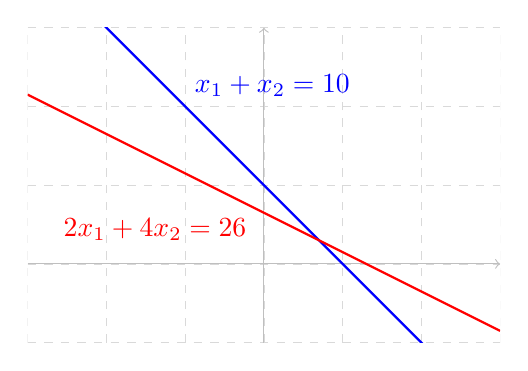
\begin{tikzpicture}[scale=0.1]
\pgfmathsetmacro{\A}{-30}
\pgfmathsetmacro{\B}{30}
\pgfmathsetmacro{\C}{-10}
\pgfmathsetmacro{\D}{30}
\coordinate (P) at (-10,20);
\coordinate (Q) at (-1,7);
\clip (\A,\C) rectangle (\B,\D);
\draw[help lines, color=gray!30, step=10, dashed] (\A,\C) grid (\B,\D);
\draw[->, color=gray!50] (\A,0)--(\B,0);
\draw[->, color=gray!50] (0,\C)--(0,\D);
\draw[thick, domain=\A:\B, samples=100, blue] plot ({\x}, {10-\x});
\draw[thick, domain=\A:\B, samples=100, red] plot ({\x}, {(13-\x)/2});
\node at (P)[above right] {\textcolor{blue}{$x_1+x_2=10$}};
\node at (Q)[below left] {\textcolor{red}{$2x_1+4x_2=26$}};
\end{tikzpicture}
\caption{Two lines intersect}
\label{fig: two lines intersect}
\end{subfigure}
\hfill
\begin{subfigure}[b]{0.4\textwidth}
\centering
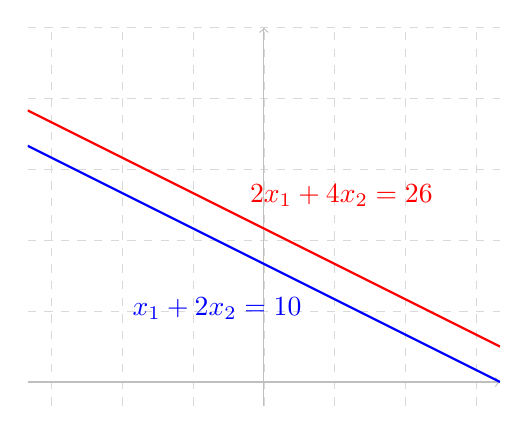
\begin{tikzpicture}[scale=0.3]
\pgfmathsetmacro{\A}{-10}
\pgfmathsetmacro{\B}{10}
\pgfmathsetmacro{\C}{-1}
\pgfmathsetmacro{\D}{15}
\coordinate (P) at (2,4);
\coordinate (Q) at (-1,7);
\clip (\A,\C) rectangle (\B,\D);
\draw[help lines, color=gray!30, step=3, dashed] (\A,\C) grid (\B,\D);
\draw[->, color=gray!50] (\A,0)--(\B,0);
\draw[->, color=gray!50] (0,\C)--(0,\D);
\draw[thick, domain=\A:\B, samples=100, blue] plot ({\x}, {(10-\x)/2});
\draw[thick, domain=\A:\B, samples=100, red] plot ({\x}, {(13-\x)/2});
\node at (P)[below left] {\textcolor{blue}{$x_1+2x_2=10$}};
\node at (Q)[above right] {\textcolor{red}{$2x_1+4x_2=26$}};
\end{tikzpicture}
\caption{Two lines parallel but not overlapping}
\label{fig: two lines parallel but not overlapping}
\end{subfigure}
\hfill
\vspace{3mm}
\begin{subfigure}[b]{0.4\textwidth}
\centering
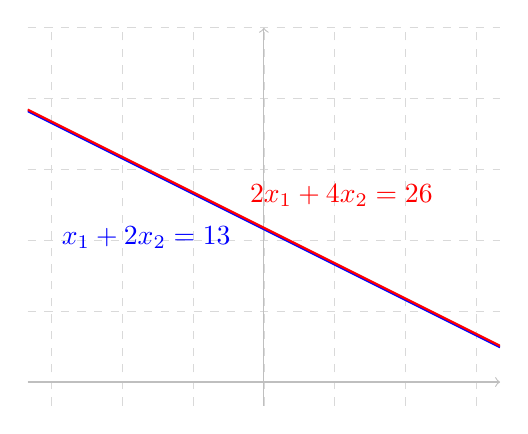
\begin{tikzpicture}[scale=0.3]
\pgfmathsetmacro{\A}{-10}
\pgfmathsetmacro{\B}{10}
\pgfmathsetmacro{\C}{-1}
\pgfmathsetmacro{\D}{15}
\pgfmathsetmacro{\E}{0.03}
\coordinate (Q) at (-1,7);
\clip (\A,\C) rectangle (\B,\D);
\draw[help lines, color=gray!30, step=3, dashed] (\A,\C) grid (\B,\D);
\draw[->, color=gray!50] (\A,0)--(\B,0);
\draw[->, color=gray!50] (0,\C)--(0,\D);
\draw[thick, domain=\A:\B, samples=100, blue] plot ({\x}, {(13-\x)/2-\E});
\draw[thick, domain=\A:\B, samples=100, red] plot ({\x}, {(13-\x)/2+\E});
\node at (Q)[below left] {\textcolor{blue}{$x_1+2x_2=13$}};
\node at (Q)[above right] {\textcolor{red}{$2x_1+4x_2=26$}};
\end{tikzpicture}
\caption{Two lines overlap}
\label{fig: two lines overlap}
\end{subfigure}
\caption{Figure for Example~\ref{ex: number of solutions}}
\label{fig: geometric interpretation of 2 by 2 linear system}
\end{figure}
\end{example}

If we increase the number of equations, we get more lines, it might looks like
\begin{figure}[H]
\centering
\begin{subfigure}[b]{0.2\textwidth}
\centering

\begin{tikzpicture}
\draw[help lines, color=gray!30, step=.4, dashed] (-1,-1) grid (1,1);
\draw(-1,0)--(1,0);
\draw(0,-1)--(0,1);
\draw(-1,-1)--(1,1);
\end{tikzpicture}
\end{subfigure}
\begin{subfigure}[b]{0.2\textwidth}
\centering
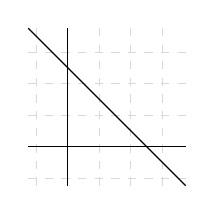
\begin{tikzpicture}[scale=0.5]
\draw[help lines, color=gray!30, step=.8, dashed] (-1,-1) grid (3,3);
\draw(-1,0)--(3,0);
\draw(0,-1)--(0,3);
\draw(-1,3)--(3,-1);
\end{tikzpicture}
\end{subfigure}
\begin{subfigure}[b]{0.2\textwidth}
\centering

\begin{tikzpicture}
\draw[help lines, color=gray!30, step=.4, dashed] (-1,-1) grid (1,1);
\draw(-1,0.5)--(1,0.5);
\draw(-1,-0.5)--(1,-0.5);
\draw(0,-1)--(0,1);
\end{tikzpicture}
\end{subfigure}
\begin{subfigure}[b]{0.2\textwidth}
\centering

\begin{tikzpicture}
\draw[help lines, color=gray!30, step=.4, dashed] (-1,-1) grid (1,1);
\draw(-1,0.5)--(1,0.5);
\draw(-1,-0.5)--(1,-0.5);
\draw(-1,0)--(1,0);
\end{tikzpicture}
\end{subfigure}
\end{figure}

If we increase the number of variables, we get
\begin{itemize}
\item $a_1x_1+a_2x_2+a_3x_3=b$ describes a plane in $\mathbb R^3$.
\item $a_1x_1+a_2x_2+a_3x_3+\cdots+a_nx_n=b$ describes a \textit{hyperplane} in $\mathbb R^n$.
\item Therefore the solution set of~\eqref{eq: general linear system} is the intersection of $m$ hyperplanes.
\end{itemize}

\begin{example}
Geometric interpretation of \systeme{x_1-3x_2+2x_3=0, -5x_1+12x_2-x_3=0}
\begin{center}
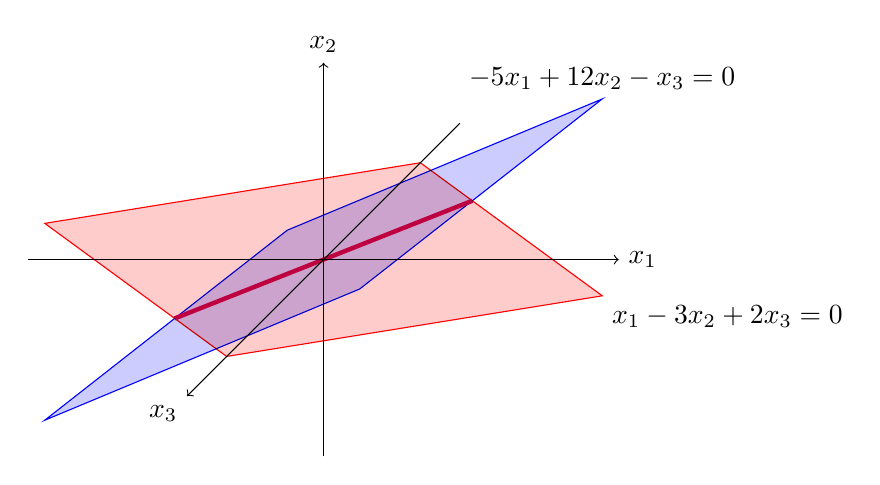
\begin{tikzpicture}
\definecolor{color1}{rgb}{255,0,0}
\definecolor{color2}{rgb}{0,0,255}
\definecolor{color3}{rgb}{255,0,255}
\def\XMAX{2.5};\def\YMAX{2.5};\def\ZMAX{4.5};
\begin{scope}[blend mode=multiply]
\draw [color1, fill=color1!20] plot (-2,-2,-2)--(-2,2,4)--(2,2,2)--(2,-2,-4)--cycle;
\node at (2,-2,-4) [below right]{$x_1-3x_2+2x_3=0$};
\draw [color2, fill=color2!20] plot (-2,-7/6,-4)--(-2,-1/2,4)--(2,7/6,4)--(2,1/2,-4)--cycle;
\node at (2,1/2,-4) [above]{$-5x_1+12x_2-x_3=0$};
\end{scope}
\draw [purple, ultra thick](-2,-6/7,-2/7)--(2,6/7,2/7);
\draw[->] (-1.5*\XMAX,0,0)--(1.5*\XMAX,0,0) node[right]{$x_1$};
\draw[->] (0,-\YMAX,0)--(0,\YMAX,0) node[above]{$x_2$};
\draw[->] (0,0,-\ZMAX)--(0,0,\ZMAX) node[below left]{$x_3$};
\end{tikzpicture}
\end{center}
\end{example}

\begin{remark}
It is geometrically clear that for a system of 2 equations in 3 variables, there are either no solutions or infinitely many, since two planes either intersects at a line, or overlap, or simply parallel.
\end{remark}

\begin{definition}
We say a linear system is \textcolor{blue}{consistent}\index{consistent} if it has solution(s), and \textcolor{blue}{inconsistent}\index{inconsistent} if it has none.
\end{definition}

\begin{example}
In the previous Example~\ref{ex: number of solutions}, \eqref{eq: unique solution} and~\eqref{eq: inf solutions} are consistent, while \eqref{eq: no solutions} is inconsistent
\end{example}

\begin{exercise}\hfill
\begin{enumerate}
\item Try Gaussian elimination on the following linear systems
\begin{enumerate}
\item \systeme{x_1+5x_2 = 7,-2x_1 - 7x_2 = -5 }
\item \systeme{2x_1+4x_2=-4, 5x_1+7x_2=11}
\item \systeme{x_1-x_2+x_3=1, 2x_1-x_3=1,x_1+x_2+x_3=3}
\end{enumerate}
\item Find the point of intersection of the lines $x_1-5x_2=1$ and $3x_1-7x_2=5$.
\item For what values of $h$ and $k$ is the following system consistent?
\[
\systeme{2x_1-x_2=h, -6x_1+3x_2=k}
\]
\end{enumerate}
\end{exercise}

\section{Lecture 2 - Matrices and row echelon form}

\subsection{Matrices}

\begin{definition}
A $m$ by $n$ (or $m\times n$) \textcolor{blue}{matrix}\index{matrix} is a rectangular array of numbers with $m$ rows and $n$ columns
\begin{equation}\label{eq: general m by n matrix}
\begin{bmatrix}
a_{11}&a_{12}&\cdots&a_{1n}\\
a_{21}&a_{22}&\cdots&a_{2n}\\
\vdots&\vdots&&\vdots\\
a_{m1}&a_{m2}&\cdots&a_{mn}
\end{bmatrix}
\end{equation}
We use the \textcolor{blue}{$(i,j)$-th entry} to mean the entry on the $i$-th row and $j$-column (i.e. $a_{ij}$).
\end{definition}

\begin{definition}
A matrix is
\begin{itemize}
\item a \textcolor{blue}{zero matrix}\index{zero matrix} is a matrix with all entries zeros.
\[
\begin{bmatrix}
0&0&\cdots&0\\
0&0&\cdots&0\\
\vdots&\vdots&&\vdots\\
0&0&\cdots&0
\end{bmatrix}
\]
\item a \textcolor{blue}{square matrix}\index{square matrix} is a matrix with the same number of rows and columns, i.e. $m=n$.
\[
\begin{bmatrix}
a_{11}&a_{12}&\cdots&a_{1n}\\
a_{21}&a_{22}&\cdots&a_{2n}\\
\vdots&\vdots&&\vdots\\
a_{n1}&a_{n2}&\cdots&a_{nn}
\end{bmatrix}
\]
\item a \textcolor{blue}{vector}\index{vector} if it only has one column, i.e. $n=1$.
\[
\begin{bmatrix}
a_{1}\\a_{2}\\\vdots\\a_{m}
\end{bmatrix}
\]
\item a \textcolor{blue}{row vector}\index{row vector} if it only has one row, i.e. $m=1$.
\[
\begin{bmatrix}
a_{1}&a_{2}&\cdots&a_{n}
\end{bmatrix}
\]
\item the \textcolor{blue}{identity matrix}\index{identity matrix} if it is a square matrix with diagonal elements 1's, and 0's otherwise. Here the diagonal are the $(i,i)$-th entries.
\[
\begin{bmatrix}
1&0&\cdots&0\\
0&1&\cdots&0\\
\vdots&\vdots&\ddots&\vdots\\
0&0&\cdots&1
\end{bmatrix}
\]
\end{itemize}
\end{definition}

\begin{definition}
Soon we will be getting tired of writing all these equations in the linear system~\eqref{eq: general linear system}, instead we write down its \textcolor{blue}{augmented matrix}\index{augmented matrix}
\[
\begin{bmatrix}
a_{11}&a_{12}&a_{13}&\cdots&a_{1n}&b_1\\
a_{21}&a_{22}&a_{23}&\cdots&a_{2n}&b_2\\
a_{31}&a_{32}&a_{33}&\cdots&a_{1n}&b_3\\
\vdots&\vdots&\vdots&&\vdots\\
a_{m1}&a_{m2}&a_{m3}&\cdots&a_{mn}&b_m
\end{bmatrix}
\]
Which is obtained by omitting $x_i$'s, pluses, and equal signs. If we delete the last column, we will get the \textcolor{blue}{coefficient matrix}\index{coefficient matrix}
\[
\begin{bmatrix}
a_{11}&a_{12}&a_{13}&\cdots&a_{1n}\\
a_{21}&a_{22}&a_{23}&\cdots&a_{2n}\\
a_{31}&a_{32}&a_{33}&\cdots&a_{1n}\\
\vdots&\vdots&\vdots&&\vdots\\
a_{m1}&a_{m2}&a_{m3}&\cdots&a_{mn}
\end{bmatrix}
\]
\end{definition}

\begin{example}\hfill
\begin{itemize}
\item For \eqref{14:34-05/31/2022}, its augmented matrix and coefficient matrix are
\[
\begin{bmatrix}
1&1&10\\
2&4&26
\end{bmatrix},\begin{bmatrix}
1&1\\
2&4
\end{bmatrix}
\]
\item For \systeme{x_1-x_2+x_3=1, 2x_1-x_3=1,x_1+x_2+x_3=3}, its augmented matrix and coefficient matrix are
\[
\begin{bmatrix}
1&-1&1&1\\
2&0&-1&1\\
1&1&1&3
\end{bmatrix},\begin{bmatrix}
1&-1&1\\
2&0&-1\\
1&1&1
\end{bmatrix}
\]
\item In general, a linear system of $m$ equations in $n$ variables has a $m$ by $(n+1)$ augmented matrix and a $m$ by $n$ coefficient matrix.
\end{itemize}
\end{example}

\begin{definition}
Inspired by Gaussian elimination, we define the following three \textcolor{blue}{elementary row operations}\index{elementary row operations}
\begin{itemize}
\item \textcolor{blue}{Replacement}\index{row replacement}: Replace one row by the sum of itself and a multiple of another row.
\item \textcolor{blue}{Interchangement}\index{row interchange}: Interchange two rows.
\item \textcolor{blue}{Scaling}\index{row scaling}: Multiply all entries in a row by a \textit{nonzero} constant.
\end{itemize}
We say matrices $A,B$ are \textcolor{blue}{row equivalent}\index{row equivalence} ($A\sim B$) if $B$ can obtained by applying a sequence of elementary row operations to $A$ (or vise versa).
\end{definition}

\begin{example}
Let's rewrite the process in Example~\ref{13:09-05/31/2022}
\begin{align*}
&\begin{bmatrix}
1&1&10\\
2&4&26
\end{bmatrix}\xsim{R2\rightarrow R2-2R1}
\begin{bmatrix}
1&1&10\\
0&2&6
\end{bmatrix}\xsim{R2\rightarrow\frac{R2}{2}}
\begin{bmatrix}
1&1&10\\
0&1&3
\end{bmatrix}\xsim{R1\rightarrow R1-R2}
\begin{bmatrix}
1&0&7\\
0&1&3
\end{bmatrix}
\end{align*}
\end{example}

\begin{example}\label{18:10-06/01/2022}
Solve \systeme{x_1-x_2+x_3=1, 2x_1-x_3=1,x_1+x_2+x_3=3} with augmented matrix.
\begin{align*}
&\begin{bmatrix}
1&-1&1&1\\
2&0&-1&1\\
1&1&1&3\\
\end{bmatrix}\xsim{R2\rightarrow R2-2R1}\begin{bmatrix}
1&-1&1&1\\
0&2&-3&-1\\
1&1&1&3\\
\end{bmatrix}\xsim{R3\rightarrow R3-R1}\begin{bmatrix}
1&-1&1&1\\
0&2&-3&-1\\
0&2&0&2\\
\end{bmatrix}\\
&\xsim{R3\rightarrow R3-R2}\begin{bmatrix}
1&-1&1&1\\
0&2&-3&-1\\
0&0&3&3\\
\end{bmatrix}\xsim{R3\to\frac{R3}{3}}\begin{bmatrix}
1&-1&1&1\\
0&2&-3&-1\\
0&0&1&1\\
\end{bmatrix}\xsim{\substack{R1\rightarrow R1-R3\\R2\rightarrow R2+3R3}}\begin{bmatrix}
1&-1&0&0\\
0&2&0&2\\
0&0&1&1\\
\end{bmatrix}\\
&\xsim{R2\to\frac{R2}{2}}\begin{bmatrix}
1&-1&0&0\\
0&1&0&1\\
0&0&1&1\\
\end{bmatrix}\xsim{R1\rightarrow R1+R2}\begin{bmatrix}
1&0&0&1\\
0&1&0&1\\
0&0&1&1\\
\end{bmatrix}
\end{align*}
This gives the unique solution \systeme*{x_1=1, x_2=1, x_3=1}
\end{example}

\subsection{Row echelon form}

\begin{definition}\hfill
\begin{itemize}
\item A \textcolor{blue}{leading entry}\index{leading entry} of a row refers to the leftmost nonzero entry (in a nonzero row).
\item A matrix is of \textcolor{blue}{row echelon form (REF)}\index{row echelon form (REF)} if it is of a ``staircase shape".
\[
\overset{\text{REF}}{
\begin{bmatrix}
\blacksquare&*&*&*&*&*&*&*\\
0&0&\blacksquare&*&*&*&*&*\\
0&0&0&0&\blacksquare&*&*&*\\
0&0&0&0&0&\blacksquare&*&*\\
\end{bmatrix}
}
\]
$\blacksquare$ are the leading entries, $*$ are some unknown numbers.
\item The leading entries of an REF matrix are called \textcolor{blue}{pivots}\index{pivot}.
\item The position of pivots are called \textcolor{blue}{pivot positions}\index{pivot positions}.
\item The column pivots are in are called \textcolor{blue}{pivot columns}\index{pivot columns}.
\item An REF of \textcolor{blue}{reduced row echelon form (RREF)}\index{reduced row echelon form, RREF} if all its pivots are 1's and in each pivot column, every entry except the pivot are 0's.
\end{itemize}
\[
\overset{\text{RREF}}{\begin{bmatrix}
1&*&0&*&0&0&*&*\\
0&0&1&*&0&0&*&*\\
0&0&0&0&1&0&*&*\\
0&0&0&0&0&1&*&*\\
\end{bmatrix}
}
\]
\end{definition}

\begin{example}
In Example~\ref{18:10-06/01/2022}, $\begin{bmatrix}
1&-1&1&1\\
0&2&-3&-1\\
0&2&0&2\\
\end{bmatrix}$ is not an REF. $\begin{bmatrix}
1&-1&1&1\\
0&2&-3&-1\\
0&0&3&3\\
\end{bmatrix}$ is an REF, but not an RREF. $\begin{bmatrix}
1&0&0&1\\
0&1&0&1\\
0&0&1&1\\
\end{bmatrix}$ is an RREF
\end{example}

\begin{theorem}\label{18:46-06/08/2022}
Every matrix is row equivalent to some REF matrix (which is not in general unique), but it is row equivalent to some unique RREF matrix.
\end{theorem}

% \begin{remark}
% This ensures that the pivot positions are well-defined, i.e. you won't get different pivot positions if you applied different row operations
% \end{remark}

\begin{example}
In Example~\ref{18:10-06/01/2022}, $\begin{bmatrix}
1&-1&1&1\\
0&2&-3&-1\\
0&0&3&3\\
\end{bmatrix}$ is an REF that is row equivalent to the original matrix $\begin{bmatrix}
1&-1&1&1\\
2&0&-1&1\\
1&1&1&3\\
\end{bmatrix}$, and $\begin{bmatrix}
1&0&0&1\\
0&1&0&1\\
0&0&1&1\\
\end{bmatrix}$ is its unique row equivalent RREF.
\end{example}

% \begin{remark}
% A linear system has a unique solution if and only if its RREF deleting the last column gives the identity matrix.
% \end{remark}

\begin{example}\label{ex: no solution system}
Solve \systeme{x_1-x_2+x_3=1, 2x_1-x_3=1,x_1+x_2-2x_3=1} with augmented matrix.
\begin{align*}
&\begin{bmatrix}
1&-1&1&1\\
2&0&-1&1\\
1&1&-2&1\\
\end{bmatrix}\xsim{\substack{R2\rightarrow R2-2R1\\R3\rightarrow R3-R1}}\begin{bmatrix}
1&-1&1&1\\
0&2&-3&-1\\
0&2&-3&0\\
\end{bmatrix}\xsim{R3\rightarrow R3-R2}\begin{bmatrix}
1&-1&1&1\\
0&2&-3&-1\\
0&0&0&1\\
\end{bmatrix}
\end{align*}
You might notice that the last row represents $0x_1+0x_2+0x_3=1$, this is a contradiction, therefore the linear system is inconsistent.
\end{example}

% \begin{remark}
% This only happens if and only if the last pivot column is the last column
% \end{remark}

\begin{example}\label{09:47-06/02/2022}
\systeme{x_1-x_2+x_3=1, 2x_1-x_3=1}, we write down its augmented matrix
\begin{align*}
&\begin{bmatrix}
1&-1&1&1\\
2&0&-1&1\\
\end{bmatrix}\xsim{R2\rightarrow R2-2R1}\begin{bmatrix}
1&-1&1&1\\
0&2&-3&-1\\
\end{bmatrix}\\
&\xsim{\frac{R2}{2}}\begin{bmatrix}
1&-1&1&1\\
0&1&-\frac{3}{2}&-\frac{1}{2}\\
\end{bmatrix}\xsim{R1\rightarrow R1+R2}\begin{bmatrix}
1&0&-\frac{1}{2}&\frac{1}{2}\\
0&1&-\frac{3}{2}&-\frac{1}{2}\\
\end{bmatrix}
\end{align*}
This gives the solution set
\begin{equation}
\systeme{x_1-\frac{1}{2}x_3=\frac{1}{2}, x_2-\frac{3}{2}x_3=\frac{1}{2}}\Rightarrow\systeme*{x_1=\frac{1}{2}x_3+\frac{1}{2}, x_2=\frac{3}{2}x_3-\frac{1}{2}}
\end{equation}
\end{example}

Let's formalize these as \textcolor{blue}{row reduction algorithm}\index{row reduction algorithm}
\begin{enumerate}[label=Step \arabic*.]
\item Begin with the leftmost nonzero column. This is a pivot column. The pivot position should be at the top. 
\item Select a nonzero entry in the pivot column as a pivot. If necessary, interchange rows to move this entry into the pivot position.
\item Use row replacement operations to create zeros in all positions below the pivot. 
\item Cover (or ignore) the rows containing the pivot positions. Apply Steps 1-3 to the rows that remains. Repeat the process until you are left with an REF.
\item Beginning with the rightmost pivot and working upward and to the left, create zeros above each pivot. If a pivot is not 1, make it 1 by a scaling operation. 
\end{enumerate}
Steps 1-4 are call \textcolor{blue}{forward phase}, after which you get an REF. Step 5 is called \textcolor{blue}{backward phase}, after which you get the RREF.

\begin{example}
Consider the augmented matrix $\begin{bmatrix}
0&-3&-6&4&9\\
-1&-2&-1&3&1\\
-2&-3&0&3&-1\\
1&4&5&-9&-7\\
\end{bmatrix}$
\begin{itemize}[leftmargin=*]
\item Forward phase
\[
\begin{bmatrix}
0&-3&-6&4&9\\
-1&-2&-1&3&1\\
-2&-3&0&3&-1\\
1&4&5&-9&-7\\
\end{bmatrix}\xsim{\substack{R1\leftrightarrow R4\\\text{Step 1,2}}}\begin{bmatrix}
1&4&5&-9&-7\\
-1&-2&-1&3&1\\
-2&-3&0&3&-1\\
0&-3&-6&4&9\\
\end{bmatrix}
\]
\[
\begin{bmatrix}
1&4&5&-9&-7\\
-1&-2&-1&3&1\\
-2&-3&0&3&-1\\
0&-3&-6&4&9\\
\end{bmatrix}\xsim{\substack{R2\rightarrow R2+R1\\R3\rightarrow R3+2R1\\\text{Step 3}}}\begin{bmatrix}
1&4&5&-9&-7\\
0&2&4&-6&-6\\
0&5&10&-15&-15\\
0&-3&-6&4&9\\
\end{bmatrix}
\]
\[
\begin{bmatrix}
1&4&5&-9&-7\\
0&2&4&-6&-6\\
0&5&10&-15&-15\\
0&-3&-6&4&9\\
\end{bmatrix}\xsim{\substack{R3\rightarrow R3-\frac{5}{2}R2\\R4\rightarrow R4+\frac{3}{2}R2\\\text{Step 4,1,2,3}}}\begin{bmatrix}
1&4&5&-9&-7\\
0&2&4&-6&-6\\
0&0&0&0&0\\
0&0&0&-5&0\\
\end{bmatrix}
\]
\[
\begin{bmatrix}
1&4&5&-9&-7\\
0&2&4&-6&-6\\
0&0&0&0&0\\
0&0&0&-5&0\\
\end{bmatrix}\xsim{\substack{R3\leftrightarrow R4\\\text{Step 4,1}}}\begin{bmatrix}
1&4&5&-9&-7\\
0&2&4&-6&-6\\
0&0&0&-5&0\\
0&0&0&0&0\\
\end{bmatrix}
\]
\item Backward phase
\begin{align*}
&\begin{bmatrix}
1&4&5&-9&-7\\
0&2&4&-6&-6\\
0&0&0&-5&0\\
0&0&0&0&0\\
\end{bmatrix}\xsim{\substack{R3\rightarrow R3/(-5)\\\text{Step 5}}}\begin{bmatrix}
1&4&5&-9&-7\\
0&2&4&-6&-6\\
0&0&0&1&0\\
0&0&0&0&0\\
\end{bmatrix}\xsim{\substack{R1\rightarrow R1+9R3\\R2\rightarrow R2+6R3\\\text{Step 5}}}\begin{bmatrix}
1&4&5&0&-7\\
0&2&4&0&-6\\
0&0&0&1&0\\
0&0&0&0&0\\
\end{bmatrix}\\
&\xsim{\substack{R2\rightarrow R2/2\\\text{Step 5}}}\begin{bmatrix}
1&4&5&0&-7\\
0&1&2&0&-3\\
0&0&0&1&0\\
0&0&0&0&0\\
\end{bmatrix}\xsim{\substack{R1\rightarrow R1-4R2\\\text{Step 5}}}\begin{bmatrix}
1&0&-3&0&5\\
0&1&2&0&-3\\
0&0&0&1&0\\
0&0&0&0&0\\
\end{bmatrix}
\end{align*}
\end{itemize}
\end{example}

\begin{definition}
The variables corresponding to pivot columns in a matrix are called \textcolor{blue}{basic variables}\index{basic variable}, the other variables are called \textcolor{blue}{free variables}\index{free variable}. In a solution set, basic variables are expressed in terms of free variables, and a free variable can take any value.
\end{definition}

\begin{example}
In Example~\ref{09:47-06/02/2022}, $x_1,x_2$ are basic variables and $x_3$ is a free variable. And we formally write our solution set as $\begin{cases}
x_1=\frac{1}{2}x_3+\frac{1}{2} \\
x_2=\frac{3}{2}x_3-\frac{1}{2} \\
x_3\text{ is free}
\end{cases}$
\end{example}

\begin{exercise}\label{08:47-06/06/2022}
Find the general solution of the system \systeme{x_1-2x_2-x_3 + 3x_4 = 0, -2x_1 + 4x_2 + 5x_3 - 5x_4 = 3, 3x_1 - 6x_2 - 4x_3 + 8x_4 = 2}
\end{exercise}

\begin{solution}
\begin{align*}
&\begin{bmatrix}
1&-2&-1&3&0\\
-2&4&5&-5&3\\
3&-6&-4&8&2\\
\end{bmatrix}\xsim{\substack{R2\rightarrow R2+2R1\\R3\rightarrow R3-3R1}}\begin{bmatrix}
1&-2&-1&3&0\\
0&0&3&1&3\\
0&0&-1&-1&2\\
\end{bmatrix}\xsim{R3\to(-1)\cdot R3}\begin{bmatrix}
1&-2&-1&3&0\\
0&0&3&1&3\\
0&0&1&1&-2\\
\end{bmatrix}\\
&\xsim{R2\rightarrow R2-3R3}\begin{bmatrix}
1&-2&-1&3&0\\
0&0&0&-2&9\\
0&0&1&1&-2\\
\end{bmatrix}\xsim{R2\leftrightarrow R3}\begin{bmatrix}
1&-2&-1&3&0\\
0&0&1&1&-2\\
0&0&0&-2&9\\
\end{bmatrix}\\
&\xsim{R3\to\frac{R3}{-2}}\begin{bmatrix}
1&-2&-1&3&0\\
0&0&1&1&-2\\
0&0&0&1&-\frac{9}{2}\\
\end{bmatrix}\xsim{\substack{R2\rightarrow R2-R3\\R1\rightarrow R1-3R3}}\begin{bmatrix}
1&-2&-1&0&\frac{27}{2}\\
0&0&1&0&\frac{5}{2}\\
0&0&0&1&-\frac{9}{2}\\
\end{bmatrix}\xsim{R1\rightarrow R1+R2}\begin{bmatrix}
1&-2&0&0&16\\
0&0&1&0&\frac{5}{2}\\
0&0&0&1&-\frac{9}{2}\\
\end{bmatrix}
\end{align*}
Write this as solution set, we get
\[
\systeme*{x_1-2x_2=16, x_3=\frac{5}{2}, x_4=-\frac{9}{2}}\Rightarrow
\begin{cases}
x_1=2x_2+16\\
x_2\text{ is free}\\
x_3=\frac{5}{2}\\
x_4=-\frac{9}{2}
\end{cases}
\]
\end{solution}

\begin{theorem}\label{14:16-06/03/2022}
Suppose the augmented matrix of a linear system is $\begin{bmatrix}
A&\mathbf b
\end{bmatrix}$, and its RREF is $\begin{bmatrix}
U&\mathbf d
\end{bmatrix}$, then the linear system has
\begin{itemize}
\item no solutions $\iff \mathbf d$ is a pivot column, i.e. contains a pivot.
\item has solutions $\iff\mathbf d$ is not a pivot column
\begin{itemize}
\item a unique solution $\iff$ every column of $U$ is a pivot column.
\item infinitely many solutions $\iff$ some columns of $U$ is not a pivot column.
\end{itemize}
\end{itemize}
\end{theorem}

\begin{example}\hfill
\begin{itemize}
\item In Example~\ref{ex: no solution system}, the linear system has no solutions since
\[
\begin{bmatrix}
A&\mathbf b
\end{bmatrix}=
\begin{bmatrix}
1&-1&1&1\\
2&0&-1&1\\
1&1&-2&1\\
\end{bmatrix}\sim\begin{bmatrix}
1&-1&1&1\\
0&2&-3&-1\\
0&0&0&1\\
\end{bmatrix}=\begin{bmatrix}
U&\mathbf d
\end{bmatrix}
\]
\item In Example~\ref{18:10-06/01/2022}, the linear system has a unique solution since
\[
\begin{bmatrix}
A&\mathbf b
\end{bmatrix}=\begin{bmatrix}
1&−1 &1& 1\\
2&0 &−1 &1\\
1&1&1 &3
\end{bmatrix}\sim\begin{bmatrix}
1&0&0&1\\
0&1&0&1\\
0&0&1&1\\
\end{bmatrix}=\begin{bmatrix}
U&\mathbf d
\end{bmatrix}
\]
\item In Example~\ref{08:47-06/06/2022}, the linear system has infinitely many solutions since
\[
\begin{bmatrix}
A&\mathbf b
\end{bmatrix}=\begin{bmatrix}
1&-2&-1&3&0\\
-2&4&5&-5&3\\
3&-6&-4&8&2\\
\end{bmatrix}\sim\begin{bmatrix}
1&-2&0&0&16\\
0&0&1&0&\frac{5}{2}\\
0&0&0&1&-\frac{9}{2}\\
\end{bmatrix}=\begin{bmatrix}
U&\mathbf d
\end{bmatrix}
\]
\end{itemize}
\end{example}

\begin{exercise}
Find the general solutions of the system with given augmented matrix, name the pivot columns, pivot positions, basic and free variables.
\begin{enumerate}
\item $\begin{bmatrix}
0&1&-6&5\\
1&-2&7&-4\\
\end{bmatrix}$
\item $\begin{bmatrix}
1&-7&0&6&5\\
0&0&1&-2&-3\\
-1&7&-4&2&7
\end{bmatrix}$
\end{enumerate}
\end{exercise}

\begin{question}
How does the size of the augmented matrix affect the solution set?
\end{question}

\section{Lecture 3 - Matrix algebra}

\subsection{Matrix addition and scalar multiplication}

\begin{definition}
Let's use $M_{m\times n}(\mathbb R)$ to denote the set of all (real-valued) $m$ by $n$ matrices.
\end{definition}

\begin{definition}
Suppose $A,B$ are $m\times n$ matrices, $c$ is a scalar (i.e. a number), then we can define
\begin{itemize}
\item Addition
\begin{align*}
&\begin{bmatrix}
a_{11}&a_{12}&\cdots&a_{1n}\\
a_{21}&a_{22}&\cdots&a_{2n}\\
\vdots&\vdots&&\vdots\\
a_{m1}&a_{m2}&\cdots&a_{mn}
\end{bmatrix}+\begin{bmatrix}
b_{11}&b_{12}&\cdots&b_{1n}\\
b_{21}&b_{22}&\cdots&b_{2n}\\
\vdots&\vdots&&\vdots\\
b_{m1}&b_{m2}&\cdots&b_{mn}
\end{bmatrix}\\
&=\begin{bmatrix}
a_{11}+b_{11}&a_{12}+b_{12}&\cdots&a_{1n}+b_{1n}\\
a_{21}+b_{21}&a_{22}+b_{22}&\cdots&a_{2n}+b_{2n}\\
\vdots&\vdots&&\vdots\\
a_{m1}+b_{m1}&a_{m2}+b_{m2}&\cdots&a_{mn}+b_{mn}
\end{bmatrix}
\end{align*}
\item Scalar multiplication
\[
c\begin{bmatrix}
a_{11}&a_{12}&\cdots&a_{1n}\\
a_{21}&a_{22}&\cdots&a_{2n}\\
\vdots&\vdots&&\vdots\\
a_{m1}&a_{m2}&\cdots&a_{mn}
\end{bmatrix}=\begin{bmatrix}
ca_{11}&ca_{12}&\cdots&ca_{1n}\\
ca_{21}&ca_{22}&\cdots&ca_{2n}\\
\vdots&\vdots&&\vdots\\
ca_{m1}&ca_{m2}&\cdots&ca_{mn}
\end{bmatrix}
\]
\end{itemize}
\end{definition}

\begin{example}\hfill
\begin{itemize}
\item $\begin{bmatrix}
1&2\\
3&4
\end{bmatrix}+\begin{bmatrix}
4&3\\
2&1
\end{bmatrix}=\begin{bmatrix}
5&5\\
5&5
\end{bmatrix}$
\item $2\begin{bmatrix}
1&2\\
3&4
\end{bmatrix}=\begin{bmatrix}
2&4\\
6&8
\end{bmatrix}$
\end{itemize}
\end{example}

\subsection{Matrix multiplication}

\begin{definition}
Suppose $A$ is a $m\times n$ matrix, and $B$ is a $n\times p$ matrix, we can define \textcolor{blue}{matrix multiplication}\index{matrix multiplication} $AB$ to be the $m\times p$ matrix, computed via the \textcolor{blue}{row-column rule}\index{rule-column rule}: The $(i,j)$-entry is to multiply the $i$-row and $j$-th column
\[
\begin{bmatrix}
\\
\\
\\
a_{i1}&a_{i2}&\cdots &a_{in}\\
\\
\\
\end{bmatrix}\begin{bmatrix}
&&b_{1j}&&&\\
&&b_{2j}&&&\\
&&\vdots&&&\\
&&b_{nj}&&&\\
\end{bmatrix}=\begin{bmatrix}
&&&&&\\
&&&&&\\
&&&&&\\
&&\blacksquare&&\\
&&&&&\\
&&&&&
\end{bmatrix}
\]
Where the $(i,j)$-entry $\blacksquare=a_{i1}b_{1j}+a_{i2}b_{2j}+\cdots+a_{in}b_{nj}$.

If $A$ is a square matrix, then we could define matrix power $A^k$ to be simply $\overbrace{AA\cdots A}^{k\text{ times}}$
\end{definition}

\begin{example}\hfill
\begin{itemize}
\item $\begin{bmatrix}
a_{11}&a_{12}&a_{13}\\
a_{21}&a_{22}&a_{23}
\end{bmatrix}
\begin{bmatrix}
b_{11}&b_{12}\\
b_{21}&b_{22}\\
b_{31}&b_{32}
\end{bmatrix}=\begin{bmatrix}
a_{11}b_{11}+a_{12}b_{21}+a_{13}b_{31} & a_{11}b_{12}+a_{12}b_{22}+a_{13}b_{32}\\
a_{21}b_{11}+a_{22}b_{21}+a_{23}b_{31} & a_{21}b_{12}+a_{22}b_{22}+a_{23}b_{32}
\end{bmatrix}$
\item $\begin{bmatrix}
1&2&2\\
2&1&1
\end{bmatrix}\begin{bmatrix}
3&1\\
1&2\\
2&3
\end{bmatrix}=\begin{bmatrix}
1\cdot3+2\cdot1+2\cdot2&1\cdot1+2\cdot2+2\cdot3\\
2\cdot3+1\cdot1+1\cdot2&2\cdot1+1\cdot2+1\cdot3
\end{bmatrix}=\begin{bmatrix}
9&11\\
9&7
\end{bmatrix}$
\item
\begin{equation}\label{15:02-06/03/2022}
\begin{bmatrix}
a_{11}&a_{12}&a_{13}\\
a_{21}&a_{22}&a_{23}
\end{bmatrix}
\begin{bmatrix}
x_1\\
x_2\\
x_3
\end{bmatrix}=\begin{bmatrix}
a_{11}x_1+a_{12}x_2+a_{13}x_3 \\
a_{21}x_1+a_{22}x_2+a_{23}x_3
\end{bmatrix}=x_1\begin{bmatrix}a_{11}\\a_{21}\end{bmatrix}+x_1\begin{bmatrix}a_{12}\\a_{22}\end{bmatrix}+x_1\begin{bmatrix}a_{13}\\a_{23}\end{bmatrix}
\end{equation}
\item
\begin{equation}\label{15:13-06/03/2022}
\begin{bmatrix}
0&1\\
0&0
\end{bmatrix}\begin{bmatrix}
1&0\\
0&0
\end{bmatrix}=\begin{bmatrix}
0\cdot1+1\cdot0&0\cdot0+1\cdot0\\
0\cdot1+0\cdot0&0\cdot0+0\cdot0
\end{bmatrix}=\begin{bmatrix}
0&0\\
0&0
\end{bmatrix}
\end{equation}
\item
\begin{equation}\label{AB not BA}
\begin{bmatrix}
1&0\\
0&0
\end{bmatrix}\begin{bmatrix}
0&1\\
0&0
\end{bmatrix}=\begin{bmatrix}
1\cdot0+0\cdot0&1\cdot1+0\cdot0\\
0\cdot0+0\cdot0&0\cdot1+0\cdot0
\end{bmatrix}=\begin{bmatrix}
0&1\\
0&0
\end{bmatrix}
\end{equation}
\item 
\[
\begin{bmatrix}
a_{11}&a_{12}&a_{13}\\
a_{21}&a_{22}&a_{23}\\
a_{31}&a_{32}&a_{33}\\
\end{bmatrix}\begin{bmatrix}
1&0&0\\
0&1&0\\
0&0&1
\end{bmatrix}=\begin{bmatrix}
a_{11}&a_{12}&a_{13}\\
a_{21}&a_{22}&a_{23}\\
a_{31}&a_{32}&a_{33}\\
\end{bmatrix}
\]
\item 
\[
\begin{bmatrix}
1&0&0\\
0&1&0\\
0&0&1
\end{bmatrix}\begin{bmatrix}
a_{11}&a_{12}&a_{13}\\
a_{21}&a_{22}&a_{23}\\
a_{31}&a_{32}&a_{33}\\
\end{bmatrix}=\begin{bmatrix}
a_{11}&a_{12}&a_{13}\\
a_{21}&a_{22}&a_{23}\\
a_{31}&a_{32}&a_{33}\\
\end{bmatrix}
\]
\end{itemize}
\end{example}

\begin{example}\label{ex: elementary matrices}\hfill
\begin{enumerate}
\item 
\[
\begin{bmatrix}
1&0&-3\\
0&1&0\\
0&0&1
\end{bmatrix}\begin{bmatrix}
a_{11}&a_{12}&a_{13}\\
a_{21}&a_{22}&a_{23}\\
a_{31}&a_{32}&a_{33}\\
\end{bmatrix}=\begin{bmatrix}
a_{11}-3a_{31}&a_{12}-3a_{32}&a_{13}-3a_{33}\\
a_{21}&a_{22}&a_{23}\\
a_{31}&a_{32}&a_{33}\\
\end{bmatrix}
\]
\item 
\[
\begin{bmatrix}
a_{11}&a_{12}&a_{13}\\
a_{21}&a_{22}&a_{23}\\
a_{31}&a_{32}&a_{33}
\end{bmatrix}\begin{bmatrix}
1&0&0\\
0&1&0\\
2&0&1
\end{bmatrix}=\begin{bmatrix}
a_{11}+2a_{13}&a_{12}&a_{13}\\
a_{21}+2a_{23}&a_{22}&a_{23}\\
a_{31}+2a_{33}&a_{32}&a_{33}\\
\end{bmatrix}
\]
\item 
\[
\begin{bmatrix}
1&0&0\\
0&2&0\\
0&0&1
\end{bmatrix}\begin{bmatrix}
a_{11}&a_{12}&a_{13}\\
a_{21}&a_{22}&a_{23}\\
a_{31}&a_{32}&a_{33}
\end{bmatrix}=\begin{bmatrix}
a_{11}&a_{12}&a_{13}\\
2a_{21}&2a_{22}&2a_{23}\\
a_{31}&a_{32}&a_{33}
\end{bmatrix}
\]
\item 
\[
\begin{bmatrix}
a_{11}&a_{12}&a_{13}\\
a_{21}&a_{22}&a_{23}\\
a_{31}&a_{32}&a_{33}
\end{bmatrix}\begin{bmatrix}
1&0&0\\
0&3&0\\
0&0&1
\end{bmatrix}=\begin{bmatrix}
a_{11}&3a_{12}&a_{13}\\
a_{21}&3a_{22}&a_{23}\\
a_{31}&3a_{32}&a_{33}
\end{bmatrix}
\]
\item 
\[
\begin{bmatrix}
0&0&1\\
0&1&0\\
1&0&0
\end{bmatrix}\begin{bmatrix}
a_{11}&a_{12}&a_{13}\\
a_{21}&a_{22}&a_{23}\\
a_{31}&a_{32}&a_{33}
\end{bmatrix}=\begin{bmatrix}
a_{31}&a_{32}&a_{33}\\
a_{21}&a_{22}&a_{23}\\
a_{11}&a_{12}&a_{13}
\end{bmatrix}
\]
\item 
\[
\begin{bmatrix}
a_{11}&a_{12}&a_{13}\\
a_{21}&a_{22}&a_{23}\\
a_{31}&a_{32}&a_{33}
\end{bmatrix}\begin{bmatrix}
0&1&0\\
1&0&0\\
0&0&1
\end{bmatrix}=\begin{bmatrix}
a_{12}&a_{11}&a_{13}\\
a_{22}&a_{21}&a_{23}\\
a_{32}&a_{31}&a_{33}
\end{bmatrix}
\]
\end{enumerate}
\end{example}

\begin{exercise}
Suppose $A=\begin{bmatrix}
1&1&1\\
2&2&1\\
2&1&1
\end{bmatrix}, B=\begin{bmatrix}
1&1&1\\
2&2&1\\
2&1&1
\end{bmatrix}$, computes matrix multiplication $AB$
\end{exercise}

\begin{fact}\label{19:08-06/07/2022}
Suppose $A,B,C,D$ are matrices, $c$ is a scalar, $0$ is the zero matrix, $I$ is the identity matrix. we have the following facts
\begin{enumerate}[label=\alph*)]
\item Matrix multiplication is generally \textit{NOT commutative}, i.e. $AB\neq BA$
\item Matrix multiplication is \textit{associative}, i.e. the order of multiplication doesn't matter, in other words $(AB)C=A(BC)$, so it makes sense to write successive multiplication $A_1A_2A_3\cdots A_n$
\item Scalar multiplication and matrix multiplication commutes, $A(cB)=c(AB)=(cA)B$. so it makes sense to write $cA_1A_2A_3\cdots A_n$
\item Matrix multiplication is \textit{distributive} over addition, i.e. $A(B+C)=AB+AC$, $(A+B)C=AC+BC$
\item Zero matrix and identity matrix acts as 0 and 1, i.e. $A+0=0+A=A$, $A0=0A=0$, $IA=AI=A$
\item Even if $A\neq0$, $B\neq0$, $AB$ could still be $0$, take \eqref{15:13-06/03/2022} for an example
\item $AB=AC$ does NOT imply $B=C$
\end{enumerate}
\end{fact}

\begin{remark}
Some of the properties of matrices are really similar to that of numbers, so we dub this the name of \textit{matrix algebra}
\end{remark}

\subsection{Partitioned matrix}

\begin{definition}
$A$ is a \textcolor{blue}{partitioned} (or \textcolor{blue}{block}) matrix\index{partitioned matrix} if is divided into smaller submatrix by some horizontal and vertical lines. And the submatrices are the blocks
\begin{center}
$\left[\begin{array}{c|c|c}
A_{11}&A_{12}&A_{13}\\
\hline
A_{21}&A_{22}&A_{23}\\
\hline
A_{31}&A_{32}&A_{33}\\
\end{array}\right]=
\left[\begin{array}{cc|cccc|c}
a_{11}&a_{12}&a_{13}&a_{14}&a_{15}&a_{16}&a_{17}\\
a_{21}&a_{22}&a_{23}&a_{24}&a_{25}&a_{26}&a_{27}\\
\hline
a_{31}&a_{32}&a_{33}&a_{34}&a_{35}&a_{36}&a_{37}\\
\hline
a_{41}&a_{42}&a_{43}&a_{44}&a_{45}&a_{46}&a_{47}\\
a_{51}&a_{52}&a_{53}&a_{54}&a_{55}&a_{56}&a_{57}\\
a_{61}&a_{62}&a_{63}&a_{64}&a_{65}&a_{66}&a_{67}\\
\end{array}
\right]$
\end{center}
Here the blocks are $A_{11}=\begin{bmatrix}
a_{11}&a_{12}\\
a_{21}&a_{22}
\end{bmatrix}$,
$A_{12}=\begin{bmatrix}
a_{13}&a_{14}&a_{15}&a_{16}\\
a_{23}&a_{24}&a_{25}&a_{26}
\end{bmatrix}$,
$A_{13}=\begin{bmatrix}a_{17}\\ a_{27}\end{bmatrix}$,
$A_{21}=\begin{bmatrix}a_{31}&a_{32}\end{bmatrix}$,
$A_{22}=\begin{bmatrix}a_{33}&a_{34}&a_{35}&a_{36}\end{bmatrix}$,
$A_{23}=\begin{bmatrix}a_{37}\end{bmatrix}$,
$A_{31}=\begin{bmatrix}
a_{41}&a_{42}\\
a_{51}&a_{52}\\
a_{61}&a_{62}
\end{bmatrix}$,
$A_{32}=\begin{bmatrix}
a_{43}&a_{44}&a_{45}&a_{46}\\
a_{53}&a_{54}&a_{55}&a_{56}\\
a_{63}&a_{64}&a_{65}&a_{66}
\end{bmatrix}$,
$A_{33}=\begin{bmatrix}a_{47}\\ a_{57}\\ a_{67}\end{bmatrix}$.
\end{definition}

\begin{fact}
Suppose $A=\begin{bmatrix}
A_{11}&A_{12}&\cdots& A_{1q}\\
A_{21}&A_{22}&\cdots& A_{2q}\\
\vdots&\vdots&&\vdots\\
A_{p1}&A_{p2}&\cdots& A_{pq}\\
\end{bmatrix}$, $B=\begin{bmatrix}
B_{11}&B_{12}&\cdots& B_{1r}\\
B_{21}&B_{22}&\cdots& B_{2r}\\
\vdots&\vdots&&\vdots\\
B_{q1}&B_{q2}&\cdots& B_{qr}\\
\end{bmatrix}$ are partitioned matrices, and the number of columns of $A_{1k}$ is equal to the number of rows of $B_{k1}$ (so that all submatrices multiplications make sense). Then the usual row-column rule still WORKS!!! By treating submatrices as if they are numbers.
\[
AB=C=\begin{bmatrix}
C_{11}&C_{12}&\cdots& C_{1r}\\
C_{21}&C_{22}&\cdots& C_{2r}\\
\vdots&\vdots&&\vdots\\
C_{p1}&C_{p2}&\cdots& C_{pr}\\
\end{bmatrix},\quad C_{ij}=A_{i1}B_{1j}+A_{i2}B_{2j}+\cdots+A_{iq}B_{qj}
\]
\end{fact}

\begin{example}
Consider $\left[\begin{array}{c|c}
A_{11}&A_{12}\\
\hline
A_{21}&A_{22}
\end{array}\right]=
\left[\begin{array}{cc|c}
1&1&1\\
2&2&1\\
\hline
2&1&1
\end{array}\right]$, $\left[\begin{array}{c|c}
B_{11}&B_{12}\\
\hline
B_{21}&B_{22}
\end{array}\right]=
\left[\begin{array}{c|cc}
1&1&1\\
2&2&1\\
\hline
2&1&1
\end{array}\right]$, then
\[
A_{11}B_{11}+A_{12}B_{21}=\begin{bmatrix}
1&1\\
2&2
\end{bmatrix}\begin{bmatrix}
1\\2
\end{bmatrix}+\begin{bmatrix}
1\\1
\end{bmatrix}\begin{bmatrix}
2
\end{bmatrix}=\begin{bmatrix}
5\\8
\end{bmatrix}
\]
\[
A_{11}B_{12}+A_{12}B_{22}=\begin{bmatrix}
1&1\\
2&2
\end{bmatrix}\begin{bmatrix}
1&1\\
2&1
\end{bmatrix}+\begin{bmatrix}
1\\1
\end{bmatrix}\begin{bmatrix}
1&1
\end{bmatrix}=\begin{bmatrix}
4&3\\7&5
\end{bmatrix}
\]
\[
A_{21}B_{11}+A_{22}B_{21}=\begin{bmatrix}
2&1
\end{bmatrix}\begin{bmatrix}
1\\2
\end{bmatrix}+\begin{bmatrix}
1
\end{bmatrix}\begin{bmatrix}
2
\end{bmatrix}=\begin{bmatrix}
6
\end{bmatrix}
\]
\[
A_{21}B_{12}+A_{22}B_{22}=\begin{bmatrix}
2&1
\end{bmatrix}\begin{bmatrix}
1&1\\
2&1
\end{bmatrix}+\begin{bmatrix}
1
\end{bmatrix}\begin{bmatrix}
1&1
\end{bmatrix}=\begin{bmatrix}
5&4
\end{bmatrix}
\]
\[
\left[\begin{array}{c|c}
A_{11}&A_{12}\\
\hline
A_{21}&A_{22}
\end{array}\right]\left[\begin{array}{c|c}
B_{11}&B_{12}\\
\hline
B_{21}&B_{22}
\end{array}\right]=\left[\begin{array}{c|c}
A_{11}B_{11}+A_{12}B_{21}&A_{11}B_{12}+A_{12}B_{22}\\
\hline
A_{21}B_{11}+A_{22}B_{21}&A_{21}B_{12}+A_{22}B_{22}
\end{array}\right]=\left[\begin{array}{c|cc}
5    & 4&     3\\
8 &    7  &   5\\
\hline
6&     5   &  4
\end{array}\right]
\]
\end{example}

\begin{example}
Suppose $3\times3$ matrix $A$ can be partitioned into $\begin{bmatrix}
R1\\R2\\R3
\end{bmatrix}$ or $\begin{bmatrix}
\mathbf a_1&\mathbf a_2&\mathbf a_3
\end{bmatrix}$, then Example~\ref{ex: elementary matrices} reads
\begin{enumerate}
\item $E=\begin{bmatrix}
1&0&-3\\
0&1&0\\
0&0&1
\end{bmatrix}$, $EA=\begin{bmatrix}
1&0&-3\\
0&1&0\\
0&0&1
\end{bmatrix}\begin{bmatrix}
R1\\R2\\R3
\end{bmatrix}=\begin{bmatrix}
R1-3R3\\R2\\R3
\end{bmatrix}$, $EA$ acts as subtracting 3 times row 3 from row 1.
\item $E=\begin{bmatrix}
1&0&0\\
0&1&0\\
2&0&1
\end{bmatrix}$, $AE=\begin{bmatrix}
\mathbf a_1&\mathbf a_2&\mathbf a_3
\end{bmatrix}\begin{bmatrix}
1&0&0\\
0&1&0\\
2&0&1
\end{bmatrix}=\begin{bmatrix}
\mathbf a_1+2\mathbf a_3&\mathbf a_2&\mathbf a_3
\end{bmatrix}$, $AE$ acts as adding 2 times column 3 to column 1.
\item $E=\begin{bmatrix}
1&0&0\\
0&2&0\\
0&0&1
\end{bmatrix}$, $EA=\begin{bmatrix}
1&0&0\\
0&2&0\\
0&0&1
\end{bmatrix}\begin{bmatrix}
R1\\R2\\R3
\end{bmatrix}=\begin{bmatrix}
R1\\2R2\\R3
\end{bmatrix}$, $EA$ acts as scaling the third row by 2.
\item $E=\begin{bmatrix}
1&0&0\\
0&3&0\\
0&0&1
\end{bmatrix}$, $AE=\begin{bmatrix}
\mathbf a_1&\mathbf a_2&\mathbf a_3
\end{bmatrix}\begin{bmatrix}
1&0&0\\
0&3&0\\
0&0&1
\end{bmatrix}=\begin{bmatrix}
\mathbf a_1&3\mathbf a_2&\mathbf a_3
\end{bmatrix}$, $AE$ acts as scaling the third column by 3.
\item $E=\begin{bmatrix}
0&0&1\\
0&1&0\\
1&0&0
\end{bmatrix}$, $EA=\begin{bmatrix}
0&0&1\\
0&1&0\\
1&0&0
\end{bmatrix}\begin{bmatrix}
R1\\R2\\R3
\end{bmatrix}=\begin{bmatrix}
R3\\R2\\R1
\end{bmatrix}$, $EA$ acts as interchanging row 1 and row 3.
\item $E=\begin{bmatrix}
0&1&0\\
1&0&0\\
0&0&1
\end{bmatrix}$, $AE=\begin{bmatrix}
\mathbf a_1&\mathbf a_2&\mathbf a_3
\end{bmatrix}\begin{bmatrix}
0&1&0\\
1&0&0\\
0&0&1
\end{bmatrix}=\begin{bmatrix}
\mathbf a_2&\mathbf a_1&\mathbf a_3
\end{bmatrix}$, $AE$ acts as interchanging column 1 and column 2.
\end{enumerate}
\end{example}

\begin{definition}
Matrices $E$ in the previous example is called \textcolor{blue}{elementary matrices}\index{elementary matrices}. They describe row and column elementary operations.
\end{definition}

\begin{exercise}
If $A$ is a 4 by 5 matrix, what is the elementary matrix $E$ that acts as replacing the fourth row by adding twice of the second row.
\end{exercise}

\begin{exercise}
Suppose $B=\begin{bmatrix}
\mathbf b_1&\mathbf b_2&\cdots&\mathbf b_n
\end{bmatrix}$, show that $AB=\begin{bmatrix}
A\mathbf b_1&A\mathbf b_2&\cdots&A\mathbf b_n
\end{bmatrix}$
\end{exercise}

\begin{exercise}
Verify that $A^2=I_2$ where $A=\begin{bmatrix}
1&0\\3&-1
\end{bmatrix}$, and use partitioned matrices to show that $M^2=I_4$, where $M=\begin{bmatrix}
1&0&0&0\\
3&-1&0&0\\
1&0&-1&0\\
0&1&-3&1
\end{bmatrix}$
\end{exercise}

\begin{exercise}
Suppose $\begin{bmatrix}
A&\mathbf b
\end{bmatrix}\sim\begin{bmatrix}
U&\mathbf d
\end{bmatrix}$ is the REF/RREF, then $U$ will also be the REF/RREF of $A$.
\end{exercise}

\begin{solution}
Suppose the row elementary operations applied are $E_1,E_2,\cdots,E_k$, then
\begin{center}
\begin{tikzpicture}
\node (0,0)[above]{$\begin{bmatrix} A&\mathbf b \end{bmatrix}\sim E_1\begin{bmatrix} A&\mathbf b \end{bmatrix}\sim E_2E_1\begin{bmatrix} A&\mathbf b \end{bmatrix}\sim\cdots\sim E_k\cdots E_2E_1\begin{bmatrix} A&\mathbf b \end{bmatrix}=\begin{bmatrix} U&\mathbf d \end{bmatrix}$};
\foreach \x/\y/\expr in {
-3.2/-3.5/{\begin{bmatrix} E_1A&E_1\mathbf b \end{bmatrix}},
-1/-1/{\begin{bmatrix} E_2E_1A&E_2E_1\mathbf b \end{bmatrix}},
3.5/3.5/{\begin{bmatrix} E_k\cdots E_2E_1A&E_k\cdots E_2E_1\mathbf b \end{bmatrix}}
}{
\draw (\x-.05,0)--(\y-.05,-0.5);
\draw (\x+.05,0)--(\y+.05,-0.5);
\node at (\y,-.5)[below] {$\expr$};
}
\end{tikzpicture}
\end{center}
The same sequence of row elementary operations would reduce $A$ to $U$.
\end{solution}

\section{Lecture 4 - Matrix equations and linear independence}

\subsection{Vector and matrix equations}

Recall a vector is a matrix with one column, the zero vector is a vector with all entries zero. For scalar (i.e. a number) $c$, and vectors $\mathbf a=\begin{bmatrix}
a_1\\a_2\\\vdots\\a_n
\end{bmatrix}$, $\mathbf b=\begin{bmatrix}
b_1\\b_2\\\vdots\\b_n
\end{bmatrix}$, we have
\begin{itemize}
\item Addition $\mathbf a+\mathbf b=\begin{bmatrix}
a_1\\a_2\\\vdots\\a_n
\end{bmatrix}+\begin{bmatrix}
b_1\\b_2\\\vdots\\b_n
\end{bmatrix}=\begin{bmatrix}
a_1+b_1\\a_2+b_2\\\vdots\\a_n+b_n
\end{bmatrix}$
\item Scalar multiplication $c \mathbf a=c\begin{bmatrix}
a_1\\a_2\\\vdots\\a_n
\end{bmatrix}=\begin{bmatrix}
ca_1\\ca_2\\\vdots\\ca_n
\end{bmatrix}$
\item Subtraction $\mathbf a-\mathbf b=\mathbf a+(-1)\mathbf b=\begin{bmatrix}
a_1\\a_2\\\vdots\\a_n
\end{bmatrix}-\begin{bmatrix}
b_1\\b_2\\\vdots\\b_n
\end{bmatrix}=\begin{bmatrix}
a_1-b_1\\a_2-b_2\\\vdots\\a_n-b_n
\end{bmatrix}$
\end{itemize}

\begin{remark}
In handwritings, we use $\Vec{v}$ or $\overset{\rightharpoonup}{v}$ to denote a vector, while in printing materials we often use the math bold font $\mathbf v$.
\end{remark}

\begin{definition}
A \textcolor{blue}{vector equation}\index{vector equation} is of the form
\begin{equation}\label{09:29-06/03/2022}
x_1\mathbf a_1+x_2\mathbf a_2+\cdots+x_n\mathbf a_n=\mathbf b
\end{equation}
We can also write the vector equation~\eqref{09:29-06/03/2022} as a \textcolor{blue}{matrix equation}\index{matrix equation} with partitioned matrix
\[
x_1\mathbf a_1+x_2\mathbf a_2+\cdots+x_n\mathbf a_n=\begin{bmatrix}
\mathbf a_1&\mathbf a_2&\cdots&\mathbf a_n
\end{bmatrix}\begin{bmatrix}
x_1\\x_2\\\vdots\\x_n
\end{bmatrix}=A\mathbf x=\mathbf b
\]
Here $A=\begin{bmatrix}
\mathbf a_1&\mathbf a_2&\cdots&\mathbf a_n
\end{bmatrix}$ and $\mathbf x=\begin{bmatrix}
x_1\\x_2\\\vdots\\x_n
\end{bmatrix}$
\end{definition}

\begin{example}
\eqref{14:34-05/31/2022} can be written as a vector equation
\[
x_1\mathbf a_1+x_2\mathbf a_2=
x_1\begin{bmatrix}
1\\2
\end{bmatrix}+x_2\begin{bmatrix}
1\\4
\end{bmatrix}=\begin{bmatrix}
x_1\\2x_1
\end{bmatrix}+\begin{bmatrix}
x_2\\4x_2
\end{bmatrix}=\begin{bmatrix}
x_1+x_2\\2x_1+4x_2
\end{bmatrix}=\begin{bmatrix}
10\\26
\end{bmatrix}=\mathbf b
\]
Or a matrix equation
\[
A\mathbf x=\begin{bmatrix}
1&1\\2&4
\end{bmatrix}\begin{bmatrix}
x_1\\x_2
\end{bmatrix}=\begin{bmatrix}
10\\26
\end{bmatrix}=\mathbf b
\]
\end{example}

\begin{example}\label{16:17-06/03/2022}
The corresponding vector equation of \systeme*{x_1+x_3=1, 2x_2+x_3=2} is
\[
x_1\begin{bmatrix}
1\\0
\end{bmatrix}+x_2\begin{bmatrix}
0\\2
\end{bmatrix}+x_3\begin{bmatrix}
1\\1
\end{bmatrix}=\begin{bmatrix}
1\\2
\end{bmatrix}
\]
And the corresponding matrix equation is
\[
\begin{bmatrix}
1&0&1\\
0&2&1
\end{bmatrix}\begin{bmatrix}
x_1\\x_2\\x_3
\end{bmatrix}=\begin{bmatrix}
1\\2
\end{bmatrix}
\]
\end{example}

% \begin{question}
% Suppose $A$ is a $m\times n$ matrix, when does the matrix equation $A\mathbf x=\mathbf b$ always has a solution for any $\mathbf b$ in $\mathbb R^n$
% \end{question}

\subsection{Span}

\begin{definition}\hfill
\begin{itemize}
\item A \textcolor{blue}{linear combination}\index{linear combination} of $\mathbf a_1,\mathbf a_2,\cdots,\mathbf a_n$ is a sum $c_1\mathbf a_1+c_2\mathbf a_2+\cdots+c_n\mathbf a_n$ for some scalars $c_1,\cdots,c_n$.
\item The \textcolor{blue}{span}\index{span} of $\{\mathbf v_1,\mathbf v_2,\cdots,\mathbf v_n\}$ is the set of all its linear combinations, which we denote $\Span\{\mathbf v_1, \mathbf v_2,\cdots,\mathbf v_n\}$.
\end{itemize}
\end{definition}

\begin{theorem}
$x_1\mathbf a_1+x_2\mathbf a_2+\cdots+x_n\mathbf a_n=\mathbf b$ has solution(s) $\iff\mathbf b$ is a linear combination of $\mathbf a_1, \mathbf a_2,\cdots,\mathbf a_n$ $\iff$ $\mathbf b\in\Span\{\mathbf a_1, \mathbf a_2,\cdots,\mathbf a_n\}$
\end{theorem}

\begin{exercise}
Let $\mathbf a_1=\begin{bmatrix}
1\\2\\1
\end{bmatrix}$, $\mathbf a_2=\begin{bmatrix}
-1\\0\\1
\end{bmatrix}$, $\mathbf a_3=\begin{bmatrix}
1\\-1\\-2
\end{bmatrix}$, $\mathbf b=\begin{bmatrix}
1\\1\\1
\end{bmatrix}$. Is $\mathbf b$ in $\Span\{\mathbf a_1, \mathbf a_2,\mathbf a_3\}$?
\end{exercise}

\begin{solution}
This is equivalent of asking if whether the vector equation $x_1\mathbf a_1+x_2\mathbf a_2+x_3\mathbf a_3=\mathbf b$ has solution(s), we find an REF of its augmented matrix
\begin{align*}
\begin{bmatrix}
1&-1&1&1\\
2&0&-1&1\\
1&1&-2&1\\
\end{bmatrix}\xsim{\substack{R2\rightarrow R2-2R1\\R3\rightarrow R3-R1}}\begin{bmatrix}
1&-1&1&1\\
0&2&-3&-1\\
0&2&-3&0\\
\end{bmatrix}\xsim{R3\rightarrow R3-R2}\begin{bmatrix}
1&-1&1&1\\
0&2&-3&-1\\
0&0&0&1\\
\end{bmatrix}
\end{align*}
Since there is a pivot in the last column, by Theorem~\ref{14:16-06/03/2022}, the linear system is inconsistent, hence $\mathbf b\notin\Span\{\mathbf a_1, \mathbf a_2,\mathbf a_3\}$
\end{solution}

\subsection{Linear independence}

\begin{definition}
$\{\mathbf v_1,\cdots,\mathbf v_n\}$ is \textcolor{blue}{linearly dependent}\index{linearly dependent} if some $\mathbf v_i$ is in the span of the others (so it is somewhat redundant), or equivalently, if there is a non-trivial solution $c_1,\cdots,c_n$ (i.e. not all $c_i$'s are 0) to the vector equation
\begin{equation}\label{16:30-06/06/2022}
c_1\mathbf v_1+\cdots+c_n\mathbf v_n=\mathbf0
\end{equation}
\eqref{16:30-06/06/2022} is referred to as a \textcolor{blue}{linear dependence}\index{linear dependence} between $\{\mathbf v_1,\cdots,\mathbf v_n\}$. If \eqref{16:30-06/06/2022} has only the trivial solution (i.e. $c_1,\cdots, c_n$ are all 0, which is of course always a solution), $\{\mathbf v_1,\cdots,\mathbf v_n\}$ is said to be \textcolor{blue}{linearly independent}\index{linearly independent}
\end{definition}

\begin{remark}
Equivalence between two different definitions of linear dependence
\begin{itemize}
\item If $\mathbf v_i=c_1\mathbf v_1+\cdots+c_{i-1}\mathbf v_{i-1}+c_{i+1}\mathbf v_{i+1}+\cdots+c_n\mathbf v_n$, then $c_1\mathbf v_1+\cdots+(-1)\mathbf v_i+\cdots+c_n\mathbf v_n=\mathbf0$
\item If $c_1\mathbf v_1+\cdots+c_i\mathbf v_i+\cdots+c_n\mathbf v_n=\mathbf0$ and $c_i\neq0$ (since not all $c_i$'s are zero, we may assume some $c_i$ is nonzero), then $\mathbf v_i=-\frac{c_1}{c_i}\mathbf v_1-\cdots-\frac{c_{i-1}}{c_i}\mathbf v_{i-1}-\frac{c_{i+1}}{c_i}\mathbf v_{i+1}-\cdots-\frac{c_n}{c_i}\mathbf v_n$
\end{itemize}
\end{remark}

\begin{question}
How do we determine and find linear dependence of $\{\mathbf v_1,\cdots,\mathbf v_n\}$?
\end{question}

\begin{answer}
Let $A=\begin{bmatrix}
\mathbf v_1&\cdots&\mathbf v_n
\end{bmatrix}$, then non-trivial solutions to $A\mathbf x=x_1\mathbf v_1+\cdots+x_n\mathbf v_n=\mathbf0$ would be the linear dependences of $\{\mathbf v_1,\cdots,\mathbf v_n\}$. Therefore it is linearly independent if it has only the trivial(zero) solution.
\end{answer}

\begin{theorem} 
$\{\mathbf v_1,\cdots,\mathbf v_n\}$ is linearly independent $\iff A\mathbf x=\mathbf 0$ has only the trivial(zero) solution $\iff$ each column of the RREF of $A$ is a pivot column.
\end{theorem}

\begin{proof}
Consider the RREF of the augmented matrix $\begin{bmatrix}
A&\mathbf 0
\end{bmatrix}$, it is necessarily $\begin{bmatrix}
U&\mathbf 0
\end{bmatrix}$ for $A\mathbf x=\mathbf0$ to have only the trivial solution.
\end{proof}

\begin{example}\label{06:35-06/06/2022}
Suppose $\mathbf v_1=\begin{bmatrix}
1\\-1
\end{bmatrix}$, $\mathbf v_2=\begin{bmatrix}
1\\1
\end{bmatrix}$, $\mathbf e_1=\begin{bmatrix}
1\\0
\end{bmatrix}$, $\{\mathbf v_1,\mathbf v_2,\mathbf e_1\}$ is linearly dependent since
\[
\begin{bmatrix}
\mathbf v_1&\mathbf v_2&\mathbf e_1
\end{bmatrix}=\begin{bmatrix}
1&1&1\\
-1&1&0\\
\end{bmatrix}\sim\begin{bmatrix}
1&0&\frac{1}{2}\\
0&1&\frac{1}{2}\\
\end{bmatrix}
\]
The solution to this augmented matrix would be $\begin{cases}
x_1=-\frac{1}{2}x_3\\
x_2=-\frac{1}{2}x_3\\
x_3\text{ is free}
\end{cases}$, by choosing any value nonzero value of $x_3$ (say 1) we get a linear dependence $-\frac{1}{2}\mathbf v_1-\frac{1}{2}\mathbf v_2+\mathbf e_1=\mathbf0$. On the other hand, $\mathbf v_1,\mathbf v_2$ are linearly independent since
\[
\begin{bmatrix}
\mathbf v_1&\mathbf v_2
\end{bmatrix}=\begin{bmatrix}
1&1\\
-1&1
\end{bmatrix}\sim\begin{bmatrix}
1&0\\
0&1
\end{bmatrix}
\]
Where each column is a pivot column.
\end{example}

\begin{exercise}
Write the system \systeme{8x_1-x_2=4, 5x_1+4x_2=1,x_1-3x_2=2} first as a vector equation and then as a matrix equation.
\end{exercise}

\begin{exercise}
Let $\mathbf v_1=\begin{bmatrix}
0\\0\\-2
\end{bmatrix}$, $\mathbf v_2=\begin{bmatrix}
0\\-3\\8
\end{bmatrix}$, $\mathbf v_3=\begin{bmatrix}
4\\-1\\-5
\end{bmatrix}$.
\begin{itemize}
\item Does $\{\mathbf v_1,\mathbf v_2,\mathbf v_3\}$ span $\mathbb R^3$? Why or why not?
\item Is $\{\mathbf v_1,\mathbf v_2,\mathbf v_3\}$ linearly independent? Why or why not?
\end{itemize}
\end{exercise}

\section{Lecture 5 - Geometric interpretation of solutions of linear systems}

\subsection{Geometric interpretation of vectors}

We like to identify vectors in $M_{n\times1}(\mathbb R)$ with points in $\mathbb R^n$. And there are very nice geometric interpretation of vector additions and scalar multiplications.

\begin{example}[Vector-point correspondence in the case of $n=2$]
Let $\mathbf a=\begin{bmatrix}
1\\2
\end{bmatrix}$, $\mathbf b=\begin{bmatrix}
2\\1
\end{bmatrix}$, then $\mathbf a+\mathbf b=\begin{bmatrix}
3\\3
\end{bmatrix}$, $2\mathbf a=\begin{bmatrix}
2\\4
\end{bmatrix}$, $-\mathbf b=(-1)\mathbf b=\begin{bmatrix}
-2\\-1
\end{bmatrix}$, $\mathbf a-\mathbf b=\mathbf a+(-\mathbf b)=\begin{bmatrix}
-1\\1
\end{bmatrix}$.
\begin{center}
\begin{tikzpicture}[scale=0.8]
\draw[help lines, color=gray!30, dashed] (-4.5,-2.5) grid (4.5,4.5);
\draw[->, color=gray!80] (-4.5,0)--(4.5,0) node[right]{$x_1$};
\draw[->, color=gray!80] (0,-2.5)--(0,4.5) node[above]{$x_2$};
\coordinate (a) at (1,2); \node at (a)[above left]{$\mathbf a$}; \draw[->, thick] (0,0)--(a);
\coordinate (b) at (2,1); \node at (b)[right]{$\mathbf b$}; \draw[->, thick] (0,0)--(b);
\node at ($(0,0)-(b)$)[below right]{$-\mathbf b$};
\draw[->, thick] (0,0)--($(0,0)-(b)$);
\node at ($2*(a)$)[above left]{$2\mathbf a$}; \draw[->, thick] (0,0)--($2*(a)$);
\node at ($(a)+(b)$)[below right]{$\mathbf a+\mathbf b$}; \draw[->, thick] (0,0)--($(a)+(b)$);
\node at ($(a)-(b)$)[above left]{$\mathbf a-\mathbf b$}; \draw[->, thick] (0,0)--($(a)-(b)$);
\draw[dashed] ($(a)-(b)$)--($(a)+(b)$);
\draw[dashed] ($(a)-(b)$)--($(0,0)-(b)$);
\draw[dashed] (b)--($(a)+(b)$);
\end{tikzpicture}
\end{center}
\end{example}

\subsection{Basis}

\begin{theorem}\label{16:05-06/06/2022}
Let $A$ be an $m\times n$ matrix. Then the following statements are logically equivalent. That is, for a particular $A$, either they are all true statements or they are all false.
\begin{enumerate}[label=\alph*.]
\item For each $\mathbf b$ in $\mathbb R^m$, the equation $A\mathbf x =\mathbf b$ has a solution.
\item Each $\mathbf b$ in $\mathbb R^m$ is a linear combination of the columns of $A$.
\item The columns of $A$ span $\mathbb R^m$.
\item $A$ has a pivot position in every row. (Equivalently, in the last row)
\end{enumerate}
\end{theorem}

\begin{definition}
$\{\mathbf v_1,\mathbf v_2,\cdots,\mathbf v_n\}$ is said to be a basis for $\mathbb R^n$ if it is linearly independent and spans all of $\mathbb R^n$
\end{definition}

\begin{theorem}
Let $A=\begin{bmatrix}
\mathbf v_1&\mathbf v_2&\cdots&\mathbf v_n
\end{bmatrix}$, then $\{\mathbf v_1,\mathbf v_2,\cdots,\mathbf v_n\}$ forms basis of $\mathbb R^n\iff A\sim I_n$, in other words, each row and each column of $A$ has a pivot.
\end{theorem}

\begin{definition}\label{18:57-06/07/2022}
The \textcolor{blue}{standard basis}\index{standard basis} for $\mathbb R^n$ is the set of vectors $\{\mathbf e_1,\cdots,\mathbf e_n\}$, where 
\begin{tikzpicture}
\node at (0,0) {$\mathbf e_j=\begin{bmatrix}
0\\\vdots\\1\\\vdots\\0
\end{bmatrix}$};
\draw[->] (1.1,0)--(0.8,0);
\node at (1.1,0)[right] {$j$-th entry};
\end{tikzpicture}
\end{definition}

\begin{example}
$\left\{\mathbf e_1=\begin{bmatrix}
1\\0\\0
\end{bmatrix},\mathbf e_2=\begin{bmatrix}
0\\1\\0
\end{bmatrix},\mathbf e_3=\begin{bmatrix}
0\\0\\1
\end{bmatrix}\right\}$ is the standard basis for $\mathbb R^3$, and
\begin{align*}
\begin{bmatrix}
x_1\\x_2\\x_3
\end{bmatrix}&=\begin{bmatrix}
x_1\\0\\0
\end{bmatrix}+\begin{bmatrix}
0\\x_2\\0
\end{bmatrix}+\begin{bmatrix}
0\\0\\x_3
\end{bmatrix}=x_1\begin{bmatrix}
1\\0\\0
\end{bmatrix}+x_2\begin{bmatrix}
0\\1\\0
\end{bmatrix}+x_3\begin{bmatrix}
0\\0\\1
\end{bmatrix}=x_1\mathbf e_1+x_2\mathbf e_2+x_3\mathbf e_3
\end{align*}
\end{example}

\subsection{Geometric meaning of spans}

\begin{example}
Consider Example~\ref{06:35-06/06/2022} where $\mathbf v_1=\begin{bmatrix}
1\\-1
\end{bmatrix}$, $\mathbf v_2=\begin{bmatrix}
1\\1
\end{bmatrix}$, $\mathbf e_1=\begin{bmatrix}
1\\0
\end{bmatrix}$, $\mathbf e_2=\begin{bmatrix}
0\\1
\end{bmatrix}$
\begin{center}
\begin{tikzpicture}[scale=0.8]
\clip(-4.5,-4.5) rectangle (4.5,4.5);
\draw[help lines, color=gray!30, dashed] (-4.5,-4.5) grid (4.5,4.5);
\foreach \x in {-6,-4,-2,0,2,4,6} {\draw[help lines, color=purple!30, dashed] (-5+\x,-5)--++(10,10); \draw[help lines, color=purple!30, dashed] (-5+\x,5)--++(10,-10);}
\draw[->, color=gray!80] (-4.5,0)--(4.5,0) node[right]{$x_1$};
\draw[->, color=gray!80] (0,-4.5)--(0,4.5) node[above]{$x_2$};
\coordinate (a) at (1,-1); \node at (a)[below left]{\textcolor{purple}{$\mathbf v_1$}}; \draw[->, purple, thick] (0,0)--(a);
\coordinate (b) at (1,1); \node at (b)[below right]{\textcolor{purple}{$\mathbf v_2$}}; \draw[->, purple, thick] (0,0)--(b);
\node at (1,0)[above]{$\mathbf e_1$}; \draw[->, thick] (0,0)--(1,0);
\node at (0,1)[above]{$\mathbf e_2$}; \draw[->, thick] (0,0)--(0,1);
\node at ($2*(a)+(b)$)[below]{\textcolor{orange}{$\substack{2\mathbf v_1+\mathbf v_2\\=3\mathbf e_1-\mathbf e_2}$}}; \draw[->, orange, thick] (0,0)--($2*(a)+(b)$);
\end{tikzpicture}
\end{center}
$\Span\{\mathbf v_1,\mathbf v_2, \mathbf e_1\}$ and $\Span\{\mathbf v_1,\mathbf v_2\}$ are both the plane $\mathbb R^2$, $\mathbf e_1$ is in the span of $\{\mathbf v_1,\mathbf v_2\}$ because $\mathbf e_1=\frac{1}{2}\mathbf v_1+\frac{1}{2}\mathbf v_2$. The gray grids illustrate the span of $\{\mathbf e_1,\mathbf e_2\}$ and the purple grids illustrate the span of $\{\mathbf v_1,\mathbf v_2\}$.
\end{example}

\begin{exercise}
Suppose $\mathbf a_1=\begin{bmatrix}
1\\-3\\0
\end{bmatrix}$, $\mathbf a_2=\begin{bmatrix}
2\\-1\\5
\end{bmatrix}$, $\mathbf a_3=\begin{bmatrix}
1\\2\\3
\end{bmatrix}$
\begin{itemize}
\item Determine whether $\{\mathbf a_1, \mathbf a_2, \mathbf a_3\}$ forms a basis for $\mathbb R^3$.
\item Without performing elementary row operations, how many solutions does $A\mathbf x=\mathbf b$ have? Where $\mathbf b=\begin{bmatrix}
1\\45\\-9
\end{bmatrix}$, what about $\mathbf b=\begin{bmatrix}
0\\0\\0
\end{bmatrix}$.
\end{itemize}
\end{exercise}

\subsection{Parametric vector form}

\begin{example}
In Example~\ref{09:47-06/02/2022}, the solution set can be written as \textcolor{blue}{parametric vector form}\index{parametric vector form} 
\begin{align*}
\begin{bmatrix}
x_1\\x_2\\x_3
\end{bmatrix}=\begin{bmatrix}
\frac{1}{2}x_3+\frac{1}{2}\\\frac{3}{2}x_3-\frac{1}{2}\\x_3
\end{bmatrix}=\begin{bmatrix}
\frac{1}{2}x_3\\\frac{3}{2}x_3\\x_3
\end{bmatrix}+\begin{bmatrix}
\frac{1}{2}\\-\frac{1}{2}\\0
\end{bmatrix}=x_3\begin{bmatrix}
\frac{1}{2}\\\frac{3}{2}\\1
\end{bmatrix}+\begin{bmatrix}
\frac{1}{2}\\-\frac{1}{2}\\0
\end{bmatrix}
\end{align*}
In Example~\ref{08:47-06/06/2022}, the solution set can be written as
\[
\begin{bmatrix}
x_1\\x_2\\x_3\\x_4
\end{bmatrix}=\begin{bmatrix}
2x_2+16\\x_2\\\frac{5}{2}\\-\frac{9}{2}
\end{bmatrix}=\begin{bmatrix}
2x_2\\x_2\\0\\0
\end{bmatrix}+\begin{bmatrix}
16\\0\\\frac{5}{2}\\-\frac{9}{2}
\end{bmatrix}=x_2\begin{bmatrix}
2\\1\\0\\0
\end{bmatrix}+\begin{bmatrix}
16\\0\\\frac{5}{2}\\-\frac{9}{2}
\end{bmatrix}
\]
\end{example}

\begin{exercise}
Suppose the augmented matrix of a linear system is equivalent to the following matrix
\[
\begin{bmatrix}
1&1&0&2&0&3\\
0&0&1&-2&0&2\\
0&0&0&0&1&1\\
\end{bmatrix}
\]
Write down the solution set in parametric vector form
\end{exercise}

\begin{solution}
\[
\systeme*{x_1+x_2+2x_4=3, x_3-2x_4=2,x_5=1}\Rightarrow\begin{cases}
x_1=3-x_2-2x_4\\ x_2\text{ is free}\\x_3=2+2x_4\\ x_4\text{ is free}\\ x_5=1
\end{cases}
\]
So the solution in parametric vector form would be
\[
\begin{bmatrix}
x_1\\x_2\\x_3\\x_4\\x_5
\end{bmatrix}=\begin{bmatrix}
3-x_2-2x_4\\x_2\\2+2x_4\\x_4\\1
\end{bmatrix}=\begin{bmatrix}
3\\0\\2\\0\\1
\end{bmatrix}+\begin{bmatrix}
-x_2\\x_2\\0\\0\\0
\end{bmatrix}+\begin{bmatrix}
-2x_4\\0\\2x_4\\x_4\\0
\end{bmatrix}=\begin{bmatrix}
3\\0\\2\\0\\1
\end{bmatrix}+x_2\begin{bmatrix}
-1\\1\\0\\0\\0
\end{bmatrix}+x_4\begin{bmatrix}
-2\\0\\2\\1\\0
\end{bmatrix}
\]
\end{solution}

\subsection{Geometric interpretation of solution set to linear system}

\begin{definition}
A linear system is \textcolor{blue}{homogeneous}\index{homogeneous} if it has matrix equation $A\mathbf x=\mathbf 0$ (note that this always have the zero solution, called the \textcolor{blue}{trivial solution}\index{trivial solution}).
\end{definition}

\begin{theorem}
Suppose $\begin{bmatrix}
A&\mathbf b
\end{bmatrix}\sim\begin{bmatrix}
U&\mathbf d
\end{bmatrix}$ is the RREF, then $U$ will be the RREF of $A$. The solutions of $A\mathbf x=\mathbf0$ and $A\mathbf x=\mathbf b$ differs by $\widetilde{\mathbf d}$ ($\widetilde{\mathbf d}$ is $\mathbf d$ with 0's inserted at the free variable positions), i.e.
\[
\widetilde{\mathbf d}+\{\textsf{solutions of }A\mathbf x=\mathbf0\}=\{\textsf{solutions of }A\mathbf x=\mathbf b\}
\]
Geometrically speaking, the solution set of $A\mathbf x=\mathbf b$ is the hyperplane translated from the hyperplane through the origin (solution set of $A\mathbf x=\mathbf0$) by $\mathbf d$.
\end{theorem}

\begin{example}
$x_1-2x_2=2$ has augmented matrix $\begin{bmatrix}
1&-2&2
\end{bmatrix}$ which is already an RREF, which has solution
\[
\begin{cases}
x_1=2+2x_2\\
x_2\text{ is free}
\end{cases}\Rightarrow\begin{bmatrix}
2\\0
\end{bmatrix}+x_2\begin{bmatrix}
2\\1
\end{bmatrix}
\]
Its corresponding homogeneous equation $x_1-2x_2=0$ has solution
\[
\begin{cases}
x_1=2x_2\\
x_2\text{ is free}
\end{cases}\Rightarrow x_2\begin{bmatrix}
2\\1
\end{bmatrix}
\]
\begin{center}
\begin{tikzpicture}[scale=0.8]
\begin{scope}
\clip(-4.5,-2.5) rectangle (4.5,2.5);
\draw[help lines, color=gray!30, dashed] (-4.5,-2.5) grid (4.5,2.5);
\draw[orange] (-6,-3)--(6,3);
\draw[purple] (-6,-4)--(6,2);
\filldraw[blue] (2,0) node[below]{$\begin{bmatrix}
2\\0
\end{bmatrix}$} circle (1pt);
\draw[->,blue] (0,0)--(2,1) node[above]{$\begin{bmatrix}
2\\1
\end{bmatrix}$};
\draw[->,blue] (2,0)--++(2,1);
\node at (0,-1)[below right] {$x_1-2x_2=2$};
\node at (0,0)[above left] {$x_1-2x_2=0$};
\end{scope}
\draw[->, color=gray!80] (-4.5,0)--(4.5,0) node[right]{$x_1$};
\draw[->, color=gray!80] (0,-2.5)--(0,2.5) node[above]{$x_2$};
\draw[dashed,blue] (0,0)--(2,0);
\draw[dashed,blue] (2,1)--(4,1);
\end{tikzpicture}
\end{center}
\end{example}

\begin{example}
Consider homogeneous linear system $3x_1+x_2-x_3=0$, and non-homogeneous linear system $3x_1+x_2-x_3=3$ .The parametric vector form of the solution sets to both are
\[
\begin{bmatrix}
x_1\\x_2\\x_3
\end{bmatrix}=x_2\begin{bmatrix}
-\frac{1}{3}\\1\\0
\end{bmatrix}+x_3\begin{bmatrix}
\frac{1}{3}\\0\\1
\end{bmatrix}
\]
\[
\begin{bmatrix}
x_1\\x_2\\x_3
\end{bmatrix}=x_2\begin{bmatrix}
-\frac{1}{3}\\1\\0
\end{bmatrix}+x_3\begin{bmatrix}
\frac{1}{3}\\0\\1
\end{bmatrix}+\begin{bmatrix}
1\\0\\0
\end{bmatrix}
\]
\begin{center}
\begin{tikzpicture}
\definecolor{color1}{rgb}{255,0,0}
\definecolor{color2}{rgb}{0,0,255}
\definecolor{color3}{rgb}{255,0,255}
\def\XMAX{3.5}
\def\YMAX{3.5}
\def\ZMAX{3.5}
\newcommand{\planeEq}[2]{#2/3-#1/3}
\newcommand{\planeEqq}[2]{#2/3-#1/3+1}
\begin{scope}[blend mode=multiply, rotate around x=-90, rotate around z=30]
\draw [color1, fill=color1!20] plot (\planeEq{-\YMAX}{-\ZMAX},-\YMAX,-\ZMAX,)node[below left]{$3x_1+x_2-x_3=0$}--(\planeEq{-\YMAX}{\ZMAX},-\YMAX,\ZMAX)--(\planeEq{\YMAX}{\ZMAX},\YMAX,\ZMAX)--(\planeEq{\YMAX}{-\ZMAX},\YMAX,-\ZMAX)--cycle;
\draw [color2, fill=color2!20] plot (\planeEqq{-\YMAX}{-\ZMAX},-\YMAX,-\ZMAX,)node[below right]{$3x_1+x_2-x_3=3$}--(\planeEqq{-\YMAX}{\ZMAX},-\YMAX,\ZMAX)--(\planeEqq{\YMAX}{\ZMAX},\YMAX,\ZMAX)--(\planeEqq{\YMAX}{-\ZMAX},\YMAX,-\ZMAX)--cycle;
\draw[->] (-\XMAX,0,0)--(\XMAX,0,0) node[right]{$x_1$};
\draw[->] (0,-\YMAX,0)--(0,\YMAX,0) node[above]{$x_2$};
\draw[->] (0,0,-\ZMAX)--(0,0,\ZMAX) node[below left]{$x_3$};
\coordinate (d) at (1,0,0);
\coordinate (o) at (0,0,0);
\coordinate (v1) at (-1/3,1,0);
\coordinate (v2) at (1/3,0,1);
\draw[->, ultra thick, color1] (o)--(v1)node[above left]{$\mathbf v_1$};
\draw[->, ultra thick, color1] (o)--(v2)node[above]{$\mathbf v_2$};
\draw[->, ultra thick, color2] ($(o)+(d)$)--($(d)+(v1)$)node[above right]{$\mathbf v_1$};
\draw[->, ultra thick, color2] ($(o)+(d)$)--($(d)+(v2)$)node[above]{$\mathbf v_2$};
\draw[->, dotted, ultra thick] (o)--(d)node[below]{$\widetilde{\mathbf d}$};
\end{scope}
\end{tikzpicture}
\end{center}
\end{example}

\section{Lecture 6 - Linear transformations}

\subsection{Linear transformations and matrix transformations}

\begin{definition}
A \textcolor{blue}{Linear transformation} (or \textcolor{blue}{linear mapping})\index{linear transformation} $T$ from $\mathbb R^n$ to $\mathbb R^m$ is a mapping satisfying
\begin{itemize}
\item $T(\mathbf u+\mathbf v)=T(\mathbf u)+T(\mathbf v)$ for any $\mathbf u,\mathbf v$ in $\mathbb R^n$
\item $T(c\mathbf u)=cT(\mathbf u)$ for any scalar $c$ and any $\mathbf u$ in $\mathbb R^n$
\end{itemize}
\end{definition}

\begin{example}
Reflection, rotation and scaling are all linear transformations from $\mathbb R^2$ to $\mathbb R^2$.
\end{example}

\begin{exercise}\label{ex: matrix transformation}
Suppose $T:\mathbb R^2\to\mathbb R^2$ is defined by $T\left(\begin{bmatrix}
x\\y
\end{bmatrix}\right)=\begin{bmatrix}
x+y\\
y
\end{bmatrix}$. Is $T$ is a linear mapping?
\end{exercise}

\begin{solution}
Suppose $\mathbf u=\begin{bmatrix}
u_1\\u_2
\end{bmatrix}$, $\mathbf v=\begin{bmatrix}
v_1\\v_2
\end{bmatrix}$, then
\begin{itemize}
\item 
\begin{align*}
T(\mathbf u+\mathbf v)&=T\left(\begin{bmatrix}
u_1+v_1\\u_2+v_2
\end{bmatrix}\right)=\begin{bmatrix}
(u_1+v_1)+(u_2+v_2)\\u_2+v_2
\end{bmatrix}\\
&=\begin{bmatrix}
(u_1+u_2)+(v_1+v_2)\\u_2+v_2
\end{bmatrix}=\begin{bmatrix}
u_1+u_2\\u_2
\end{bmatrix}+\begin{bmatrix}
v_1+v_2\\v_2
\end{bmatrix}=T(\mathbf u)+T(\mathbf v)
\end{align*}
\item 
\[
T(c\mathbf u)=T\left(\begin{bmatrix}
cu_1\\cu_2
\end{bmatrix}\right)=\begin{bmatrix}
cu_1+cu_2\\cu_2
\end{bmatrix}=c\begin{bmatrix}
u_1+u_2\\u_2
\end{bmatrix}=cT(\mathbf u)
\]
\end{itemize}
\end{solution}

\begin{definition}
A \textcolor{blue}{matrix transformation}\index{matrix transformation} is the mapping defined via matrix multiplication, i.e. $T(\mathbf x)=A\mathbf x$ for some $m\times n$ matrix $A$. It is a linear transformation thanks to Fact~\ref{19:08-06/07/2022} c),d) since
\begin{itemize}
\item $T(\mathbf u+\mathbf v)=A(\mathbf u+\mathbf v)=A\mathbf u+A\mathbf v=T(\mathbf u)+T(\mathbf v)$
\item $T(c\mathbf u)=A(c\mathbf u)=c(A\mathbf u)=cT(\mathbf u)$
\end{itemize}
\end{definition}

\begin{example}
In fact, $T$ in Exercise~\ref{ex: matrix transformation} is a matrix transformation
\[
T\left(\begin{bmatrix}
x_1\\x_2
\end{bmatrix}\right)=\begin{bmatrix}
x_1+x_2\\
x_2
\end{bmatrix}=\begin{bmatrix}
1&1\\0&1
\end{bmatrix}\begin{bmatrix}
x_1\\x_2
\end{bmatrix}=A\mathbf x
\]
\end{example}

\begin{definition}
In general, if $T:\mathbb R^n\to\mathbb R^m$ is a linear transformation, and $\{\mathbf e_1,\mathbf e_2,\cdots,\mathbf e_n\}$ is the standard basis, then any $\mathbf x=x_1\mathbf e_1+\cdots+x_n\mathbf e_n$, and
\begin{equation}\label{12:47-06/08/2022}
T(\mathbf x)=x_1T(\mathbf e_1)+\cdots+x_nT(\mathbf e_n)=\begin{bmatrix}
T(\mathbf e_1)&\cdots &T(\mathbf e_n)
\end{bmatrix}\begin{bmatrix}
x_1\\\vdots\\x_n
\end{bmatrix}
\end{equation}
Denote $A=\begin{bmatrix}
T(\mathbf e_1)&\cdots &T(\mathbf e_n)
\end{bmatrix}$ (which is called the \textcolor{blue}{standard matrix for the linear transformation $T$})\index{standard matrix}, then $T(\mathbf x)=A\mathbf x$, so every linear transformation $T$ from $\mathbb R^n\to\mathbb R^m$ is a matrix transformation.
\end{definition}

\begin{example}
In Exercise~\ref{ex: matrix transformation}
\[
T(\mathbf e_1)=T\left(\begin{bmatrix}
1\\0
\end{bmatrix}\right)=\begin{bmatrix}
1+0\\0
\end{bmatrix}=\begin{bmatrix}
1\\0
\end{bmatrix},\quad T(\mathbf e_2)=T\left(\begin{bmatrix}
0\\1
\end{bmatrix}\right)=\begin{bmatrix}
0+1\\1
\end{bmatrix}=\begin{bmatrix}
1\\1
\end{bmatrix}
\]
Therefore the standard matrix for $T$ is $\begin{bmatrix}
1&1\\0&1
\end{bmatrix}$.
\end{example}

\begin{exercise}
Suppose $T:\mathbb R^2\to\mathbb R^2$ is defined by $T\left(\begin{bmatrix}
x_1\\x_2
\end{bmatrix}\right)=\begin{bmatrix}
x_1+x_2+1\\
x_2
\end{bmatrix}$. Is $T$ is a linear mapping?
\end{exercise}

\begin{solution}
$T$ is not a linear transformation since
$T(\mathbf x)=\begin{bmatrix}
1&1\\0&1
\end{bmatrix}\begin{bmatrix}
x_1\\x_2
\end{bmatrix}+\begin{bmatrix}
1\\0
\end{bmatrix}=A\mathbf x+\mathbf p$ is not a matrix transformation~\eqref{12:47-06/08/2022} ($\mathbf p\neq0$)
\end{solution}

\begin{example}\label{10:10-06/09/2022}
Suppose $T:\mathbb R^2\to\mathbb R^2$ is a linear transformation
\begin{enumerate}[label=\alph*)]
\item Suppose $T$ is the reflection over $x_2$-axis, then the standard matrix for $T$ is
\[
A=\begin{bmatrix}
T(\mathbf e_1)&T(\mathbf e_2)
\end{bmatrix}=\begin{bmatrix}
-1&0\\
0&1
\end{bmatrix}
\]
\begin{center}
\begin{tikzpicture}[scale=0.8]
\def\XMAX{2.5};\def\YMAX{2.5};
\draw[help lines, color=gray!30, dashed] (-\XMAX,-\YMAX) grid (\XMAX,\YMAX);
\draw[->, color=gray!80] (-\XMAX,0)--(\XMAX,0) node[right]{$x_1$};
\draw[->, color=gray!80] (0,-\YMAX)--(0,\YMAX) node[above]{$x_2$};
\coordinate (a) at (1,0); \node at (a)[below right]{$\mathbf e_1$}; \draw[->, thick] (0,0)--(a);
\coordinate (b) at (0,1); \node at (b)[above right]{$\mathbf e_2=T(\mathbf e_2)$}; \draw[->, thick] (0,0)--(b);
\draw[->, purple, thick] (0,0)--($(0,0)-(a)$) node[below left]{$T(\mathbf e_1)$};
\end{tikzpicture}
\end{center}
\item Suppose $T$ is the rotation by $60^\circ$ counter-clockwise, then the standard matrix for $T$ is
\[
A=\begin{bmatrix}
T(\mathbf e_1)&T(\mathbf e_2)
\end{bmatrix}=\begin{bmatrix}
\frac{1}{2}&-\frac{\sqrt{3}}{2}\\
\frac{\sqrt{3}}{2}&\frac{1}{2}
\end{bmatrix}
\]
\begin{center}
\begin{tikzpicture}[scale=2]
\def\XMAX{1.5};\def\YMAX{1.5};
\draw[help lines, color=gray!30, dashed] (-\XMAX,-\YMAX) grid (\XMAX,\YMAX);
\draw[->, color=gray!80] (-\XMAX,0)--(\XMAX,0) node[right]{$x_1$};
\draw[->, color=gray!80] (0,-\YMAX)--(0,\YMAX) node[above]{$x_2$};
\draw[opacity=0.6, red, dashed] (0,0) circle (1);
\coordinate (a) at (1,0); \node at (a)[below right]{$\mathbf e_1$}; \draw[->, thick] (0,0)--(a);
\coordinate (b) at (0,1); \node at (b)[above right]{$\mathbf e_2$}; \draw[->, thick] (0,0)--(b);
\coordinate (c) at ($cos(60)*(1,0)+sin(60)*(0,1)$); \node at (c)[above right]{\textcolor{purple}{$T(\mathbf e_1)=\begin{bmatrix}
\cos60^\circ\\\sin60^\circ
\end{bmatrix}$}}; \draw[->, purple, thick] (0,0)--(c);
\coordinate (d) at ($cos(150)*(1,0)+sin(150)*(0,1)$); \node at (d)[above left]{\textcolor{blue}{$\begin{bmatrix}
\cos150^\circ\\\sin150^\circ
\end{bmatrix}=T(\mathbf e_2)$}}; \draw[->, blue, thick] (0,0)--(d);
\draw[opacity=0.6, purple, dashed] (c)--($cos(60)*(1,0)$);
\draw[opacity=0.6, purple, dashed] (c)--($sin(60)*(0,1)$);
\draw[opacity=0.6, blue, dashed] (d)--($cos(150)*(1,0)$);
\draw[opacity=0.6, blue, dashed] (d)--($sin(150)*(0,1)$);
\end{tikzpicture}
\end{center}
\end{enumerate}
\end{example}

\begin{exercise}\label{10:08-06/09/2022}
$T:\mathbb R^2\to\mathbb R^2$ is the linear transformation that rotate $60^\circ$ counter-clockwise and then reflects over $x_2$-axis, what is its standard matrix?
\end{exercise}

\begin{solution}
The standard matrix for $T$ is
\[
A=\begin{bmatrix}
T(\mathbf e_1)&T(\mathbf e_2)
\end{bmatrix}=\begin{bmatrix}
-\frac{1}{2}&\frac{\sqrt{3}}{2}\\
\frac{\sqrt{3}}{2}&\frac{1}{2}
\end{bmatrix}
\]
\begin{center}
\begin{tikzpicture}[scale=2]
\def\XMAX{1.5};\def\YMAX{1.5};
\draw[help lines, color=gray!30, dashed] (-\XMAX,-\YMAX) grid (\XMAX,\YMAX);
\draw[->, color=gray!80] (-\XMAX,0)--(\XMAX,0) node[right]{$x_1$};
\draw[->, color=gray!80] (0,-\YMAX)--(0,\YMAX) node[above]{$x_2$};
\draw[opacity=0.6, red, dashed] (0,0) circle (1);
\coordinate (a) at (1,0); \node at (a)[below right]{$\mathbf e_1$}; \draw[->, thick] (0,0)--(a);
\coordinate (b) at (0,1); \node at (b)[above right]{$\mathbf e_2$}; \draw[->, thick] (0,0)--(b);
\coordinate (c) at ($sin(60)*(0,1)-cos(60)*(1,0)$); \node at (c)[above left]{\textcolor{purple}{$T(\mathbf e_1)=\begin{bmatrix}
-\cos60^\circ\\\sin60^\circ
\end{bmatrix}=\begin{bmatrix}
\cos120^\circ\\\sin120^\circ
\end{bmatrix}$}}; \draw[->, purple, thick] (0,0)--(c);
\coordinate (d) at ($sin(150)*(0,1)-cos(150)*(1,0)$); \node at (d)[above right]{\textcolor{blue}{$T(\mathbf e_2)=\begin{bmatrix}
-\cos150^\circ\\\sin150^\circ
\end{bmatrix}=\begin{bmatrix}
\cos30^\circ\\\sin30^\circ
\end{bmatrix}$}}; \draw[->, blue, thick] (0,0)--(d);
\draw[opacity=0.6, purple, dashed] (c)--($(0,0)-cos(60)*(1,0)$);
\draw[opacity=0.6, purple, dashed] (c)--($sin(60)*(0,1)$);
\draw[opacity=0.6, blue, dashed] (d)--($(0,0)-cos(150)*(1,0)$);
\draw[opacity=0.6, blue, dashed] (d)--($sin(150)*(0,1)$);
\end{tikzpicture}
\end{center}
\end{solution}

\subsection{Properties of linear transformations}

\begin{definition}
Suppose $T:\mathbb R^n\to\mathbb R^m$ is a mapping. We call
\begin{itemize}
\item $\mathbb R^n$ the \textcolor{blue}{domain}\index{domain} of $T$
\item $\mathbb R^m$ the \textcolor{blue}{codomain}\index{codomain} of $T$
\item $T(\mathbf x)$ the \textcolor{blue}{image}\index{image} of $\mathbf x$ under $T$
\item $T^{-1}(\mathbf b)=\{\mathbf x|T(\mathbf x)=\mathbf b\}$ the set of \textcolor{blue}{preimages}\index{preimage} of $\mathbf b$ under $T$
\item the set of images $\{T\mathbf x|\mathbf x\in\mathbb R^n\}$ the \textcolor{blue}{range}\index{range} of $T$
\end{itemize}
\end{definition}

\begin{exercise}
Suppose the linear transformation $T:\mathbb R^3\to\mathbb R^3$ is defined by $T\left(\begin{bmatrix}
x_1\\x_2\\x_3
\end{bmatrix}\right)=\begin{bmatrix}
x_1-x_2+x_3\\ 2x_1-x_3\\ x_1+x_2+x_3
\end{bmatrix}$, what is the standard matrix of $T$? What is the image of $\begin{bmatrix}
2\\0\\1
\end{bmatrix}$, what is the set of vectors with image $\begin{bmatrix}
1\\1\\3
\end{bmatrix}$, what is the range?
\end{exercise}

\begin{solution}
The standard matrix is $A=\begin{bmatrix}
1&-1&1\\
2&0&-1\\
1&1&1
\end{bmatrix}$, the image $\begin{bmatrix}
2\\0\\1
\end{bmatrix}$ under $T$ is
\[
T\left(\begin{bmatrix}
2\\0\\1
\end{bmatrix}\right)=\begin{bmatrix}
1&-1&1\\
2&0&-1\\
1&1&1
\end{bmatrix}\begin{bmatrix}
2\\0\\1
\end{bmatrix}=\begin{bmatrix}
3\\3\\3
\end{bmatrix}
\]
The set of vectors with image $\mathbf b=\begin{bmatrix}
1\\1\\3
\end{bmatrix}$ under $T$ is the solution set to $T(\mathbf x)=A\mathbf x=\mathbf b$ (this is Example~\ref{18:10-06/01/2022}), which is $\left\{\begin{bmatrix}
1\\1\\1
\end{bmatrix}\right\}$. And since there is a pivot in each row, by Theorem~\ref{16:05-06/06/2022}, the range of $T$ is $\mathbb R^3$
\end{solution}

\begin{definition}
A mapping $T$ is said to be \textcolor{blue}{onto} $\mathbb R^m$ if each $b\in \mathbb R^m$ is the image of at least one $x\in\mathbb R^n$. 
\end{definition}

Codomain is larger than the range if $T$ is not onto

\begin{definition}
A mapping $T$ is said to be \textcolor{blue}{one-to-one} if each $b\in \mathbb R^m$ is the image of at most one $x\in\mathbb R^n$. 
\end{definition}

\begin{theorem}\label{15:25-06/08/2022}
Suppose $A$ is the standard matrix for linear transformation $T$ (i.e. $T(\mathbf x)=A\mathbf x$), then
\begin{itemize}
\item $T$ is one-to-one $\iff A\mathbf x=\mathbf b$ has at most one solution $\iff A\mathbf x=\mathbf 0$ has the unique trivial solution $\iff$ RREF of $A$ has a pivot in each column $\iff$ columns of $A$ are linearly independent.
\item $T$ is onto $\iff A\mathbf x=\mathbf b$ always has solution $\iff$ the columns of $A$ span $\mathbb R^m$ $\iff$ RREF of $A$ has a pivot in each row.
\end{itemize}
\end{theorem}

\begin{exercise}
Suppose the linear transformation $T:\mathbb R^3\to\mathbb R^2$ is defined by $T\left(\begin{bmatrix}
x_1\\x_2\\x_3
\end{bmatrix}\right)=\begin{bmatrix}
x_1-x_2+x_3\\ 2x_1-x_3
\end{bmatrix}$, Is $T$ onto? Is $T$ one-to-one?
\end{exercise}

\begin{solution}
This is the Example~\ref{09:47-06/02/2022}. The standard matrix for $T$ is $A=\begin{bmatrix}
1&-1&1\\
2&0&-1
\end{bmatrix}\xsim{R2\rightarrow R2-2R1}\begin{bmatrix}
1&-1&1\\
0&2&-3
\end{bmatrix}$, since there is a pivot in each row but not in each column, it is onto but not one-to-one
\end{solution}

\begin{exercise}\label{13:16-06/10/2022}\hfill
\begin{itemize}
\item If $T:\mathbb R^3\to\mathbb R^2$ is a linear transformation, could it be one-to-one?
\item If $T:\mathbb R^2\to\mathbb R^3$ is a linear transformation, could it be onto?
\end{itemize}
\end{exercise}

\begin{solution}
Both no! Due to Theorem~\ref{15:25-06/08/2022}
\begin{itemize}
\item Since $A$ is a $2\times3$ matrix, there will be at most 2 pivots (only 2 rows), so there won't be enough pivots to fill all columns.
\item Since $A$ is a $3\times2$ matrix, there will be at most 2 pivots (only 2 columns), so there won't be enough pivots to fill all rows.
\end{itemize}
\end{solution}

\begin{exercise}
Suppose $T\left(\begin{bmatrix}
x_1\\x_2\\x_3
\end{bmatrix}\right)=\begin{bmatrix}
x_1-x_2+x_3\\2x_1-x_3\\x_1+x_2-2x_3
\end{bmatrix}$.
\begin{itemize}
\item What is the domain of $T$?
\item What is the codomain of $T$?
\item What is the standard matrix of $T$?
\item What is the image of $\begin{bmatrix}
1\\1\\0
\end{bmatrix}$?
\item What is the set of vectors with image being $\begin{bmatrix}
1\\1\\1
\end{bmatrix}$?
\item What is the set of vectors with image being $\begin{bmatrix}
1\\1\\0
\end{bmatrix}$?
\item Is $T$ onto?
\item Is $T$ one-to-one?
\end{itemize}
\end{exercise}

\subsection{Composition of linear transformations}

\begin{definition}
Suppose
\begin{itemize}
\item $T_1:\mathbb R^p\to\mathbb R^n$ is a linear transformation with standard matrix $A_1$ (which should be $n\times p$)
\item $T_2:\mathbb R^n\to\mathbb R^m$ is a linear transformation with standard matrix $A_2$ (which should be $m\times n$)
\end{itemize}
Define the \textcolor{blue}{composition}\index{composition} $T_2\circ T_1$ of $T_1$ and $T_2$ as $(T_2\circ T_1)(\mathbf x)=T_2(T_1(\mathbf x))$
\begin{center}
\begin{tikzcd}
\mathbb R^p \arrow[r, "T_1"] \arrow[rr, "T_2\circ T_1"', bend right] & \mathbb R^n \arrow[r, "T_2"] & \mathbb R^m
\end{tikzcd}
\end{center}
Then $T_2\circ T_1:\mathbb R^p\to\mathbb R^m$ is also a linear transformation (Why? Verify this). For $\mathbf x\in\mathbb R^p$, 
\[
(T_2\circ T_1)(\mathbf x)=T_2(T_1(\mathbf x))=A_2(T_1(\mathbf x))=A_2(A_1\mathbf x)=(A_2A_1)\mathbf x
\]
So we have concluded that the standard matrix for $T_2\circ T_1$ is the $m\times p$ matrix $A_2A_1$.
\end{definition}

\begin{note}
You should compose maps to the left.
\end{note}

\begin{example}
Consider Example~\ref{10:10-06/09/2022}., If we let $T_1:\mathbb R^2\to\mathbb R^2$ to denote the rotation by $60^\circ$ counter-clockwise, $T_2:\mathbb R^2\to\mathbb R^2$ to denote reflection over $x_2$-axis, and their standard matrices are
\[
\begin{bmatrix}
\frac{1}{2}&-\frac{\sqrt{3}}{2}\\\frac{\sqrt{3}}{2}&\frac{1}{2}
\end{bmatrix},\qquad\begin{bmatrix}
-1&0\\0&1
\end{bmatrix}
\]
Then look at Exercise~\ref{10:08-06/09/2022}, this is the composition $T_2\circ T_1$, which has the standard matrix
\[
A_2A_1=\begin{bmatrix}
-1&0\\0&1
\end{bmatrix}\begin{bmatrix}
\frac{1}{2}&-\frac{\sqrt{3}}{2}\\\frac{\sqrt{3}}{2}&\frac{1}{2}
\end{bmatrix}=\begin{bmatrix}
-\frac{1}{2}&\frac{\sqrt{3}}{2}\\
\frac{\sqrt{3}}{2}&\frac{1}{2}
\end{bmatrix}
\]
\end{example}

\begin{question}
Suppose $A=\begin{bmatrix}
\frac{1}{2}&-\frac{\sqrt{3}}{2}\\\frac{\sqrt{3}}{2}&\frac{1}{2}
\end{bmatrix}$ is the standard matrix for the linear transformation of rotating $60^\circ$ counter-clockwise (Example~\ref{10:10-06/09/2022}). What is $A^7$?
\end{question}

\begin{answer}
$A^7=AAAAAAA$ is the standard matrix for composition of linear transformations $T\circ T\circ T\circ T\circ T\circ T\circ T$ which is rotate $7\times60^\circ=420^\circ$, but that is the same as rotating $420^\circ-360^\circ=60^\circ$ which is the same linear transformation as $T$, so $A^7=A$
\begin{center}
\begin{tikzcd}
A^7=AAAAAAA \arrow[rr,equal]                                                                                                       &  & A                                      \\
T^{\circ7}=T\circ T\circ T\circ T\circ T\circ T\circ T \arrow[rr,equal, "\text{same effect}"'] \arrow[u, rightsquigarrow, "\text{Standard matrix}"] &  & T \arrow[u, rightsquigarrow, "\text{Standard matrix}"']
\end{tikzcd}
\end{center}
\end{answer}

\begin{exercise}
Let $T$ be the linear transformation that rotate $\mathbb R^2$ counter-clockwise of angle $\theta$, find the standard matrix for $T$. What about the standard matrix for $T^{\circ100}$
\end{exercise}

\section{Lecture 7 - Matrix transpose and matrix inverse}

\subsection{Matrix transpose}

\begin{definition}
Suppose $A=\begin{bmatrix}
a_{11}&a_{12}&\cdots&a_{1n}\\
a_{21}&a_{22}&\cdots&a_{2n}\\
\vdots&\vdots&&\vdots\\
a_{m1}&a_{m2}&\cdots&a_{mn}
\end{bmatrix}$ is a $m\times n$ matrix, we define its \textcolor{blue}{transpose}\index{transpose} by flipping it over the diagonal, and this is the $n\times m$ matrix
\[
A^T=\begin{bmatrix}
a_{11}&a_{21}&\cdots&a_{m1}\\
a_{12}&a_{22}&\cdots&a_{mn}\\
\vdots&\vdots&&\vdots\\
a_{1n}&a_{2n}&\cdots&a_{mn}
\end{bmatrix}
\]
\end{definition}

\begin{example}
Suppose $A=\begin{bmatrix}
1&2&3\\4&5&6
\end{bmatrix}$, then $A^T=\begin{bmatrix}
1&4\\2&5\\3&6
\end{bmatrix}$
\end{example}

\begin{theorem}
Here are some properties of matrix transpose
\begin{itemize}
\item $(A^T)^T=A$
\item $(A+B)^T=A^T+B^T$
\item $(cA)^T=cA^T$
\item $(AB)^T=B^TA^T$
\end{itemize}
\end{theorem}

\begin{definition}
For any $\mathbf v=\begin{bmatrix}
v_1\\v_2\\\vdots\\v_n
\end{bmatrix},\mathbf w=\begin{bmatrix}
w_1\\w_2\\\vdots\\w_n
\end{bmatrix}\in\mathbb R^n$, we can define the \textcolor{blue}{dot product}\index{dot product} to be $\mathbf v\cdot\mathbf w=\mathbf v^T\mathbf w=v_1w_1+\cdots+v_nw_n$. $\|\mathbf v\|=\sqrt{\mathbf v^T\mathbf v}=\sqrt{v_1^2+\cdots+v_n^2}$ is the length $\mathbf v$
\end{definition}

\begin{remark}
There is a nice geometric interpretation of dot product. Suppose the angle between $\mathbf v$ and $\mathbf w$ is $\theta$, then $\mathbf v\cdot\mathbf w=\|\mathbf v\|\|\mathbf w\|\cos\theta$.
% With a bit of trigonometry, we see it is the product of one vector and the projection of the other onto the first one.
\begin{center}
\begin{tikzpicture}[scale=3]
\coordinate (a) at ($cos(30)*(1,0)+sin(30)*(0,1)$);
\coordinate (b) at ($(1.2,0)$);
\draw[->, thick] (0,0)--(a);
\draw[->, thick] (0,0)--(b);
% \draw[dotted] (a)--(a|-0,0);
% \draw[->] (0,0)--(a|-0,0);
\draw (0.2,0) arc (0:30:0.2);
\node at (a)[right] {$\mathbf v$};
\node at (b)[right] {$\mathbf w$};
\node at (0.2,0)[above right] {$\theta$};
% \node at (a|-0,0)[below] {$\mathbf u$};
\end{tikzpicture}
\end{center}
% Here $\mathbf u$ is the projection of $\mathbf v$ onto $\mathbf w$
\end{remark}

\begin{exercise}
Let $\mathbf v=\begin{bmatrix}
1\\-2\\1
\end{bmatrix}$, $\mathbf w=\begin{bmatrix}
1\\0\\-1
\end{bmatrix}$.
\begin{itemize}
\item What is the length of $\mathbf v$?
\item What is $\mathbf v\cdot\mathbf w$?
\item what is the angle between $\mathbf v$ and $\mathbf w$?
\end{itemize}
\end{exercise}

\begin{question}
Have you wondered about how linear algebra would look like if we make the identification of row vectors $M_{1\times n}(\mathbb R^n)$ and $\mathbb R^n$ instead of column vectors.
\end{question}

\begin{answer}
The standard basis for $\mathbb R^n$ would be $\{\mathbf e_1^T,\mathbf e_2^T,\cdots,\mathbf e_n^T\}$, where $\mathbf e_j^T=\begin{bmatrix}
0&\cdots&1&\cdots&0
\end{bmatrix}$, where every entry is 0 except the $j$-th entry being 1. For any $\mathbf x^T\in\mathbb R^n$ and any linear transformation $T:\mathbb R^n\to\mathbf R^m$, we have
\begin{align*}
T(\mathbf x^T)&=T(\mathbf x)^T=\left(x_1T(\mathbf e_1)+x_2T(\mathbf e_2)+\cdots+x_nT(\mathbf e_n)\right)^T\\
&=x_1T(\mathbf e_1)^T+x_2T(\mathbf e_2)^T+\cdots+x_nT(\mathbf e_n)^T\\
&=\begin{bmatrix}
x_1&x_2&\cdots&x_n
\end{bmatrix}\begin{bmatrix}
T(\mathbf e_1)^T\\T(\mathbf e_2)^T\\\vdots\\T(\mathbf e_n)^T
\end{bmatrix}=\mathbf x^TA^T
\end{align*}
Here $A=\begin{bmatrix}
T(\mathbf e_1)&T(\mathbf e_2)&\cdots&T(\mathbf e_n)
\end{bmatrix}$.

If you consider composition $T_2\circ T_1$ where $T_1, T_2$ are linear transformations with standard matrices $A,B$, you would get
\[
(T_2\circ T_1)(\mathbf x^T)=T_2(T_1(\mathbf x^T))=T_1(\mathbf x^T)B^T=(\mathbf x^TA^T)B^T=\mathbf x^T(A^TB^T)
\]
On the other hand, we should know that $(T_2\circ T_1)(\mathbf x^T)=\mathbf x^T(A^TB^T)$, so this implies $A^TB^T=(BA)^T$.
\end{answer}

\subsection{Matrix inverse}

\begin{definition}
Suppose linear transformation $T:\mathbb R^n\to\mathbb R^m$ is both onto and one-to-one (i.e. for each vector $\mathbf b$ in the codomain $\mathbb R^m$ there is a unique preimage, which we denote as $T^{-1}(\mathbf b)$). Suppose $A$ is the standard matrix for $T$, then $m$ necessarily equal $n$ as shown in Exercise~\ref{13:16-06/10/2022}, so $A$ must be a square matrix. We know $T(\mathbf x)=\mathbf b$ always has a unique solution which should be $T^{-1}(\mathbf b)$, it can be shown that $T^{-1}:\mathbb R^n\to\mathbb R^n$ as mapping is actually also a linear transformation (Why? See if you can figure this out). Then the standard matrix of $T^{-1}$ is defined to be $A^{-1}$ (the \textcolor{blue}{inverse matrix}\index{inverse matrix} of $A$). Note that
\begin{align*}
&(T\circ T^{-1})(\mathbf b)=T(T^{-1}(\mathbf b))=T(\mathbf x)=\mathbf b\\
&(T^{-1}\circ T)(\mathbf x)=T^{-1}(T(\mathbf x))=T^{-1}(\mathbf b)=\mathbf x
\end{align*}
Since $T\circ T^{-1}$, $T^{-1}\circ T$ work like the identity mappings, so $AA^{-1}=A^{-1}A=I$. In this case, we see that $A$ is equivalent to the identity matrix (because of Theorem~\ref{06:35-06/06/2022}, $A$ has a pivot in each row and column).
\end{definition}

\begin{remark}
Because we can write elementary row operations as left elementary matrix multiplications, so we know there are elementary matrices $E_1,E_2,\cdots,E_k$ such that
\begin{align*}
A&\sim E_1A\sim E_2E_1A\sim E_3E_2E_1A\sim\cdots\\
&\sim E_kE_{k-1}\cdots E_2E_1A=I
\end{align*}
If we multiply $A^{-1}$ on the right on both sides, we get $E_kE_{k-1}\cdots E_2E_1=A^{-1}$. Thanks to this observation, we introduce an algorithm for computing matrix inverses. Let's consider the RREF of the following partitioned matrix
\begin{align*}
\left[\begin{array}{c|c}
A&I
\end{array}\right]&\sim\left[\begin{array}{c|c}
E_1A&E_1
\end{array}\right]\sim\left[\begin{array}{c|c}
E_2E_1A&E_2E_1
\end{array}\right]\sim\cdots\\
&\sim\left[\begin{array}{c|c}
E_kE_{k-1}\cdots E_2E_1A&E_kE_{k-1}\cdots E_2E_1
\end{array}\right]=\left[\begin{array}{c|c}
I&A^{-1}
\end{array}\right]
\end{align*}
\end{remark}

\begin{exercise}\label{19:39-06/13/2022}
Find the inverse of the following matrices.
\begin{tasks}(3)
\task $A=\begin{bmatrix}
-1&0\\0&1
\end{bmatrix}$
\task $A=\begin{bmatrix}
1&2\\3&5
\end{bmatrix}$
\task $\begin{bmatrix}
1&-1&1\\
2&0&-1\\
1&1&1\\
\end{bmatrix}$
\end{tasks}
\end{exercise}

\begin{solution}
\begin{enumerate}[label=\alph*)]
\item 
\begin{align*}
&\left[\begin{array}{cc|cc}
-1&0&1&0\\
0&1&0&1
\end{array}\right]\xsim{R1\to(-1)R1}\left[\begin{array}{cc|cc}
1&0&-1&0\\
0&1&0&1
\end{array}\right]
\end{align*}
Hence $A^{-1}=\begin{bmatrix}
-1&0\\0&1
\end{bmatrix}$
\item \begin{align*}
&\left[\begin{array}{cc|cc}
1&2&1&0\\
3&5&0&1
\end{array}\right]\xsim{R2\rightarrow R2-3R1}\left[\begin{array}{cc|cc}
1&2&1&0\\
0&-1&-3&1
\end{array}\right]\\
&\xsim{R1\rightarrow R1+2R2}\left[\begin{array}{cc|cc}
1&0&-5&2\\
0&-1&-3&1
\end{array}\right]\xsim{R2\to(-1)R2}\left[\begin{array}{cc|cc}
1&0&-5&2\\
0&1&3&-1
\end{array}\right]
\end{align*}
Hence $A^{-1}=\begin{bmatrix}
-5&2\\3&-1
\end{bmatrix}$
\item \begin{align*}
&\left[\begin{array}{ccc|ccc}
1&-1&1&1&0&0\\
2&0&-1&0&1&0\\
1&1&1&0&0&1\\
\end{array}\right]\xsim{\substack{R2\rightarrow R2-2R1\\R3\rightarrow R3-R1}}\left[\begin{array}{ccc|ccc}
1&-1&1&1&0&0\\
0&2&-3&-2&1&0\\
0&2&0&-1&0&1\\
\end{array}\right]\\
&\xsim{R3\rightarrow R3-R2}\left[\begin{array}{ccc|ccc}
1&-1&1&1&0&0\\
0&2&-3&-2&1&0\\
0&0&3&1&-1&1\\
\end{array}\right]\xsim{R2\rightarrow R2+R3}\left[\begin{array}{ccc|ccc}
1&-1&1&1&0&0\\
0&2&0&-1&0&1\\
0&0&3&1&-1&1\\
\end{array}\right]\\
&\xsim{\substack{R2\to R2/2\\R3\to R3/3}}\left[\begin{array}{ccc|ccc}
1&-1&1&1&0&0\\
0&1&0&-\frac{1}{2}&0&\frac{1}{2}\\
0&0&1&\frac{1}{3}&-\frac{1}{3}&\frac{1}{3}\\
\end{array}\right]\xsim{R1\rightarrow R1+R2-R3}\left[\begin{array}{ccc|ccc}
1&0&0&\frac{1}{6}&\frac{1}{3}&\frac{1}{6}\\
0&1&0&-\frac{1}{2}&0&\frac{1}{2}\\
0&0&1&\frac{1}{3}&-\frac{1}{3}&\frac{1}{3}\\
\end{array}\right]
\end{align*}
Hence $A^{-1}=\begin{bmatrix}
\frac{1}{6}&\frac{1}{3}&\frac{1}{6}\\
-\frac{1}{2}&0&\frac{1}{2}\\
\frac{1}{3}&-\frac{1}{3}&\frac{1}{3}\\
\end{bmatrix}$
\end{enumerate}
\end{solution}

\subsection{Properties of matrix transposes and inverses}

\begin{definition}
A square matrix $A$ is \textcolor{blue}{invertible} (or \textcolor{blue}{non-singular})\index{invertible} if it has an inverse $A^{-1}$ such that $AA^{-1}=A^{-1}A=I$. $A$ is called \textcolor{blue}{singular}\index{singular} if $A$ is not invertible.
\end{definition}

\begin{theorem}
Suppose $T$ is a linear transformation with standard matrix $A$, then
\[
T\text{ is invertible with inverse }T^{-1}\iff A\text{ is invertible with inverse }A^{-1}\iff A\sim I
\]
\end{theorem}

\begin{theorem}
$A=\begin{bmatrix}
a&b\\c&d
\end{bmatrix}$, $A^{-1}=\dfrac{1}{ad-bc}\begin{bmatrix}
d&-b\\-c&a
\end{bmatrix}$, here $\det A=ad-bc$
\end{theorem}

\begin{example}
If $A=\begin{bmatrix}
\frac{1}{2}&\frac{\sqrt{3}}{2}\\-\frac{\sqrt{3}}{2}&\frac{1}{2}
\end{bmatrix}$, then
\[
A^{-1}=\dfrac{1}{\frac{1}{2}\frac{1}{2}-\frac{\sqrt{3}}{2}\left(-\frac{\sqrt{3}}{2}\right)}\begin{bmatrix}
\frac{1}{2}&-\frac{\sqrt{3}}{2}\\\frac{\sqrt{3}}{2}&\frac{1}{2}
\end{bmatrix}=\begin{bmatrix}
\frac{1}{2}&-\frac{\sqrt{3}}{2}\\\frac{\sqrt{3}}{2}&\frac{1}{2}
\end{bmatrix}
\]
\end{example}

\begin{theorem}
If $A$ is invertible, then the linear system $A\mathbf x=\mathbf b$ has a unique solution $\mathbf x=A^{-1}\mathbf b$
\end{theorem}

\begin{proof}
Multiply $A^{-1}$ on the left on both sides
\end{proof}

\begin{example}
Let's consider~\eqref{14:34-05/31/2022}, in which case $A=\begin{bmatrix}
1&1\\2&4
\end{bmatrix}$, $\mathbf b=\begin{bmatrix}
10\\26
\end{bmatrix}$, then $A^{-1}=\dfrac{1}{1\cdot4-1\cdot2}\begin{bmatrix}
4&-1\\-2&1
\end{bmatrix}=\begin{bmatrix}
2&-\frac{1}{2}\\-1&\frac{1}{2}
\end{bmatrix}$, and
\[
\mathbf x=A^{-1}\mathbf b=\begin{bmatrix}
2&-\frac{1}{2}\\-1&\frac{1}{2}
\end{bmatrix}\begin{bmatrix}
10\\26
\end{bmatrix}=\begin{bmatrix}
2\cdot10-\frac{1}{2}\cdot26\\-10+\frac{1}{2}\cdot26
\end{bmatrix}=\begin{bmatrix}
7\\3
\end{bmatrix}
\]
\end{example}

\begin{theorem}\label{19:42-06/13/2022}
Here are some properties of matrix inverse
\begin{itemize}
\item $(A^{-1})^{-1}=A$
\item $(AB)^{-1}=B^{-1}A^{-1}$
\item $(A^T)^{-1}=(A^{-1})^T$
\end{itemize}
\end{theorem}

\begin{exercise}
What is $(A^T)^{-1}$ in Exercise~\ref{19:39-06/13/2022}, c)?
\end{exercise}

\begin{solution}
Use Theorem~\ref{19:42-06/13/2022}, we know
\[
(A^T)^{-1}=(A^{-1})^T=\begin{bmatrix}
\frac{1}{6}&\frac{1}{3}&\frac{1}{6}\\
-\frac{1}{2}&0&\frac{1}{2}\\
\frac{1}{3}&-\frac{1}{3}&\frac{1}{3}\\
\end{bmatrix}^T=\begin{bmatrix}
\frac{1}{6}&-\frac{1}{2}&\frac{1}{3}\\
\frac{1}{3}&0&-\frac{1}{3}\\
\frac{1}{6}&\frac{1}{2}&\frac{1}{3}\\
\end{bmatrix}
\]
\end{solution}

\begin{exercise}
Let $T:\mathbb R^n\to\mathbb R^n$ be a linear transformation with standard matrix $A$.
\begin{itemize}
\item If $A$ is invertible, then $A$ has $n$ pivots. \ding{51}
\item If $T$ is one-to-one, then $A$ is invertible. \ding{51}
\item If columns of $A$ span $\mathbb R^n$, then $A$ is invertible. \ding{51}
\item If $A$ is invertible, $A\mathbf x=\mathbf0$ only has the trivial solution. \ding{51} 
\item If $T$ is onto, then $T$ is one-to-one. \ding{51}
\item If $T$ is one-to-one, then $T$ is onto. \ding{51}
\end{itemize}
\end{exercise}

\begin{exercise}
Suppose $T:\mathbb R^3\to\mathbb R^3$ is a linear transformation with standard matrix $A=\begin{bmatrix}
1&2&3\\
0&-1&-2\\
0&0&1
\end{bmatrix}$. Is $A^{-1}$ invertible? Is $T$ one-to-one? Is $A^T$ invertible? If so, what is $(A^T)^{-1}$? If so, what is $(A^{-1})^{-1}$. Is $T$ invertible (i.e. does $T^{-1}$ exist)? What is the standard matrix of $T^{-1}$? Is $T$ onto?
\end{exercise}

\begin{solution}
\begin{align*}
&\left[\begin{array}{c|c}
A&I
\end{array}\right]=\left[\begin{array}{ccc|ccc}
1&2&3&1&0&0\\
0&-1&-2&0&1&0\\
0&0&1&0&0&1
\end{array}\right]\xsim{\substack{R1\rightarrow R1-3R3\\R2\rightarrow R2+2R3}}\left[\begin{array}{ccc|ccc}
1&2&0&1&0&-3\\
0&-1&0&0&1&2\\
0&0&1&0&0&1
\end{array}\right]\\
&\xsim{R2\to (-1)R2}\left[\begin{array}{ccc|ccc}
1&2&0&1&0&-3\\
0&1&0&0&-1&-2\\
0&0&1&0&0&1
\end{array}\right]\xsim{R1\rightarrow R1-2R2}\left[\begin{array}{ccc|ccc}
1&0&0&1&2&1\\
0&1&0&0&-1&-2\\
0&0&1&0&0&1
\end{array}\right]=\left[\begin{array}{c|c}
I&A^{-1}
\end{array}\right]
\end{align*}
So $A^{-1}=\begin{bmatrix}
1&2&1\\
0&-1&-2\\
0&0&1
\end{bmatrix}$. By Theorem~\ref{19:42-06/13/2022}, we know
\[
(A^{-1})^{-1}=A=\begin{bmatrix}
1&2&3\\
0&-1&-2\\
0&0&1
\end{bmatrix}
\]
\[
(A^T)^{-1}=(A^{-1})^T=\begin{bmatrix}
1&2&1\\
0&-1&-2\\
0&0&1
\end{bmatrix}^T=\begin{bmatrix}
1&0&0\\
2&-1&0\\
1&-2&1
\end{bmatrix}
\]
Therefore we know $A^{-1}$ and $A^T$ are invertible.\\
In general, if $T$ is invertible, then $A$ is invertible, so $A^{-1}$ will be the standard matrix for $T^{-1}$ as $T^{-1}(\mathbf x)=A^{-1}\mathbf x$, in more explict terms, we have
\[
T^{-1}\left(\begin{bmatrix}
x_1\\x_2\\x_3
\end{bmatrix}\right)=\begin{bmatrix}
1&2&1\\
0&-1&-2\\
0&0&1
\end{bmatrix}\begin{bmatrix}
x_1\\x_2\\x_3
\end{bmatrix}=\begin{bmatrix}
x_1+2x_2+x_3\\-x_2-2x_2\\x_3
\end{bmatrix}
\]
\end{solution}

\section{Lecture 8 - Determinant}

\begin{definition}
We say a square matrix $A$ is \textcolor{blue}{upper triangular}\index{upper triangular} if it only has zeros to the left of the diagonal
\[
\begin{bmatrix}
*&*&*&*&*&*\\
0&*&*&*&*&*\\
0&0&*&*&*&*\\
0&0&0&*&*&*\\
0&0&0&0&*&*\\
0&0&0&0&0&*\\
\end{bmatrix}
\]
$A$ is \textcolor{blue}{lower triangular}\index{lower triangular} if it only has zeros to the right of the diagonal
\[
\begin{bmatrix}
*&0&0&0&0&0\\
*&*&0&0&0&0\\
*&*&*&0&0&0\\
*&*&*&*&0&0\\
*&*&*&*&*&0\\
*&*&*&*&*&*\\
\end{bmatrix}
\]
$A$ is \textcolor{blue}{diagonal} if $A$ only has nonzero entries on the diagonal
\[
\begin{bmatrix}
*&0&0&0&0&0\\
0&*&0&0&0&0\\
0&0&*&0&0&0\\
0&0&0&*&0&0\\
0&0&0&0&*&0\\
0&0&0&0&0&*
\end{bmatrix}
\]
A diagonal matrix is both upper triangular and lower triangular
\end{definition}

\subsection{Geometric definition of determninants}

Now let's introduce \textcolor{blue}{determinants} \index{determinant}(\textcolor{red}{ONLY for square matrices!!!}). Consider the parallelepiped $P$ with edges $\mathbf a_1,\cdots,\mathbf a_n$ in $\mathbb R^n$. We would like the following geometric definition of determinants.

\begin{definition}
The determinant of $A=\begin{bmatrix}
\mathbf a_1&\cdots&\mathbf a_n
\end{bmatrix}$ (Usually denoted $\det A$ or $|A|=\left|\begin{matrix}\mathbf a_1&\cdots&\mathbf a_n\end{matrix}\right|$, replacing brackets with vertical lines) as \textit{signed} volumes of $P$ . Therefore we have $\Vol(P)=|\det A|$, i.e. actual volume is the absolute value of the determinant.
\end{definition}

\begin{example}[$n=1$]
Suppose $A=[a]$ is a 1 by 1 matrix, then $\det A$ is the signed length of $a\in\mathbb R^1$, which is $a$ itself! Namely $\det A=a$.
\begin{center}
\begin{tikzpicture}
\draw[->] (-2,0)--(2,0);
\filldraw (0,0) circle (0.02);
\draw[->, thick] (0,0)--(1,0) node[below] {$\mathbf a$};
\end{tikzpicture}
\end{center}
\end{example}

\begin{example}[$n=2$]
Suppose $A=\begin{bmatrix}\mathbf a_1&\mathbf a_2\end{bmatrix}$ is a 2 by 2 matrix. $\det A$ is the actual positive area of the parallelogram if $\mathbf a_1$ turns counter-clockwise to $\mathbf a_2$, otherwise the negative area.
\begin{center}
\begin{tikzpicture}[scale=2]
\begin{scope}[xshift=-1cm]
\coordinate (o) at (0,0);
\coordinate (a1) at (1,0);
\coordinate (a2) at ($cos(60)*(1.2,0)+sin(60)*(0,1.2)$);
\draw[->, thick] (o)--(a1);
\draw[->, thick] (o)--(a2);
\draw[dashed] (a1)--($(a1)+(a2)$)--(a2);
\draw[->] (0.4,0) arc (0:60:0.4);
\node at (a1)[right] {$\mathbf a_1$};
\node at (a2)[above] {$\mathbf a_2$};
\node at ($0.5*(a1)+0.5*(a2)$){$+$};
\end{scope}
\begin{scope}[xshift=1cm]
\coordinate (o) at (0,0);
\coordinate (a2) at (1,0);
\coordinate (a1) at ($cos(60)*(1.2,0)+sin(60)*(0,1.2)$);
\draw[->, thick] (o)--(a1);
\draw[->, thick] (o)--(a2);
\draw[dashed] (a1)--($(a1)+(a2)$)--(a2);
\draw[<-] (0.4,0) arc (0:60:0.4);
\node at (a1)[above] {$\mathbf a_1$};
\node at (a2)[right] {$\mathbf a_2$};
\node at ($0.5*(a1)+0.5*(a2)$){$-$};
\end{scope}
\end{tikzpicture}
\end{center}
\end{example}

\begin{example}[$n=3$]
Suppose $A=\begin{bmatrix}\mathbf a_1&\mathbf a_2&\mathbf a_3\end{bmatrix}$ is a 3 by 3 matrix. To decide the sign of the volume of the parallelepiped, we follow the \textcolor{blue}{right-hand rule}.
\begin{center}

\includegraphics[scale=.3]{righthandrule.jpg}
\begin{tikzpicture}[scale=0.7]
\def\xangle{-80}
\def\yangle{0}
\def\zangle{-5}
\foreach \u/\v/\w/\U/\V/\W/\xshift/\yshift/\sign in {
a1/a2/a3/{a_1}/{a_2}/{a_3}/-1/2/+,
a1/a3/a2/{a_1}/{a_3}/{a_2}/1/2/-,
a2/a1/a3/{a_2}/{a_1}/{a_3}/-1/0/-,
a2/a3/a1/{a_2}/{a_3}/{a_1}/1/0/+,
a3/a1/a2/{a_3}/{a_1}/{a_2}/-1/-2/+,
a3/a2/a1/{a_3}/{a_2}/{a_1}/1/-2/-
}{
\begin{scope}[scale=2,rotate around x=\xangle,rotate around y=\yangle,rotate around z=\zangle,xshift=\xshift cm,yshift=\yshift cm]
\coordinate (o) at (0,0,0);
\coordinate (e1) at (1,0,0);
\coordinate (e2) at (0,1,0);
\coordinate (e3) at (0,0,1);
\coordinate (\u) at (e1);
\coordinate (\v) at (e2);
\coordinate (\w) at (e3);
\draw[->, thick] (o)--(\u)node[below right]{$\mathbf \U$};
\draw[->, thick, dashed] (o)--(\v)node[above right]{$\mathbf \V$};
\draw[->, thick] (o)--(\w)node[left]{$\mathbf \W$};
\draw (e1)--($(e1)+(e3)$)--($(e1)+(e2)+(e3)$)--($(e1)+(e2)$)--cycle;
\draw (e3)--($(e1)+(e3)$)--($(e1)+(e2)+(e3)$)--($(e2)+(e3)$)--cycle;
\draw[dotted] ($(e1)+(e2)$)--(e2)--($(e2)+(e3)$);
\node at ($0.5*(e1)+0.5*(e2)+(e3)$){$\sign$};
\end{scope}
}
\end{tikzpicture}
\end{center}
\end{example}

Determinant has following three properties:

\begin{enumerate}\label{13:26-06/13/2022}\label{13:30-06/16/2022}
\item Interchanging $\mathbf a_1,\mathbf a_2$ changes the sign of determinant. Namely $\det\begin{bmatrix}\mathbf a_2&\mathbf a_1\end{bmatrix}=-\det\begin{bmatrix}\mathbf a_1&\mathbf a_2\end{bmatrix}$
\begin{center}
\begin{tikzpicture}[scale=0.8]
\def\XMAX{2.5};\def\YMAX{2.5};
\begin{scope}[xshift=-5cm]
\draw[help lines, color=gray!30, dashed] (-\XMAX,-\YMAX) grid (\XMAX,\YMAX);
\draw[->, color=gray!80] (-\XMAX,0)--(\XMAX,0) node[right]{$x_1$};
\draw[->, color=gray!80] (0,-\YMAX)--(0,\YMAX) node[above]{$x_2$};
\coordinate (a) at (1,0); \node at (a)[below right]{$\mathbf a_1$}; \draw[->] (0,0)--(a);
\coordinate (b) at (1,1); \node at (b)[above right]{$\mathbf a_2$}; \draw[->] (0,0)--(b);
\draw[blue] (0,0)--(a)--($(a)+(b)$)--(b)--cycle;
\node at (1,0.5) {$+$};
\end{scope}
\node at (0,0) {$\xrightarrow{\text{switch }\mathbf a_1,\mathbf a_2}$};
\begin{scope}[xshift=5cm]
\draw[help lines, color=gray!30, dashed] (-\XMAX,-\YMAX) grid (\XMAX,\YMAX);
\draw[->, color=gray!80] (-\XMAX,0)--(\XMAX,0) node[right]{$x_1$};
\draw[->, color=gray!80] (0,-\YMAX)--(0,\YMAX) node[above]{$x_2$};
\coordinate (a) at (1,0); \node at (a)[below right]{$\mathbf a_2$}; \draw[->] (0,0)--(a);
\coordinate (b) at (1,1); \node at (b)[above right]{$\mathbf a_1$}; \draw[->] (0,0)--(b);
\draw[blue] (0,0)--(a)--($(a)+(b)$)--(b)--cycle;
\node at (1,0.5) {$-$};
\end{scope}
\end{tikzpicture}
\end{center}
\item Scaling $\mathbf a_1$ scales the determinant. Namely $\det\begin{bmatrix}c\mathbf a_1&\mathbf a_2\end{bmatrix}=c\det\begin{bmatrix}\mathbf a_1&\mathbf a_2\end{bmatrix}$
\begin{center}
\begin{tikzpicture}[scale=0.8]
\begin{scope}[xshift=-5cm]
\def\XMAX{2.5};\def\YMAX{2.5};
\draw[help lines, color=gray!30, dashed] (-\XMAX,-\YMAX) grid (\XMAX,\YMAX);
\draw[->, color=gray!80] (-\XMAX,0)--(\XMAX,0) node[right]{$x_1$};
\draw[->, color=gray!80] (0,-\YMAX)--(0,\YMAX) node[above]{$x_2$};
\coordinate (a) at (1,0); \node at (a)[below right]{$\mathbf a_1$}; \draw[->] (0,0)--(a);
\coordinate (b) at (1,1); \node at (b)[above right]{$\mathbf a_2$}; \draw[->] (0,0)--(b);
\draw[blue] (0,0)--(a)--($(a)+(b)$)--(b)--cycle;
\end{scope}
\node at (0,0) {$\xrightarrow{\text{double }\mathbf a_1}$};
\begin{scope}[xshift=5cm]
\def\XMAX{3.5};\def\YMAX{3.5};
\draw[help lines, color=gray!30, dashed] (-\XMAX,-\YMAX) grid (\XMAX,\YMAX);
\draw[->, color=gray!80] (-\XMAX,0)--(\XMAX,0) node[right]{$x_1$};
\draw[->, color=gray!80] (0,-\YMAX)--(0,\YMAX) node[above]{$x_2$};
\coordinate (a) at (1,0); \node at (a)[below right]{$\mathbf a_1$}; \draw[->] (0,0)--(a);
\node at ($2*(a)$)[below right]{$2\mathbf a_1$}; \draw[->] (0,0)--($2*(a)$);
\coordinate (b) at (1,1); \node at (b)[above right]{$\mathbf a_2$}; \draw[->] (0,0)--(b);
\draw[blue] (0,0)--($2*(a)$)--($2*(a)+(b)$)--(b)--cycle;
\draw[dashed] (a)--($(a)+(b)$);
\end{scope}
\end{tikzpicture}
\end{center}
\item Adding a multiple of $\mathbf a_1$ to $\mathbf a_2$ doesn't change the determinant. Namely $\det\begin{bmatrix}\mathbf a_1&\mathbf a_2+c\mathbf a_1\end{bmatrix}=\det\begin{bmatrix}\mathbf a_1&\mathbf a_2\end{bmatrix}$
\begin{center}
\begin{tikzpicture}[scale=0.8]
\def\XMAX{2.5};\def\YMAX{2.5};
\draw[help lines, color=gray!30, dashed] (-\XMAX,-\YMAX) grid (\XMAX,\YMAX);
\draw[->, color=gray!80] (-\XMAX,0)--(\XMAX,0) node[right]{$x_1$};
\draw[->, color=gray!80] (0,-\YMAX)--(0,\YMAX) node[above]{$x_2$};
\coordinate (a) at (1,0); \node at (a)[below right]{$\mathbf a_1$}; \draw[->] (0,0)--(a);
\coordinate (b) at (1,1); \node at (b)[above right]{$\mathbf a_2$}; \draw[->] (0,0)--(b);
\node at ($(b)-(a)$)[above left]{$\mathbf a_2-\mathbf a_1$}; \draw[->,red] (0,0)--($(b)-(a)$);
\draw[blue] (0,0)--(a)--($(a)+(b)$)--(b)--cycle;
\draw[red] (0,0)--(a)--(b)--($(b)-(a)$)--cycle;
\end{tikzpicture}
\end{center}
\end{enumerate}

\begin{remark}
If $\{\mathbf a_1,\cdots,\mathbf a_n\}$ is linearly dependent, then $A$ is singular, i.e. not invertible, then the determinant will be zero, since the parallelepiped will be constraint in a hyperplane which has zero volume. Take $n=2$ and $3$ for examples
\begin{center}
\begin{tikzpicture}
\def\XMAX{2.5};\def\YMAX{2.5};\def\ZMAX{4.5};
\draw[help lines, color=gray!30, dashed] (-\XMAX,-\YMAX) grid (\XMAX,\YMAX);
\draw[->, color=gray!80] (-\XMAX,0)--(\XMAX,0) node[right]{$x_1$};
\draw[->, color=gray!80] (0,-\YMAX)--(0,\YMAX) node[above]{$x_2$};
\coordinate (a) at (1,0); \node at (a)[below right]{$\mathbf a_1$}; \draw[->] (0,0)--(a);
\coordinate (b) at (2,0); \node at (b)[below right]{$\mathbf a_2$}; \draw[->] (0,0)--(b);
\end{tikzpicture}\qquad
\begin{tikzpicture}
\def\XMAX{2.5};\def\YMAX{2.5};\def\ZMAX{4.5};
% \draw[help lines, color=gray!30, dashed] (-\XMAX,-\YMAX,-\ZMAX) grid (\XMAX,\YMAX,\ZMAX);
\draw[->, color=gray!80] (-\XMAX,0,0)--(\XMAX,0,0) node[right]{$x_1$};
\draw[->, color=gray!80] (0,-\YMAX,0)--(0,\YMAX,0) node[above]{$x_2$};
\draw[->, color=gray!80] (0,0,-\ZMAX)--(0,0,\ZMAX) node[below left]{$x_3$};
\coordinate (a) at (2,0,0); \node at (a)[below right]{$\mathbf a_1$}; \draw[->] (0,0,0)--(a);
\coordinate (b) at (0,0,2); \node at (b)[below right]{$\mathbf a_2$}; \draw[->] (0,0,0)--(b);
\coordinate (c) at (-1,0,1); \node at (c)[below left]{$\mathbf a_3$}; \draw[->] (0,0,0)--(c);
\draw[blue] (0,0,0)--(a)--($(a)+(b)$)--(b)--cycle;
\draw[blue] (0,0,0)--(a)--($(a)+(c)$)--(c)--cycle;
\draw[blue] (0,0,0)--(b)--($(b)+(c)$)--(c)--cycle;
\draw[blue] (a)--($(a)+(b)$)--($(a)+(b)+(c)$)--($(a)+(c)$)--cycle;
\draw[blue] (b)--($(a)+(b)$)--($(a)+(b)+(c)$)--($(b)+(c)$)--cycle;
\draw[blue] (c)--($(a)+(c)$)--($(a)+(b)+(c)$)--($(b)+(c)$)--cycle;
\end{tikzpicture}
\end{center}
\end{remark}

\subsection{Properties of determinants}

\begin{theorem}\label{thm: det A theorem}
Suppose $A=\begin{bmatrix}
h&0\\
*&B
\end{bmatrix}$ or $\begin{bmatrix}
h&*\\
\mathbf 0&B
\end{bmatrix}$ where $h$ is a scalar, $B$ is a $(n-1)\times(n-1)$ submatrix, then $\det A=h\cdot\det B$.
\begin{center}
\begin{tikzpicture}
\def\XMAX{2.5};\def\YMAX{4.5};\def\ZMAX{3};
\begin{scope}[rotate around x=-90]
\coordinate (o) at (0,0,0);
\coordinate (v) at (1,1,2);
\coordinate (a) at (.5,1.2,0);
\coordinate (b) at (1.2,.5,0);
\coordinate (vpxy) at (1,1,0);
\coordinate (vpz) at (0,0,2);
\filldraw[color=pink!30] (-2,-4)--(-2,4)--(2,4)--(2,-4)--cycle;
\filldraw[blue!50] (o)--(a)--($(a)+(b)$)node[above]{$\det B$}--(b)--cycle;
\draw[color=gray!80] (-\XMAX,0,0)--(\XMAX,0,0);
\draw[color=gray!80] (0,-\YMAX,0)--(0,\YMAX,0);
\draw[->, color=gray!80] (0,0,-\ZMAX)--(0,0,\ZMAX) node[below left]{$x_j$};
\draw[->] (o)--(v);
\draw[dashed] (o)--(vpxy)--(v);
\draw[dashed] (vpz)node[left]{$h$}--(v);
\end{scope}
\end{tikzpicture}
\end{center}
\end{theorem}

\begin{corollary}
Determinant of a triangular matrix is the product of the diagonal elements.
\end{corollary}

\begin{proof}
Apply Theorem~\ref{thm: det A theorem} repeatedly.
\end{proof}

\begin{theorem}\label{13:33-06/16/2022}
$\det(A)=\det(A^T)$
\end{theorem}

Thanks to Theorem~\ref{13:33-06/16/2022}, we can compute determinants via elementary row and column operations.

\begin{example}
Use elementary row operations to evaluate the following (Note that we omit the backward phase (which are replacements) since it doesn't change the determinants)
\begin{enumerate}[label=\roman*.]
\item
\begin{align*}
&\left|\begin{matrix}
1&-1&1\\
2&0&-1\\
1&2&1\\
\end{matrix}\right|\xequal{\substack{R2\rightarrow R2-2R1\\R3\rightarrow R3-R1}}\left|\begin{matrix}
1&-1&1\\
0&2&-3\\
0&3&0\\
\end{matrix}\right|\xequal{\text{factor }R3}3\left|\begin{matrix}
1&-1&1\\
0&2&-3\\
0&1&0\\
\end{matrix}\right|\xequal{R2\rightarrow R2-2R3}3\left|\begin{matrix}
1&-1&1\\
0&0&-3\\
0&1&0\\
\end{matrix}\right|\\
&\xequal{R2\leftrightarrow R3}(-1)\cdot3\left|\begin{matrix}
1&-1&1\\
0&1&0\\
0&0&-3\\
\end{matrix}\right|=(-1)\cdot3\cdot1\cdot1\cdot(-3)=9
\end{align*}
\item 
\begin{align*}
&\left|\begin{matrix}
1&2&1\\
2&0&-1\\
-1&2&2\\
\end{matrix}\right|\xequal{\substack{R2\rightarrow R2-2R1\\R3\rightarrow R3+R1}}\left|\begin{matrix}
1&2&1\\
0&-4&-3\\
0&4&3\\
\end{matrix}\right|\xequal{R3\rightarrow R3+R2}\left|\begin{matrix}
1&2&1\\
0&-4&-3\\
0&0&0\\
\end{matrix}\right|=1\cdot(-4)\cdot0=0
\end{align*}
\item 
\[
\left|\begin{matrix}
1&2&0&0\\
2&8&0&0\\
1&3&2&0\\
-4&5&7&1
\end{matrix}\right|\xequal{C2\to C2-2C1}\left|\begin{matrix}
1&0&0&0\\
2&4&0&0\\
1&1&2&0\\
-4&13&7&1
\end{matrix}\right|\xequal{\text{transpose}}\left|\begin{matrix}
1&2&1&-4\\
0&4&1&13\\
0&0&2&7\\
0&0&0&1
\end{matrix}\right|=1\cdot4\cdot2\cdot1=8
\]
\end{enumerate}
\end{example}

\begin{exercise}
Suppose $I$ is the $n\times n$ identity matrix, what is $\det I$, $\det(-I)$, $\det(2I)$ and $\det(aI)$?
\end{exercise}

\begin{solution}
Note that $I$ is a diagonal matrix. $\det I=1$, $\det(-I)=(-1)^n$, $\det(2I)=2^n$, and in general $\det (aI)=a^n$ by factoring each row.
\end{solution}

\begin{example}
Suppose $A=\begin{bmatrix}
a&b\\
c&d
\end{bmatrix}$
\[
\left|\begin{matrix}
a&b\\
c&d
\end{matrix}\right|\xequal{R2\to R2-\frac{c}{a}R1}\left|\begin{matrix}
a&b\\
0&d-\frac{bc}{a}
\end{matrix}\right|=a\left(d-\frac{bc}{a}\right)=ad-bc
\]
\end{example}

\begin{definition}
Suppose $T:\mathbb R^n\to\mathbb R^n$ is a linear transformation with standard matrix $A$, the determinant of $T$ is defined to be $\det T=\det A$.
\end{definition}

\begin{question}
Suppose $T:\mathbb R^2\to\mathbb R^2$ is a linear transformation with standard matrix $A=\begin{bmatrix}
T(\mathbf e_1)&T(\mathbf e_2)
\end{bmatrix}=\begin{bmatrix}
2&1\\1&2
\end{bmatrix}$. What is the area of the image of the unit circle under $T$?
\end{question}

\begin{answer}
We sketch the unit circle and its image
\begin{center}
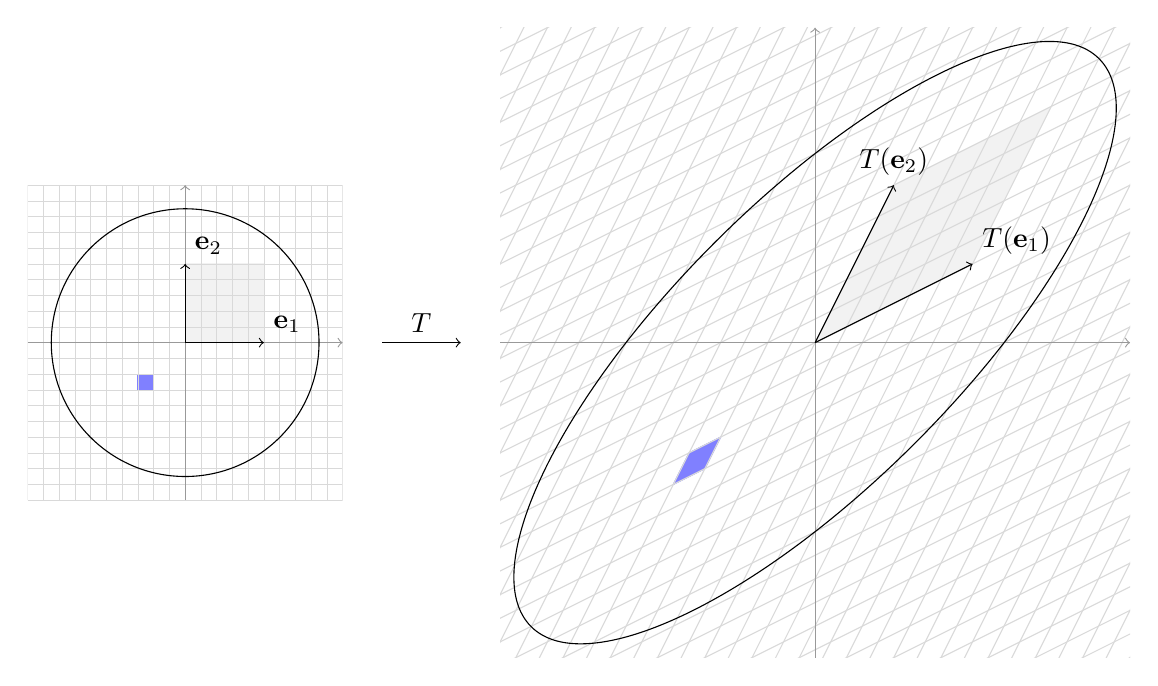
\begin{tikzpicture}
\def\XMAX{2};\def\YMAX{2};
\begin{scope}[xshift=-5cm]
\draw[color=blue!50,fill] (-0.6,-0.6)--(-0.6,-0.4)--(-0.4,-0.4)--(-0.4,-0.6)--cycle;
\draw[color=gray!10,fill] (0,0)--(1,0)--(1,1)--(0,1)--cycle;
\clip (-\XMAX,-\YMAX) rectangle (\XMAX,\YMAX);
\draw[help lines, color=gray!30, step=0.2] (-\XMAX,-\YMAX) grid (\XMAX,\YMAX);
\draw[->, color=gray!80] (-\XMAX,0)--(\XMAX,0) node[right]{$x_1$};
\draw[->, color=gray!80] (0,-\YMAX)--(0,\YMAX) node[above]{$x_2$};
\coordinate (e1) at (1,0); \node at (e1)[above right]{$\mathbf e_1$}; \draw[->] (0,0)--(e1);
\coordinate (e2) at (0,1); \node at (e2)[above right]{$\mathbf e_2$}; \draw[->] (0,0)--(e2);
\draw (0,0) circle (1.7);
\end{scope}
\draw[->](-2.5,0)--(-1.5,0);
\node at (-2,0)[above] {$T$};
\begin{scope}[xshift=3cm]
\draw[color=blue!50,fill] (-1.8,-1.8)--(-1.6,-1.4)--(-1.2,-1.2)--(-1.4,-1.6)--cycle;
\draw[color=gray!10,fill] (0,0)--(2,1)--(3,3)--(1,2)--cycle;
\clip (-2*\XMAX,-2*\YMAX) rectangle (2*\XMAX,2*\YMAX);
\foreach \i in {-4,-3.8,...,4}{
\draw[->, color=gray!30] (-10+\i,-5+2*\i)--(10+\i,5+2*\i);
\draw[->, color=gray!30] (-5+2*\i,-10+\i)--(5+2*\i,10+\i);
}
\draw[->, color=gray!80] (-2*\XMAX,0)--(2*\XMAX,0) node[right]{$x_1$};
\draw[->, color=gray!80] (0,-2*\YMAX)--(0,2*\YMAX) node[above]{$x_2$};
\coordinate (v1) at (2,1); \node at (v1)[above right]{$T(\mathbf e_1)$}; \draw[->] (0,0)--(v1);
\coordinate (v2) at (1,2); \node at (v2)[above]{$T(\mathbf e_2)$}; \draw[->] (0,0)--(v2);
\draw[rotate=45] (0,0) ellipse (5.1 and 1.8);
\end{scope}
\end{tikzpicture}
\end{center}
Since every small blue squares has been deformed into small parallelograms which are congruent to the gray square, parallelogram respectively and are of the same (signed) ratio $\det A$, so any area gets scaled by $\det A=2\cdot2-1\cdot1=3$ under $T$.
\end{answer}

\begin{remark}
In multi-variable calculus, this is known as the \textcolor{blue}{Jacobian}.
\end{remark}

\begin{theorem}
Suppose $A,B$ are $n\times n$ matrices, then $\det(AB)=(\det A)(\det B)$
\end{theorem}

\begin{proof}
Suppose $T_1,T_2$ are linear transformations with standard matrices $A,B$, respectively. Consider $T_2\circ T_1$ which should scale area by $\det(BA)$. On the other hand, this should scale area by $\det A$ and then $\det B$
\end{proof}

\begin{theorem}
$A$ is invertible $\iff\det A\neq0$. In addition, $\det(A^{-1})=\dfrac{1}{\det A}$.
\end{theorem}

\begin{proof}
If $A$ is invertible, then $A^{-1}$ is well-defined, then $1=\det I=\det(AA^{-1})=(\det A)(\det(A^{-1}))\Rightarrow \det(A^{-1})=\dfrac{1}{\det A}$, so $\det A\neq0$. Conversely, if $\det A\neq0$, $A$ would have $n$ pivots, so a pivot in each row and column, thus $A$ will be invertible.
\end{proof}

\begin{exercise}
Compute the determinants of the following matrices
\begin{itemize}
\item $\begin{bmatrix}
1&-2\\4&3
\end{bmatrix}$
\item $\begin{bmatrix}
1&5&-4\\
-1&-4&5\\
-2&-8&7
\end{bmatrix}$
\item $\begin{bmatrix}
0&0&0&1\\
0&2&0&3\\
0&7&-1&-8\\
2&2&-5&1
\end{bmatrix}$
\end{itemize}
\end{exercise}

\subsection{Cofactor expansion}

There is one more property of determinants. $\det\begin{bmatrix}
\mathbf w&\mathbf u+\mathbf v
\end{bmatrix}=\det\begin{bmatrix}
\mathbf w&\mathbf u
\end{bmatrix}+\det\begin{bmatrix}
\mathbf w&\mathbf v
\end{bmatrix}$

\begin{center}
\begin{tikzpicture}[scale=1]
\def\XMAX{2.5};\def\YMAX{2.5};
\draw[help lines, color=gray!30, dashed] (-\XMAX,-\YMAX) grid (\XMAX,\YMAX);
\draw[->, color=gray!80] (-\XMAX,0)--(\XMAX,0) node[right]{$x_1$};
\draw[->, color=gray!80] (0,-\YMAX)--(0,\YMAX) node[above]{$x_2$};
\coordinate (o) at (0,0);
\coordinate (w) at (1,0); \draw[->] (o)--(w)node[below right]{$\mathbf w$};
\coordinate (u) at (1,1); \draw[->,blue] (o)--(u)node[above right]{$\mathbf u$};
\coordinate (v) at (-0.5,1); \draw[->,red] (o)--($(u)+(v)$)node[above]{$\mathbf v$};
\draw[dashed,blue] (u)--($(u)+(w)$)--(w);
\draw[dashed,blue] ($(u)+(v)$)--(u)--($(u)+(w)$)--($(u)+(w)+(v)$)--cycle;
\draw[dashed,red] ($(u)+(v)$)--($(u)+(w)+(v)$)--(w);
\end{tikzpicture}
\end{center}

\begin{definition}
We use $a_{ij}$ to be denote the $(i,j)$-th entry of the matrix $A$, and $A_{ij}$ to denote the submatrix of $A$ by deleting the $i$-th row and the $j$-th column
\begin{center}
\begin{tikzpicture}
% \def\XMAX{2.5};\def\YMAX{2.5};\def\ZMAX{4.5};
% \mygrid{(-\XMAX,-\YMAX)}{(\XMAX,\YMAX)}{(0,0)};
\node at (0,0) {$\begin{bmatrix}
&&&&&\\
&&&&&\\
&&&&&\\
&&a_{ij}&&\\
&&&&&\\
&&&&&
\end{bmatrix}$};
\node at (-1.8,-0.2)[left] {$i$-th row}; \draw[->] (-1.8,-0.2)--(-1.4,-0.2);
\node at (-0.2,1.8)[above] {$j$-th column}; \draw[->] (-0.2,1.8)--(-0.2,1.4);
\end{tikzpicture}
\begin{tikzpicture}
% \def\XMAX{2.5};\def\YMAX{2.5};\def\ZMAX{4.5};
% \mygrid{(-\XMAX,-\YMAX)}{(\XMAX,\YMAX)}{(0,0)};
\node at (0,0) {$A_{ij}=\begin{bmatrix}
&&&&&\\
&&&&&\\
&&&&&\\
&&\,\,\,\,\,\,\,&&&\\
&&&&&\\
&&&&&
\end{bmatrix}$};
\draw[fill=black] (-0.7,-0.3)--(1.7,-0.3)--(1.7,-0.1)--(-0.7,-0.1)--cycle;
\draw[fill=black] (0.2,-1.3)--(0.4,-1.3)--(0.4,1.3)--(0.2,1.3)--cycle;
\end{tikzpicture}
\end{center}
We define the \textcolor{blue}{$(i,j)$-cofactor}\index{cofactor} to be $C_{ij}=(-1)^{i+j}\det A_{ij}$ (we also call $\det A_{ij}$ a \textcolor{blue}{minor}\index{minor}).
\end{definition}

For $n\geq2$, with the help of Lemma~\ref{lemma: det A lemma}, we derive cofactor expansion formula.

The \textcolor{blue}{cofactor expansion}\index{cofactor expansion} across the $i$-th row is
\[
\det A=a_{i1}C_{i1}+a_{i2}C_{i2}+\cdots+a_{in}C_{in}
\]
The cofactor expansion across the $j$-th column is
\[
\det A=a_{1j}C_{1j}+a_{2j}C_{2j}+\cdots+a_{nj}C_{nj}
\]
\begin{center}
\begin{tikzpicture}
\node at (-2,0) {$\begin{bmatrix}
\\
\\
\\
a_{i1}&a_{i2}&\cdots &a_{in}\\
\\
\\
\end{bmatrix}$};
\node at (2,0) {$\begin{bmatrix}
&&a_{1j}&&&\\
&&a_{2j}&&&\\
&&\vdots&&&\\
&&a_{nj}&&&\\
\end{bmatrix}$};
\end{tikzpicture}
\end{center}

\begin{proof}[Proof of Theorem~\ref{13:33-06/16/2022}]
Note that row cofactor expansion of $A$ is the same as column cofactor expansion of $A^T$. Hence we can prove this inductively on the size of the matrix.
\end{proof}

\begin{example}
\begin{align*}
&\left|\begin{matrix}
1&2&3&0\\
0&3&-1&0\\
-1&2&1&2\\
2&-3&1&0
\end{matrix}\right|\xequal{\text{cofactor expansion across last column}}2(-1)^{3+4}\left|\begin{matrix}
1&2&3\\
0&3&-1\\
2&-3&1
\end{matrix}\right|\\
&\xequal{R3\rightarrow R3-2R1}(-2)\left|\begin{matrix}
1&2&3\\
0&3&-1\\
0&-7&-5
\end{matrix}\right|\xequal{\text{cofactor expansion across first column}}(-2)\cdot1(-1)^{1+1}\left|\begin{matrix}
3&-1\\
-7&-5
\end{matrix}\right|\\
&=(-2)(3(-5)-(-1)(-7))=44
\end{align*}
\end{example}

\begin{remark}
When use the cofactor expansion, we want to apply it to rows/columns with more 0's
\end{remark}

\begin{exercise}
Suppose $A=\begin{bmatrix}
1&-1&1\\
2&0&-1\\
1&1&1\\
\end{bmatrix}$. Please find the cofactor expansion of $A$ across the
\begin{tasks}(2)
\task 1st row
\task 2nd column
\end{tasks}
And evaluate determinant of $A$.
\end{exercise}

\begin{solution}
\begin{align*}
\det A&=a_{11}C_{11}+a_{12}C_{12}+a_{13}C_{13}\\
&=a_{11}(-1)^{1+1}\det A_{11}+a_{12}(-1)^{1+2}\det A_{12}+a_{13}(-1)^{1+3}\det A_{13}\\
&=1\cdot(-1)^{1+1}\left|\begin{matrix}
0&-1\\1&1
\end{matrix}\right|+(-1)\cdot(-1)^{1+2}\left|\begin{matrix}
2&-1\\1&1
\end{matrix}\right|+1\cdot(-1)^{1+3}\left|\begin{matrix}
2&0\\1&1
\end{matrix}\right|\\
&=1\cdot(0\cdot1-(-1)\cdot1)+(-1)\cdot(2\cdot1-(-1)\cdot1)+1\cdot(-1)(2\cdot1-(-1)\cdot1)\\
&=6
\end{align*}
\begin{align*}
\det A&=a_{12}C_{12}+a_{22}C_{22}+a_{32}C_{32}\\
&=a_{11}(-1)^{1+1}\det A_{11}+a_{12}(-1)^{1+2}\det A_{12}+a_{13}(-1)^{1+3}\det A_{13}\\
&=(-1)\cdot(-1)^{1+2}\left|\begin{matrix}
2&-1\\1&1
\end{matrix}\right|+0\cdot(-1)^{2+2}\left|\begin{matrix}
1&1\\1&1
\end{matrix}\right|+1\cdot(-1)^{3+2}\left|\begin{matrix}
1&1\\2&-1
\end{matrix}\right|\\
&=(-1)\cdot(-1)(2\cdot1-(-1)\cdot1)+0\cdot(1\cdot1-1\cdot1)+1\cdot(-1)(1\cdot(-1)-1\cdot2)\\
&=6
\end{align*}
\end{solution}

\begin{exercise}
Suppose $A=\begin{bmatrix}
1&2&1\\
1&0&-1\\
-1&2&1
\end{bmatrix}$. Write out the cofactor expansion of $A$ across the second row, and evaluate the determinant $\det A$.
\end{exercise}

\begin{solution}
\begin{align*}
\det A&=a_{21}C_{21}+a_{22}C_{22}+a_{23}C_{23}\\
&=a_{21}(-1)^{2+1}\det A_{21}+a_{22}(-1)^{2+2}\det A_{22}+a_{23}(-1)^{2+3}\det A_{23}\\
&=1\cdot(-1)^{2+1}\left|\begin{matrix}
2&1\\2&1
\end{matrix}\right|+0\cdot(-1)^{2+2}\left|\begin{matrix}
1&1\\-1&1
\end{matrix}\right|+(-1)\cdot(-1)^{2+3}\left|\begin{matrix}
2&1\\2&1
\end{matrix}\right|\\
&=1\cdot(-1)(2\cdot1-1\cdot2)+0\cdot(1\cdot1-1\cdot(-1))+(-1)\cdot(-1)(1\cdot2-2\cdot(-1))\\
&=4
\end{align*}
\end{solution}

\begin{remark}
The REF of a square matrix $A$ is upper triangular, and $\det A=0$ if $A$ has less then $n$ pivots.
\end{remark}

\begin{exercise}
Suppose $A=\begin{bmatrix}
2&-1&3&1\\
0&-2&0&-1\\
0&0&3&1\\
0&0&0&1
\end{bmatrix}$. Please find use cofactor expansion  to find the $\det A$
\end{exercise}

\begin{solution}
Note that $A$ is upper triangular, so we could do cofactor expansions across first columns multiple times
\begin{align*}
\left|\begin{matrix}
2&-1&3&1\\
0&-2&0&-1\\
0&0&3&1\\
0&0&0&1
\end{matrix}\right|=2(-1)^{1+1}\left|\begin{matrix}
-2&0&-1\\
0&3&1\\
0&0&1
\end{matrix}\right|=2\cdot(-2)(-1)^{1+1}\left|\begin{matrix}
3&1\\
0&1
\end{matrix}\right|=2\cdot(-2)\cdot3\cdot(-1)^{1+1}1=-12
\end{align*}
\end{solution}

\begin{exercise}
Consider $A=\begin{bmatrix}
a&b\\c&d
\end{bmatrix}$. What is $A_{11},A_{12},A_{21},A_{22}$? What is $C_{11},C_{12},C_{21},C_{22}$. Write down the cofactor expansion of $A$ across the
\begin{itemize}
\item 1st row
\item 2nd row
\item 1st column
\item 2nd column
\end{itemize}
\end{exercise}

\begin{solution}
$A_{11}=[d],A_{12}=[c],A_{21}=[b],A_{22}=[a]$ are all 1 by 1 matrices. $C_{11}=(-1)^{1+1}\det A_{11}=d,C_{12}=(-1)^{1+2}\det A_{21}=-c,C_{21}=(-1)^{2+1}\det A_{21}=-b,C_{22}=(-1)^{2+2}\det A_{22}=a$. So the cofactor expansions are
\begin{itemize}
\item $\det A=aC_{11}+bC_{12}=ad-bc$
\item $\det A=cC_{21}+dC_{22}=-bc+ad$
\item $\det A=aC_{11}+cC_{21}=ad-bc$
\item $\det A=bC_{12}+dC_{22}=-bc+ad$
\end{itemize}
Note that all of the above calculations show that $\det A=\det\begin{bmatrix}
a&b\\c&d
\end{bmatrix}=ad-bc$.
\end{solution}

\section{Lecture 9 - Vector spaces and subspaces}

\subsection{Vector space}

To motivate the definition of a vector space, let's consider the following example

\begin{example}\label{17:45-06/27/2022}
Let $\mathbb P_n$ denote the set of (real) polynomials of degree less or equal to $n$. For example $\mathbb P_0=\mathbb R$ is just the set of real numbers, and
\begin{align*}
\mathbb P_1&=\{a_0+a_1t|a_0,a_1\in\mathbb R\} \\
\mathbb P_2&=\{a_0+a_1t+a_2t^2|a_0,a_1,a_2\in\mathbb R\}\\
\mathbb P_3&=\{a_0+a_1t+a_2t^2+a_3t^3|a_0,a_1,a_2,a_3\in\mathbb R\}\\
&\vdots\\
\mathbb P_n&=\{a_0+a_1t+a_2t^2+\cdots+a_nt^n|a_0,a_1,a_2,\cdots,a_n\in\mathbb R\}.
\end{align*}
You may soon realize that $\mathbb P_n$ can be identified with $\mathbb R^{n+1}$.
\begin{center}
\begin{tikzcd}
\mathbb P_1 \arrow[r,equal,"\sim"]        & \mathbb R^2   \\
\{a_0+a_1t\} \arrow[r, leftrightsquigarrow] \arrow[u, equal] & \left\{\begin{bmatrix}a_0\\a_1\end{bmatrix}\right\} \arrow[u, equal]
\end{tikzcd}
\begin{tikzcd}
\mathbb P_2 \arrow[r,equal,"\sim"]        & \mathbb R^3\\
\{a_0+a_1t+a_2t^2\} \arrow[r, leftrightsquigarrow] \arrow[u, equal] & \left\{\begin{bmatrix}a_0\\a_1\\a_2\end{bmatrix}\right\} \arrow[u, equal]
\end{tikzcd}
\begin{tikzcd}
\mathbb P_n \arrow[r,equal,"\sim"]        & \mathbb R^{n+1}          \\
\{a_0+a_1t+a_2t^2+\cdots+a_nt^n\} \arrow[r, leftrightsquigarrow] \arrow[u, equal] & \left\{\begin{bmatrix}a_0\\a_1\\\vdots\\a_n\end{bmatrix}\right\} \arrow[u, equal]
\end{tikzcd}
\end{center}
More concrete examples could be
\begin{enumerate}
\item For $\mathbb P_1\cong\mathbb R^2$, $1+2t\leftrightsquigarrow\begin{bmatrix}
1\\2
\end{bmatrix}$
\item For $\mathbb P_2\cong\mathbb R^3$, $3t^2-1\leftrightsquigarrow\begin{bmatrix}
-1\\0\\3
\end{bmatrix}$
\end{enumerate}
If we consider addition and scalar multiplication, we have
\begin{center}
\begin{tikzpicture}
\tikzset{<-squig->/.style={to-to, decorate, decoration={zigzag,segment length=5,amplitude=1,pre=lineto,post=lineto,post length=2pt,pre length=2pt}}}
\node at (0,1) {$\begin{bmatrix}
1\\0\\2
\end{bmatrix}+\begin{bmatrix}
2\\1\\0
\end{bmatrix}=\begin{bmatrix}
3\\1\\2
\end{bmatrix}$};
\node at (0,-1) {$(1+2t^2)+(2+t)=3+t+2t^2$};
\draw[<-squig->] (-1.1,0.2)--(-1.8,-0.7);
\draw[<-squig->] (0,0.2)--(-0.1,-0.7);
\draw[<-squig->] (1.1,0.2)--(1.5,-0.7);
\end{tikzpicture}
\qquad
\begin{tikzpicture}
\tikzset{<-squig->/.style={to-to, decorate, decoration={zigzag,segment length=5,amplitude=1,pre=lineto,post=lineto,post length=2pt,pre length=2pt}}}
\node at (0,1) {$2\cdot\begin{bmatrix}
1\\0\\2
\end{bmatrix}=\begin{bmatrix}
2\\0\\4
\end{bmatrix}$};
\node at (0,-1) {$2\cdot(1+2t^2)=2+4t^2$};
\draw[<-squig->] (-0.35,0.2)--(-0.6,-0.7);
\draw[<-squig->] (0.8,0.2)--(1.1,-0.7);
\end{tikzpicture}
\end{center}
So we may conclude that addition and scalar multiplication in $\mathbb P_n$ can be identically translated to addition and scalar multiplication in $\mathbb R^{n+1}$
\end{example}

\begin{remark}
We call $\{1,t,t^2,\cdots,t^n\}$ the \textit{standard basis} of $\mathbb P_n$, corresponding to the standard basis for $\mathbb R^{n+1}$
\end{remark}

\begin{example}
$\left\{1,t,t^2\right\}$ is the standard basis for $\mathbb P_2$, and
\begin{align*}
p(t)&=a_0+a_1t+a_2t^2=a_0\cdot 1+a_1\cdot t+a_2\cdot t^2
\end{align*}
\end{example}

\begin{example}\label{17:53-06/27/2022}
Let's denote $M_{m\times n}(\mathbb R)$ the set of $m\times n$ matrices. For example
\begin{align*}
M_{2\times2}(\mathbb R)&=\left\{\begin{bmatrix}
a_{11}&a_{12}\\
a_{21}&a_{22}
\end{bmatrix}\middle|a_{11},a_{12},a_{21},a_{22}\in\mathbb R\right\}\\
M_{3\times2}(\mathbb R)&=\left\{\begin{bmatrix}
a_{11}&a_{12}\\
a_{21}&a_{22}\\
a_{31}&a_{32}
\end{bmatrix}\middle|a_{11},a_{12},a_{21},a_{22},a_{31},a_{32}\in\mathbb R\right\}\\
M_{2\times3}(\mathbb R)&=\left\{\begin{bmatrix}
a_{11}&a_{12}&a_{13}\\
a_{21}&a_{22}&a_{23}
\end{bmatrix}\middle|a_{11},a_{12},a_{13},a_{21},a_{22},a_{23}\in\mathbb R\right\}\\
&\vdots\\
M_{m\times n}(\mathbb R)&=\left\{\begin{bmatrix}
a_{11}&a_{12}&\cdots&a_{1n}\\
a_{21}&a_{22}&\cdots&a_{2n}\\
\vdots&\vdots&&\vdots\\
a_{m1}&a_{m2}&\cdots&a_{mn}\\
\end{bmatrix}\middle|a_{11},\cdots,a_{1n},\cdots,a_{m1},\cdots,a_{mn}\in\mathbb R\right\}.
\end{align*}
You may realize that $M_{m\times n}(\mathbb R)$ can be identified with $\mathbb R^{mn}$
\begin{center}
\begin{tikzcd}
M_{2\times 2}(\mathbb R) \arrow[r,equal,"\sim"]        & \mathbb R^{4}   \\
\left\{\begin{bmatrix}
a_{11}&a_{12}\\
a_{21}&a_{22}
\end{bmatrix}\right\} \arrow[r, leftrightsquigarrow] \arrow[u, equal] & \left\{\begin{bmatrix}a_{11}\\a_{12}\\a_{21}\\a_{22}\end{bmatrix}\right\} \arrow[u, equal]
\end{tikzcd}
\begin{tikzcd}
M_{3\times 2}(\mathbb R) \arrow[r,equal,"\sim"]        & \mathbb R^{6}   \\
\left\{\begin{bmatrix}
a_{11}&a_{12}\\
a_{21}&a_{22}\\
a_{31}&a_{32}
\end{bmatrix}\right\} \arrow[r, leftrightsquigarrow] \arrow[u, equal] & \left\{\begin{bmatrix}a_{11}\\a_{12}\\a_{21}\\a_{22}\\a_{31}\\a_{32}\end{bmatrix}\right\} \arrow[u, equal]
\end{tikzcd}
\begin{tikzcd}
M_{2\times 3}(\mathbb R) \arrow[r,equal,"\sim"]        & \mathbb R^{6}   \\
\left\{\begin{bmatrix}
a_{11}&a_{12}&a_{13}\\
a_{21}&a_{22}&a_{23}
\end{bmatrix}\right\} \arrow[r, leftrightsquigarrow] \arrow[u, equal] & \left\{\begin{bmatrix}a_{11}\\a_{12}\\a_{13}\\a_{21}\\a_{22}\\a_{23}\end{bmatrix}\right\} \arrow[u, equal]
\end{tikzcd}
\begin{tikzcd}
M_{m\times n}(\mathbb R) \arrow[r,equal,"\sim"]        & \mathbb R^{mn}   \\
\left\{\begin{bmatrix}
a_{11}&a_{12}&\cdots&a_{1n}\\
a_{21}&a_{22}&\cdots&a_{2n}\\
\vdots&\vdots&&\vdots\\
a_{m1}&a_{m2}&\cdots&a_{mn}\\
\end{bmatrix}\right\} \arrow[r, leftrightsquigarrow] \arrow[u, equal] & \left\{\begin{bmatrix}a_{11}\\\vdots\\a_{1n}\\\vdots\\a_{m1}\\\vdots\\a_{mn}\end{bmatrix}\right\} \arrow[u, equal]
\end{tikzcd}
\end{center}
In more concrete terms, addition and scalar multiplication can be identified as the following
\begin{center}
\begin{tikzpicture}
\tikzset{<-squig->/.style={to-to, decorate, decoration={zigzag,segment length=5,amplitude=1,pre=lineto,post=lineto,post length=2pt,pre length=2pt}}}
\node at (0,1) {$\begin{bmatrix}
1&0\\1&1
\end{bmatrix}+\begin{bmatrix}
-1&0\\2&3
\end{bmatrix}=\begin{bmatrix}
0&0\\4&6
\end{bmatrix}$};
\node at (0,-1) {$\begin{bmatrix}
1\\0\\1\\1
\end{bmatrix}+\begin{bmatrix}
-1\\0\\2\\3
\end{bmatrix}=\begin{bmatrix}
0\\0\\4\\6
\end{bmatrix}$};
\draw[<-squig->] (-1.6,0.5)--(-1.2,-0.1);
\draw[<-squig->] (0,0.5)--(0,-0.1);
\draw[<-squig->] (1.6,0.5)--(1.2,-0.1);
\end{tikzpicture}
\qquad
\begin{tikzpicture}
\tikzset{<-squig->/.style={to-to, decorate, decoration={zigzag,segment length=5,amplitude=1,pre=lineto,post=lineto,post length=2pt,pre length=2pt}}}
\node at (0,1) {$2\cdot\begin{bmatrix}
-1&0\\2&3
\end{bmatrix}=\begin{bmatrix}
-2&0\\4&6
\end{bmatrix}$};
\node at (0,-1) {$2\cdot\begin{bmatrix}
-1\\0\\2\\3
\end{bmatrix}=\begin{bmatrix}
-2\\0\\4\\6
\end{bmatrix}$};
\draw[<-squig->] (-0.6,0.5)--(-0.5,-0.1);
\draw[<-squig->] (1.1,0.5)--(0.9,-0.1);
\end{tikzpicture}
\end{center}
So we may conclude that addition and scalar multiplication in $M_{m\times n}(\mathbb R)$ can be identically translated to addition and scalar multiplication in $\mathbb R^{mn}$
\end{example}

\begin{remark}
We call $\{E_{ij}\}$ the \textit{standard basis} of $M_{m\times n}(\mathbb R)$, corresponding to the standard basis for $\mathbb R^{mn}$. Here $E_{ij}$ is the $m\times n$ matrix that only has a single 1 in the $(i,j)$-th spot, but 0's elsewhere.
\end{remark}

\begin{example}
$\left\{E_{11}=\begin{bmatrix}
1&0\\0&0
\end{bmatrix},E_{12}=\begin{bmatrix}
0&1\\0&0
\end{bmatrix},E_{21}=\begin{bmatrix}
0&0\\1&0
\end{bmatrix},E_{22}=\begin{bmatrix}
0&0\\0&1
\end{bmatrix}\right\}$ is the standard basis for $M_{2\times2}(\mathbb R)$, and
\begin{align*}
\begin{bmatrix}
a_{11}&a_{12}\\a_{21}&a_{22}
\end{bmatrix}&=\begin{bmatrix}
a_{11}&0\\0&0
\end{bmatrix}+\begin{bmatrix}
0&a_{12}\\0&0
\end{bmatrix}+\begin{bmatrix}
0&0\\a_{21}&0
\end{bmatrix}+\begin{bmatrix}
0&0\\0&a_{22}
\end{bmatrix}\\
&=a_{11}\begin{bmatrix}
1&0\\0&0
\end{bmatrix}+a_{12}\begin{bmatrix}
0&1\\0&0
\end{bmatrix}+a_{21}\begin{bmatrix}
0&0\\1&0
\end{bmatrix}+a_{22}\begin{bmatrix}
0&0\\0&1
\end{bmatrix}\\
&=a_{11}E_{11}+a_{12}E_{12}+a_{21}E_{21}+a_{22}E_{22}
\end{align*}
\end{example}

\begin{definition}
A \textcolor{blue}{(real) vector space}\index{vector space} is a set $V$ of objects, called \textit{vectors}, on which are defined two operations, called \textit{addition} $\fatplus$ and \textit{(left) scalar multiplication} $\fatdot$, subject to axioms
\begin{enumerate}\setcounter{enumi}{-1}
\item $\bm u\fatplus\bm v$ and $c\fatdot\bm v$ are still in $V$
\item $\bm u\fatplus\bm v=\bm v\fatplus\bm u$
\item $(\bm u\fatplus\bm v)\fatplus\bm w=\bm u\fatplus(\bm v\fatplus\bm w)$
\item There is a \textit{zero vector} $\bm 0$ such that $\bm u\fatplus\bm 0=\bm u$
\item For each $\bm u$ in $V$, there is a vector $\fatminus\bm u$ in $V$ such that $\bm u\fatplus(\fatminus\bm u)=\bm 0$
\item $c\fatdot(\bm u\fatplus\bm v)=c\fatdot\bm u\fatplus c\fatdot\bm v$
\item $(c+d)\fatdot\bm u=c\fatdot\bm u\fatplus d\fatdot\bm u$
\item $c\fatdot(d\fatdot\bm u)=(cd)\fatdot\bm u$
\item $1\fatdot\bm u=\bm u$
\end{enumerate}
\end{definition}

\begin{example}
Set $V$ to be $\mathbb R^n$, $\fatplus$ to be addition $+$ for vectors, $\fatdot$ to be scalar multiplication $\cdot$ for vectors, then this is a vector space
\end{example}

\begin{example}[non-example]
Suppose $V=\mathbb R$, $a\fatplus b=a+b+1$, $c\fatdot a=c\cdot a=ca$, we can check
\begin{enumerate}\setcounter{enumi}{-1}
\item $a\fatplus b=a+b+1\in\mathbb R$, $c\fatdot a=ca\in\mathbb R$
\item $a\fatplus b=a+b+1=b+a+1=b\fatplus a$
\item $(a\fatplus b)\fatplus c=(a+b+1)+c+1=a+(b+c+1)+1=a\fatplus(b\fatplus c)$
\item There is a \textit{zero vector} $\bm 0=-1$ such that $a\fatplus\bm 0=a+(-1)+1=a$
\item For each $a$, we have $\fatminus a=-a-2$ such that $a\fatplus(\fatminus a)=a+(-a-2)+1=-1=\bm 0$
\end{enumerate}
However $2\fatdot(a\fatplus b)=2(a+b+1)\neq 2a+2b+1=2\fatdot a\fatplus 2\fatdot b$. Therefore, this is not a vector space
\end{example}

\subsection{Subspace}

\begin{definition}
Suppose $V$ is a vector space with addition $\fatplus$ and scalar multiplication $\fatdot$. A \textcolor{blue}{subspace}\index{subspace} $H$ is a non-empty subset which closed under addition and scalar multiplication, i.e. for any $\bm u,\bm v\in H$, $c\in\mathbb R$, $\bm u\fatplus\bm v,c\fatdot\bm u\in H$
\end{definition}

\begin{remark}
It is easy to check that a subspace $H$ is again a vector space.
\end{remark}

\begin{exercise}\label{17:08-06/29/2022}
Recall that $M_{2\times2}(\mathbb R)$ is the set of 2 by 2 matrices, and that a square matrix $A$ is \textit{symmetric} if $A^T=A$. Consider a subset $V$ consists of 2 by 2 symmetric matrices, i.e. $V=\left\{A\in M_{2\times2}(\mathbb R)\middle|A^T=A\right\}$
\begin{enumerate}
\item Show that $V$ is a vector space.
\item Find a basis for $V$.
\end{enumerate}
\end{exercise}

\begin{solution}
\begin{enumerate}
\item For any $A,B\in V$, $c\in\mathbb R$, by definition we know that $A^T=A$, $B^T=B$, we want to show that $A+B\in V$, $cA\in V$ (condition for subspace), i.e. $(A+B)^T=A^T+B^T$, $(cA)^T=cA$. This is true because
\[
(A+B)^T=A^T+B^T=A+B,\qquad (cA)^T=cA^T=cA
\]
Therefore $V$ is a subspace of $M_{2\times2}(\mathbb R)$, and thus a vector space
\item Suppose $A=\begin{bmatrix}
a_{11}&a_{12}\\a_{21}&a_{22}
\end{bmatrix}\in M_{2\times2}(\mathbb R)$, then $a_{12}=a_{21}$, so we may conclude that
\[
V=\left\{\begin{bmatrix}
a&b\\b&c
\end{bmatrix}\in M_{2\times2}(\mathbb R)\middle|a,b,c\in\mathbb R\right\}
\]
Note that
\begin{equation}\label{17:01-06/24/2022}
\begin{aligned}
\begin{bmatrix}
a&b\\b&c
\end{bmatrix}=\begin{bmatrix}
a&0\\0&0
\end{bmatrix}+\begin{bmatrix}
0&b\\b&0
\end{bmatrix}+\begin{bmatrix}
0&0\\0&c
\end{bmatrix}=a\begin{bmatrix}
1&0\\0&0
\end{bmatrix}+b\begin{bmatrix}
0&1\\1&0
\end{bmatrix}+c\begin{bmatrix}
0&0\\0&1
\end{bmatrix}
\end{aligned}
\end{equation}
And that linear combination~\eqref{17:01-06/24/2022} is the zero matrix $\iff a=b=c=0$, thus $\mathcal B=\left\{\begin{bmatrix}
1&0\\0&0
\end{bmatrix},\begin{bmatrix}
0&1\\1&0
\end{bmatrix},\begin{bmatrix}
0&0\\0&1
\end{bmatrix}\right\}$ is a basis for $V$
\end{enumerate}
\end{solution}

\begin{exercise}\label{ker T for T take sum of coef of poly}
Suppose $H=\{p(t)=a_0+a_1t+a_2t^2\in\mathbb P_2|a_0+a_1+a_2=0\}$ is the set of polynomials of degree $\leq 2$ and sum of coefficients zero. Show that $H$ is a vector space.
\end{exercise}

\begin{example}\label{15:10-06/23/2022}
Consider the vector space $V=\mathbb R^2$, and $H$ is the set of solutions to the linear equation $2x_1-x_2+2=0$, then $H$ is not a subspace. For example, if we choose $\mathbf u=\begin{bmatrix}
-1\\0
\end{bmatrix},\mathbf v=\begin{bmatrix}
0\\2
\end{bmatrix}$, then $\mathbf u+\mathbf v=\begin{bmatrix}
-1\\2
\end{bmatrix}$ is not in $H$, nor is $2\mathbf u=\begin{bmatrix}
-2\\0
\end{bmatrix}$
\begin{center}
\begin{tikzpicture}
\def\XMAX{2.5};\def\YMAX{2.5};\def\ZMAX{4.5};
\begin{scope}
\clip(-\XMAX,-\YMAX) rectangle (\XMAX,\YMAX);
\draw (-3,-4)--(3,8);
\draw[blue] (-3,-6)--(3,6);
\end{scope}
\draw[help lines, color=gray!30, dashed] (-\XMAX,-\YMAX) grid (\XMAX,\YMAX);
\draw[->, color=gray!80] (-\XMAX,0)--(\XMAX,0) node[right]{$x_1$};
\draw[->, color=gray!80] (0,-\YMAX)--(0,\YMAX) node[above]{$x_2$};
\coordinate (u) at (-1,0); \node at (u)[below right]{$\mathbf u$}; \draw[->,thick] (0,0)--(u);
\coordinate (v) at (0,2); \node at (v)[below right]{$\mathbf v$}; \draw[->,thick] (0,0)--(v);
\draw[->,thick,blue] (0,0)--(1,2);
\node at ($2*(u)$)[below right]{$2\mathbf u$}; \draw[->] (0,0)--($2*(u)$);
\node at ($(u)+(v)$)[below left]{$\mathbf u+\mathbf v$}; \draw[->] (0,0)--($(u)+(v)$);
% \draw[dashed] (u)--($(u)+(v)$); \draw[dashed] (v)--($(u)+(v)$);
\node at (-2,-2)[left] {$H$};
\node at (1,2)[below right] {$H_1$};
\end{tikzpicture}
\end{center}
The reason is that $H$ is not homogeneous. If we consider $H_1$ to be solution set of the homogeneous equation $2x_1-x_2=0$, we see that $H_1$ is a subspace as it is the span of a single vector $\begin{bmatrix}
1\\2
\end{bmatrix}$.
\end{example}

\section{Lecture 10 - Null spaces, Column spaces, Row spaces, Rank and Nullity}

\subsection{Null space, Column Space and Row space}

\begin{definition}
Suppose $V$ is a vector space, $\{\bm v_1,\bm v_2,\cdots,\bm v_n\}\subseteq V$ is a set of linearly independent vectors that span $V$, we define the \textcolor{blue}{dimension}\index{dimension} of $V$ to be $\dim V=n$.
\end{definition}

\begin{definition}
Suppose $A$ is a $m\times n$ matrix, we define the \textcolor{blue}{null space}\index{null space} of $A$ to be
\[
\Nul A=\{\mathbf x\in\mathbb R^n|A\mathbf x=\mathbf0\}=\text{solution set of $A\mathbf x=\mathbf 0$}
\]
Note that the solution set to linear system $A\mathbf x=\mathbf0$ is the intersection of $m$ hyperplanes (one for each homogeneous equation) that pass through the origin.
\end{definition}

\begin{example}
$A=\begin{bmatrix}
1&-3&2\\
-5&12&-1
\end{bmatrix}$, the to find the $\Nul A$ is equivalent to solve $A\mathbf x=\mathbf 0$
\begin{align*}
\begin{bmatrix}
A&\mathbf 0
\end{bmatrix}\xsim{R2\rightarrow R2+5R1}\begin{bmatrix}
1&-3&2&0\\
0&-3&9&0
\end{bmatrix}\xsim{R2/(-3)}\begin{bmatrix}
1&-3&2&0\\
0&1&-3&0
\end{bmatrix}\xsim{R1\rightarrow R1+3R2}\begin{bmatrix}
1&0&-7&0\\
0&1&-3&0
\end{bmatrix}
\end{align*}
Hence the solution set is $\begin{cases}
x_1=7x_3\\
x_2=3x_3\\
x_3\text{ is free}
\end{cases}$, in parametric form, $\begin{bmatrix}
x_1\\x_2\\x_3
\end{bmatrix}=x_3\begin{bmatrix}
7\\3\\1
\end{bmatrix}$, which describes a line in $\mathbb R^3$ of the direction $\begin{bmatrix}
7\\3\\1
\end{bmatrix}$ that passes through the origin, and this line is the intersection of planes $x_1-3x_2+2x_3=0$ and $-5x_1+12x_2-x_3=0$
\begin{center}
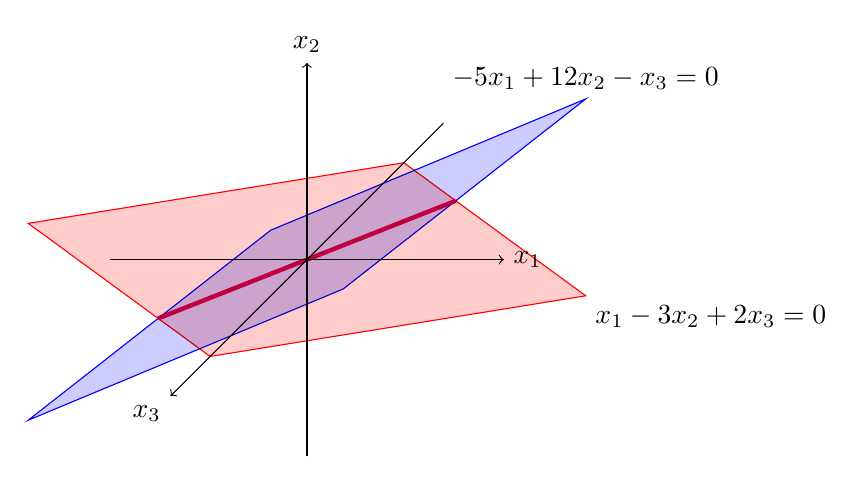
\begin{tikzpicture}
\definecolor{color1}{rgb}{255,0,0}
\definecolor{color2}{rgb}{0,0,255}
\definecolor{color3}{rgb}{255,0,255}
\def\XMAX{2.5};\def\YMAX{2.5};\def\ZMAX{4.5};
\begin{scope}[blend mode=multiply]
\draw [color1, fill=color1!20] plot (-2,-2,-2)--(-2,2,4)--(2,2,2)--(2,-2,-4)--cycle;
\node at (2,-2,-4) [below right]{$x_1-3x_2+2x_3=0$};
\draw [color2, fill=color2!20] plot (-2,-7/6,-4)--(-2,-1/2,4)--(2,7/6,4)--(2,1/2,-4)--cycle;
\node at (2,1/2,-4) [above]{$-5x_1+12x_2-x_3=0$};
\end{scope}
\draw [purple, ultra thick](-2,-6/7,-2/7)--(2,6/7,2/7);
\draw[->] (-\XMAX,0,0)--(\XMAX,0,0) node[right]{$x_1$};
\draw[->] (0,-\YMAX,0)--(0,\YMAX,0) node[above]{$x_2$};
\draw[->] (0,0,-\ZMAX)--(0,0,\ZMAX) node[below left]{$x_3$};
\end{tikzpicture}
\end{center}
\end{example}

\begin{remark}
As discussed in Example~\ref{15:10-06/23/2022}, in general, the solution set of $A\mathbf x=\mathbf b$ is not a subspace of $\mathbb R^n$ unless $\mathbf b=\mathbf0$. And in fact, any subspace of $\mathbb R^n$ is the null space for some $m\times n$ matrix $A$, i.e. the intersection of hyperplanes passing through the origin
\end{remark}

\begin{definition}
Suppose $A=\begin{bmatrix}
\mathbf a_1&\mathbf a_2&\cdots&\mathbf a_n
\end{bmatrix}$ is an $m\times n$ matrix, then the \textcolor{blue}{column space}\index{column space} (denote as $\Col A$) is the subspace $\Span\{\mathbf a_1,\mathbf a_2,\cdots,\mathbf a_n\}$ in $\mathbb R^m$. Suppose $A=\begin{bmatrix}
R1\\R2\\\vdots\\Rm
\end{bmatrix}$, then the \textcolor{blue}{row space}\index{row space} (denote as $\Row A$) is the subspace spaned by row vectors $\Span\{R1,R2,\cdots, Rm\}$ in $\mathbb R^n$ written horizontally.
\end{definition}

\begin{theorem}
Row reductions preserve $\Nul A, \Row A$, but not $\Col A$. However, row reductions preserve linear dependences of the column vectors.
\end{theorem}

\begin{remark}
Suppose $A\mathbf x=\mathbf0$ is some linear dependence of the column vectors of $A$, after elementary row reduction $A\sim EA$, $(EA)\mathbf x=E(A\mathbf x)=E\mathbf0=\mathbf0$ is again the same linear dependence of columns of $EA$. In other words, the linear dependence of columns of a matrix is preserved by row equivalence.
\end{remark}

\begin{theorem}
Suppose $A$ is a $m\times n$ matrix, $A\sim U$ is of RREF form
\begin{itemize}
\item The vectors in the parametric vector form of the solution set of $A\mathbf x=\mathbf0$ gives a basis for $\Nul A$. Note that $\dim\Nul A=$ the number of free variables.
\item A basis for $\Col A$ could be the set of pivot columns in $A$. Note that $\dim\Col A=$ the number of pivots.
\item A basis for $\Row A$ could be the set of non-zero row vectors in $U$ (Or any REF of $A$). Note that $\dim\Row A=$ the number of pivots.
\end{itemize}
\end{theorem}

\subsection{Rank and Nullity}

\begin{definition}
$\dim\Nul A$ is also name the \textcolor{blue}{nullity}\index{nullity} of $A$. The number of pivots of $A$ (which is equal to both $\dim\Col A$ and $\dim\Row A$) is called the \textcolor{blue}{rank}\index{rank} of $A$
\end{definition}

\begin{theorem}[Rank-Nullity theorem]\label{16:38-06/24/2022}
Notice that the number of columns in $A$ (say a $m\times n$ matrix) is equal to the number of free variables and the number of pivot columns, thus we have
\begin{center}
$n=$ nullity + rank
\end{center}
\end{theorem}

\begin{example}
$A=\begin{bmatrix}
1&-1&1\\
2&0&-1\\
1&1&-2
\end{bmatrix}\sim\begin{bmatrix}
1&-1&1\\
0&2&-3\\
0&0&0
\end{bmatrix}\sim\begin{bmatrix}
1&0&-\frac{1}{2}\\
0&1&-\frac{3}{2}\\
0&0&0
\end{bmatrix}$, which is an REF and an RREF respectively. There is only one free variable $x_3$, so the nullity is 1, and the 1st, 2nd columns are pivot columns, so the rank is 2. We see that Theorem~\ref{16:38-06/24/2022} holds as $3=1+2$, and
\[
\Nul A=\Span\left\{\begin{bmatrix}
\frac{1}{2}\\\frac{3}{2}\\1
\end{bmatrix}\right\}
\]
\[
\Col A=\Span\left\{\begin{bmatrix}
1\\2\\1
\end{bmatrix},\begin{bmatrix}
-1\\0\\1
\end{bmatrix}\right\}
\]
\[
\Row A=\Span\left\{\begin{bmatrix}
1&0&-\frac{1}{2}
\end{bmatrix},\begin{bmatrix}
0&1&-\frac{3}{2}
\end{bmatrix}\right\}\text{ or }\Span\left\{\begin{bmatrix}
1&-1&1
\end{bmatrix},\begin{bmatrix}
1&2&-3
\end{bmatrix}\right\}
\]
\end{example}

\begin{exercise}
$A=\begin{bmatrix}
1&2&0&4&5\\
0&0&5&-7&8\\
0&0&0&0&-9\\
0&0&0&0&0
\end{bmatrix}\sim\begin{bmatrix}
1&2&0&4&0\\
0&0&1&-\frac{7}{5}&0\\
0&0&0&0&1\\
0&0&0&0&0
\end{bmatrix}$
Note that here we have 2 free variables $x_2,x_4$, so the nullity is 2, and the 1st, 3rd, 5th columns are pivot columns, so the rank is 3. We see that Theorem~\ref{16:38-06/24/2022} holds as $5=2+3$, and
\[
\Nul A=\Span\left\{\begin{bmatrix}
-2\\1\\0\\0\\0
\end{bmatrix},\begin{bmatrix}
-4\\0\\\frac{7}{5}\\1\\
\end{bmatrix}\right\}
\]
\[
\Col A=\Span\left\{\begin{bmatrix}
1\\0\\0\\0
\end{bmatrix},\begin{bmatrix}
0\\5\\0\\0
\end{bmatrix},\begin{bmatrix}
5\\8\\-9\\0
\end{bmatrix}\right\}
\]
\[
\Row A=\Span\left\{\begin{bmatrix}
1&2&0&4&5
\end{bmatrix},\begin{bmatrix}
0&0&5&-7&8
\end{bmatrix},\begin{bmatrix}
0&0&0&0&-9
\end{bmatrix}\right\}
\]
\end{exercise}

\begin{question}
If you have a set $\mathcal S$ of vectors in $\mathbb R^m$, how do you find a subset of $\mathcal S$ that is a basis for $\Span\{\mathcal S\}$ (i.e. remove linear dependences)?
\end{question}

\begin{answer}
Collect these vectors as the column vectors of a matrix, and then find its columns space.
\end{answer}

\begin{exercise}
Suppose $\mathbf v_1=\begin{bmatrix}
1\\2\\1
\end{bmatrix}$, $\mathbf v_2=\begin{bmatrix}
-1\\0\\1
\end{bmatrix}$, $\mathbf v_3=\begin{bmatrix}
1\\-1\\-2
\end{bmatrix}$. Find a basis for $\Span\{\mathbf v_1, \mathbf v_2, \mathbf v_3\}$.
\end{exercise}

\begin{exercise}
Suppose $A=\begin{bmatrix}
1&-7&0&6&5\\
0&0&1&-2&-3\\
-1&7&-4&2&7
\end{bmatrix}$. Find $\Nul A,\Row A,\Col A$, and the nullity, rank of $A$.
\end{exercise}

\section{Lecture 11 - Linear transformations in general}

\subsection{Linear transformation}

\begin{definition}
Suppose $V,W$ are vector spaces, a \textit{linear transformation} is a mapping $T:V\to W$ such that
\begin{itemize}
\item $T(\bm u\fatplus\bm v)=T(\bm u)\fatplus T(\bm v)$
\item $T(c\fatdot u)=c\fatdot T(\bm u)$
\end{itemize}
Just as before, we call $V$ the \textit{domain} of $T$, $W$ the \textit{codomain} of $T$, the \textit{image} of $\bm x$ under $T$ is $T(\bm x)$, the set of images $\{T(\bm x)|\bm x\in V\}$ the \textit{range} (denoted as $\Range T$), and the set $\{\bm x|T(\bm x)=\bm b\}$ the preimage of $\bm b$ under $T$. We still say that $T$ is \textit{one-to-one} if any $\bm b\in W$, there is at most one $\bm x\in V$ such that $T(\bm x)=\bm b$. $T$ is \textit{onto} the range is the codomain. $T$ is said to be \textit{invertible} if $T$ has a inverse (this happens if and only if $T$ is both one-to-one and onto, and we can easily check that $T^{-1}$ is also an linear transformation), in this case we also call $T$ an \textcolor{blue}{isomorphism}\index{isomorphism}.
\end{definition}

\begin{definition}
We call $\{\bm x|T(\bm x)=\bm0\}$ the \textcolor{blue}{kernel}\index{kernel} (or \textcolor{blue}{null space}) of $T$, and denote it as $\ker T$.
\end{definition}

\begin{remark}\label{14:24/06/30/2022}
Suppose $T:\mathbb R^n\to\mathbb R^m$, $T(\mathbf x)=A\mathbf x$ is a matrix transformation, then $\ker T=\Nul A$, $\Range T=\Col A$
\end{remark}

\begin{example}
The identification
\[
T:\mathbb P_2\to\mathbb R^3,\qquad T(a_0+a_1t+a_2t^2)=\begin{bmatrix}
a_0\\a_1\\a_2
\end{bmatrix}
\]
in Eaxmple~\ref{17:45-06/27/2022} is an invertible linear transformation with inverse linear transformation
\[
T^{-1}:\mathbb R^3\to\mathbb P_2,\qquad T^{-1}\left(\begin{bmatrix}
a_0\\a_1\\a_2
\end{bmatrix}\right)=a_0+a_1t+a_2t^2
\]
\end{example}

\begin{example}
The identification
\[
T:M_{2\times2}(\mathbb R)\to\mathbb R^4,\qquad
T\left(\begin{bmatrix}
a&b\\c&d
\end{bmatrix}\right)=\begin{bmatrix}
a\\b\\c\\d
\end{bmatrix}
\]
in Eaxmple~\ref{17:53-06/27/2022} is an invertible linear transformation with inverse linear transformation
\[
T^{-1}:\mathbb R^4\to M_{2\times2}(\mathbb R),\qquad
T^{-1}\left(\begin{bmatrix}
a\\b\\c\\d
\end{bmatrix}\right)=\begin{bmatrix}
a&b\\c&d
\end{bmatrix}
\]
\end{example}

\begin{theorem}\label{18:15-06/27/2022}
Suppose $T:V\to W$ is a linear transformation between vector spaces, then
\begin{itemize}
\item $\ker T$ is a subspace of $V$.
\item $\Range T$ is a subspace of $W$.
\end{itemize}
\end{theorem}

\begin{proof}
\hfill
\begin{itemize}
\item Suppose $\bm u,\bm v\in\ker T$, then by definition $T(\bm u)=\bm0$, $T(\bm v)=\bm0$, so $T(\bm u\fatplus\bm v)=T(\bm u)\fatplus T(\bm v)=\bm0$. And for any $c\in\mathbb R$, $T(c\fatdot\bm u)=c\fatdot T(\bm u)=\bm0$. In other words, we have shown that $\bm u\fatplus\bm v, c\fatdot\bm u\in \ker T$, so $\ker T$ is a subspace.
\item For any $T(\bm u),T(\bm v)\in\Range T$, $T(\bm u)\fatplus T(\bm v)=T(\bm u\fatplus\bm v)\in\Range T$, and for any $c\in\mathbb R$, $c\fatdot T(\bm u)=T(c\fatdot\bm u)\in\Range T$, so $\Range T$ is a subspace
\end{itemize}
\end{proof}

\begin{exercise}\label{17:52-06/29/2022}
Suppose $T:\mathbb P_2\to\mathbb R$ takes the sum of coefficients, i.e. $T(a_0+a_1t+a_2t^2)=a_0+a_1+a_2$. Show that $T$ is a linear transformation, and $H$ in Exercise~\ref{ker T for T take sum of coef of poly} is a vector space.
\end{exercise}

\begin{solution}
since for any $p(t)=a_0+a_1+a_2,q(t)=b_0+b_1t+b_2t^2\in\mathbb P_2$, $c\in\mathbb R$, we have
\begin{align*}
T(p+q)&=T((a_0+b_0)+(a_1+b_1)t+(a_2+b_2)t^2)=(a_0+b_0)+(a_1+b_1)+(a_2+b_2)\\
&=(a_0+a_1+a_2)+(b_0+b_1+b_2)=T(p)+T(q)
\end{align*}
\[
T(cp)=T((ca_0)+(ca_1)t+(ca_2)t^2)=(ca_0)+(ca_1)+(ca_2)=c(a_0+a_1+a_2)=cT(p)
\]
So $V=\ker T$ is a subspace of $V$ by Theorem~\ref{18:15-06/27/2022}
\end{solution}

\begin{exercise}
Suppose $T:M_{2\times2}(\mathbb R)\to\mathbb R$ takes the sum of diagonal, i.e. $T\left(\begin{bmatrix}
a&b\\c&d
\end{bmatrix}\right)=a+d$. Show that $T$ is a linear transformation, and the set $H=\left\{\begin{bmatrix}
a&b\\c&d
\end{bmatrix}\middle|a+d=0\right\}$ of $2\times2$ matrix with \textcolor{blue}{trace}\index{trace}(sum of diagonal element) 0 is a vector space.
\end{exercise}

\subsection{Matrices of linear transformations}

\begin{question}
Can we realize a general linear transformation $T$ as a matrix transformation?
\end{question}

\begin{answer}
Just need to know its effect on any basis! Suppose $\mathbf v_1,\mathbf v_2,\cdots,\mathbf v_n$ is a basis of $\mathbb R^n$, then any vector $\mathbf v$ can be written as $c_1\mathbf v_1+c_2\mathbf v_2+\cdots+c_n\mathbf v_n$, and by linearality, we have
\begin{equation}\label{19:13-06/07/2022}
T(\mathbf v)=T(c_1\mathbf v_1+c_2\mathbf v_2+\cdots+c_n\mathbf v_n)=c_1T(\mathbf v_1)+c_2T(\mathbf v_2)+\cdots+c_nT(\mathbf v_n)
\end{equation}
\end{answer}

\begin{theorem}[Unique representation theorem]\label{12:53-06/28/2022}
Suppose $\mathcal B=\{\bm b_1,\cdots,\bm b_n\}$ is a basis of a vector sapce $V$, then any vector $\bm v\in V$ can be uniquely represented as a linear combination $x_1\fatdot\bm b_1\fatplus\cdots\fatplus x_n\fatdot\bm b_n$
\end{theorem}

\begin{remark}
Here $[\bm v]_{\mathcal B}=\begin{bmatrix}
x_1\\\vdots\\x_n
\end{bmatrix}$ is called the \textcolor{blue}{$\mathcal B$-coordinate vector}\index{coordinat vector} (or \textcolor{blue}{coordinate vector relative to the basis $\mathcal B$}) of $\bm v$
\end{remark}

\begin{proof}
Suppose $\bm v=c_1\fatdot\bm b_1\fatplus\cdots\fatplus c_n\fatdot\bm b_n=d_1\fatdot\bm b_1\fatplus\cdots\fatplus d_n\fatdot\bm b_n$ are two linear combinations that express $\bm v$, then we have $(c_1-d_1)\fatdot\bm b_1\fatplus\cdots\fatplus(c_n-d_n)\fatdot\bm b_n=\bm0$, since $\{\bm b_1,\cdots,\bm b_n\}$ is linearly independent, we have $c_1=d_1,\cdots,c_n=d_n$. Therefore the expression is unique.
\end{proof}

\begin{definition}
We call $[\quad]_{\mathcal B}:V\to\mathbb R^n$ the \textcolor{blue}{coordinate mapping}\index{coordinate mapping}
\end{definition}

\begin{theorem}
The coordinate mapping $[\quad]_{\mathcal B}:V\to\mathbb R^n$ is an isomorphism
\end{theorem}

\begin{example}
The identifications in Example~\ref{17:45-06/27/2022} and Example~\ref{17:53-06/27/2022} are coordinate mappings $[\quad]_{\mathcal E}:\mathbb P_2\to\mathbb R^3$ with standard basis $\mathcal E=\{1,t,t^2\}$ and $[\quad]_{\mathcal E}:M_{2\times2}(\mathbb R)\to\mathbb R^4$ with standard basis $\mathcal E=\left\{\begin{bmatrix}
1&0\\0&0
\end{bmatrix},\begin{bmatrix}
0&1\\0&0
\end{bmatrix},\begin{bmatrix}
0&0\\1&0
\end{bmatrix},\begin{bmatrix}
0&0\\0&1
\end{bmatrix}\right\}$, respectively
\end{example}

\begin{example}
$\mathcal B=\left\{\mathbf b_1=\begin{bmatrix}
1\\0
\end{bmatrix}, \mathbf b_2=\begin{bmatrix}
1\\2
\end{bmatrix}\right\}$ is a basis for $\mathbb R^2$, $\mathbf v=\begin{bmatrix}
1\\6
\end{bmatrix}$. Solve linear system $\mathbf v=x_1\mathbf b_1+x_2\mathbf b_2=\begin{bmatrix}
\mathbf b_1&\mathbf b_2
\end{bmatrix}\begin{bmatrix}
x_1\\x_2
\end{bmatrix}$ we get $[\mathbf v]_{\mathcal B}=\begin{bmatrix}
-2\\3
\end{bmatrix}$
\end{example}

\begin{remark}
$\mathbf x=[\mathbf x]_{\mathcal E}$ as $\mathbf x=x_1\mathbf e_1+\cdots+x_n\mathbf e_n$.
\end{remark}

% \begin{exercise}

% \end{exercise}

\begin{question}
How should we study linear transformations via matrices in general?
\end{question}

Assume $T:V\to W$ is a linear transformation between vector spaces, $\{\bm b_1,\cdots,\bm b_n\}$ is a basis for $V$ and $\{\bm c_1,\cdots,\bm c_m\}$ is a basis for $W$, then for any
\begin{align*}
\bm v=x_1\fatdot\bm b_1\fatplus\cdots\fatplus x_n\fatdot\bm b_n=\begin{bmatrix}
\bm b_1&\cdots&\bm b_n
\end{bmatrix}\begin{bmatrix}
x_1\\\vdots\\x_n
\end{bmatrix}=\begin{bmatrix}
\bm b_1&\cdots&\bm b_n
\end{bmatrix}[\bm v]_{\mathcal B}
\end{align*}
We have
\begin{align*}
T(\bm v)&=T(x_1\fatdot\bm b_1\fatplus\cdots\fatplus x_n\fatdot\bm b_n)=x_1\fatdot T(\bm b_1)\fatplus\cdots\fatplus x_n\fatdot T(\bm b_n)=x_1\fatdot T(\bm b_1)\fatplus\cdots\fatplus x_n\fatdot T(\bm b_n)\\
&=\begin{bmatrix}
T(\bm b_1)&\cdots&T(\bm b_n)
\end{bmatrix}\begin{bmatrix}
x_1\\\vdots\\x_n
\end{bmatrix}=\begin{bmatrix}
T(\bm b_1)&\cdots&T(\bm b_n)
\end{bmatrix}[\bm v]_{\mathcal B}
\end{align*}
By Theorem~\ref{12:53-06/28/2022}, we can write
\begin{align*}
T(\bm b_1)&=a_{11}\fatdot\bm c_1+a_{21}\fatdot\bm c_2+\cdots+a_{m1}\fatdot\bm c_m\\
T(\bm b_2)&=a_{12}\fatdot\bm c_1+a_{22}\fatdot\bm c_2+\cdots+a_{m2}\fatdot\bm c_m\\
&\vdots\\
T(\bm b_n)&=a_{1n}\fatdot\bm c_1+a_{2n}\fatdot\bm c_2+\cdots+a_{mn}\fatdot\bm c_m
\end{align*}
Therefore we have
\begin{equation}\label{13:44-06/28/2022}
\begin{bmatrix}
T(\bm b_1)&\cdots&T(\bm b_n)
\end{bmatrix}=\begin{bmatrix}
\bm c_1&\cdots&\bm c_m
\end{bmatrix}\begin{bmatrix}
a_{11}&a_{12}&\cdots&a_{1n}\\
a_{21}&a_{22}&\cdots&a_{2n}\\
\vdots&\vdots&&\vdots\\
a_{m1}&a_{m2}&\cdots&a_{mn}
\end{bmatrix}=\begin{bmatrix}
\bm c_1&\cdots&\bm c_m
\end{bmatrix}A
\end{equation}
Where
\begin{equation}\label{12:55-06/29/2022}
A=\begin{bmatrix}
[T(\bm b_1)]_{\mathcal C}&\cdots&[T(\bm b_n)]_{\mathcal C}
\end{bmatrix}
\end{equation}
is called the \textcolor{blue}{matrix of $T$ relative to bases $\mathcal B$ and $\mathcal C$}, thus
\[
T(\bm v)=\begin{bmatrix}
\bm c_1&\cdots&\bm c_m
\end{bmatrix}A[\bm v]_{\mathcal B}
\]
On the other hand, we should have
\[T(\bm v)=\begin{bmatrix}
\bm c_1&\cdots&\bm c_m
\end{bmatrix}[T(\bm v)]_{\mathcal C}\]
So we may also conclude that
\begin{equation}\label{14:19-06/29/2022}
[T(\bm v)]_{\mathcal C}=A[\bm v]_{\mathcal B}
\end{equation}
The above discussion can be summerized by the following commutative diagram
\begin{equation}\label{16:03-06/29/2022}
\begin{tikzcd}
V \arrow[r, "T"] \arrow[d, "{[\quad]_{\mathcal B}}"'] & W \arrow[d, "{[\quad]_{\mathcal C}}"] \\
\mathbb R^n \arrow[r, "A"]                            & \mathbb R^m                          
\end{tikzcd}
\quad
\begin{tikzcd}
\bm v \arrow[r, maps to] \arrow[d, maps to] & T(\bm v) \arrow[d, maps to]                     \\
{[\bm v]_{\mathcal B}} \arrow[r, maps to]   & {A[\bm v]_{\mathcal B}=[T(\bm v)]_{\mathcal C}}
\end{tikzcd}
\end{equation}

\begin{remark}
The philosophy here is that any statement about a general linear transformation can be converted to a corresponding statement about matrix transformation.
\end{remark}

\begin{example}
Suppose $V=\mathbb R^n$, $W=\mathbb R^m$ with bases $\{\mathbf e_1,\cdots,\mathbf e_n\}$, $\{\mathbf e_1,\cdots,\mathbf e_m\}$, then \eqref{13:44-06/28/2022} reads $A=\begin{bmatrix}
T(\mathbf e_1)&\cdots&T(\mathbf e_n)
\end{bmatrix}$ is the standard matrix
\end{example}

\begin{example}
Consider linear transformation
\[
T:\mathbb P_2\to\mathbb R^3,\qquad T(a_0+a_1t+a_2t^2)=\begin{bmatrix}
a_0\\a_1\\a_2
\end{bmatrix}
\]
and $\mathcal B=\{1+t,t+t^2,1+t^2\}$ is a basis for $\mathbb P_2$, $\mathcal E$ is the standard basis for $\mathbb R^3$, then matrix of $T$ relative to bases $\mathcal B$ and $\mathcal E$ can be read from \eqref{12:55-06/29/2022} as
\[
A=\begin{bmatrix}
T(1+t)&T(t+t^2)&T(1+t^2)
\end{bmatrix}=\begin{bmatrix}
1&0&1\\
1&1&0\\
0&1&1
\end{bmatrix}
\]
\end{example}

\begin{example}
Consider linear transformation $T:\mathbb R^2\to\mathbb R^2$ is defined by $T\left(\begin{bmatrix}
x_1\\x_2
\end{bmatrix}\right)=\begin{bmatrix}
x_1+2x_2\\x_2
\end{bmatrix}$, $\mathcal B=\left\{\begin{bmatrix}
1\\1
\end{bmatrix}, \begin{bmatrix}
1\\-1
\end{bmatrix}\right\}$, $\mathcal C=\left\{\begin{bmatrix}
-1\\1
\end{bmatrix}, \begin{bmatrix}
-1\\-1
\end{bmatrix}\right\}$ are bases for $\mathbb R^2$. Then the matrix of $T$ relative to bases $\mathcal B$ and $\mathcal C$ can be read from~\eqref{13:44-06/28/2022}
\begin{align*}
\begin{bmatrix}
-1&-1\\1&-1
\end{bmatrix}A=\begin{bmatrix}
3&-1\\1&-1
\end{bmatrix}&\Rightarrow A=\begin{bmatrix}
-1&-1\\1&-1
\end{bmatrix}^{-1}\begin{bmatrix}
3&-1\\1&-1
\end{bmatrix}=\begin{bmatrix}
-1&0\\-2&1
\end{bmatrix}
\end{align*}
\end{example}

\begin{exercise}

\end{exercise}

\begin{remark}\label{17:02-06/29/2022}
Suppose $T:V\to W$ and $S:W\to U$ are linear transformations between vector spaces, $\mathcal B=\{\bm b_1,\cdots,\bm b_n\}$ is a basis for $V$, $\mathcal C=\{\bm c_1,\cdots,\bm c_n\}$ is a basis for $W$ and $\mathcal D=\{\bm d_1,\cdots,\bm d_n\}$ is a basis for $U$, then the matrix of $S\circ T$ relative to bases $\mathcal B$, $\mathcal D$ is $BA$.
\begin{center}
\begin{tikzcd}
V \arrow[r, "T"] \arrow[d, "{[\quad]_{\mathcal B}}"'] \arrow[rr, "S\circ T", bend left, shift left=2] & W \arrow[d, "{[\quad]_{\mathcal C}}"] \arrow[r, "S"] & U \arrow[d, "{[\quad]_{\mathcal D}}"] \\
\mathbb R^n \arrow[r, "A"] \arrow[rr, "BA", bend right, shift right=2]                                & \mathbb R^m \arrow[r, "B"]                           & \mathbb R^p                          
\end{tikzcd}
\quad
\begin{tikzcd}
\bm v \arrow[r, maps to] \arrow[d, maps to] & T(\bm v) \arrow[d, maps to] \arrow[r]                              & S(T(\bm v))=(S\circ T)(\bm v) \arrow[d, maps to]    \\
{[\bm v]_{\mathcal B}} \arrow[r, maps to]   & {A[\bm v]_{\mathcal B}=[T(\bm v)]_{\mathcal C}} \arrow[r, maps to] & {BA[\bm v]_{\mathcal B}=[S(T(\bm v))]_{\mathcal D}}
\end{tikzcd}
\end{center}
If $T$  is invertible, then the matrix of $T^{-1}$ relative to bases $\mathcal C$, $\mathcal B$ is $A^{-1}$
\begin{center}
\begin{tikzcd}
V \arrow[r, "T"] \arrow[d, "{[\quad]_{\mathcal B}}"'] & W \arrow[d, "{[\quad]_{\mathcal C}}"] \arrow[l, "T_{-1}", bend left] \\
\mathbb R^n \arrow[r, "A"]                            & \mathbb R^m \arrow[l, "A^{-1}", bend left]                          
\end{tikzcd}
\end{center}
\end{remark}

\begin{exercise}
Suppose $T:\mathbb P_2\to\mathbb R_3$ is evaluation at $2$, i.e. $T(p(t))=p(2)$ for $p(t)\in\mathbb P_2$. Show that $T$ is a linear transformation. Is $T$ onto? Is $T$ one-to-one? Is $T$ invertible? Find a basis for $\ker T$. Find a basis for $\Range T$.
\end{exercise}

\begin{exercise}
Suppose $H$ is the set of 2 by 2 matrices that are symmetric with the sum of diagonal being zero. Show $H$ is a vector space. Find a basis of $H$.
\end{exercise}

\subsection{Change of basis}

Now let's talk about change of basis. Suppose $V$ is a vector space with two basis $\mathcal B=\{\bm b_1,\cdots,\bm b_n\}$ and $\mathcal C=\{\bm c_1,\cdots,\bm c_n\}$, and $\id_V:V\to V$, $\id_V(\bm v)=\bm v$ is the \textcolor{blue}{identity mapping}\index{identity mapping}. Diagram~\eqref{16:03-06/29/2022} becomes
\begin{equation}\label{19:43-06/29/2022}
\begin{tikzcd}
V \arrow[r, "\id_V", equal] \arrow[d, "{[\quad]_{\mathcal B}}"']             & V \arrow[d, "{[\quad]_{\mathcal C}}"] \\
\mathbb R^n \arrow[r, "\underset{\mathcal C\leftarrow\mathcal B}{P}"] & \mathbb R^n                          
\end{tikzcd}
\end{equation}
Where equation~\eqref{12:55-06/29/2022} and equation~\eqref{14:19-06/29/2022} become
\[
\underset{\mathcal C\leftarrow\mathcal B}{P}=\begin{bmatrix}
[\bm b_1]_{\mathcal C}&\cdots&[\bm b_n]_{\mathcal C}
\end{bmatrix}
\]
\[
[\bm v]_{\mathcal C}=\underset{\mathcal C\leftarrow\mathcal B}{P}[\bm v]_{\mathcal B}
\]
which is the matrix of $\id_V$ relative to basis $\mathcal B$ and $\mathcal C$, and we call this the \textcolor{blue}{change of coordinates matrix from $\mathcal B$ to $\mathcal C$}. Also remark~\ref{17:02-06/29/2022} gives us
\[
\underset{\mathcal D\leftarrow\mathcal B}{P}=\left(\underset{\mathcal D\leftarrow\mathcal C}{P}\right)\left(\underset{\mathcal C\leftarrow\mathcal B}{P}\right),\quad \left(\underset{\mathcal C\leftarrow\mathcal B}{P}\right)^{-1}=\underset{\mathcal B\leftarrow\mathcal C}{P}
\]

\begin{example}
Continue Example~\ref{17:08-06/29/2022}, we have shown that $\mathcal B=\left\{\begin{bmatrix}
1&0\\0&0
\end{bmatrix},\begin{bmatrix}
0&1\\1&0
\end{bmatrix},\begin{bmatrix}
0&0\\0&1
\end{bmatrix}\right\}=\left\{B_1,B_2,B_3\right\}$ is a basis for $V$. Let's show that $\mathcal C=\left\{\begin{bmatrix}
1&1\\1&0
\end{bmatrix},\begin{bmatrix}
1&0\\0&1
\end{bmatrix},\begin{bmatrix}
0&1\\1&1
\end{bmatrix}\right\}=\left\{C_1,C_2,C_3\right\}$ is another basis for $V$. First note that
\[
C_1=\begin{bmatrix}
1&1\\1&0
\end{bmatrix}=\begin{bmatrix}
1&0\\0&0
\end{bmatrix}+\begin{bmatrix}
0&1\\1&0
\end{bmatrix}=B_1+B_2
\]
\[
C_2=\begin{bmatrix}
1&0\\0&1
\end{bmatrix}=\begin{bmatrix}
1&0\\0&0
\end{bmatrix}+\begin{bmatrix}
0&0\\0&1
\end{bmatrix}=B_1+B_3
\]
\[
C_3=\begin{bmatrix}
0&1\\1&1
\end{bmatrix}=\begin{bmatrix}
0&1\\1&0
\end{bmatrix}+\begin{bmatrix}
0&0\\0&1
\end{bmatrix}=B_2+B_3
\]
So $\{[C_1]_{\mathcal B},[C_2]_{\mathcal B},[C_3]_{\mathcal B}\}=\left\{\begin{bmatrix}
1\\1\\0
\end{bmatrix},\begin{bmatrix}
1\\0\\1
\end{bmatrix},\begin{bmatrix}
0\\1\\1
\end{bmatrix}\right\}$, and it is easy to show that this is a basis for $\mathbb R^3$, hence $\mathcal C$ is a basis for $V$. Also we know that
\[
\underset{\mathcal B\leftarrow\mathcal C}{P}=\begin{bmatrix}
[C_1]_{\mathcal B}&[C_2]_{\mathcal B}&[C_3]_{\mathcal B}
\end{bmatrix}=\begin{bmatrix}
1&1&0\\
1&0&1\\
0&1&1
\end{bmatrix}
\]
And
\[
\underset{\mathcal C\leftarrow\mathcal B}{P}=\left(\underset{\mathcal B\leftarrow\mathcal C}{P}\right)^{-1}=\begin{bmatrix}
\frac{1}{2}&\frac{1}{2}&-\frac{1}{2}\\
\frac{1}{2}&-\frac{1}{2}&\frac{1}{2}\\
-\frac{1}{2}&\frac{1}{2}&\frac{1}{2}
\end{bmatrix}
\]
Note that here the diagram~\eqref{19:43-06/29/2022} becomes
\begin{center}
\begin{tikzcd}
V \arrow[r, "\id_V", equal] \arrow[d, "{[\quad]_{\mathcal B}}"']             & V \arrow[d, "{[\quad]_{\mathcal C}}"] \\
\mathbb R^3 \arrow[r, "\underset{\mathcal C\leftarrow\mathcal B}{P}"] & \mathbb R^3                          
\end{tikzcd}
\end{center}
\end{example}

\begin{example}\label{10:24-07/01/2022}
Continue Example~\ref{17:52-06/29/2022}, let's find a basis for $V=\ker T$ which is supposed to correspond to $\Nul A$, where $A$ is the matrix relative to both standard bases $\mathcal E=\{1,t,t^2\}$ for $\mathbb P_2$ and $\mathcal E=\left\{\mathbf e_1=\begin{bmatrix}
1\\0\\0
\end{bmatrix},\mathbf e_2=\begin{bmatrix}
0\\1\\0
\end{bmatrix},\mathbf e_3=\begin{bmatrix}
0\\0\\1
\end{bmatrix}\right\}$ which can be read from~\eqref{14:19-06/29/2022}
\[
A=\begin{bmatrix}
[T(1)]_{\mathcal E}&[T(t)]_{\mathcal E}&[T(t^2)]_{\mathcal E}
\end{bmatrix}=\begin{bmatrix}
1&1&1
\end{bmatrix}
\]
So we get
\[
\Nul A=\Span\left\{\begin{bmatrix}
-1\\1\\0
\end{bmatrix},\begin{bmatrix}
-1\\0\\1
\end{bmatrix}\right\}
\]
Which gives a basis $\{-1+t,-1+t^2\}$ for $V$. Note that here the diagram~\eqref{16:03-06/29/2022} becomes
\begin{center}
\begin{tikzcd}
\mathbb P_2 \arrow[r, "T"] \arrow[d, "{[\quad]_{\mathcal E}}"'] & \mathbb R \arrow[d, equal, "{[\quad]_{\mathcal E}}"] \\
\mathbb R^3 \arrow[r, "A"]                            & \mathbb R                                    
\end{tikzcd}
\end{center}
\end{example}

An algorithm for computing $A^{-1}B$
\[
\left[\begin{array}{c|c}
A&B
\end{array}\right]\sim\left[\begin{array}{c|c}
I&A^{-1}B
\end{array}\right]
\]

\begin{exercise}
Suppose $\mathcal B=\{2t^2-1,3t+1-t^2,3-t\}$ and $\mathcal C=\{1+t,t^2,-t\}$ are both bases for $\mathbb P_2$. Please find the change of basis matrix form $\mathcal B$ to $\mathcal C$
\end{exercise}

\begin{solution}
First let's find the change of basis matrices from $\mathcal B$ and $\mathcal C$ to the standard basis $\mathcal E=\{1,t,t^2\}$. We have
\[
\underset{\mathcal E\leftarrow\mathcal B}{P}=\begin{bmatrix}
[-1+2t^2]_{\mathcal E}&[1+3t-t^2]_{\mathcal E}&[3-t]_{\mathcal E}
\end{bmatrix}=\begin{bmatrix}
-1&1&3\\
0&3&-1\\
2&-1&0
\end{bmatrix}
\]
And
\[
\underset{\mathcal E\leftarrow\mathcal C}{P}=\begin{bmatrix}
[1-t]_{\mathcal E}&[t]_{\mathcal E}&[t^2]_{\mathcal E}
\end{bmatrix}=\begin{bmatrix}
1&0&0\\
1&0&-1\\
0&1&0
\end{bmatrix}
\]
Hence we have
\begin{align*}
\underset{\mathcal C\leftarrow\mathcal B}{P}=\left(\underset{\mathcal C\leftarrow\mathcal E}{P}\right)\left(\underset{\mathcal E\leftarrow\mathcal B}{P}\right)=\left(\underset{\mathcal E\leftarrow\mathcal C}{P}\right)^{-1}\left(\underset{\mathcal E\leftarrow\mathcal B}{P}\right)
\end{align*}
Which can computed via the above algorithm
\begin{align*}
\left[\begin{array}{ccc|ccc}
1&0&0&-1&1&3\\
1&0&-1&0&3&-1\\
0&1&0&2&-1&0
\end{array}\right]\sim\left[\begin{array}{ccc|ccc}
1&0&0&-1&1&3\\
0&1&0&2&-1&0\\
0&0&1&-1&-2&4
\end{array}\right]
\end{align*}
\begin{center}
\begin{tikzcd}
\mathbb P_2 \arrow[r,equal, "\id_V"] \arrow[d, "{[\quad]_{\mathcal B}}"']                                                                                             & \mathbb P_2 \arrow[d, "{[\quad]_{\mathcal E}}"'] \arrow[r,equal, "\id_V"]               & \mathbb P_2 \arrow[d, "{[\quad]_{\mathcal C}}"]                       \\
\mathbb R^3 \arrow[r, "\underset{\mathcal E\leftarrow\mathcal B}{P}"'] \arrow[rr, "\underset{\mathcal C\leftarrow\mathcal B}{P}", bend right=49, shift right=1] & \mathbb R^3 \arrow[r, "\underset{\mathcal C\leftarrow\mathcal E}{P}", bend left] & \mathbb R^3 \arrow[l, "\underset{\mathcal E\leftarrow\mathcal C}{P}"]
\end{tikzcd}
\end{center}
\end{solution}

\begin{example}
Suppose $\mathbb R^2$ has bases $\mathcal B=\left\{\mathbf b_1=\begin{bmatrix}
7\\5
\end{bmatrix},\mathbf b_2=\begin{bmatrix}
-3\\-1
\end{bmatrix}\right\}$, $\mathcal C=\left\{\mathbf c_1=\begin{bmatrix}
1\\-5
\end{bmatrix},\mathbf c_2=\begin{bmatrix}
-2\\2
\end{bmatrix}\right\}$. $\underset{\mathcal C\leftarrow\mathcal B}{P}=\left(\underset{\mathcal E\leftarrow\mathcal C}{P}\right)^{-1}\left(\underset{\mathcal E\leftarrow\mathcal B}{P}\right)$, which can be computed via
\[
\left[\begin{array}{cc|cc}
1&-2&7&-3\\
-5&2&5&-1
\end{array}\right]\sim\left[\begin{array}{cc|cc}
1&0&-3&1\\
0&1&-5&2
\end{array}\right]
\]
So $\underset{\mathcal C\leftarrow\mathcal B}{P}=\begin{bmatrix}
-3&1\\
-5&2
\end{bmatrix}$
\begin{center}
\begin{tikzcd}
\mathbb R^2 \arrow[r,equal] \arrow[d, "{[\quad]_{\mathcal B}}"']                                                                                           & \mathbb R^2 \arrow[d, "{[\quad]_{\mathcal E}}"'] \arrow[r,equal]               & \mathbb R^2 \arrow[d, "{[\quad]_{\mathcal C}}"]                       \\
\mathbb R^2 \arrow[r,"\underset{\mathcal E\leftarrow\mathcal B}{P}"'] \arrow[rr, "\underset{\mathcal C\leftarrow\mathcal B}{P}", bend right=49, shift right] & \mathbb R^2 \arrow[r, "\underset{\mathcal C\leftarrow\mathcal E}{P}", bend left] & \mathbb R^2 \arrow[l, "\underset{\mathcal E\leftarrow\mathcal C}{P}"]
\end{tikzcd}
\end{center}
\end{example}

\begin{theorem}
Let's generalize the rank-nullity theorem~\ref{16:38-06/24/2022}, with the remark~\ref{14:24/06/30/2022}, we have
\[
\dim V=\dim\Range T+\dim\ker T
\]
\end{theorem}

\begin{definition}
Suppose $T:V\to V$ is a linear transformation, and $\mathcal B=\{\bm b_1,\cdots,\bm b_n\}$ is a basis for $V$, we can the matrix relative to $\mathcal B$ and $\mathcal B$ the \textcolor{blue}{$\mathcal B$-matrix of $T$}\index{$\mathcal B$-matrix} (denoted $[T]_{\mathcal B}$), i.e. \eqref{16:03-06/29/2022} becomes
\begin{center}
\begin{tikzcd}
V \arrow[r, "T"] \arrow[d, "{[\quad]_{\mathcal B}}"'] & V \arrow[d, "{[\quad]_{\mathcal B}}"] \\
\mathbb R^n \arrow[r, "{[T]_{\mathcal B}}"]           & \mathbb R^n                          
\end{tikzcd}
\quad
\begin{tikzcd}
\bm v \arrow[r, maps to] \arrow[d, maps to] & T(\bm v) \arrow[d, maps to]                     \\
{[\bm v]_{\mathcal B}} \arrow[r, maps to]   & {[T]_{\mathcal B}[\bm v]_{\mathcal B}=[T(\bm v)]_{\mathcal B}}
\end{tikzcd}
\end{center}
And \eqref{12:55-06/29/2022} gives $[T]_{\mathcal B}=\begin{bmatrix}
[T(\bm b_1)]_{\mathcal B}&\cdots&[T(\bm b_n)]_{\mathcal B}
\end{bmatrix}$
Suppose both $\mathcal B=\{\bm b_1,\cdots,\bm b_n\}$ and $\mathcal C=\{\bm c_1,\cdots,\bm c_n\}$ form bases for $V$, then
\[
[T]_{\mathcal B}=\underset{\mathcal B\leftarrow\mathcal C}{P}[T]_{\mathcal C}\underset{\mathcal C\leftarrow\mathcal B}{P}=\underset{\mathcal B\leftarrow\mathcal C}{P}[T]_{\mathcal C}\left(\underset{\mathcal B\leftarrow\mathcal C}{P}\right)^{-1}
\]
is similar via
\begin{center}
\begin{tikzcd}
V \arrow[rrr, "T"] \arrow[rd, "{[\quad]_{\mathcal B}}"] \arrow[ddd, "\id"'] & & & V \arrow[ld, "{[\quad]_{\mathcal B}}"'] \arrow[ddd, "\id"] \\
& \mathbb R^n \arrow[r, "{[T]_{\mathcal B}}"] & \mathbb R^n \arrow[d, "\underset{\mathcal C\leftarrow\mathcal B}{P}"'] & \\
& \mathbb R^n \arrow[r, "{[T]_{\mathcal C}}"] \arrow[u, "\underset{\mathcal B\leftarrow\mathcal C}{P}"'] & \mathbb R^n & \\
V \arrow[ru, "{[\quad]_{\mathcal C}}"'] \arrow[rrr, "T"'] & & & V \arrow[lu, "{[\quad]_{\mathcal C}}"]                   
\end{tikzcd}
\end{center}
If $T:\mathbb R^n\to\mathbb R^n$, $T(\mathbf x)=A\mathbf x$ is a matrix transformation, $\mathcal E$ is the standard basis, and $\mathcal C=\{\mathbf v_1,\cdots,\mathbf v_n\}$ is basis consists of eigenvectors, then $[T]_{\mathcal C}=D$ is diagonal with eigenvalues, as shown in Theorem~\ref{09:52-07/07/2022}.
\end{definition}

\begin{remark}
In fact, any two similar matrix can be realized as matrices of the same linear transformation in different basis.
\end{remark}

\section{Lecture 12 - Eigendecomposition}

\subsection{Eigenvalues, eigenvectors and eigenspaces}

\begin{definition}
Suppose $A$ is a square $n\times n$ matrix. A \textcolor{blue}{$\lambda$-eigenvector}\index{eigenvector} of an $n\times n$ matrix $A$ is a nonzero vector $\mathbf x$ such that $A\mathbf x = \lambda\mathbf x$ for some scalar $\lambda$. A scalar $\lambda$ is called an \textcolor{blue}{eigenvalue}\index{eigenvalue} of $A$ has $\lambda$-eigenvectors.
\end{definition}

\begin{definition}
We say that a vector space $V$ is \textcolor{blue}{trivial}\index{trivial vector space} if $V=\{0\}$ is the zero vector space.
\end{definition}

\begin{question}
How to decide whether a nonzero vector $\mathbf x$ is an eigenvector?
\end{question}

\begin{answer}
We can evaluate $A\mathbf x$ and see if it is a multiple of $\mathbf x$
\end{answer}

\begin{example}
$A=\begin{bmatrix}
1&6\\5&2
\end{bmatrix}$, determine whether $\mathbf u=\begin{bmatrix}
6\\-5
\end{bmatrix}$, $\mathbf v=\begin{bmatrix}
3\\-2
\end{bmatrix}$ are eigenvectors of $A$.
\[
A\mathbf u=\begin{bmatrix}
1&6\\5&2
\end{bmatrix}\begin{bmatrix}
6\\-5
\end{bmatrix}=\begin{bmatrix}
-24\\20
\end{bmatrix}=(-4)\mathbf u
\]
Hence $\mathbf u$ is a $(-4)$-eigenvector of $A$.
\[
A\mathbf v=\begin{bmatrix}
1&6\\5&2
\end{bmatrix}\begin{bmatrix}
3\\-2
\end{bmatrix}=\begin{bmatrix}
-9\\11
\end{bmatrix}
\]
Which is not a multiple of $\mathbf v$, so $\mathbf v$ is not an eigenvector.
\end{example}

\begin{question}
How to decide if $\lambda$ is an eigenvalue of $A$?
\end{question}

\begin{answer}
By definition, we know that $\lambda$ is an eigenvalue of $A\iff A\mathbf x=\lambda\mathbf x$ has a nontrivial solution $\iff \lambda\mathbf x-A\mathbf x=\lambda I\mathbf x-A\mathbf x=(\lambda I-A)\mathbf x=\mathbf 0$ has a nontrivial solution $\iff\Nul(\lambda I-A)$ is nontrivial $\iff \lambda I-A$ is invertible $\iff\det(\lambda I-A)=0$
\end{answer}

\begin{example}\label{12:54-07/01/2022}
$A=\begin{bmatrix}
4&-1&6\\
2&1&6\\
2&-1&8
\end{bmatrix}$. Determine whether $\lambda=2$ is an eigenvalue of $A$
\[
\det(2I-A)=\det\left(2\begin{bmatrix}
1&0&0\\
0&1&0\\
0&0&1
\end{bmatrix}-\begin{bmatrix}
4&-1&6\\
2&1&6\\
2&-1&8
\end{bmatrix}\right)=\left|\begin{matrix}
2&-1&-6\\
2&-1&-6\\
2&-1&-6
\end{matrix}\right|=0
\]
\end{example}

\begin{definition}
From above criterion, we see that the set of $\lambda$-vectors is $\Nul(\lambda I-A)$ which is a subspace of $\mathbb R^n$, we call this the \textcolor{blue}{$\lambda$-eigenspace}\index{eigenspace}.
\end{definition}

\begin{example}
Continue Example~\ref{12:54-07/01/2022}. Let's find a basis for the $2$-eigenspace of $A$, which is equivalent of finding a basis for $\Nul(2I-A)$, since $\left[\begin{array}{c|c}
2I-A&\mathbf 0
\end{array}\right]\sim\left[\begin{array}{ccc|c}
1&-\frac{1}{2}&3&0\\
0&0&0&0\\
0&0&0&0
\end{array}\right]$
Hence a basis could be $\left\{\begin{bmatrix}
\frac{1}{2}\\1\\0
\end{bmatrix},\begin{bmatrix}
-3\\0\\1
\end{bmatrix}\right\}$
\end{example}

\subsection{Characteristic polynomials}

\begin{question}
How could we find all the eigenvalues of $A$?
\end{question}

\begin{definition}
From above discussion, we see that $\lambda$ is an eigenvalue of $A\iff\det(\lambda I-A)=0$, this motivates the following definition. We call $\det(tI-A)$ the \textcolor{blue}{characteristic polynomial}\index{characteristic polynomial} of $A$, and $\det(tI-A)=0$ the \textcolor{blue}{characteristic equation}\index{characteristic equation}. And the roots of the characteristic polynomial are the eigenvalues of $A$.
\end{definition}

\begin{definition}
We call the dimension of the $\lambda$-eigenspace ($\dim\Nul(\lambda I-A)$) the \textcolor{blue}{geometric multiplicity}\index{geometric multiplicity} of $\lambda$, and the multiplicity of $\lambda$ as a root in the charateristic polynomial $\det(tI-A)$ the \textcolor{blue}{algebraic multiplicity}\index{algebraic multiplicity} of $\lambda$.
\end{definition}

\begin{example}
Suppose $A=\begin{bmatrix}
1&-4\\4&2
\end{bmatrix}$, then the characteristic polynomial of $A$ would be
\[
\det(tI-A)=\det\left(t\begin{bmatrix}
1&0\\0&1
\end{bmatrix}-\begin{bmatrix}
1&-4\\4&2
\end{bmatrix}\right)=\left|\begin{matrix}
t-1&4\\-4&t-2
\end{matrix}\right|=(t-1)(t-2)-4\cdot(-4)=t^2-3t+18
\]
And the characteristic equation is $t^2-3t+18=0$. Since $\Delta=(-3)^2-4\cdot1\cdot18=-63<0$, this equation has no (real) solutions, $A$ doesn't have (real) eigenvalues
\end{example}

\begin{note}
Recall that the quadratic equation $ax^2+bx+c=0$ has no (real) solutions $\iff$ the discriminant $\Delta=b^2-4ac<0$.
\end{note}

\begin{example}
Suppose $A=\begin{bmatrix}
3&-2\\2&-1
\end{bmatrix}$, then the characteristic polynomial of $A$ would be
\[
\det(tI-A)=\det\left(t\begin{bmatrix}
1&0\\0&1
\end{bmatrix}-\begin{bmatrix}
3&-2\\2&-1
\end{bmatrix}\right)=\left|\begin{matrix}
t-3&2\\-2&t+1
\end{matrix}\right|=(t-3)(t+1)-2\cdot(-2)=t^2-2t+1
\]
And the characteristic equation is $t^2-2t+1=(t-1)^2=0$. Hence the eigenvalues of $A$ is $2$ with algebraic multiplicity 2
\end{example}

\begin{example}
Suppose $A=\begin{bmatrix}
3&-2&3\\0&-1&0\\6&7&-4
\end{bmatrix}$, then the characteristic polynomial of $A$ would be
\begin{align*}
\det(tI-A)&=\left|\begin{matrix}
t-3&2&-3\\
0&t+1&0\\
-6&-7&t+4
\end{matrix}\right|\xequal{\text{cofactor expansion across the 2nd row}}(t+1)(-1)^{2+2}\left|\begin{matrix}
t-3&-3\\
-6&t+4
\end{matrix}\right|\\
&=(t+1)((t-3)(t+4)-(-3)\cdot(-6))=(t+1)(t^2+t-30)=(t+1)(t+6)(t-5)
\end{align*}
So we see that the eigenvalues of $A$ are $-1, -6, -5$, all with algebraic multiplicities 1,1,1.
\end{example}

\begin{example}
Suppose $A=\begin{bmatrix}
0&1&1\\
1&0&1\\
1&1&0
\end{bmatrix}$, then characteristic polynomial is
\begin{align*}
\det(tI-A)&=\left|\begin{matrix}
t&-1&1\\
-1&t&-1\\
-1&-1&t
\end{matrix}\right|\xequal{\substack{R2\rightarrow R1+t\cdot R2\\R2\rightarrow R2-R3}}\left|\begin{matrix}
0&-1-t&1+t^2\\
0&t+1&-1-t\\
-1&-1&t
\end{matrix}\right|\\
&\xequal{\text{cofactor expansion across the 1st column}}(-1)(-1)^{3+1}\left|\begin{matrix}
-1-t&1+t^2\\
t+1&-1-t\\
\end{matrix}\right|\\
&=(-1)((-1-t)^2-(1+t^2)(t+1))=(-1)(t-t^3)=t(t+1)(t-1)
\end{align*}
Thus the eigenvalues are $0,1,-1$, with algebraic multiplicities $1,1,1$.
\end{example}

\begin{example}
Suppose
\[
A=\begin{bmatrix}
\lambda_1&*&\cdots&*\\
0&\lambda_2&\cdots&*\\
\vdots&\vdots&\ddots&\vdots\\
0&0&\cdots&\lambda_n
\end{bmatrix}
\]
is an $n\times n$ triangular matrix, then the characteristic polynomial of $A$ is
\[
\det(tI-A)=\left|\begin{matrix}
t-\lambda_1&*&\cdots&*\\
0&t-\lambda_2&\cdots&*\\
\vdots&\vdots&\ddots&\vdots\\
0&0&\cdots&t-\lambda_n
\end{matrix}\right|=(t-\lambda_1)(t-\lambda_2)\cdots(t-\lambda_n)
\]
so the eigenvalues are the diagonal elements $\lambda_1,\lambda_2,\cdots,\lambda_n$. Note that $\lambda_i$'s might not be distinct, so there might be some multiplicities.
\end{example}

\begin{example}
Suppose $A=\begin{bmatrix}
1&2&0&-1\\
0&2&1&3\\
0&0&3&4\\
0&0&0&1
\end{bmatrix}$, then the characteristic polynomial is
\[
\det(tI-A)=\left|\begin{matrix}
t-1&-2&0&1\\
0&t-2&-1&-3\\
0&0&t-3&-4\\
0&0&0&t-1
\end{matrix}\right|=(t-1)^2(t-2)(t-3)
\]
And the eigenvalues are $1,2,3$, with multiplicities $2,1,1$ respectively.
\end{example}

\subsection{Similarity}

\begin{definition}
$A$ and $B$ are said to be \textcolor{blue}{similar}\index{similar} if there exists an invertible matrix $P$ such that $A=PBP^{-1}$. Note that this definition is \textit{symmetric} in the sense that we also have $B=P^{-1}AP=(P^{-1})A(P^{-1})^{-1}$. Similarity is \textit{transitive} in the sense that if $A,B$ are similar, $B,C$ are similar, then so do $A,C$. The reason is that suppose $A=PBP^{-1}$, $B=RCR^{-1}$, we would have $A=PBP^{-1}=PRCR^{-1}P^{-1}=(PR)C(PR)^{-1}$.
\end{definition}

\begin{definition}
We can the mapping $A\mapsto PAP^{-1}$ a \textcolor{blue}{similar transformation}\index{similar transformation}
\end{definition}

\begin{theorem}\label{10:10-07/07/2022}
Similar matrices have the same
\begin{itemize}
\item determinant
\item characteristic polynomial
\end{itemize}
\end{theorem}

\begin{proof}
Suppose $A,B$ are similar, $A=PBP^{-1}$, then
\begin{itemize}
\item $\det(A)=\det(PBP^{-1})=\det(P)\det(B)\det(P^{-1})=\det(P)\det(B)\det(P)^{-1}=\det(B)$
\item Note that $tI-A=tPIP^{-1}-PBP^{-1}=P(tI-A)P^{-1}$, so $tI-A$ and $tI-B$ are similar, so they have the same determinant which is the characteristic polynomial.
\end{itemize}
\end{proof}

\subsection{Eigendecomposition and diagonalization}

\begin{theorem}[diagonalization theorem]\label{09:52-07/07/2022}
Suppose $\mathbf v_1,\cdots,\mathbf v_n$ are eigenvectors of $A$ with eigenvalues $\lambda_1,\cdots,\lambda_n$, then we have
\begin{align*}
A\begin{bmatrix}
\mathbf v_1& \cdots& \mathbf v_n
\end{bmatrix}&=\begin{bmatrix}
A\mathbf v_1& \cdots&A \mathbf v_n
\end{bmatrix}=\begin{bmatrix}
\lambda_1\mathbf v_1& \cdots&\lambda_n\mathbf v_n
\end{bmatrix}=\begin{bmatrix}
\mathbf v_1& \cdots& \mathbf v_n
\end{bmatrix}\begin{bmatrix}
\lambda_1&\cdots&0\\
\vdots&\ddots&\vdots\\
0&\cdots&\lambda_n
\end{bmatrix}
\end{align*}
Therefore we get a \textcolor{blue}{diagonalization}\index{diagonalization} of $A$, which reads $A=PDP^{-1}$, where $P=\begin{bmatrix}
\mathbf v_1& \cdots& \mathbf v_n
\end{bmatrix}$ and $D=\begin{bmatrix}
\lambda_1&\cdots&0\\
\vdots&\ddots&\vdots\\
0&\cdots&\lambda_n
\end{bmatrix}$
\end{theorem}

\begin{theorem}\label{17:43-07/06/2022}
If $\mathbf v_1,\cdots,\mathbf v_r$ are eigenvectors that correspond to distinct eigenvalues $\lambda_1,\cdots,\lambda_r$ of an $n\times n$ matrix $A$, then the set $\{\mathbf v_1,\cdots,\mathbf v_r\}$ is linearly independent. 
\end{theorem}

\begin{proof}
Suppose $\{\mathbf v_1,\cdots,\mathbf v_n\}$ is linearly independent, up to reordering the indices, we may assume $\mathbf v_r=c_1\mathbf v_1+\cdots+c_{r-1}\mathbf v_{r-1}$
\end{proof}

\begin{exercise}
Diagonalize $A = \begin{bmatrix}
1&3&3\\
-3&-5&-3\\
3&3&1
\end{bmatrix}$
\end{exercise}

\begin{solution}
First we want to find all eigenvalues of $A$
\begin{align*}
\det(tI-A)&=\left|\begin{matrix}
t-1&-3&-3\\
3&t+5&3\\
-3&-3&t-1
\end{matrix}\right|\xequal{R3\rightarrow R3+R2}\left|\begin{matrix}
t-1&-3&-3\\
3&t+5&3\\
0&t+2&t+2
\end{matrix}\right|\\
&\xequal{\text{factor out $(t+2)$ from row 3}}(t+2)\left|\begin{matrix}
t-1&-3&-3\\
3&t+5&3\\
0&1&1
\end{matrix}\right|\\
&\xequal{\substack{R1\rightarrow R1+3R3\\R2\rightarrow R2-3R3}}(t+2)\left|\begin{matrix}
t-1&0&0\\
3&t+2&0\\
0&1&1
\end{matrix}\right|=(t+2)(t-1)(t+2)(1)=(t+2)^2(t-1)
\end{align*}
So the eigenvalues of $A$ are $\lambda_1=1$ with algebraic multiplicity 1 and $\lambda_2=\lambda_3=-2$ which is of algebraic multiplicity 2. For a basis of the 1-eigenspace $\Nul(I-A)$, consider
\begin{align*}
\left[\begin{array}{c|c}
I-A&\mathbf0
\end{array}\right]&=\left[\begin{array}{ccc|c}
0&-3&-3&0\\
3&6&3&0\\
-3&-3&0&0
\end{array}\right]\sim\left[\begin{array}{ccc|c}
1&0&-1&0\\
0&1&1&0\\
0&0&0&0\\
\end{array}\right]
\end{align*}
So it could be $\left\{\mathbf v_1=\begin{bmatrix}
1\\-1\\0
\end{bmatrix}\right\}$
For a basis of the $(-2)$-eigenspace $\Nul(-2I-A)$, consider
\begin{align*}
\left[\begin{array}{c|c}
-2I-A&\mathbf0
\end{array}\right]&=\left[\begin{array}{ccc|c}
-3&-3&-3&0\\
3&3&3&0\\
-3&-3&-3&0
\end{array}\right]\sim\left[\begin{array}{ccc|c}
1&1&1&0\\
0&0&0&0\\
0&0&0&0\\
\end{array}\right]
\end{align*}
So it could be $\left\{\mathbf v_2=\begin{bmatrix}
-1\\1\\0
\end{bmatrix},\mathbf v_3=\begin{bmatrix}
-1\\0\\1
\end{bmatrix}\right\}$. By Theorem~\ref{17:43-07/06/2022}, we know that $\{\mathbf v_1,\mathbf v_2,\mathbf v_3\}$ are linearly independent, thus forming a basis for $\mathbb R^3$. And we have a diagonalization
\[
A=PDP^{-1},\quad P=\begin{bmatrix}
\mathbf v_1&\mathbf v_2&\mathbf v_3
\end{bmatrix}=\begin{bmatrix}
1&-1&-1\\
-1&1&0\\
0&0&1\\
\end{bmatrix},\quad D=\begin{bmatrix}
\lambda_1&0&0\\
0&\lambda_2&0\\
0&0&\lambda_3
\end{bmatrix}=\begin{bmatrix}
1&0&0\\
0&-2&0\\
0&0&-2
\end{bmatrix}
\]
\end{solution}

\begin{example}\label{09:29-07/07/2022}
$A = \begin{bmatrix}
2&4&3\\
-4&-6&-3\\
3&3&1
\end{bmatrix}$, the characteristic polynomial of $A$ is
\begin{align*}
\det(tI-A)&=\left|\begin{matrix}
t-2&-4&-3\\
4&t+6&3\\
-3&-3&t-1
\end{matrix}\right|\xequal{R1\rightarrow R1+R2}\left|\begin{matrix}
t+2&t+2&0\\
4&t+6&3\\
-3&-3&t-1
\end{matrix}\right|\\
&\xequal{\text{factor $(t+2)$ from row 1}}(t+2)\left|\begin{matrix}
1&1&0\\
4&t+6&3\\
-3&-3&t-1
\end{matrix}\right|\xequal{\substack{R2\rightarrow R2-4R1\\R3\rightarrow R3+3R1}}(t+2)\left|\begin{matrix}
1&1&0\\
0&t+2&3\\
0&0&t-1
\end{matrix}\right|\\
&=(t-1)(t+2)^2
\end{align*}
So the eigenvalues of $A$ are $\lambda_1=1$ with algebraic multiplicity 1 and $\lambda_2=\lambda_3=-2$ which is of algebraic multiplicity 2. To find a basis for the 1-eigenspace, consider
\begin{align*}
\left[\begin{array}{c|c}
I-A&\mathbf0
\end{array}\right]&=\left[\begin{array}{ccc|c}
-1&-4&-3&0\\
4&7&3&0\\
-3&-3&0&0
\end{array}\right]\sim\left[\begin{array}{ccc|c}
-1&-4&-3&0\\
0&-9&-9&0\\
0&9&9&0
\end{array}\right]\sim\left[\begin{array}{ccc|c}
-1&-4&-3&0\\
0&1&1&0\\
0&0&0&0
\end{array}\right]\\
&\sim\left[\begin{array}{ccc|c}
1&0&-1&0\\
0&1&1&0\\
0&0&0&0
\end{array}\right]
\end{align*}
It could be $\left\{\mathbf v_1=\begin{bmatrix}
1\\-1\\1
\end{bmatrix}\right\}$. To find a basis for the $(-2)$-eigenspace, consider
\begin{align*}
\left[\begin{array}{c|c}
-2I-A&\mathbf0
\end{array}\right]&=\left[\begin{array}{ccc|c}
-4&-4&-3&0\\
4&4&3&0\\
-3&-3&-3&0
\end{array}\right]\sim\left[\begin{array}{ccc|c}
-4&-4&-3&0\\
0&0&0&0\\
1&1&1&0
\end{array}\right]\\
&\sim\left[\begin{array}{ccc|c}
0&0&1&0\\
0&0&0&0\\
1&1&1&0
\end{array}\right]\sim\left[\begin{array}{ccc|c}
1&1&0&0\\
0&0&1&0\\
0&0&0&0\\
\end{array}\right]
\end{align*}
It could be $\left\{\mathbf v_2=\begin{bmatrix}
-1\\1\\0
\end{bmatrix}\right\}$. Note that there is not enough eigenvectors ($2<3$!!!) for a basis for $\mathbb R^3$. The real reason that this failed to be a basis was that the geometric multiplicity of $-2$ (which is equal to 1) is less that the algebraic multiplicity of $-2$ (which is equal to 2)
\end{example}

\begin{theorem}
Supoose $A$ is an $n\times n$ matrix. Then the geometric multiplicity of an eigenvalue $\lambda$ is less or equal to the algebraic multiplicity of $\lambda$. $A$ is diagonalizable $\iff A$ has $n$ linearly independent eigenvectors $\iff$ geometric multiplicities are always the same as algebraic multiplicities.
\end{theorem}

\begin{theorem}\label{13:41-07/08/2022}
Combining Theorem~\ref{17:43-07/06/2022}, we know that an $n\times n$ matrix with $n$ distinct eigenvalues is diagonalizable.
\end{theorem}

\begin{definition}
By Theorem~\ref{10:10-07/07/2022} we know that similar matrices have the same characteristic polynomials (hence the same eigenvalues) and determinants. So we may define notions like \textit{eigenvalues}, \textit{eigenvectors}, \textit{characteristic polynomials} and \textit{determinants} for a linear transformation $T:V\to V$.
\end{definition}

\begin{example}
Suppose $T=\dfrac{d}{dt}:\mathbb P_2\to\mathbb P_2$, $T(a_0+a_1t+a_2t^2)=a_1+2a_2t$ is a linear transformation (verify this!), $\mathcal E=\{1,t,t^2\}$ is the standard basis, we have
\[
D=[T]_{\mathcal B}=\begin{bmatrix}
0&0&0\\
0&1&0\\
0&0&2
\end{bmatrix}
\]
so the characteristic polynomial of $T$ is $\det(tI-[T]_{\mathcal E})=t(t-1)(t-2)$, so the eigenvalues for $T$ will be $\lambda_1=0,\lambda_2=1,\lambda_3=2$, and the corresponding eigenvectors for $[T]_{\mathcal E}$ could be $\left\{\mathbf v_1=\begin{bmatrix}
1\\0\\0
\end{bmatrix},\mathbf v_1=\begin{bmatrix}
0\\1\\0
\end{bmatrix},\mathbf v_1=\begin{bmatrix}
0\\0\\1
\end{bmatrix}\right\}$, which in turn corresponds to eigenvectors $\{1,t,t^2\}$ for $T$. However if we choose basis $\mathcal C=\{1+t,t,t^2\}$ is the standard basis, we have
\[
P=\underset{\mathcal E\leftarrow\mathcal C}{P}=\begin{bmatrix}
1&0&0\\
1&1&0\\
0&0&1
\end{bmatrix},\quad P^{-1}=\underset{\mathcal C\leftarrow\mathcal E}{P}=\begin{bmatrix}
1&0&0\\
-1&1&0\\
0&0&1
\end{bmatrix}
\]
and thus
\begin{align*}
A&=[T]_{\mathcal C}=\underset{\mathcal B\leftarrow\mathcal C}{P}[T]_{\mathcal C}\left(\underset{\mathcal B\leftarrow\mathcal C}{P}\right)^{-1}=PDP^{-1}=\begin{bmatrix}
1&0&0\\
1&1&0\\
0&0&1
\end{bmatrix}\begin{bmatrix}
0&0&0\\
0&1&0\\
0&0&2
\end{bmatrix}\begin{bmatrix}
1&0&0\\
-1&1&0\\
0&0&1
\end{bmatrix}=\begin{bmatrix}
0&0&0\\
-1&1&0\\
0&0&2
\end{bmatrix}
\end{align*}
The determinant of $T$ is equal to either $\det([T]_{\mathcal B})$ or $\det([T]_{\mathcal C})$, which is zero.
\end{example}

\begin{example}
$A=\begin{bmatrix}
2&1\\
2&3
\end{bmatrix}$, let's compute $A^{50}$. First we find the eigenvalues $\lambda_1=1$, $\lambda_2=4$. and we get corresponding eigenvectors $\mathbf v_1=\begin{bmatrix}
-1\\1
\end{bmatrix},\mathbf v_2=\begin{bmatrix}
1\\2
\end{bmatrix}$, so we have $D=\begin{bmatrix}
1&0\\0&4
\end{bmatrix}$ and $P=\begin{bmatrix}
-1&1\\1&2
\end{bmatrix}$, so $P^{-1}=\frac{1}{3}\begin{bmatrix}
-2&1\\1&1
\end{bmatrix}$. So we have
\begin{align*}
A^{50} &= \overbrace{(PDP^{-1})(PDP^{-1})(PDP^{-1})\cdots(PDP^{-1})}^{50}\\
&=\overbrace{(PD\cancel{P^{-1}})(\cancel PD\cancel{P^{-1}})(\cancel PD\cancel{P^{-1}})\cdots(\cancel PDP^{-1})}^{50}\\
&=PD^{50}P^{-1}=\frac{1}{3}\begin{bmatrix}
-1&1\\1&2
\end{bmatrix}\begin{bmatrix}
1&0\\0&4^{50}
\end{bmatrix}\begin{bmatrix}
-2&1\\1&1
\end{bmatrix}
\end{align*}
\end{example}

\section{Lecture 13 - Orthogonalization}

Recall for $\mathbf u=\begin{bmatrix}
u_1\\u_2\\\vdots\\u_n
\end{bmatrix},\mathbf v=\begin{bmatrix}
v_1\\v_2\\\vdots\\v_n
\end{bmatrix}\in\mathbb R^n$, we can define the \textit{dot product} $\mathbf u\cdot\mathbf v$ to be $\mathbf u^T\mathbf v=\begin{bmatrix}
u_1&u_2&\cdots&u_n
\end{bmatrix}\begin{bmatrix}
v_1\\v_2\\\vdots\\v_n
\end{bmatrix}=u_1v_1+u_2v_2+\cdots u_nv_n$. The \textcolor{blue}{length}(or \textcolor{blue}{norm}) of a vector $\mathbf u$ can be expressed as $\|\mathbf u\|=\sqrt{\mathbf u\cdot\mathbf u}=\sqrt{u_1^2+\cdots+u_n^2}$. Geometrically, the dot product can interpreted as $\mathbf u\cdot\mathbf v=\|\mathbf u\|\|\mathbf v\|\cos\theta$, here $\theta$ is the angle between $\mathbf u$ and $\mathbf v$ (which could be between 0 and $\pi$)
\begin{itemize}
\item If $\mathbf u\cdot\mathbf v<0$, then $\cos\theta<0$, $\theta$ is obtuse, if in addition $\mathbf u\cdot\mathbf v=\|\mathbf u\|\|\mathbf v\|$, then $\mathbf u,\mathbf v$ are of the opposite direction.
\item If $\mathbf u\cdot\mathbf v=0$, then $\cos\theta=0$, $\theta=\frac{\pi}{2}$, or $\mathbf u=\mathbf0$, or $\mathbf v=\mathbf0$. In this case, we say that $\mathbf u,\mathbf v$ are \textcolor{blue}{orthogonal}\index{orthogonal} (denoted $\mathbf u\perp\mathbf v$, $\perp$ stands for perpendicular).
\item If $\mathbf u\cdot\mathbf v>0$, then $\cos\theta>0$, $\theta$ is acute, if in addition $\mathbf u\cdot\mathbf v=\|\mathbf u\|\|\mathbf v\|$, then $\mathbf u,\mathbf v$ are of the same direction.
\end{itemize}

\subsection{Orthogonal and orthonormal basis}

\begin{definition}
We say a vector $\mathbf u$ is of unit length (or a \textcolor{blue}{unit vector}, or a \textcolor{blue}{normalized vector}) if $\|\mathbf u\|=1$
\end{definition}

\begin{definition}
$\mathcal B=\{\mathbf v_1,\cdots,\mathbf v_n\}$ is called an orthogonal set if $\mathbf v_i,\mathbf v_j$ ($i\neq j$) are orthogonal. $\mathcal B$ is called an \textcolor{blue}{orthogonal} basis if $\mathcal B$ is in addition a basis. $\mathcal B$ is called an \textcolor{blue}{orthonormal}\index{orthonormal} basis if the basis vectors are in addition normalized.
\end{definition}

\begin{remark}
Suppose $\mathcal B=\{\mathbf v_1,\cdots,\mathbf v_n\}$, to test if $\mathcal B$ is an orthogonal (or orthonormal) set, we just need to write $A=\begin{bmatrix}
\mathbf v_1&\cdots&\mathbf v_n
\end{bmatrix}$, and test if
\[
A^TA=\begin{bmatrix}
\mathbf v_1^T\\\mathbf v_2^T\\\vdots\\\mathbf v_n^T
\end{bmatrix}\begin{bmatrix}
\mathbf v_1&\mathbf v_2&\cdots&\mathbf v_n
\end{bmatrix}=\begin{bmatrix}
\mathbf v_1^T\mathbf v_1&\mathbf v_1^T\mathbf v_2&\cdots&\mathbf v_1^T\mathbf v_n\\
\mathbf v_2^T\mathbf v_1&\mathbf v_2^T\mathbf v_2&\cdots&\mathbf v_2^T\mathbf v_n\\
\vdots&\vdots&\ddots&\vdots\\
\mathbf v_n^T\mathbf v_1&\mathbf v_n^T\mathbf v_2&\cdots&\mathbf v_n^T\mathbf v_n\\
\end{bmatrix}
\]
is diagonal (or if $A^TA=I$)
\end{remark}

\begin{theorem}\label{01:12-07/15/2022}
Suppose $\mathcal B=\{\mathbf v_1,\cdots,\mathbf v_p\}$ is an orthogonal set of non-zero vectors, then $\mathcal B$ is linearly independent
\end{theorem}

\begin{proof}
Suppose not, we may assume $\mathbf 0\neq\mathbf v_p=c_1\mathbf v_1+\cdots+r_{p-1}\mathbf v_{p-1}$, but then
\[
0<\|\mathbf v_p\|^2=\mathbf v_p\cdot(c_1\mathbf v_1+\cdots+r_{p-1}\mathbf v_{p-1})=0
\]
Which is a contradiction.
\end{proof}

\subsection{Gram-Schmidt process}

\begin{question}
Suppose you have two vectors $\mathbf u,\mathbf v$ (here $\mathbf v\neq\mathbf0$), what is the orthogonal projection of $\mathbf u$ onto $\mathbf v$ (Which we denote as $\Proj_{\mathbf v}\mathbf u$)?
\end{question}

\begin{answer}
First you realize that $\Proj_{\mathbf v}\mathbf u$ is parallel to $\mathbf v$, so we write it as $\lambda\mathbf v$, and we know $\|\Proj_{\mathbf v}\mathbf u\|=\lambda\|\mathbf v\|=\|\mathbf u\|\cos\theta$, so we may conclude that
\[
\lambda=\frac{\|\mathbf u\|\cos\theta}{\|\mathbf v\|}=\frac{\|\mathbf u\|\|\mathbf v\|\cos\theta}{\|\mathbf v\|^2}=\frac{\mathbf u\cdot\mathbf v}{\mathbf v\cdot\mathbf v}
\]
Therefore we have derived the equation
\begin{equation}\label{13:10-07/14/2022}
\Proj_{\mathbf v}\mathbf u=\frac{\mathbf u\cdot\mathbf v}{\mathbf v\cdot\mathbf v}\mathbf v
\end{equation}
\end{answer}

\begin{question}
If $W$ is a subspace of $\mathbb R^n$ with an orthogonal basis $\mathcal B=\{\mathbf u_1,\cdots,\mathbf u_p\}$, how could you express the orthogonal projection of a vector $\mathbf y\in\mathbb R^n$ onto $W$ (denoted by $\Proj_W\mathbf y$).
\end{question}

Suppose $\Proj_W\mathbf y=\lambda_1\mathbf u_1+\cdots+\lambda_p\mathbf u_p$, then we should have for any $i$
\[
0=(\mathbf y-\Proj_W\mathbf y)\cdot\mathbf u_i=(\mathbf y-\lambda_1\mathbf u_1+\cdots+\lambda_p\mathbf u_p)\cdot\mathbf u_i=\mathbf y\cdot\mathbf u-\lambda_i\mathbf u_1\cdot\mathbf u_1\Rightarrow\lambda_i=\frac{\mathbf y\cdot\mathbf u_i}{\mathbf u_i\cdot\mathbf u_i}
\]
There we have the equation
\begin{equation}\label{22:47-07/14/2022}
\begin{aligned}
\Proj_W\mathbf y&=\Proj_{\mathbf u_1}\mathbf y+\cdots+\Proj_{\mathbf u_p}\mathbf y\\
&=\frac{\mathbf y\cdot\mathbf u_1}{\mathbf u_1\cdot\mathbf u_1}\mathbf u_1+\cdots+\frac{\mathbf y\cdot\mathbf u_p}{\mathbf u_p\cdot\mathbf u_p}\mathbf u_p
\end{aligned}
\end{equation}

If we further assume that $\mathcal B$ is an orthonormal basis, then $\mathbf u_1\cdot\mathbf u_1=\|\mathbf u_i\|^2=1$. Let's write $U=\begin{bmatrix}
\mathbf u_1&\cdots&\mathbf u_p
\end{bmatrix}$. \eqref{22:47-07/14/2022} becomes
\begin{equation}\label{22:51-07/14/2022}
\Proj_W\mathbf y=(\mathbf y\cdot\mathbf u_1)\mathbf u_1+\cdots+(\mathbf y\cdot\mathbf u_p)\mathbf u_p=UU^T\mathbf y
\end{equation}

\begin{example}
Consider $\mathcal B=\left\{\mathbf u_1=\begin{bmatrix}
2\\1\\0
\end{bmatrix},\mathbf u_2=\begin{bmatrix}
-1\\2\\0
\end{bmatrix}\right\}$, $\mathbf y=\begin{bmatrix}
1\\1\\1
\end{bmatrix}$, $W=\Span\{\mathbf u_1,\mathbf u_2\}$. Let $U=\begin{bmatrix}
\mathbf u_1&\mathbf u_2
\end{bmatrix}=\begin{bmatrix}
2&-1\\
1&2\\
0&0
\end{bmatrix}$, then $A^TA=\begin{bmatrix}
5&0\\
0&5
\end{bmatrix}$ is diagonal, hence $\mathcal B$ is an orthogonal set, the orthogonal projection of $\mathbf y$ onto $W$ is
\begin{align*}
\Proj_W\mathbf y&=\frac{\mathbf y\cdot\mathbf u_1}{\mathbf u_1\cdot\mathbf u_1}\mathbf u_1+\frac{\mathbf y\cdot\mathbf u_2}{\mathbf u_2\cdot\mathbf u_2}\mathbf u_2\\
&=\frac{1\cdot2+1\cdot1+1\cdot0}{2^2+1^2+0^2}\mathbf u_1+\frac{1\cdot(-1)+1\cdot2+1\cdot0}{(-1)^2+2^2+0^2}\mathbf u_2\\
&=\frac{3}{5}\begin{bmatrix}
2\\1\\0
\end{bmatrix}+\frac{1}{5}\begin{bmatrix}
-1\\2\\0
\end{bmatrix}=\begin{bmatrix}
1\\1\\0
\end{bmatrix}
\end{align*}
\end{example}

\begin{question}
Suppose we are given arbitrary basis $\mathcal B=\{\mathbf v_1,\cdots,\mathbf v_p\}$ for a subspace $W$ of $\mathbb R^n$, how could we get a orthogonal (or orthonormal) basis $\mathcal U=\{\mathbf u_1,\cdots,\mathbf u_p\}$ from it
\end{question}

\begin{answer}
We apply the \textcolor{blue}{Gram-Schmidt process}\index{Gram-Schmidt process}
\begin{itemize}
\item $\mathbf u_1=\mathbf v_1$
\item $\mathbf u_2=\mathbf v_2-\Proj_{\mathbf u_1}\mathbf v_2$\\
$\hphantom{\mathbf u_2}=\mathbf v_2-\dfrac{\mathbf v_2\cdot\mathbf u_1}{\mathbf u_1\cdot\mathbf u_1}\mathbf u_1$
\item $\mathbf u_3=\mathbf v_3-\Proj_{\mathbf u_1}\mathbf v_3-\Proj_{\mathbf u_2}\mathbf v_3$\\
$\hphantom{\mathbf u_3}=\mathbf v_3-\dfrac{\mathbf v_3\cdot\mathbf u_1}{\mathbf u_1\cdot\mathbf u_1}\mathbf u_1-\dfrac{\mathbf v_3\cdot\mathbf u_2}{\mathbf u_2\cdot\mathbf u_2}\mathbf u_2$
\item $\hphantom{\mathbf u_4}\vdots$
\item $\mathbf u_p=\mathbf v_p-\Proj_{\mathbf u_1}\mathbf v_p-\cdots-\Proj_{\mathbf u_{p-1}}\mathbf v_p$\\
$\hphantom{\mathbf u_p}=\mathbf v_p-\dfrac{\mathbf v_p\cdot\mathbf u_1}{\mathbf u_1\cdot\mathbf u_1}\mathbf u_1-\cdots-\dfrac{\mathbf v_p\cdot\mathbf u_{p-1}}{\mathbf u_{p-1}\cdot\mathbf u_{p-1}}\mathbf u_{p-1}$
\end{itemize}
Then $\{\mathbf u_1,\cdots,\mathbf u_p\}$ would be an orthogonal basis. To get an orthonormal basis, just normalize these vectors.
\end{answer}

\begin{example}\label{00:47-07/15/2022}
Consider $\left\{\mathbf v_1=\begin{bmatrix}
1\\1\\1
\end{bmatrix},\mathbf v_2=\begin{bmatrix}
1\\2\\2
\end{bmatrix},\mathbf v_3=\begin{bmatrix}
3\\-1\\1
\end{bmatrix}\right\}$. Let's use Gram-Schmidt process to find an orthogonal (and an orthonormal) basis from it.
\begin{itemize}
\item First we choose $\mathbf u_1=\mathbf v_1=\begin{bmatrix}
1\\1\\1
\end{bmatrix}$
\item $\mathbf v_2-\dfrac{\mathbf v_2\cdot\mathbf u_1}{\mathbf u_1\cdot\mathbf u_1}\mathbf u_1=\begin{bmatrix}
1\\2\\2
\end{bmatrix}-\frac{5}{3}\begin{bmatrix}
1\\1\\1
\end{bmatrix}=\begin{bmatrix}
-\frac{2}{3}\\\frac{1}{3}\\\frac{1}{3}
\end{bmatrix}$. Let's instead take a multiple of this to be our $\mathbf u_2$, namely we set $\mathbf u_2=\begin{bmatrix}
-2\\1\\1
\end{bmatrix}$
\item $\mathbf u_3=\mathbf v_3-\dfrac{\mathbf v_3\cdot\mathbf u_1}{\mathbf u_1\cdot\mathbf u_1}\mathbf u_1-\dfrac{\mathbf v_3\cdot\mathbf u_2}{\mathbf u_2\cdot\mathbf u_2}\mathbf u_2=\begin{bmatrix}
3\\-1\\1
\end{bmatrix}-\begin{bmatrix}
1\\1\\1
\end{bmatrix}-\begin{bmatrix}
-2\\1\\1
\end{bmatrix}=\begin{bmatrix}
0\\-1\\1
\end{bmatrix}$
\end{itemize}
Thus $\left\{\mathbf u_1=\begin{bmatrix}
1\\1\\1
\end{bmatrix},\mathbf u_2=\begin{bmatrix}
-2\\1\\1
\end{bmatrix},\mathbf u_3=\begin{bmatrix}
0\\-1\\1
\end{bmatrix}\right\}$ is an orthogonal basis for $\mathbb R^3$. If we further normalize it, we have
\[
\mathbf w_1=\frac{\mathbf u_1}{\|\mathbf u_1\|}=\frac{1}{\sqrt3}\begin{bmatrix}
1\\1\\1
\end{bmatrix}=\begin{bmatrix}
\frac{1}{\sqrt3}\\\frac{1}{\sqrt3}\\\frac{1}{\sqrt3}
\end{bmatrix},\mathbf w_2=\frac{\mathbf u_2}{\|\mathbf u_2\|}=\frac{1}{\sqrt6}\begin{bmatrix}
-2\\1\\1
\end{bmatrix}=\begin{bmatrix}
-\frac{1}{\sqrt3}\\\frac{1}{\sqrt6}\\\frac{1}{\sqrt6}
\end{bmatrix},\mathbf w_3=\frac{\mathbf u_3}{\|\mathbf u_3\|}=\frac{1}{\sqrt2}\begin{bmatrix}
0\\-1\\1
\end{bmatrix}=\begin{bmatrix}
0\\-\frac{1}{\sqrt2}\\\frac{1}{\sqrt2}
\end{bmatrix}
\]
is an orthonormal basis.
\end{example}

\begin{exercise}
Use Gram-Schmidt process to find an orthogonal and orthonormal basis of the following basis
\begin{enumerate}
\item $\left\{\begin{bmatrix}1\\2\end{bmatrix},\begin{bmatrix}3\\1\end{bmatrix}\right\}$
\item $\left\{\begin{bmatrix}1\\1\\-1\end{bmatrix},\begin{bmatrix}2\\1\\0\end{bmatrix},\begin{bmatrix}-2\\-1\\3\end{bmatrix}\right\}$
\end{enumerate}
\end{exercise}

\subsection{Orthogonal matrix and QR factorization}

\begin{definition}
A square matrix $U$ is called an \textcolor{blue}{orthogonal matrix}\index{orthogonal matrix} if  the columns of $U$ form an orthonormal basis $\iff U^TU=UU^T=I$. Note that in this particular case, $U^T=U^{-1}$
\end{definition}

\begin{remark}
The rows of $U$ also form an orthonormal basis.
\end{remark}

\begin{note}
The name \textit{orthogonal matrix} is unfortunate since it is made out of orthonormal basis. It should really be called the orthonormal matrix. But since mathematicians has been using this for a long time. So we will stick to this usage.
\end{note}

The Gram-Schmidt process gives us the so-called $QR$-factorization. First we can rewrite the Gram-Schmidt process as
\begin{align*}
\mathbf v_1&=\mathbf u_1\\
\mathbf v_2&=\dfrac{\mathbf v_2\cdot\mathbf u_1}{\mathbf u_1\cdot\mathbf u_1}\mathbf u_1+\mathbf u_2\\
\mathbf v_3&=\dfrac{\mathbf v_3\cdot\mathbf u_1}{\mathbf u_1\cdot\mathbf u_1}\mathbf u_1+\dfrac{\mathbf v_3\cdot\mathbf u_2}{\mathbf u_2\cdot\mathbf u_2}\mathbf u_2+\mathbf u_3\\
&\vdots\\
\mathbf v_n&=\dfrac{\mathbf v_n\cdot\mathbf u_1}{\mathbf u_1\cdot\mathbf u_1}\mathbf u_1+\cdots+\dfrac{\mathbf v_n\cdot\mathbf u_{n-1}}{\mathbf u_{n-1}\cdot\mathbf u_{n-1}}\mathbf u_{n-1}+\mathbf u_n
\end{align*}
After normalization (let's set $\mathbf u_i:=\frac{\mathbf u_i}{\|\mathbf u_i\|}$ to be unit vectors), we may write the above as the following set of equations with coefficients
\begin{align*}
\mathbf v_1&=r_{11}\mathbf u_1\\
\mathbf v_2&=r_{12}\mathbf u_1+r_{22}\mathbf u_2\\
\mathbf v_3&=r_{13}\mathbf u_1+r_{23}\mathbf u_2+r_{33}\mathbf u_3\\
&\vdots\\
\mathbf v_n&=r_{1n}\mathbf u_1+\cdots+r_{n-1,n}\mathbf u_{n-1}+r_{nn}\mathbf u_n
\end{align*}
If we write $A=\begin{bmatrix}
\mathbf v_1&\cdots&\mathbf v_n
\end{bmatrix}$, $Q=\begin{bmatrix}
\mathbf u_1&\cdots&\mathbf u_n
\end{bmatrix}$ (this is an orthogonal matrix), then have
\[
A=\begin{bmatrix}
\mathbf v_1&\cdots&\mathbf v_n
\end{bmatrix}=\begin{bmatrix}
\mathbf u_1&\cdots&\mathbf u_n
\end{bmatrix}\begin{bmatrix}
r_{11}&r_{12}&r_{13}&\cdots& r_{1n}\\
0&r_{22}&r_{23}&\cdots&r_{2n}\\
0&0&r_{33}&\cdots&r_{3n}\\
\vdots&\vdots&\vdots&\ddots&\vdots\\
0&0&0&\cdots&r_{nn}
\end{bmatrix}=QR
\]
It can be shown that $QR$-factorization always exists, even $A$ is not invertible (columns does not form a basis)

\begin{example}
Continuing Example~\ref{00:47-07/15/2022}, we consider the $QR$-factorization of $A=\begin{bmatrix}
\mathbf v_1&\mathbf v_2&\mathbf v_3
\end{bmatrix}=\begin{bmatrix}
1&1&3\\
1&2&-1\\
1&2&1
\end{bmatrix}$, we know that $Q=\begin{bmatrix}
\mathbf w_1&\mathbf w_2&\mathbf w_3
\end{bmatrix}=\begin{bmatrix}
\frac{1}{\sqrt3}&-\frac{1}{\sqrt3}&0\\
\frac{1}{\sqrt3}&\frac{1}{\sqrt6}&-\frac{1}{\sqrt2}\\
\frac{1}{\sqrt3}&\frac{1}{\sqrt6}&\frac{1}{\sqrt2}
\end{bmatrix}$, so we know that
\[
R=Q^{-1}A=Q^TA=\begin{bmatrix}
\frac{1}{\sqrt3}&\frac{1}{\sqrt3}&\frac{1}{\sqrt3}\\
-\frac{1}{\sqrt3}&\frac{1}{\sqrt6}&\frac{1}{\sqrt6}\\
0&-\frac{1}{\sqrt2}&\frac{1}{\sqrt2}
\end{bmatrix}\begin{bmatrix}
1&1&3\\
1&2&-1\\
1&2&1
\end{bmatrix}=\begin{bmatrix}
\sqrt3&\frac{5}{\sqrt3}&\sqrt3\\
0&\frac{2}{\sqrt6}&-\sqrt6\\
0&0&\sqrt2
\end{bmatrix}
\]
Note that here we didn't actually use Gram-Schmidt process to evaluate $R$, instead we only used the existence of $QR$-factorization.
\end{example}

\begin{definition}
Suppose $W$ is a subspace of $\mathbb R^n$, the \textcolor{blue}{orthogonal complement}\index{orthogonal complement} $W^\perp=\{\mathbf v|\mathbf v\perp W\}$ is the set of vectors that are orthogonal to $W$
\end{definition}

\begin{remark}
It is easy to show that $W$ is a subspace of $\mathbb R^n$ and $(W^\perp)^\perp=W$. This is kind of a \textit{duality}, take $\mathbb R^3$ for an example, the orthogonal complement of a line would be the perpendicular plane, the orthogonal complement of a plane would be the perpendicular line, the orthogonal complement of the origin (a point) would be the whole space ($\mathbb R^3$) and the orthogonal complement of $\mathbb R^3$ would be the origin $\{\mathbf 0\}$. From this we also see that $\dim W+\dim W^\perp=n$.
\end{remark}

We make the following crucial observation: $\mathbf x$ is in $\Nul A\iff\mathbf x$ is orthogonal all row vectors of $A\iff \mathbf x\perp\Row A$, so we may conclude that $(\Row A)^\perp=\Nul A$, and similarly we know that $(\Col A)^\perp=(\Row(A^T))^\perp=\Nul(A^T)$.

\begin{exercise}
Suppose $W=\Span\left\{\begin{bmatrix}
1\\1\\0\\2\\0\\3
\end{bmatrix},\begin{bmatrix}
0\\0\\1\\-2\\0\\2
\end{bmatrix},\begin{bmatrix}
0\\0\\0\\0\\1\\1
\end{bmatrix}\right\}$, find $(\Col A)^\perp$.
\end{exercise}

\section{Lecture 14 - Least-square problem}

\subsection{Least-square solutions}

\begin{question}
linear system $A\mathbf x=\mathbf b$ may not always be solvable, nonetheless, we still want to find the \textit{best possible} solution $\hat{\mathbf x}$
\end{question}

\begin{answer}
According to Gauss, by best possible we mean the \textcolor{blue}{least-square solutions}\index{least-square}. In concrete terms, such $\hat{\mathbf x}$ stisfies that $\|A\hat{\mathbf x}-\mathbf b\|\leq\|A\mathbf x-\mathbf b\|$ for any other choice of $\mathbf x$.
\end{answer}

By a simple argument we can show that $A\hat{\mathbf x}$ must be the projection of $\mathbf b$ onto $\Col A$, so we know that
\begin{align*}
(A\hat{\mathbf x}-\mathbf b)\perp\Col A\iff(A\hat{\mathbf x}-\mathbf b)\in(\Col A)^\perp=\Nul(A^T)\iff A^T(A\hat{\mathbf x}-\mathbf b)=\mathbf 0\iff A^TA\hat{\mathbf x}=A^T\mathbf b
\end{align*}

We call equation
\begin{equation}\label{00:08-07/15/2022}
A^TA\mathbf x=A^T\mathbf b
\end{equation}
the normal equation of $A\mathbf x=\mathbf b$. And we have shown that the least square solutions of the linear system $A\mathbf x=\mathbf b$ is the solution set to the normal equation~\eqref{00:08-07/15/2022}. The solution to the least square problem might not be unique.

\begin{theorem}
$A^TA\mathbf x=A^T\mathbf b$ has a unique solution $\iff$ the columns of $A$ is linearly independent $\iff A^TA$ is invertible. And the unique solution would of course be $(A^TA)^{-1}A^T\mathbf b$
\end{theorem}

\begin{example}
Suppoes $A=\begin{bmatrix}
4&0\\
0&2\\
1&1
\end{bmatrix}$, $\mathbf b=\begin{bmatrix}
2\\0\\11
\end{bmatrix}$. It is easy to verify that the linear system $A\mathbf x=\mathbf b$ is not linearly consistent. To solve for the least-square solution, we look at its normal equation
\[
\begin{bmatrix}
17&1\\1&5
\end{bmatrix}\begin{bmatrix}
x_1\\x_2
\end{bmatrix}=\begin{bmatrix}
4&0&1\\
0&2&1
\end{bmatrix}\begin{bmatrix}
4&0\\
0&2\\
1&1
\end{bmatrix}\begin{bmatrix}
x_1\\x_2
\end{bmatrix}=A^TA\mathbf x=A^T\mathbf b=\begin{bmatrix}
4&0&1\\
0&2&1
\end{bmatrix}\begin{bmatrix}
2\\0\\11
\end{bmatrix}=\begin{bmatrix}
19\\11
\end{bmatrix}
\]
And solve for $\mathbf x(A^TA)^{-1}A^T\mathbf b=(A^TA)^{-1}A^T\mathbf b=\begin{bmatrix}
1\\2
\end{bmatrix}$
\end{example}

\begin{exercise}
Suppose $A=\begin{bmatrix}
1&2\\
-1&4\\
1&2
\end{bmatrix}$, $\mathbf b=\begin{bmatrix}
3\\-1\\5
\end{bmatrix}$, solve for the least square solution of $A\mathbf x=\mathbf b$.
\end{exercise}

\subsection{Machine Learning and approximation}

\begin{question}
Suppose you know a curve has the form
\[
y=\beta_1f_1(x_1,\cdots,x_k)+\beta_2f_2(x_1,\cdots,x_k)+\cdots+\beta_nf_n(x_1,\cdots,x_k)
\]
And you know what functions $f_1,f_2,\cdots,f_n$ should be (they could be linear functions, quadratic functions, polynomial functions, exponential functions, logarithmic function, trigonometry functions, etc.). You also have collected a bunch of data points $(x_1^{(1)},\cdots,x_k^{(1)},y^{(1)}),(x_1^{(2)},\cdots,x_k^{(2)},y^{(2)}),\cdots,(x_1^{(m)},\cdots,x_k^{(m)},y^{(m)})$. How do you find best fitting coefficients $\beta_1,\beta_2,\cdots,\beta_n$? First let's define the \textcolor{blue}{residual}\index{residual}
\[
\epsilon^{(i)}=y^{(i)}-\beta_1f_1(x_1^{(i)},\cdots,x_k^{(i)})-\beta_2f_2(x_1^{(i)},\cdots,x_k^{(i)})-\cdots-\beta_nf_n(x_1^{(i)},\cdots,x_k^{(i)})
\]
Our goal to minimize the residual. One might want to minimize the quantity $\sum_{i=1}^m|\epsilon^{(i)}|$, however, this is cumbersome, difficult to work with, and mathematically unsatisfactory. So Gauss instead considered the square sum $\sum_{i=1}^m|\epsilon^{(i)}|^2$, posed and solved the least square problem!!!
\end{question}

\begin{answer}
We use normal equations.
\end{answer}

Let's write
\[
\mathbf y=\begin{bmatrix}
y^{(1)}\\\vdots\\y^{(m)}
\end{bmatrix},\mathbf \beta=\begin{bmatrix}
\beta_1\\\vdots\\\beta_n
\end{bmatrix},\mathbf \epsilon=\begin{bmatrix}
\epsilon^{(1)}\\\vdots\\\epsilon^{(m)}
\end{bmatrix},
X=\begin{bmatrix}
f_1(x_1^{(1)},\cdots,x_k^{(1)})&\cdots&f_n(x_1^{(1)},\cdots,x_k^{(1)})\\
\vdots&\ddots&\vdots\\
f_1(x_1^{(m)},\cdots,x_k^{(m)})&\cdots&f_n(x_1^{(m)},\cdots,x_k^{(m)})\\
\end{bmatrix}
\]
Then have $\mathbf y=X\mathbf\beta=\mathbf\epsilon$. To minimize $\|\mathbf\epsilon\|^2$ will be the same as solving the normal equation $X^TX\mathbf\beta=X^T\mathbf y$ of $X\mathbf\beta=\mathbf y$.

\begin{example}
Find the equation $y=\beta_0+\beta_1x$ of the least-squares line that best fits the data points $(2,1),(5,2),(7,3)$ and $(8,3)$.
\end{example}


\section{Lecture 15 - Complex eigenvalues}

\subsection{Complex numbers}

\begin{theorem}
Consider quadratic equation $at^2+bt+c=0$, the \textcolor{blue}{quadratic formula}\index{quadratic formula} reads $t=\frac{-b\pm\sqrt{\Delta}}{2a}$, where $\Delta=b^2-4ac$ is the discriminant.
\end{theorem}

Let's review some general stuff about complex numbers.

\begin{definition}
The set of complex numbers $\mathbb C$ is the defined to be $\{z=a+bi|a,b\in\mathbb R\}$, with $i=\sqrt{-1}$ so that $i^2=-1$. We call $\operatorname{Re}z=a$ the \textcolor{blue}{real part}\index{real part} of $z$ and $\operatorname{Im}z=b$ to be the \textcolor{blue}{imaginary part}\index{imaginary part} of $z$. We call $r=|z|=\sqrt{a^2+b^2}$ the \textcolor{blue}{modulus}\index{modulus} (or \textcolor{blue}{absolute value}) of $z$, and the angle $\varphi$ between $z$ and the real axis the \textcolor{blue}{argument}\index{argument} of $z$.
\end{definition}

\begin{definition}
There is a natural identification between the complex numbers and the plane $\mathbb R^2$ via $z=a+bi\leftrightsquigarrow(a,b)$ (this is why the set of complex numbers is often called the complex plane). We can define
\begin{itemize}
\item Addition via $(a+bi)+(c+di)=(a+c)+(b+d)i$
\item Multiplication via $(a+bi)(c+di)=ac+adi+bci+bdi^2=(ac-bd)+(ad+bc)i$. 
\item \textcolor{blue}{Conjugate}\index{conjugate} as $\overline z=a-bi$.
\end{itemize}
\end{definition}

\begin{remark}
Through this identification it is easy to see that $a=r\cos\varphi$, $b=r\sin\varphi$, and we have \textcolor{blue}{Euler's formula}\index{Euler's formula} $z=re^{i\varphi}=r\cos\varphi=i\sin\varphi$.
\end{remark}

\begin{remark}
If we have a complex-valued matrix $A$, then the conjugation is defined entrywise (Note that column vectors are matrices). If we write a complex valued matrix $A=\operatorname{Re}A+i\operatorname{Im}A$, then the conjugation would be $\overline A=\operatorname{Re}A-i\operatorname{Im}A$. For example, if $A=\begin{bmatrix}
1+2i&3\\
-1-i&i
\end{bmatrix}=\begin{bmatrix}
1&3\\
-1&0
\end{bmatrix}+i\begin{bmatrix}
2&0\\
-1&1
\end{bmatrix}$, then $\overline A=\begin{bmatrix}
1-2i&3\\
-1+i&-i
\end{bmatrix}=\begin{bmatrix}
1&3\\
-1&0
\end{bmatrix}-i\begin{bmatrix}
2&0\\
-1&1
\end{bmatrix}$. It is easy to check that $\overline{A+B}=\overline A+\overline B$, $\overline{cA}=\overline c\overline A$, $\overline{AB}=\overline A\overline B$.
\end{remark}

\subsection{Eigen-decomposition over the complex numbers}

\begin{question}
$A=\begin{bmatrix}
1&-2\\1&3
\end{bmatrix}$, can we diagonalize it?
\end{question}

\begin{answer}
First we compute its characteristic polynomial $t^2-4t+5$, an then we can solve the quadratic equation as follows
\[
\Delta=(-4)^2-4\cdot1\cdot5=-4,t=\frac{-(-4)\pm\sqrt{-4}}{2}=\frac{-(-4)\pm2i}{2}=2\pm i
\]
Hence the eigenvalues are $\lambda_1=2+i,\lambda_2=2-i$. The eigenvector for $\lambda_1$ can be computed via
\[
\left[\begin{array}{c|c}
\lambda_1I-A&\mathbf0
\end{array}\right]\sim\left[\begin{array}{cc|c}
1&1-i&0\\
0&0&0
\end{array}\right]
\]
So we get $\mathbf v_1=\begin{bmatrix}
-1+i\\1
\end{bmatrix}=\begin{bmatrix}
-1\\1
\end{bmatrix}+\begin{bmatrix}
i\\0
\end{bmatrix}=\begin{bmatrix}
-1\\1
\end{bmatrix}+\begin{bmatrix}
1\\0
\end{bmatrix}i=\operatorname{Re}\mathbf v_1+i\operatorname{Im}\mathbf v_1$. The eigenvector for $\lambda_2$ can be computed via
\[
\left[\begin{array}{c|c}
\lambda_2I-A&\mathbf0
\end{array}\right]\sim\left[\begin{array}{cc|c}
1&1+i&0\\
0&0&0
\end{array}\right]
\]
So we get $\mathbf v_2=\begin{bmatrix}
-1-i\\1
\end{bmatrix}=\begin{bmatrix}
-1\\1
\end{bmatrix}+\begin{bmatrix}
-i\\0
\end{bmatrix}=\begin{bmatrix}
-1\\1
\end{bmatrix}+\begin{bmatrix}
-1\\0
\end{bmatrix}i=\operatorname{Re}\mathbf v_2+i\operatorname{Im}\mathbf v_2$. Now we may realize that we have $\lambda_1$ and $\lambda_2$ are conjugate of each other. $\mathbf v_1$ and $\mathbf v_2$ are conjugate of each other.
\end{answer}

\begin{theorem}
In general, if $A$ is a 2 by 2 real-valued matrix with complex eigenvalues (characteristic polynomial have complex roots, no real roots), then they are conjugate of each other, we can write them as $\lambda=a-bi$ and $\overline\lambda=a+bi$, suppose the eigenvector for $\lambda$ is $\mathbf v=\operatorname{Re}\mathbf v+i\operatorname{Im}\mathbf v$, then the eigenvector for $\overline\lambda$ will be $\overline{\mathbf v}=\operatorname{Re}\mathbf v-i\operatorname{Im}\mathbf v$. If we write $P=\begin{bmatrix}
\operatorname{Re}\mathbf v&\operatorname{Im}\mathbf v
\end{bmatrix}$, and $C=\begin{bmatrix}
a&-b\\
b&a
\end{bmatrix}$, then $AP=PC$, therefore we get decomposition $A=PCP^{-1}$.
\end{theorem}

\begin{proof}
We have $A\mathbf v=\lambda\mathbf v$ (and hence by conjugation we have $A\overline{\mathbf v}=A\overline{\mathbf v}=\overline A\overline{\mathbf v}=\overline{A\mathbf v}=\overline{\lambda}\overline{\mathbf v}$, note that here $A$ is real-valued, so $\overline A=A$), we can rewrite this as
\[
(A\operatorname{Re}\mathbf v)+i(A\operatorname{Im}\mathbf v)=A(\operatorname{Re}\mathbf v+i\operatorname{Im}\mathbf v)=A\mathbf v=\lambda\mathbf v=(a-bi)(\operatorname{Re}\mathbf v+i\operatorname{Im}\mathbf v)=(a\operatorname{Re}\mathbf v+b\operatorname{Im}\mathbf v)+i(a\operatorname{Im}\mathbf v-b\operatorname{Re}\mathbf v)
\]
Looking at its real and imaginary parts we conclude that
\[
A\operatorname{Re}\mathbf v=a\operatorname{Re}\mathbf v+b\operatorname{Im}\mathbf v,\qquad A\operatorname{Im}\mathbf v=a\operatorname{Im}\mathbf v-b\operatorname{Re}\mathbf v
\]
This is precisely $AP=PC$
\end{proof}

\begin{remark}
Matrix $C$ is special in the following sense (it can be decomposed as a composition of rotation and scaling)
\[
C=\begin{bmatrix}
a&-b\\
b&a
\end{bmatrix}=\begin{bmatrix}
r\cos\varphi&-r\sin\varphi\\
r\sin\varphi&r\cos\varphi
\end{bmatrix}=r\begin{bmatrix}
\cos\varphi&-\sin\varphi\\
\sin\varphi&\cos\varphi
\end{bmatrix}
\]
Here we suppose $\overline\lambda=a+bi=re^{i\varphi}=r\cos\varphi+ir\sin\varphi$ so that $a=r\cos\varphi$, $b=r\sin\varphi$.
\end{remark}

\begin{example}
In the previous example, we could take $\lambda=2-i$ so that $a=2,b=1$, $\mathbf v=\begin{bmatrix}
-1\\1
\end{bmatrix}+i\begin{bmatrix}
-1\\0
\end{bmatrix}$ so that $\operatorname{Re}\mathbf v=\begin{bmatrix}
-1\\1
\end{bmatrix}$, $\operatorname{Im}\mathbf v=\begin{bmatrix}
-1\\0
\end{bmatrix}$, and we have the decomposition
\[
A=\begin{bmatrix}
1&-2\\
1&3
\end{bmatrix}=\begin{bmatrix}
-1&-1\\
1&0
\end{bmatrix}\begin{bmatrix}
2&-1\\
1&2
\end{bmatrix}\begin{bmatrix}
0&1\\
-1&-1
\end{bmatrix}=PCP^{-1}
\]
\end{example}

\begin{exercise}
Suppose $A=\begin{bmatrix}
-1&-1\\5&-5
\end{bmatrix}$. Find an invertible matrix $P$ and a matrix $C$ of the form $\begin{bmatrix}
a&-b\\b&a
\end{bmatrix}$ such that $A=PCP^{-1}$
\end{exercise}

\section{Lecture 16 - Orthogonal diagonalization}

\subsection{Orthogonal diagonalization}

\begin{theorem}\label{23:54-07/19/2022}
Suppose $A$ is a symmetric ($A^T=A$) real-valued matrix, and $\mathbf v_1$, $\mathbf v_2$ are $\lambda_1$-eigenvector, $\lambda_2$-eigenvectors respectively. Then $\mathbf v_1\cdot\mathbf v_2=0$
\end{theorem}

\begin{proof}
Consider
\[
\lambda_1(\mathbf v_1\cdot\mathbf v_2)=(\lambda_1\mathbf v_1)^T\mathbf v_2=(A\mathbf v_1)^T\mathbf v_2=\mathbf v_1^TA^T\mathbf v_2=\mathbf v_1^TA\mathbf v_2=\mathbf v_1\cdot(\lambda_2\mathbf v_2)=\lambda_2(\mathbf v_1\cdot\mathbf v_2)
\]
We get $(\lambda_1-\lambda_2)(\mathbf v_1\cdot\mathbf v_2)=0$, since $\lambda_1-\lambda_2\neq0$, $\mathbf v_1\cdot\mathbf v_2=0$
\end{proof}

\begin{theorem}
Suppose $A$ is a symmetric real-valued matrix, then the eigenvalues are also real.
\end{theorem}

\begin{proof}
Suppose $\lambda$ is an eigenvalue of $A$, then there exists some $\lambda$-eigenvector such that $A\mathbf v=\lambda\mathbf v$, and that the length of the complex vector $\mathbf v$ is $\|\mathbf v\|^2=\overline{\mathbf v}\cdot\mathbf v$ is a positive real number (Note that for a complex number $z=a+bi$, $|z|^2=a^2+b^2=(a+bi)(a-bi)=z\overline z$). Since $A$ is symmetric and real-valued, $\overline A^T=A$. We have
\[
\overline\lambda\|\mathbf v\|^2=\overline{(A\mathbf v)}^T\mathbf v=\overline{\mathbf v}^T\overline A^T\mathbf v=\overline{\mathbf v}^TA\mathbf v=\lambda\|\mathbf v\|^2
\]
Which implies that $(\lambda-\overline\lambda)\|\mathbf v\|^2=0$, so $\lambda=\overline\lambda$, i.e. $\lambda$ is real-valued.
\end{proof}

\begin{fact}
A symmetric real-valued matrix is diagonalizable.
\end{fact}

\begin{theorem}
Suppose $A$ is a symmetric real-valued matrix with eigenvalues $\lambda_1,\cdots,\lambda_n$ (maybe repeated). $A$ can be orthogonal diagonalized as $A=PDP^T$, where $D$ is the diagonal matrix $\begin{bmatrix}
\lambda_1&&\\
&\ddots&\\
&&\lambda_n
\end{bmatrix}$, and $P$ is an orthogonal matrix.
\end{theorem}

\begin{proof}
To get an orthonormal basis for each eigenspace $\Nul(\lambda I-A)$, you just need to find an arbitrary basis, and then apply Gram-Schmidt process to get an orthonormal basis, then by Theorem~\ref{23:54-07/19/2022}, the set of eigenvectors form an orthonormal basis for $\mathbb R^n$, assume they are $\mathbf u_1,\cdots,\mathbf u_n$, in corresponds to eigenvalues $\lambda_1,\cdots,\lambda_n$, then we get orthogonal diagonalization
\[
A=PDP^{-1}=PDP^T
\]
Here $P=\begin{bmatrix}
\mathbf u_1&\cdots&\mathbf u_n
\end{bmatrix}$ is an orthogonal basis and thus $P^{-1}=P^T$.
\end{proof}

\begin{example}\label{12:47-07/20/2022}
Suppose $A=\begin{bmatrix}
7&2\\
2&4
\end{bmatrix}$, the characteristic polynomial is $(t-3)(t-8)$, so we have eigenvalues $\lambda_1=3$ and $\lambda_2=8$, we can then find the eigenvectors $\mathbf v_1=\begin{bmatrix}
-1\\2
\end{bmatrix}$ and $\mathbf v_2=\begin{bmatrix}
2\\1
\end{bmatrix}$, we may realized that $\mathbf v_1\cdot\mathbf v_2=0$, i.e. $\mathbf v_1$ is orthogonal to $\mathbf v_2$, we can further normalize them into $\mathbf u_1=\frac{\mathbf v_1}{\|\mathbf v_1\|}=\begin{bmatrix}
-\frac{1}{\sqrt5}\\\frac{2}{\sqrt5}
\end{bmatrix}$ and $\mathbf u_2=\frac{\mathbf v_2}{\|\mathbf v_2\|}=\begin{bmatrix}
\frac{2}{\sqrt5}\\\frac{1}{\sqrt5}
\end{bmatrix}$. So we have orthogonal diagonalization
\[
A=\begin{bmatrix}
7&2\\
2&4
\end{bmatrix}=\begin{bmatrix}
-\frac{1}{\sqrt5}&\frac{2}{\sqrt5}\\
\frac{2}{\sqrt5}&\frac{1}{\sqrt5}
\end{bmatrix}\begin{bmatrix}
3&0\\
0&8
\end{bmatrix}\begin{bmatrix}
-\frac{1}{\sqrt5}&\frac{2}{\sqrt5}\\
\frac{2}{\sqrt5}&\frac{1}{\sqrt5}
\end{bmatrix}=PDP^T
\]
\end{example}

\begin{example}
Suppose $A=\begin{bmatrix}
3&-2&4\\
-2&6&2\\
4&2&3\\
\end{bmatrix}$, then characteristic polynomial is
\begin{align*}
\det(tI-A)&=\left|\begin{matrix}
t-3&2&-4\\
2&t-6&-2\\
-4&-2&t-3
\end{matrix}\right|\xequal{R3\rightarrow R3+2R2}\left|\begin{matrix}
t-3&2&-4\\
2&t-6&-2\\
0&2t-14&t-7
\end{matrix}\right|\\
&\xequal{\text{factor $(t-7)$ from 3rd row}}(t-7)\left|\begin{matrix}
t-3&2&-4\\
2&t-6&-2\\
0&2&1
\end{matrix}\right|\xequal{C2\rightarrow C2-C3}(t-7)\left|\begin{matrix}
t-3&10&-4\\
2&t-2&-2\\
0&0&1
\end{matrix}\right|\\
&\xequal{\text{cofactor expansion on the 3rd row}}(t-7)\cdot1\cdot(-1)^{3+3}\left|\begin{matrix}
t-3&10\\
2&t-2
\end{matrix}\right|\\
&=(t-7)(t^2-5t-14)=(t-7)^2(t+2)
\end{align*}
Hence the eigenvalues are $\lambda_1=\lambda_2=7$, $\lambda_3=-2$
\[
\left[\begin{array}{c|c}
7I-A&\mathbf0
\end{array}\right]\sim\left[\begin{array}{ccc|c}
1&\frac{1}{2}&-1&0\\
0&0&0&0\\
0&0&0&0
\end{array}\right]
\]
so we may choose
\[
\mathbf v_1=2\begin{bmatrix}
-\frac{1}{2}\\1\\0
\end{bmatrix}=\begin{bmatrix}
-1\\2\\0
\end{bmatrix},\quad\mathbf v_2=\begin{bmatrix}
1\\0\\1
\end{bmatrix}
\]
as eigenvectors for $\lambda_1=\lambda_2=7$. We can use Gram-Schmidt process to get an orthogonal set: $\mathbf w_1=\mathbf v_1=\begin{bmatrix}
-1\\2\\0
\end{bmatrix}$, $\mathbf v_2-\dfrac{\mathbf v_2\cdot\mathbf w_1}{\mathbf w_1\cdot\mathbf w_1}\mathbf w_1=\begin{bmatrix}
\frac{4}{5}\\\frac{2}{5}\\1
\end{bmatrix}$, we can choose $\mathbf w_2=\begin{bmatrix}
4\\2\\5
\end{bmatrix}$. We can normalize them into
\[
\mathbf u_1=\frac{1}{\sqrt5}\begin{bmatrix}
-1\\2\\0
\end{bmatrix},\quad\mathbf u_2=\frac{1}{3\sqrt5}\begin{bmatrix}
4\\2\\5
\end{bmatrix}
\]
\[
\left[\begin{array}{c|c}
-2I-A&\mathbf0
\end{array}\right]\sim\left[\begin{array}{ccc|c}
1&0&1&0\\
0&1&\frac{1}{2}&0\\
0&0&0&0
\end{array}\right]
\]
so we may choose
\[
\mathbf v_3=2\begin{bmatrix}
-1\\-\frac{1}{2}\\1
\end{bmatrix}=\begin{bmatrix}
-2\\-1\\2
\end{bmatrix}
\]
as the eigenvector for $\lambda_3=-2$. We can normalize it into
\[
\mathbf u_3=\frac{\mathbf v_3}{\|\mathbf v_3\|}=\frac{1}{3}\begin{bmatrix}
-2\\-1\\2
\end{bmatrix}
\]
Now we get the orthogonal decomposition
\[
A=\begin{bmatrix}
3&-2&4\\
-2&6&2\\
4&2&3\\
\end{bmatrix}=\begin{bmatrix}
-\frac{1}{\sqrt5}&\frac{4}{3\sqrt5}&-\frac{2}{3}\\
\frac{2}{\sqrt5}&\frac{2}{3\sqrt5}&-\frac{1}{3}\\
0&\frac{5}{3\sqrt5}&\frac{2}{3}
\end{bmatrix}\begin{bmatrix}
7&0&0\\
0&7&0\\
0&0&-2
\end{bmatrix}\begin{bmatrix}
-\frac{1}{\sqrt5}&\frac{2}{\sqrt5}&0\\
\frac{4}{3\sqrt5}&\frac{2}{3\sqrt5}&\frac{5}{3\sqrt5}\\
-\frac{2}{3}&-\frac{1}{3}&\frac{2}{3}
\end{bmatrix}=PDP^T
\]
\end{example}

\subsection{Spectral decomposition}

\begin{theorem}
Suppose $A$ is a symmetric real-valued matrix, and $A=PDP^T$ is its orthogonal diagonalization, then we have the so-called spectral decomposition
\[
A=\lambda_1\mathbf u_1\mathbf u_1^T+\cdots+\lambda_n\mathbf u_n\mathbf u_n^T
\]
\end{theorem}

\begin{proof}
\[
A=PDP^T=\begin{bmatrix}
\mathbf u_1&\cdots&\mathbf u_n
\end{bmatrix}\begin{bmatrix}
\lambda_1&&\\
&\ddots&\\
&&\lambda_n
\end{bmatrix}\begin{bmatrix}
\mathbf u_1^T\\\vdots\\\mathbf u_n^T
\end{bmatrix}=\begin{bmatrix}
\lambda_1\mathbf u_1&&\\
&\ddots&\\
&&\lambda_n\mathbf u_n
\end{bmatrix}\begin{bmatrix}
\mathbf u_1^T\\\vdots\\\mathbf u_n^T
\end{bmatrix}=\lambda_1\mathbf u_1\mathbf u_1^T+\cdots+\lambda_n\mathbf u_n\mathbf u_n^T
\]
\end{proof}

\begin{remark}
Recall that if $\mathbf u$ is of unit length, then $\Proj_{\mathbf u}\mathbf x=\mathbf u\mathbf u^T\mathbf x$, so
\[
A\mathbf x=\lambda_1\mathbf u_1\mathbf u_1^T\mathbf x+\cdots+\lambda_n\mathbf u_n\mathbf u_n^T\mathbf x
\]
You can think of this as decompose the matrix transformation $\mathbf x\mapsto A\mathbf x$ into the sum of scaled orthogonal projections.
\end{remark}

% \section{Lecture 21 - Quadratic forms}

% Let's briefly talk about quadratic forms: $ax_1+2bx_1x_2+cx_2^2=\begin{bmatrix}
% x_1&x_2
% \end{bmatrix}\begin{bmatrix}
% a&b\\b&c
% \end{bmatrix}\begin{bmatrix}
% x_1\\x_2
% \end{bmatrix}=\mathbf x^TA\mathbf x$. In Example~\ref{12:47-07/20/2022}, $\mathbf x^TA\mathbf x$ is the quadratic form $7x_1^2+4x_1x_2+4x_2^2$, note that $\mathbf y=P^T\mathbf x$ gives change of (orthonormal) coordinates (actually differ by a rotation) $\begin{cases}
% y_1&=-\frac{1}{\sqrt5}x_1+\frac{1}{\sqrt5}x_2\\
% y_2&=\frac{2}{\sqrt5}x_1+\frac{1}{\sqrt5}x_2
% \end{cases}$, then the quadratic form becomes $\mathbf x^TA\mathbf x=\mathbf x^TPDP^T\mathbf x=(P^T\mathbf x)^TD(P^T\mathbf x)=\mathbf y^TD\mathbf y=3y_1^2+8y_2^2$, note this is without cross term $y_1y_2$.

% \section{Lecture 22 - Singular value decomposition}

\section{Appendix}

\begin{theorem}
The RREF of a matrix $A$ is unique.
\end{theorem}

\begin{proof}
The linear dependences of columns of $A$ is presevered under row elementary operations, thus the pivot columns are unique. And for the same reason, we know how all other entries look like.
\end{proof}

% \begin{lemma}\label{lem: det A lemma}
% Suppose $A=\begin{bmatrix}
% B_1&*&B_2\\
% 0&h&0\\
% B_3&*&B_4
% \end{bmatrix}$, where $h$ is the $(i,j)$-th entry. If we write $B=\begin{bmatrix}
% B_1&B_2\\B_3&B_4
% \end{bmatrix}$ then $\det A=(-1)^{i+j}h\cdot\det B$
% \begin{center}
% \begin{tikzpicture}
% \def\XMAX{2.5};\def\YMAX{4.5};\def\ZMAX{3};
% \begin{scope}[rotate around x=-90]
% \coordinate (o) at (0,0,0);
% \coordinate (v) at (1,1,2);
% \coordinate (a) at (.5,1.2,0);
% \coordinate (b) at (1.2,.5,0);
% \coordinate (vpxy) at (1,1,0);
% \coordinate (vpz) at (0,0,2);
% \filldraw[color=pink!30] (-2,-4)--(-2,4)--(2,4)--(2,-4)--cycle;
% \filldraw[blue!50] (o)--(a)--($(a)+(b)$)node[above]{$\det B$}--(b)--cycle;
% \draw[color=gray!80] (-\XMAX,0,0)--(\XMAX,0,0);
% \draw[color=gray!80] (0,-\YMAX,0)--(0,\YMAX,0);
% \draw[->, color=gray!80] (0,0,-\ZMAX)--(0,0,\ZMAX) node[below left]{$x_j$};
% \draw[->] (o)--(v);
% \draw[dashed] (o)--(vpxy)--(v);
% \draw[dashed] (vpz)node[left]{$h$}--(v);
% \end{scope}
% \end{tikzpicture}
% \end{center}
% \end{lemma}

\section{Online Assignments}

\subsection{Online Assignment 1}

\begin{problem}
Rewrite the following linear systems as augmented matrices and then solve them, show all your work
\begin{enumerate}
\item $\begin{cases}
5x_1+x_2=2\\
3x_1-x_2=6
\end{cases}$
\item $\begin{cases}
x_1+x_2+x_3=6\\
x_1-x_2+x_3=2\\
-x_1+x_2+x_3=4
\end{cases}$
\end{enumerate}
\end{problem}

\begin{solution}
\begin{enumerate}
\item The augmented matrix is
\begin{align*}
&\begin{bmatrix}
5&1&2\\
3&-1&6
\end{bmatrix}\xsim{5R2}\begin{bmatrix}
5&1&2\\
15&-5&30
\end{bmatrix}\xsim{R2\rightarrow R2-3R1}\begin{bmatrix}
5&1&2\\
0&-8&24
\end{bmatrix}\xsim{R2/(-8)}\begin{bmatrix}
5&1&2\\
0&1&-3
\end{bmatrix}\\
&\xsim{R1\rightarrow R1-R2}\begin{bmatrix}
5&0&5\\
0&1&-3
\end{bmatrix}\xsim{R1/5}\begin{bmatrix}
1&0&1\\
0&1&-3
\end{bmatrix}
\end{align*}
Thus the solution to this linear system is $\begin{cases}
x_1=1\\x_2=-3
\end{cases}$
\item The augmented matrix is
\begin{align*}
&\begin{bmatrix}
1&1&1&6\\
1&-1&1&2\\
-1&1&1&4
\end{bmatrix}\xsim{\substack{R2\rightarrow R2-R1\\R3\rightarrow R3+R1}}\begin{bmatrix}
1&1&1&6\\
0&-2&0&-4\\
0&2&2&10
\end{bmatrix}\xsim{R3\rightarrow R3+R2}\begin{bmatrix}
1&1&1&6\\
0&-2&0&-4\\
0&0&2&6
\end{bmatrix}\\
&\xsim{\substack{R2/(-2)\\R3/3}}\begin{bmatrix}
1&1&1&6\\
0&1&0&2\\
0&0&1&3
\end{bmatrix}\xsim{\substack{R1\rightarrow R1-R2-R3}}\begin{bmatrix}
1&0&0&1\\
0&1&0&2\\
0&0&1&3
\end{bmatrix}
\end{align*}
Thus the solution to this linear system is $\begin{cases}
x_1=1\\x_2=2\\x_3=3
\end{cases}$
\end{enumerate}
\end{solution}

\begin{problem}
How many solutions does the following linear systems of equations have
\begin{enumerate}
\item $\begin{cases}
5x_1+7x_2=3\\
-10x_1-14x_2=-3
\end{cases}$
\item $\begin{cases}
2x_1-x_2=4\\
x_1-\frac{1}{2}x_2=2
\end{cases}$
\end{enumerate}
\end{problem}

\begin{solution}
\begin{enumerate}
\item The augmented matrix is
\begin{align*}
&\begin{bmatrix}
5&7&3\\
-10&-14&-3
\end{bmatrix}\xsim{R2\rightarrow R2+2R1}\begin{bmatrix}
5&7&3\\
0&0&3
\end{bmatrix}
\end{align*}
Since the last column has pivot, by Theorem~\ref{14:16-06/03/2022}, this linear system has no solutions
\item \begin{align*}
&\begin{bmatrix}
2&-1&4\\
1&-\frac{1}{2}&2
\end{bmatrix}\xsim{R2\rightarrow R2-\frac{1}{2}R1}\begin{bmatrix}
2&-1&4\\
0&0&0
\end{bmatrix}
\end{align*}
Since the last column has no pivot and there is a free variable $x_2$, by Theorem~\ref{14:16-06/03/2022}, this linear system has infinitely solutions
\end{enumerate}
\end{solution}

\begin{problem}
Consider the following matrix
$$
A=\begin{bmatrix}
1&2&2&3&1\\
0&0&-1&2&1\\
0&0&0&2&4\\
\end{bmatrix}
$$
\begin{enumerate}
\item Which columns are the pivot columns of $A$?
\item Write down the RREF of the this matrix
\end{enumerate}
\end{problem}

\begin{solution}
\begin{enumerate}
\item The pivot columns of $A$ are columns 1,3,4.
\item 
\begin{align*}
&A\xsim{\substack{R2/(-1)\\R3/2}}\begin{bmatrix}
1&2&2&3&1\\
0&0&1&-2&-1\\
0&0&0&1&2\\
\end{bmatrix}\xsim{\substack{R1\rightarrow R1-3R3\\R2\rightarrow R2+2R3}}\begin{bmatrix}
1&2&2&0&-5\\
0&0&1&0&3\\
0&0&0&1&2\\
\end{bmatrix}\xsim{R1\rightarrow R1-2R2}\begin{bmatrix}
1&2&0&0&-11\\
0&0&1&0&3\\
0&0&0&1&2\\
\end{bmatrix}
\end{align*}
\end{enumerate}
\end{solution}

\begin{problem}
Determine which of the following statements are true
\begin{enumerate}
\item The following matrix is of row reduced echelon form
$$
\begin{bmatrix}
1&2&2&3&1\\
0&0&0&2&4\\
0&0&-1&2&1\\
\end{bmatrix}
$$
\item The following two matrices are equivalent
$$
\begin{bmatrix}
1&-1&1&3&2\\
2&4&1&2&4\\
1&1&-3&2&1\\
\end{bmatrix}\sim
\begin{bmatrix}
1&2&2&3&1\\
0&0&0&2&4\\
0&0&-1&2&1\\
\end{bmatrix}
$$
\end{enumerate}
\end{problem}

\begin{solution}
\begin{enumerate}
\item False. $(3,3)$, $(2,4)$-th entries are pivots which breaks the ``staircase shape"
\begin{tikzpicture}
\node at (0,0) {$\begin{bmatrix}
\textcolor{red}{1}&2&2&3&1\\
0&0&0&\textcolor{red}{2}&4\\
0&0&\textcolor{red}{-1}&2&1\\
\end{bmatrix}$};
\draw[thick, red] (-1.4,0.2)--(0.4,0.2)--(0.4,-0.2)--(-0.4,-0.2)--(-0.4,-0.6)--(1.4,-0.6);
\end{tikzpicture}
\item False. Because
\begin{align*}
&\begin{bmatrix}
1&-1&1&3&2\\
2&4&1&2&4\\
1&1&-3&2&1\\
\end{bmatrix}\xsim{\substack{R2\rightarrow R2-2R1\\R3-R1}}\begin{bmatrix}
1&-1&1&3&2\\
0&6&-1&-4&0\\
0&2&-4&-1&-1\\
\end{bmatrix}\\
&\xsim{R2\rightarrow R2-3R3}\begin{bmatrix}
1&-1&1&3&2\\
0&0&11&14&3\\
0&2&-4&-1&-1\\
\end{bmatrix}\xsim{R2\leftrightarrow R3}\begin{bmatrix}
1&-1&1&3&2\\
0&2&-4&-1&-1\\
0&0&11&14&3\\
\end{bmatrix}
\end{align*}
has pivot columns 1,2,3, and
\begin{align*}
\begin{bmatrix}
1&2&2&3&1\\
0&0&0&2&4\\
0&0&-1&2&1\\
\end{bmatrix}\xsim{R2\leftrightarrow R3}\begin{bmatrix}
1&2&2&3&1\\
0&0&-1&2&1\\
0&0&0&2&4\\
\end{bmatrix}
\end{align*}
has pivot columns 1,3,4. By Theorem~\ref{18:46-06/08/2022}, they are not equivalent, otherwise they would have the same RREF, which implies same pivot columns.
\end{enumerate}
\end{solution}

\begin{problem}
Determine the value(s) of $h$ such that the matrix is the augmented matrix of a consistent linear system
$
\begin{bmatrix}
1&h&1\\
2&4&4\\
\end{bmatrix}
$
\end{problem}

\begin{solution}
First consider
\[
\begin{bmatrix}
1&h&1\\
2&4&4\\
\end{bmatrix}\xsim{R2\rightarrow R2-2R1}\begin{bmatrix}
1&h&1\\
0&4-2h&2\\
\end{bmatrix}
\]
By Theorem~\ref{14:16-06/03/2022}, the linear system has solutions $\iff$ the last column is not a pivot column $\iff 4-2h\neq0\iff h\neq2$
\end{solution}

\begin{problem}
Do the three lines $x_1-4x_2 = 1$, $2x_1-x_2 =-3$, and $-x_1 - 3x_2 = 4$ have a common point of intersection? Explain.
\end{problem}

\begin{solution}
Note that a common point of intersection would be a solution to the linear system \systeme{x_1-4x_2 = 1, 2x_1-x_2 =-3, -x_1 - 3x_2 = 4}, consider its augmented matrix
\begin{align*}
&\begin{bmatrix}
1&-4&1\\
2&-1&-3\\
-1&-3&4
\end{bmatrix}\xsim{\substack{R2\rightarrow R2-2R1\\R3\rightarrow R3+R1}}\begin{bmatrix}
1&-4&1\\
0&7&-5\\
0&-7&5
\end{bmatrix}\xsim{R3\rightarrow R3+R2}\begin{bmatrix}
1&-4&1\\
0&7&-5\\
0&0&0
\end{bmatrix}
\end{align*}
By Theorem~\ref{14:16-06/03/2022}, since the last column is not a pivot column, the linear system is consistent, i.e. these three lines has comon point(s) of intersection.
\end{solution}

\subsection{Online Assignment 2}

\begin{problem}
Consider the following statements
\begin{enumerate}
\item For any four distinct vectors $\mathbf v_1,\mathbf v_2,\mathbf v_3,\mathbf v_4$ in $\mathbb R^3$, $\operatorname{Span}\{\mathbf v_1,\mathbf v_2,\mathbf v_3,\mathbf v_4\}=\mathbb R^3$
\item Suppose we know that the augmented matrix of the linear system
\[
\begin{cases}
a_1x_1+a_2x_2+a_3x_3=d_1\\
b_1x_1+b_2x_2+b_3x_3=d_2\\
c_1x_1+c_2x_2+c_3x_3=d_3
\end{cases}
\]
has two pivot columns, then how many solutions could the linear system have?
\item Consider matrix equation $A\mathbf x=\mathbf 0$ where $A$ is a 3 by 4 matrix, then it always has more than one solution (obviously $\mathbf x=\mathbf0$ will be a solution)
\end{enumerate}
\end{problem}

\begin{solution}
\begin{enumerate}
\item False. A counter-example would be $\mathbf v_1=\begin{bmatrix}
1\\0\\0
\end{bmatrix}$,$\mathbf v_2=\begin{bmatrix}
0\\1\\0
\end{bmatrix}$,$\mathbf v_3=\begin{bmatrix}
1\\1\\0
\end{bmatrix}$,$\mathbf v_4=\begin{bmatrix}
1\\-1\\0
\end{bmatrix}$, then $\mathbf b=\begin{bmatrix}
0\\0\\1
\end{bmatrix}$ is not in $\Span\{\mathbf v_1,\mathbf v_2,\mathbf v_3,\mathbf v_4\}$ since
\[
\begin{bmatrix}
1&0&1&1&0\\
0&1&1&-1&0\\
0&0&0&0&1
\end{bmatrix}
\]
has pivot in the last row, and apply Theorem~\ref{14:16-06/03/2022}
\item The number of solutions could be none or infinitely many. There are in total 6 possible cases (apply Theorem~\ref{14:16-06/03/2022})
\begin{enumerate}[label=Case \roman*:]
\item The pivot columns are 1,2, then augmented matrix is equivalent to the RREF matrix $\begin{bmatrix}
1&0&*&*\\
0&1&*&*\\
0&0&0&0\\
\end{bmatrix}$, so the linear system have infinitely many solutions and $x_3$ is a free variable.
\item The pivot columns are 1,3, then augmented matrix is equivalent to the RREF matrix $\begin{bmatrix}
1&*&0&*\\
0&0&1&*\\
0&0&0&0\\
\end{bmatrix}$, so the linear system have infinitely many solutions. and $x_2$ is a free variable.
\item The pivot columns are 1,4, then augmented matrix is equivalent to the RREF matrix $\begin{bmatrix}
1&*&*&0\\
0&0&0&1\\
0&0&0&0\\
\end{bmatrix}$, so the linear system have no solutions.
\item The pivot columns are 2,3, then augmented matrix is equivalent to the RREF matrix $\begin{bmatrix}
0&1&0&*\\
0&0&1&*\\
0&0&0&0\\
\end{bmatrix}$, so the linear system have infinitely many solutions. and $x_1$ is a free variable.
\item The pivot columns are 2,4, then augmented matrix is equivalent to the RREF matrix $\begin{bmatrix}
0&1&*&0\\
0&0&0&1\\
0&0&0&0\\
\end{bmatrix}$, so the linear system have no solutions.
\item The pivot columns are 3,4, then augmented matrix is equivalent to the RREF matrix $\begin{bmatrix}
0&0&1&0\\
0&0&0&1\\
0&0&0&0\\
\end{bmatrix}$, so the linear system have no solutions.
\end{enumerate}
\item
\begin{align*}
&\begin{bmatrix}
*&*&*&*&0\\
*&*&*&*&0\\
*&*&*&*&0
\end{bmatrix}=\begin{bmatrix}
A&\mathbf0
\end{bmatrix}\sim\begin{bmatrix}
U&\mathbf0
\end{bmatrix}
\end{align*}
Since it doesn't have a pivot in the last column, it must have a solution (indeed at least the trivial solution) by Theorem~\ref{14:16-06/03/2022}, and since $A$ has more columns that rows, there must be a free variable, therefore it has infinitely many solutions
\end{enumerate}
\end{solution}

\begin{problem}
Answer the following questions
\begin{enumerate}
\item Determine whether $\mathbf b=\begin{bmatrix}1\\1\\2\end{bmatrix}$ is in the span of $\left\{\mathbf v_1=\begin{bmatrix}1\\0\\2\end{bmatrix},\mathbf v_2=\begin{bmatrix}2\\2\\6\end{bmatrix},\mathbf v_3=\begin{bmatrix}-1\\-2\\-4\end{bmatrix}\right\}$, why?
\item Assume $\mathbf w=\begin{bmatrix}1\\0\\2\end{bmatrix}$, $\mathbf v_1=\begin{bmatrix}1\\1\\0\end{bmatrix}$, $\mathbf v_2=\begin{bmatrix}1\\4\\-4\end{bmatrix}$, $\mathbf v_3=\begin{bmatrix}0\\1\\-1\end{bmatrix}$. Find constants $c_1,c_2$ such that $\mathbf w=c_1\mathbf v_1+c_2\mathbf v_2+2\mathbf v_3$. Show your work on how you found $c_1,c_2$.
\item Suppose 
\[
A=\begin{bmatrix}
1   &  3    & 0&     3\\
-1   & -1  &  -1 &    1\\
0    &-4  &   2   & -8\\
2     &0&     3   & -1
\end{bmatrix}
\]
Is it true that for any vector $\mathbf b$ in $\mathbb R^4$, matrix equation $A\mathbf x=\mathbf b$ always has solution(s)? If it is, please give your reason. If it is not, please find one such $\mathbf b$ and justify your answer.
\end{enumerate}
\end{problem}

\begin{solution}
\begin{enumerate}
\item Consider 
\begin{align*}
&\begin{bmatrix}
\mathbf v_1&\mathbf v_2&\mathbf v_3&\mathbf b
\end{bmatrix}=\begin{bmatrix}
A&\mathbf b
\end{bmatrix}=\begin{bmatrix}
1&2&-1&1\\
0&2&-2&1\\
2&6&-4&2
\end{bmatrix}\xsim{R3\rightarrow R3-2R1}\begin{bmatrix}
1&2&-1&1\\
0&2&-2&1\\
0&2&-2&0
\end{bmatrix}\\
&\xsim{R3\rightarrow R3-R2}\begin{bmatrix}
1&2&-1&1\\
0&2&-2&1\\
0&0&0&-1
\end{bmatrix}
\end{align*}
By Theorem~\ref{14:16-06/03/2022}, $A\mathbf x=\mathbf b$ has no solution, i.e. $\mathbf b$ is not in $\Span\{\mathbf v_1,\mathbf v_2,\mathbf v_3\}$.
\item It is equivalent to solving $c_1\mathbf v_1+c_2\mathbf v_2=\mathbf w-2\mathbf v_3=\begin{bmatrix}
1\\-2\\4
\end{bmatrix}$. So we should consider augmented matrix
\begin{align*}
&\begin{bmatrix}
1&1&1\\
1&4&-2\\
0&-4&4
\end{bmatrix}\xsim{R2\rightarrow R2-R1}\begin{bmatrix}
1&1&1\\
0&3&-3\\
0&-4&4
\end{bmatrix}\xsim{R2/3}\begin{bmatrix}
1&1&1\\
0&1&-1\\
0&-4&4
\end{bmatrix}\xsim{\substack{R3\rightarrow R3+4R2\\R1\rightarrow R1-R2}}\begin{bmatrix}
1&0&2\\
0&1&-1\\
0&0&0
\end{bmatrix}
\end{align*}
Hence $c_1=2$, $c_2=-1$.
\item
\begin{align*}
&A\xsim{\substack{R2\rightarrow R2+R1\\R4\rightarrow R4-2R1}}\begin{bmatrix}
1   &  3    & 0&     3\\
0   & 2  &  -1 &    4\\
0    &-4  &   2   & -8\\
0     &-6 &     3   & -7
\end{bmatrix}\xsim{\substack{R3\rightarrow R3+2R2\\R4\rightarrow R4+3R2}}\begin{bmatrix}
1   &  3    & 0&     3\\
0   & 2  &  -1 &    4\\
0    &0  &   0   & 0\\
0     &0 &    0  & 5
\end{bmatrix}\xsim{R3\leftrightarrow R4}\begin{bmatrix}
1   &  3    & 0&     3\\
0   & 2  &  -1 &    4\\
0     &0 &    0  & 5\\
0    &0  &   0   & 0
\end{bmatrix}
\end{align*}
Which doesn't have pivot in the last row, so $A\mathbf x=\mathbf b$ doesn't always have a solution by Theorem~\ref{16:05-06/06/2022}. To find one such $\mathbf b$, you can just try (Since the range of the linear transformation $\mathbf x\mapsto A\mathbf x$ is the span of the columns of $A$ which is a hyperplane in $\mathbb R^4$, so choosing an arbitrary point is most likely not on that hyperplane, i.e. $A\mathbf x=\mathbf b$ not solvable!). Here we just try $\mathbf b=\begin{bmatrix}
0\\0\\1\\0
\end{bmatrix}$, then
\begin{align*}
&\begin{bmatrix}
A&\mathbf b
\end{bmatrix}=\begin{bmatrix}
1   &  3    & 0&     3&0\\
-1   & -1  &  -1 &    1&0\\
0    &-4  &   2   & -8&1\\
2     &0&     3   & -1&0
\end{bmatrix}\xsim{\substack{R2\rightarrow R2+R1\\R4\rightarrow R4-2R1}}\begin{bmatrix}
1   &  3    & 0&     3&0\\
0   & 2  &  -1 &    4&0\\
0    &-4  &   2   & -8&1\\
0     &-6 &     3   & -7&0
\end{bmatrix}\\
&\xsim{\substack{R3\rightarrow R3+2R2\\R4\rightarrow R4+3R2}}\begin{bmatrix}
1   &  3    & 0&     3&0\\
0   & 2  &  -1 &    4&0\\
0    &0  &   0   & 0&1\\
0     &0 &    0  & 5&0
\end{bmatrix}\xsim{R3\leftrightarrow R4}\begin{bmatrix}
1   &  3    & 0&     3&0\\
0   & 2  &  -1 &    4&0\\
0     &0 &    0  & 5&0\\
0    &0  &   0   & 0&1
\end{bmatrix}
\end{align*}
\end{enumerate}
\end{solution}

\subsection{Online Assignment 3}

\begin{problem}
Suppose $\mathbf v_1,\mathbf v_2,\mathbf v_3$ are vectors in $\mathbb R^4$, if $\{\mathbf v_1,\mathbf v_2\}$ is linearly independent, $\{\mathbf v_2,\mathbf v_3\}$ is linearly independent, and $\{\mathbf v_1,\mathbf v_3\}$ is linearly independent, then $\{\mathbf v_1,\mathbf v_2,\mathbf v_3\}$ is linearly independent
\end{problem}

\begin{solution}
False. For example $\left\{\mathbf v_1=\begin{bmatrix}
1\\0\\0\\0
\end{bmatrix},\mathbf v_2=\begin{bmatrix}
0\\1\\0\\0
\end{bmatrix},\mathbf v_3=\begin{bmatrix}
1\\1\\0\\0
\end{bmatrix}\right\}$
\end{solution}

\begin{problem}
Suppose $A$ is a $m$ by $n$ matrix, and the matrix equation $A\mathbf x=\mathbf b$ always has solution for any vector $\mathbf b$ in $\mathbb R^m$, the columns of $A$ are linearly independent
\end{problem}

\begin{solution}
False. There could be free variables
\end{solution}

\begin{problem}
Solve the linear system $\begin{cases}
x_1+x_2+x_3+x_4=1\\
2x_1-x_2+x_3-x_4=-1\\
\end{cases}$ and express its solution set in parametric vector form
\end{problem}

\begin{solution}
Write the augmented matrix
\begin{align*}
&\begin{bmatrix}
1&1&1&1&1\\
2&-1&1&-1&-1
\end{bmatrix}\xsim{R2\rightarrow R2-2R1}\begin{bmatrix}
1&1&1&1&1\\
0&-3&-1&-3&-3
\end{bmatrix}\xsim{R2/(-3)}\begin{bmatrix}
1&1&1&1&1\\
0&1&\frac{1}{3}&1&1
\end{bmatrix}\\
&\xsim{R1\rightarrow R1-R2}\begin{bmatrix}
1&0&\frac{2}{3}&0&0\\
0&1&\frac{1}{3}&1&1
\end{bmatrix}
\end{align*}
So the solution set is
\[
\systeme*{x_1+\frac{2}{3}x_3=0, x_2+\frac{1}{3}x_3+x_4=1}\Rightarrow\begin{cases}
x_1=-\frac{2}{3}x_3\\
x_2=1-\frac{1}{3}x_3-x_4\\
x_3\text{ is free}\\
x_4\text{ is free}
\end{cases}
\]
Its parametric vector form is
\[
\begin{bmatrix}
x_1\\x_2\\x_3\\x_4
\end{bmatrix}=\begin{bmatrix}
-\frac{2}{3}x_3\\1-\frac{1}{3}x_3-x_4\\x_3\\x_4
\end{bmatrix}=\begin{bmatrix}
0\\1\\0\\0
\end{bmatrix}+\begin{bmatrix}
-\frac{2}{3}x_3\\-\frac{1}{3}x_3\\x_3\\0
\end{bmatrix}+\begin{bmatrix}
0\\-x_4\\0\\x_4
\end{bmatrix}=\begin{bmatrix}
0\\1\\0\\0
\end{bmatrix}+x_3\begin{bmatrix}
-\frac{2}{3}\\-\frac{1}{3}\\1\\0
\end{bmatrix}+x_4\begin{bmatrix}
0\\-1\\0\\1
\end{bmatrix}
\]
\end{solution}

\begin{problem}
Suppose $\mathbf v_1=\begin{bmatrix}
1\\0\\1
\end{bmatrix}$, $\mathbf v_2=\begin{bmatrix}
0\\-1\\1
\end{bmatrix}$, $\mathbf v_3=\begin{bmatrix}
-2\\3\\-11
\end{bmatrix}$, $\mathbf v_4=\begin{bmatrix}
0\\0\\-3
\end{bmatrix}$. Is $\{\mathbf v_1,\mathbf v_2,\mathbf v_3,\mathbf v_4\}$ linearly independent? If so, please give your reason, if not, please find a linear dependence (i.e. some linear combination $c_1\mathbf v_1+c_2\mathbf v_2+c_2\mathbf v_3+c_4\mathbf v_4=0$, $c_1,c_2,c_3,c_4$ not all zero)
\end{problem}

\begin{solution}
Consider
\begin{align*}
&\begin{bmatrix}
\mathbf v_1&\mathbf v_2&\mathbf v_3&\mathbf v_4&\mathbf0
\end{bmatrix}=\begin{bmatrix}
1&0&-2&0&0\\
0&-1&3&0&0\\
1&1&-11&-3&0
\end{bmatrix}\xsim{R3\rightarrow R3-R1}\begin{bmatrix}
1&0&-2&0&0\\
0&-1&3&0&0\\
0&1&-9&-3&0
\end{bmatrix}\\
&\xsim{R3\rightarrow R3+R2}\begin{bmatrix}
1&0&-2&0&0\\
0&-1&3&0&0\\
0&0&-6&-3&0
\end{bmatrix}\xsim{\substack{(-1)R2\\R3/(-6)}}\begin{bmatrix}
1&0&-2&0&0\\
0&1&-3&0&0\\
0&0&1&\frac{1}{2}&0
\end{bmatrix}\xsim{\substack{R1\rightarrow R1+2R3\\R2\rightarrow R2+3R3}}\begin{bmatrix}
1&0&0&1&0\\
0&1&0&\frac{3}{2}&0\\
0&0&1&\frac{1}{2}&0
\end{bmatrix}
\end{align*}
So the solution set is
\[
\begin{cases}
x_1=-x_4\\x_2=-\frac{3}{2}x_4\\x_3=-\frac{1}{2}x_4\\x_4\text{ is free}
\end{cases}
\]
We can choose $x_4=-2$, then $x_1=2, x_2=3, x_3=1$ so that we know $2\mathbf v_1+3\mathbf v_2+\mathbf v_3-2\mathbf v_4=\mathbf0$ is a linear dependence.
\end{solution}

\begin{problem}
Suppose linear transformation $T:\mathbb R^2\to\mathbb R^2$ rotates the plane $\mathbb R^2$ counter-clockwise by $120^\circ$, what is the standard matrix for the this linear transformation?
\end{problem}

\begin{solution}
the standard matrix for $T$ is
\[
A=\begin{bmatrix}
T(\mathbf e_1)&T(\mathbf e_2)
\end{bmatrix}=\begin{bmatrix}
-\frac{1}{2}&-\frac{\sqrt{3}}{2}\\
\frac{\sqrt{3}}{2}&-\frac{1}{2}
\end{bmatrix}
\]
\begin{center}
\begin{tikzpicture}[scale=2]
\def\XMAX{1.5};\def\YMAX{1.5};
\draw[help lines, color=gray!30, dashed] (-\XMAX,-\YMAX) grid (\XMAX,\YMAX);
\draw[->, color=gray!80] (-\XMAX,0)--(\XMAX,0) node[right]{$x_1$};
\draw[->, color=gray!80] (0,-\YMAX)--(0,\YMAX) node[above]{$x_2$};
\draw[opacity=0.6, red, dashed] (0,0) circle (1);
\coordinate (a) at (1,0); \node at (a)[below right]{$\mathbf e_1$}; \draw[->, thick] (0,0)--(a);
\coordinate (b) at (0,1); \node at (b)[above right]{$\mathbf e_2$}; \draw[->, thick] (0,0)--(b);
\coordinate (c) at ($cos(120)*(1,0)+sin(120)*(0,1)$); \node at (c)[above left]{\textcolor{purple}{$T(\mathbf e_1)$}}; \draw[->, purple, thick] (0,0)--(c);
\coordinate (d) at ($cos(210)*(1,0)+sin(210)*(0,1)$); \node at (d)[below left]{\textcolor{blue}{$T(\mathbf e_2)$}}; \draw[->, blue, thick] (0,0)--(d);
\draw[opacity=0.6, purple, dashed] (c)--($cos(120)*(1,0)$);
\draw[opacity=0.6, purple, dashed] (c)--($sin(120)*(0,1)$);
\draw[opacity=0.6, blue, dashed] (d)--($cos(210)*(1,0)$);
\draw[opacity=0.6, blue, dashed] (d)--($sin(210)*(0,1)$);
\end{tikzpicture}
\end{center}
\end{solution}

\begin{problem}
Suppose $T:\mathbb R^n\to\mathbb R^m$ is a linear transformation and $T(\mathbf x)=A\mathbf x$, where $$A=\begin{bmatrix}
1&2&3\\
0&2&1
\end{bmatrix}.$$
What is $n$ and $m$? Find the preimage of $\begin{bmatrix}
1\\2
\end{bmatrix}$ under $T$. Is $T$ one-to-one? Is $T$ onto?
\end{problem}

\begin{solution}
$m=2$, $n=3$, the preimage of $\mathbf b=\begin{bmatrix}
1\\2
\end{bmatrix}$ under $T$ will be the solution to $A\mathbf x=\mathbf b$, so we have
\begin{align*}
&\begin{bmatrix}
A&\mathbf b
\end{bmatrix}=\begin{bmatrix}
1&2&3&1\\
0&2&1&2
\end{bmatrix}\sim\begin{bmatrix}
1&0&2&-1\\
0&1&\frac{1}{2}&1
\end{bmatrix}
\end{align*}
The solution set is given in parametric vector form
\[
\begin{bmatrix}
-1\\1\\0
\end{bmatrix}+x_3\begin{bmatrix}
-2\\-\frac{1}{2}\\1
\end{bmatrix}
\]
Therefore $T$ is not one-to-one but onto.
\end{solution}

\subsection{Online Assignment 4}

\begin{problem}
Suppose $A=\begin{bmatrix}
1&2&1\\
2&1&2\\
0&2&1\\
\end{bmatrix}$.
\begin{itemize}
\item Determine if $A$ is invertible, if not, explain why, if it is, find the inverse matrix $A^{-1}$
\item Find $A^T$, the transpose of $A$. Is $A^T$ invertible? If yes, please evaluate $(A^T)^{-1}$
\end{itemize}

Please show all your work.
\end{problem}

\begin{solution}\hfill
\begin{itemize}
\item $A$ is invertible
\begin{align*}
&\left[\begin{array}{ccc|ccc}
1&2&1&1&0&0\\
2&1&2&0&1&0\\
0&2&1&0&0&1
\end{array}\right]\xsim{R2\rightarrow R2-2R1}\left[\begin{array}{ccc|ccc}
1&2&1&1&0&0\\
0&-3&0&-2&1&0\\
0&2&1&0&0&1
\end{array}\right]\\
&\xsim{R2/(-3)}\left[\begin{array}{ccc|ccc}
1&2&1&1&0&0\\
0&1&0&\frac{2}{3}&-\frac{1}{3}&0\\
0&2&1&0&0&1
\end{array}\right]\xsim{R3\rightarrow R3-2R2}\left[\begin{array}{ccc|ccc}
1&2&1&1&0&0\\
0&1&0&\frac{2}{3}&-\frac{1}{3}&0\\
0&0&1&-\frac{4}{3}&\frac{2}{3}&1
\end{array}\right]\\
&\xsim{R3\rightarrow R3-2R2-R3}\left[\begin{array}{ccc|ccc}
1&0&0&1&0&-1\\
0&1&0&\frac{2}{3}&-\frac{1}{3}&0\\
0&0&1&-\frac{4}{3}&\frac{2}{3}&1
\end{array}\right]
\end{align*}
Hence $A^{-1}=\begin{bmatrix}
1&0&-1\\
\frac{2}{3}&-\frac{1}{3}&0\\
-\frac{4}{3}&\frac{2}{3}&1\\
\end{bmatrix}$
\item $A^T=\begin{bmatrix}
1&2&0\\
2&1&2\\
1&2&1\\
\end{bmatrix}$, and $(A^T)^{-1}=(A^{-1})^T=\begin{bmatrix}
1&\frac{2}{3}&-\frac{4}{3}\\
0&-\frac{1}{3}&\frac{2}{3}\\
-1&0&1\\
\end{bmatrix}$
\end{itemize}
\end{solution}

\begin{problem}
Suppose $A=\begin{bmatrix}
-\frac{1}{2}&-\frac{\sqrt{3}}{2}\\\frac{\sqrt{3}}{2}&-\frac{1}{2}
\end{bmatrix}$ is the standard matrix for the linear transformation of rotating $120^\circ$ counter-clockwise. Evaluate $A^{24}$ and explain why.
\end{problem}

\begin{solution}
Note that $A^{24}$ is the standard matrix for the composition of linear transformations $\overbrace{T\circ T\circ\cdots\circ T}^{24}$ which is rotate $24\times120^\circ=8\times 360^\circ$, which is the same as rotate $0^\circ$, so we should have $A^{24}=I$, the identity matrix.
\end{solution}

\begin{problem}
We say $n$ is the \textcolor{blue}{order}\index{order} of a square matrix $A$ if $n$ is the smallest positive integer such that $A^n=I$, where $I$ is the identity matrix. Suppose $T:\mathbb R^2\to\mathbb R^2$ is the linear transformation of reflecting over $x_1$-axis, and $A$ is the standard matrix of $T$, the order of $A$ is
\end{problem}

\begin{solution}
Note that $T\circ T$ is reflecting over $x_2$-axis twice, which amounts to doing nothing, so $A^2$ as the standard matrix of $T\circ T$ is the identity matrix, i.e. the order of $A$ is 2.
\end{solution}

\begin{problem}
If $A,B$ are both invertible, then $A+B$ is also invertible
\end{problem}

\begin{solution}
False. For example we can take $B=-A=-I$, then $A+B=0$ which is not invertible.
\end{solution}

\begin{problem}
We call $q(x_1,x_2)=ax_1^2+2bx_1x_2+cx_2^2$ a \textcolor{blue}{quadratic form}\index{quadratic form}, $a,b,c$ are constants. Suppose $\mathbf x=\begin{bmatrix}x_1\\x_2\end{bmatrix}$, try to rewrite $q(x_1,x_2)$ as the form of a matrix multiplication $\mathbf x^TA\mathbf x$, where $A$ is a \textcolor{blue}{symmetric matrix}\index{symmetric matrix} (i.e. $A^T=A$). Please find $A$.
\end{problem}

\begin{solution}
We should choose $A=\begin{bmatrix}
a&b\\b&c
\end{bmatrix}$, then
\[
\mathbf x^TA\mathbf x=\begin{bmatrix}
x_1&x_2
\end{bmatrix}\begin{bmatrix}
a&b\\b&c
\end{bmatrix}\begin{bmatrix}
x_1\\x_2
\end{bmatrix}=\begin{bmatrix}
ax_1+bx_2&bx_1+cx_2
\end{bmatrix}\begin{bmatrix}
x_1\\x_2
\end{bmatrix}=ax_1^2+2bx_1x_2+cx_2^2=q(x_1,x_2)
\]
\end{solution}

\begin{problem}
Suppose $T:\mathbb R^3\to\mathbb R^3$ is a linear transformation defined by $T\left(\begin{bmatrix}x_1\\x_2\\x_3\end{bmatrix}\right)=\begin{bmatrix}x_1-2x_2+x_3\\2x_2+3x_3\\x_1-x_3\end{bmatrix}$. Please find $T^{-1}$, then standard matrix for $T^{-1}$. Is $T^{-1}$ onto? Is $T^{-1}$ is one-to-one? Show all your work.
\end{problem}

\begin{solution}
Note that $T(\mathbf x)=A\mathbf x$, where $A=\begin{bmatrix}
1&-2&1\\
0&2&3\\
1&0&-1
\end{bmatrix}$, use the algorithm to find $A^{-1}$
\begin{align*}
&\left[\begin{array}{ccc|ccc}
1&-2&1&1&0&0\\
0&2&3&0&1&0\\
1&0&-1&0&0&1
\end{array}\right]\xsim{R3\rightarrow R3-R1}\left[\begin{array}{ccc|ccc}
1&-2&1&1&0&0\\
0&2&3&0&1&0\\
0&2&-2&-1&0&1
\end{array}\right]\\
&\xsim{R3\rightarrow R3-R2}\left[\begin{array}{ccc|ccc}
1&-2&1&1&0&0\\
0&2&3&0&1&0\\
0&0&-5&-1&-1&1
\end{array}\right]\xsim{\substack{R2/2\\R3/(-5)}}\left[\begin{array}{ccc|ccc}
1&-2&1&1&0&0\\
0&1&\frac{3}{2}&0&\frac{1}{2}&0\\
0&0&1&\frac{1}{5}&\frac{1}{5}&-\frac{1}{5}
\end{array}\right]\\
&\xsim{R2\rightarrow R2-\frac{3}{2}R3}\left[\begin{array}{ccc|ccc}
1&-2&1&1&0&0\\
0&1&0&-\frac{3}{10}&\frac{1}{5}&\frac{3}{10}\\
0&0&1&\frac{1}{5}&\frac{1}{5}&-\frac{1}{5}
\end{array}\right]\xsim{R1\rightarrow R1+2R2-R3}\left[\begin{array}{ccc|ccc}
1&-2&1&\frac{1}{5}&\frac{1}{5}&\frac{4}{5}\\
0&1&0&-\frac{3}{10}&\frac{1}{5}&\frac{3}{10}\\
0&0&1&\frac{1}{5}&\frac{1}{5}&-\frac{1}{5}
\end{array}\right]
\end{align*}
Hence $A^{-1}=\begin{bmatrix}
\frac{1}{5}&\frac{1}{5}&\frac{4}{5}\\
-\frac{3}{10}&\frac{1}{5}&\frac{3}{10}\\
\frac{1}{5}&\frac{1}{5}&-\frac{1}{5}
\end{bmatrix}$, so we have $T^{-1}\left(\begin{bmatrix}y_1\\y_2\\y_3\end{bmatrix}\right)=\begin{bmatrix}
\frac{1}{5}y_1+\frac{1}{5}y_2+\frac{4}{5}y_3\\
-\frac{3}{10}y_1+\frac{1}{5}y_2+\frac{3}{10}y_3\\
\frac{1}{5}y_1+\frac{1}{5}y_2-\frac{1}{5}y_3
\end{bmatrix}$. $T^{-1}$ is both onto and one-to-one.
\end{solution}

\begin{problem}
An \textcolor{blue}{affine transformation}\index{affine transformation} is a mapping $T:\mathbb R^2\to\mathbb R^2$ defined by $T(\mathbf x)=A\mathbf x+\mathbf b$, Note that $A\mathbf x+\mathbf b=\begin{bmatrix}A&\mathbf b\end{bmatrix}\begin{bmatrix}\mathbf x\\1\end{bmatrix}$. If we use partitioned matrix and deploying the trick of ``adding" 1 at the end of the coordinates, then $T$ may be interpreted as a matrix transformation $\begin{bmatrix}T(\mathbf x)\\1\end{bmatrix}=\begin{bmatrix}A\mathbf x+\mathbf b\\1\end{bmatrix}=\begin{bmatrix}A&\mathbf b\\0&1\end{bmatrix}\begin{bmatrix}\mathbf x\\1\end{bmatrix}$
\begin{itemize}
\item 
Suppose $T_1(\mathbf x)=A_1\mathbf x+\mathbf b_1$ and $T_2(\mathbf x)=A_2\mathbf x+\mathbf b_2$ are both affine transformations. What is the composition $T_2\circ T_1$? How should you deploy the trick?
\item Suppose $T(\mathbf x)=A\mathbf x+\mathbf b$ is an affine transformation and $A$ is invertible. What is $T^{-1}$? How should you deploy the trick?
\end{itemize}
\end{problem}

\begin{solution}
\begin{itemize}
\item $(T_2\circ T_1)(\mathbf x)=T_2(T_1(\mathbf x))=A_2(T_1(\mathbf x))+\mathbf b_2=A_2(A_1\mathbf x+\mathbf b_1)+\mathbf b_2=A_2A_1\mathbf x+(A_2\mathbf b_1+\mathbf b_2)$, this can be explained use the trick as follows
\[
\begin{bmatrix}A_2&\mathbf b_2\\0&1\end{bmatrix}\begin{bmatrix}A_1&\mathbf b_1\\0&1\end{bmatrix}=\begin{bmatrix}A_2A_1&A_2\mathbf b_1+\mathbf b_2\\0&1\end{bmatrix}
\]
\item The inverse should be $T^{-1}(\mathbf y)=A^{-1}\mathbf y-A^{-1}\mathbf b$, via the trick we can interpreted it as
\[
\begin{bmatrix}A&\mathbf b\\0&1\end{bmatrix}^{-1}=\begin{bmatrix}A^{-1}&-A^{-1}\mathbf b\\0&1\end{bmatrix}
\]
Since
\[
\begin{bmatrix}A^{-1}&-A^{-1}\mathbf b\\0&1\end{bmatrix}\begin{bmatrix}A&\mathbf b\\0&1\end{bmatrix}=\begin{bmatrix}I&\mathbf 0\\0&1\end{bmatrix}=\begin{bmatrix}A&\mathbf b\\0&1\end{bmatrix}\begin{bmatrix}A^{-1}&-A^{-1}\mathbf b\\0&1\end{bmatrix}
\]
\end{itemize}
\end{solution}

\subsection{Online Assignment 5}

\begin{problem}
Suppose $A=\begin{bmatrix}
1&2&2\\
2&1&3\\
-1&2&0
\end{bmatrix}$. Use cofactor expansion of $A$ across the last row to evaluate the determinant of $A$
\end{problem}

\begin{solution}
\begin{align*}
&\left|\begin{matrix}
1&2&2\\
2&1&3\\
-1&2&0
\end{matrix}\right|=(-1)\cdot(-1)^{3+1}\left|\begin{matrix}
2&2\\
1&3
\end{matrix}\right|+2\cdot(-1)^{3+2}\left|\begin{matrix}
1&2\\
2&3\\
\end{matrix}\right|+0\\
&=(-1)(2\cdot3-2\cdot1)+(-2)(1\cdot3-2\cdot2)=-2
\end{align*}
\end{solution}

\begin{problem}
Compute the determinant of $A=\begin{bmatrix}
1&2&2&-1\\
0&2&0&0\\
3&5&2&3\\
2&1&0&-1
\end{bmatrix}$. Is $A$ invertible?
\end{problem}

\begin{solution}
\begin{align*}
&\left|\begin{matrix}
1&2&2&-1\\
0&2&0&0\\
3&5&2&3\\
2&1&0&-1
\end{matrix}\right|\xequal{\text{cofactor expansion second row}}2(-1)^{2+2}\left|\begin{matrix}
1&2&-1\\
3&2&3\\
2&0&-1
\end{matrix}\right|\xequal{\substack{R2\rightarrow R3-3R1\\R3\rightarrow R3-2R1}}2\left|\begin{matrix}
1&2&-1\\
0&-4&6\\
0&-4&1
\end{matrix}\right|\\
&\xequal{R3\rightarrow R3-R2}2\left|\begin{matrix}
1&2&-1\\
0&-4&6\\
0&0&-5
\end{matrix}\right|=2\cdot1\cdot(-4)\cdot(-5)=40
\end{align*}
$A$ is invertible since $\det A\neq0$
\end{solution}

\begin{problem}
Consider the parallelgram $P$ with vertices $(-2,-3),(-1,1),(2,4),(3,8)$, use determinants to evaluate the area of $P$
\end{problem}

\begin{solution}
Name these four points $p_1,p_2,p_3,p_4$, and the vectors $\mathbf a_1=\begin{bmatrix}
1\\4
\end{bmatrix}$ and $\mathbf a_2=\begin{bmatrix}
4\\7
\end{bmatrix}$. And we consider $A=\begin{bmatrix}
\mathbf a_1&\mathbf a_2
\end{bmatrix}=\begin{bmatrix}
1&4\\
4&7
\end{bmatrix}$, then area of $P$ would be
\[
\left|\det A\right|=\left|(1\cdot7-4\cdot4))\right|=9
\]
\begin{center}
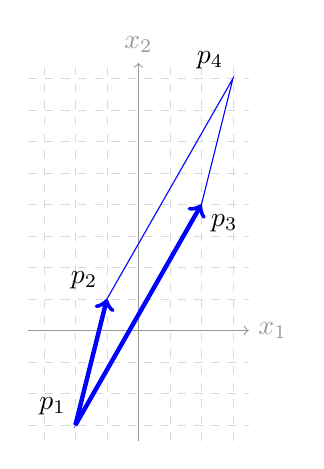
\begin{tikzpicture}[scale=0.4]
\def\XMAX{3.5};\def\YMAX{8.5};
\draw[help lines, color=gray!30, dashed] (-\XMAX,-\YMAX+5) grid (\XMAX,\YMAX);
\draw[->, color=gray!80] (-\XMAX,0)--(\XMAX,0) node[right]{$x_1$};
\draw[->, color=gray!80] (0,-\YMAX+5)--(0,\YMAX) node[above]{$x_2$};
\coordinate (p1) at (-2,-3); \node at (p1)[above left]{$p_1$};
\coordinate (p2) at (-1,1); \node at (p2)[above left]{$p_2$};
\coordinate (p3) at (2,4); \node at (p3)[below right]{$p_3$};
\coordinate (p4) at (3,8); \node at (p4)[above left]{$p_4$};
\draw[blue] (p1)--(p2)--(p4)--(p3)--cycle;
\draw[->,ultra thick,blue] (p1)--(p2);
\draw[->,ultra thick,blue] (p1)--(p3);
\end{tikzpicture}
\end{center}
\end{solution}

\begin{problem}
$\det(A-B)=\det A-\det B$
\end{problem}

\begin{solution}
This is false, for example, we could just take $A=I=\begin{bmatrix}
1&0\\0&1
\end{bmatrix}$, $B=-I$, then $4=\det(2I)=\det(A-B)\neq \det A-\det B=1-1=0$
\end{solution}

\begin{problem}
If $A$ is a 3 by 3 matrix, then $\det(2A)=8(\det A)$
\end{problem}

\begin{solution}
This is true.
\end{solution}

\begin{problem}
Suppose $A,B$ are both 3 by 3 matrices, and $\det A=2$, $\det B=\frac{1}{3}$, then the determinant of $A^TB^{-1}$ is
\end{problem}

\begin{solution}
$\det(A^TB^{-1})=\det(A^T)\det(B^{-1})=(\det A)(\det B)^{-1}=2\cdot 3=6$.
\end{solution}

\begin{problem}
Suppose $A$ is a 3 by 3 matrix with entries integers, and $A^3=I$ is the identity matrix. Then the determinant of $A$ has to be
\end{problem}

\begin{solution}
$\det A$ must be some real number. $1=\det I=\det(A^3)=(\det A)^3\Rightarrow \det A=\sqrt[3]{1}=1$.
\end{solution}

\subsection{Online Assignment 6}

\begin{problem}
Suppose $A=\begin{bmatrix}
1&2&1&2&-1&3\\
0&0&0&0&1&-1\\
0&0&1&3&1&-2\\
\end{bmatrix}$
\begin{enumerate}[label=\alph*)]
\item Find a basis for the null space of $A$
\item Find a basis for the column space of $A$
\item Find a basis for the row space of $A$
\end{enumerate}
\end{problem}

\begin{solution}
First realize
\[
A\xsim{R2\leftrightarrow R3}\begin{bmatrix}
1&2&1&2&-1&3\\
0&0&1&3&1&-2\\
0&0&0&0&1&-1\\
\end{bmatrix}\sim\begin{bmatrix}
1&2&0&-1&0&3\\
0&0&1&3&0&-1\\
0&0&0&0&1&-1\\
\end{bmatrix}
\]
Hence the solution in parametric form is $x_2\begin{bmatrix}
-2\\1\\0\\0\\0\\0
\end{bmatrix}+x_4\begin{bmatrix}
1\\0\\-3\\1\\0\\0
\end{bmatrix}+x_6\begin{bmatrix}
-3\\0\\1\\0\\1\\1
\end{bmatrix}$. And the pivot columns are the 1st, 3rd and 5th columns
\begin{enumerate}[label=\alph*)]
\item A basis for $\Nul A$ could be $\left\{\begin{bmatrix}
-2\\1\\0\\0\\0\\0
\end{bmatrix},\begin{bmatrix}
1\\0\\-3\\1\\0\\0
\end{bmatrix},\begin{bmatrix}
-3\\0\\1\\0\\1\\1
\end{bmatrix}\right\}$
\item A basis for $\Col A$ could be $\left\{\begin{bmatrix}
1\\0\\0
\end{bmatrix},\begin{bmatrix}
1\\0\\1
\end{bmatrix},\begin{bmatrix}
-1\\1\\1
\end{bmatrix}\right\}$
\item A basis for $\Row A$ could be
\[
\left\{\begin{bmatrix}
1&2&0&-1&0&3
\end{bmatrix},\begin{bmatrix}
0&0&1&3&0&-1
\end{bmatrix},\begin{bmatrix}
0&0&0&0&1&-1
\end{bmatrix}\right\}
\]
\end{enumerate}
\end{solution}

\begin{problem}
Suppose $A=\begin{bmatrix}
3&-1&-5\\
1&1&-1\\
-2&2&4\\
\end{bmatrix}$
\begin{enumerate}[label=\alph*)]
\item Determine whether $\mathbf u=\begin{bmatrix}
-3\\1\\-2
\end{bmatrix}$ is in the null space of $A$. Explain your reasoning.
\item Determine whether $\mathbf b=\begin{bmatrix}
1\\-3\\-4
\end{bmatrix}$ is in the column space of $A$. Explain your reasoning.
\end{enumerate}
\end{problem}

\begin{solution}
\begin{enumerate}[label=\alph*)]
\item $\mathbf u\in\Nul A$ since $A\mathbf u=\mathbf0$
\item $\mathbf b\in\Col A$ since linear system $A\mathbf x=\mathbf b$ is consistent
\end{enumerate}
\end{solution}

\begin{problem}
Recall $\mathbb P_2=\{a_0+a_1t+a_2t^2|a_0,a_1,a_2\in\mathbb R\}$ is the set of polynomials of degree less or equal to 2. Let $V$ be the subset of $\mathbb P_2$ consists of polynomials that evalute to 0 at $t=1$ (i.e. polynomial $p(t)$ is in $V$ if $p(1)=0$ and of degree less or equal to 2). With the usual addition and scalar multiplication for polynomials
\begin{enumerate}[label=\alph*)]
\item Show that $V$ is a subspace.
\item Find a basis of $V$.
\item Cosider $T:V\to\mathbb R^2$ that maps polynomial $p(t)$ to $\begin{bmatrix}
p(-1)\\p(2)
\end{bmatrix}$, show $T$ is a linear transformation
\end{enumerate}
\end{problem}

\begin{solution}
\begin{enumerate}[label=\alph*)]
\item Realize that $V=\ker S$ for the linear transformation $S:\mathbb P_2\to\mathbb R$, $S(a_0+a_1t+a_2t^2)=a_0+a_1+a_2$, thus $V$ is a subspace of $\mathbb P_2$
\item This is precisely Example~\ref{10:24-07/01/2022}
\item For any $p(t),q(t)\in V$ and $c\in\mathbb R$, we have
\[
T(p+q)=\begin{bmatrix}
(p+q)(-1)\\(p+q)(2)
\end{bmatrix}=\begin{bmatrix}
p(-1)+q(-1)\\p(2)+q(2)
\end{bmatrix}=\begin{bmatrix}
p(-1)\\p(2)
\end{bmatrix}+\begin{bmatrix}
q(-1)\\q(2)
\end{bmatrix}=T(p)+T(q)
\]
\[
T(cp)=\begin{bmatrix}
(cp)(-1)\\(cp)(2)
\end{bmatrix}=\begin{bmatrix}
c\cdot p(-1)\\c\cdot p(2)
\end{bmatrix}=c\begin{bmatrix}
p(-1)\\p(2)
\end{bmatrix}=cT(p)
\]
Therefore $T:V\to\mathbb R^2$ is a linear transformation
\end{enumerate}
\end{solution}

\begin{problem}
We say a square matrix $A$ is \textcolor{blue}{anti-symmetric}\index{anti-symmetric} if $A^T=-A$. Denote the set of $3\times3$ anti-symmetric matrices $V$.
\begin{enumerate}[label=\alph*)]
\item Show that $V$ is a vector space.
\item What is the dimension of $V$?
\item Find a basis of $V$.
\item Show that
\[
\mathcal B=\left\{B_1=\begin{bmatrix}
0&-1&-1\\
1&0&-1\\
1&1&0\\
\end{bmatrix},B_2=\begin{bmatrix}
0&2&0\\
-2&0&-1\\
0&1&0\\
\end{bmatrix},B_3=\begin{bmatrix}
0&-1&-2\\
1&0&-3\\
2&3&0\\
\end{bmatrix}\right\}
\]
form a basis for $V$.
\end{enumerate}
\end{problem}

\begin{solution}
\begin{enumerate}[label=\alph*)]
\item For any $A,B\in V$ and $c\in\mathbb R$, by definition $A^T=-A, B^T=-B$, so
\[
(A+B)^T=A^T+B^T=-A-B=-(A+B)
\]
\[
(cA)^T=cA^T=c(-A)=-(cA)
\]
hence $A+B,cA\in V$, i.e. $V$ is a closed under addition and scalar multiplication. Therefore $V$ is a subspace of $M_{3\times2}(\mathbb R)$, and consequently a vector space.
\item It is not hard to realize
\[
V=\left\{\begin{bmatrix}
0&-a&-b\\
a&0&-c\\
b&c&0
\end{bmatrix}\in\ M_{3\times3}(\mathbb R)\middle|a,b,c\in\mathbb R\right\}\cong\mathbb R^3
\]
Thus $\dim V=3$
\item Note that
\begin{equation}\label{14:56-06/24/2022}
\begin{aligned}
\begin{bmatrix}
0&-a&-b\\
a&0&-c\\
b&c&0
\end{bmatrix}&=\begin{bmatrix}
0&-a&0\\
a&0&0\\
0&0&0
\end{bmatrix}+\begin{bmatrix}
0&0&-b\\
0&0&0\\
b&0&0
\end{bmatrix}+\begin{bmatrix}
0&0&0\\
0&0&-c\\
0&c&0
\end{bmatrix}\\
&=a\begin{bmatrix}
0&-1&0\\
1&0&0\\
0&0&0
\end{bmatrix}+b\begin{bmatrix}
0&0&-1\\
0&0&0\\
1&0&0
\end{bmatrix}+c\begin{bmatrix}
0&0&0\\
0&0&-1\\
0&1&0
\end{bmatrix}
\end{aligned}
\end{equation}
So we know that
\[
\mathcal E=\{E_1,E_2,E_3\}=
\left\{
\begin{bmatrix}
0&-1&0\\
1&0&0\\
0&0&0
\end{bmatrix},\begin{bmatrix}
0&0&-1\\
0&0&0\\
1&0&0
\end{bmatrix},\begin{bmatrix}
0&0&0\\
0&0&-1\\
0&1&0
\end{bmatrix}\right\}
\]
is a basis for $V$, this is linearly independent since the linear combination \eqref{14:56-06/24/2022} is equal to zero $\iff a=b=c=0$
\item Check that the coordinate vectors $\{[B_1]_{\mathcal E},[B_2]_{\mathcal E},[B_3]_{\mathcal E}\}=\left\{\begin{bmatrix}
1\\1\\1
\end{bmatrix},\begin{bmatrix}
-2\\0\\1
\end{bmatrix},\begin{bmatrix}
1\\2\\3
\end{bmatrix}\right\}$ form a basis for $\mathbb R^3$, so $\mathcal B$ form a basis for $V$.
\end{enumerate}
\end{solution}

\subsection{Online Assignment 7}

\begin{problem}
Suppose $\mathbf v$ is an eigenvector for matrices $A$ and $B$, then $\mathbf v$ is an eigenvector for $A+B$ and $AB$.
\end{problem}

\begin{solution}
This is true. Since $\mathbf v$ is an eigenvector for both $A$ and $B$, there exist eigenvalues $\lambda_1,\lambda_2$ such that $A\mathbf v=\lambda_1\mathbf v$, $B\mathbf v=\lambda_2\mathbf v$, so we have $(A+B)\mathbf v=A\mathbf v+B\mathbf v=\lambda_1\mathbf v+\lambda_2\mathbf v=(\lambda_1+\lambda_2)\mathbf v$. In other words, $\mathbf v$ is an eigenvector for $A+B$ with eigenvalue $\lambda_1+\lambda_2$. Similarly, we also have $AB\mathbf v=A(\lambda_1\mathbf v_1)=\lambda_2 A\mathbf v=\lambda_1\lambda_2\mathbf v$. In other words, $\mathbf v$ is an eigenvector for $AB$ with eigenvector $\lambda_1\lambda_2$
\end{solution}

\begin{problem}
Suppose $t+3t^2-2t^3$ is the characteristic polynomial of a 3 by 3 matrix, then $A$ is not invertible.
\end{problem}

\begin{solution}
This is true. Note that $t=0$ is a root of the characteristic polynomial, so the null space of $A$ is not trivial, $A$ is not invertible.
\end{solution}

\begin{problem}
Suppose $\mathcal B=\left\{1+t,1+2t^2,1-t+t^2\right\}$ and $\mathcal C=\left\{1-t,t,t^2\right\}$ are two bases for $\mathbb P_2$, What is the change of basis matrix $\underset{\mathcal C\leftarrow\mathcal B}{P}$ from $\mathcal B$ to $\mathcal C$. Please show all your work.
\end{problem}

\begin{solution}
First let's find the change of basis matrices from $\mathcal B$ and $\mathcal C$ to the standard basis $\mathcal E=\{1,t,t^2\}$. We have
\[
\underset{\mathcal E\leftarrow\mathcal B}{P}=\begin{bmatrix}
[1+t]_{\mathcal E}&[1+2t^2]_{\mathcal E}&[1-t+t^2]_{\mathcal E}
\end{bmatrix}=\begin{bmatrix}
1&1&1\\
1&0&-1\\
0&2&1
\end{bmatrix}
\]
And
\[
\underset{\mathcal E\leftarrow\mathcal C}{P}=\begin{bmatrix}
[1-t]_{\mathcal E}&[t]_{\mathcal E}&[t^2]_{\mathcal E}
\end{bmatrix}=\begin{bmatrix}
1&0&0\\
-1&1&0\\
0&0&1
\end{bmatrix}
\]
Hence we have
\begin{align*}
\underset{\mathcal C\leftarrow\mathcal B}{P}=\left(\underset{\mathcal C\leftarrow\mathcal E}{P}\right)\left(\underset{\mathcal E\leftarrow\mathcal B}{P}\right)=\left(\underset{\mathcal E\leftarrow\mathcal C}{P}\right)^{-1}\left(\underset{\mathcal E\leftarrow\mathcal B}{P}\right)=\begin{bmatrix}
1&0&0\\
-1&1&0\\
0&0&1
\end{bmatrix}^{-1}\begin{bmatrix}
1&1&1\\
1&0&-1\\
0&2&1
\end{bmatrix}=\begin{bmatrix}
1       &       1  &            1       \\
2        &      1 &             0       \\
0         &     2&              1 
\end{bmatrix}
\end{align*}
\end{solution}

\begin{problem}
If $Nul A$ is 2-dimensional, then $0$ is an eigenvalue of $A$.
\end{problem}

\begin{solution}
This is true. Since if $\Nul A$ is 2-dimensional, then $\Nul A$ is non-trivial, thus $0$ is an eigenvalue of $A$
\end{solution}

\begin{problem}
Is $\begin{bmatrix}0\\0\\1\end{bmatrix}$ an eigenvector of $\begin{bmatrix}2&0&0\\3&2&0\\0&4&3\end{bmatrix}$? If so, find the corresponding eigenvalue, if not, please explain why.
\end{problem}

\begin{solution}
Note that $\begin{bmatrix}2&0&0\\3&2&0\\0&4&3\end{bmatrix}\begin{bmatrix}0\\0\\1\end{bmatrix}=\begin{bmatrix}0\\0\\3\end{bmatrix}$. so $\begin{bmatrix}0\\0\\1\end{bmatrix}$ is an eigenvector with eigenvalue 3
\end{solution}

\begin{problem}
Find all eigenvalues of $A=\begin{bmatrix}6&-2&0\\-2&9&0\\5&8&3\end{bmatrix}$. Please show all your work.
\end{problem}

\begin{solution}
\begin{align*}
\left|tI-A\right|&=\left|\begin{matrix}
t-6&2&0\\
2&t-9&0\\
-5&-8&t-3
\end{matrix}\right|\xequal{\text{cofator expansion across 3rd column}}(t-3)(-1)^{3+3}\left|\begin{matrix}
t-6&2\\
2&t-9
\end{matrix}\right|\\
&=(t-3)((t-6)(t-9)-2\cdot 2)=(t-3)(t^2-5t+50)=(t-3)(t-5)(t-10)
\end{align*}
Therefore eigenvalues for $A$ are 3,5,10.
\end{solution}

\begin{problem}
Assume that $A$ is similar to an upper triangular matrix $U$, then $\det A$ is the product of all its eigenvalues (counting multiplicity). Please explain why.
\end{problem}

\begin{solution}
Suppose the diagonal elements of $A$ are $\lambda_1,\cdots,\lambda_n$, then the charateristic polynomial of $A$ is the same the charateristic polynomial $U$ (Since they are similar) which would be $(t-\lambda_1)\cdots(t-\lambda_n)$, so $\lambda_1,\cdots,\lambda_n$ are the eigenvalues for $A$. And the determinant of $A$ is the same as the determinant of $U$ (Since they are similar) which is $\lambda_1\cdots\lambda_n$
\end{solution}

\subsection{Online Assignment 8}

\begin{problem}
Suppose $A=\begin{bmatrix}
2&2&1\\
1&3&1\\
1&2&2
\end{bmatrix}$, determine whether $A$ is diagonalizable. If it is, please find a diagonalization. If not, please explain why.
\end{problem}

\begin{solution}
First we evaluate the characteristic polynomial of $A$
\begin{align*}
\det(tI-A)&=\left|\begin{matrix}
t-2&-2&-1\\
-1&t-3&-1\\
-1&-2&t-2
\end{matrix}\right|\xequal{\substack{R1\rightarrow R1+(t-2)R3\\R2\rightarrow R2-R3}}\left|\begin{matrix}
0&-2(t-1)&(t-1)(t-3)\\
0&t-1&-(t-1)\\
-1&-2&t-2
\end{matrix}\right|\\
&\xequal{\text{factor out $(t-1)$ on row 1 and row 2}}(t-1)^2\left|\begin{matrix}
0&-2&(t-3)\\
0&1&-1\\
-1&-2&t-2
\end{matrix}\right|=(t-1)^2(t-5)
\end{align*}
So the eigenvalues are $\lambda_1=\lambda_2=1$, $\lambda_3=5$. For the 1-eigenspace, we consider
\begin{align*}
\left[\begin{array}{c|c}
I-A&\mathbf0
\end{array}\right]&=
\left[\begin{array}{ccc|c}
-1&-2&-1&0\\
-1&-2&-1&0\\
-1&-2&-1&0
\end{array}\right]\sim\left[\begin{array}{ccc|c}
1&2&1&0\\
0&0&0&0\\
0&0&0&0
\end{array}\right]
\end{align*}
So we get two basis vectors $\left\{\mathbf v_1=\begin{bmatrix}
-2\\1\\0
\end{bmatrix},\mathbf v_2=\begin{bmatrix}
-1\\0\\1
\end{bmatrix}\right\}$. For the 5-eigenspace, we consider
\begin{align*}
\left[\begin{array}{c|c}
5I-A&\mathbf0
\end{array}\right]&=
\left[\begin{array}{ccc|c}
3&-2&-1&0\\
-1&2&-1&0\\
-1&-2&3&0
\end{array}\right]\sim\left[\begin{array}{ccc|c}
1&0&-1&0\\
0&1&-1&0\\
0&0&0&0
\end{array}\right]
\end{align*}
So we get a basis vector $\left\{\mathbf v_3=\begin{bmatrix}
1\\1\\1
\end{bmatrix}\right\}$
\item From above, we get the diagonalization
\[
A=PDP^{-1}=\begin{bmatrix}
-2&-1&1\\
1&0&1\\
0&1&1
\end{bmatrix}\begin{bmatrix}
1&0&0\\
0&1&0\\
0&0&5
\end{bmatrix}\begin{bmatrix}
-\frac{1}{4}&\frac{1}{2}&-\frac{1}{4}\\
-\frac{1}{4}&-\frac{1}{2}&\frac{3}{4}\\
\frac{1}{4}&\frac{1}{2}&\frac{1}{4}
\end{bmatrix}
\]
\end{solution}

\begin{problem}
Suppose $A=\begin{bmatrix}
-6&8\\
-4&6
\end{bmatrix}$, Please evaluate $A^{101}$, show all your work.
\end{problem}

\begin{solution}
First we can diagonalize $A$ as
\[
A=\begin{bmatrix}
1&2\\
1&1
\end{bmatrix}\begin{bmatrix}
2&0\\
0&-2
\end{bmatrix}\begin{bmatrix}
-1&2\\
1&-1
\end{bmatrix}
\]
\[
A^{101}=PD^{101}P^{-1}=\begin{bmatrix}
1&2\\
1&1
\end{bmatrix}\begin{bmatrix}
2^{101}&0\\
0&-2^{101}
\end{bmatrix}\begin{bmatrix}
-1&2\\
1&-1
\end{bmatrix}
\]
\end{solution}

\begin{problem}
Suppose $T:\mathbb R^3\to\mathbb R^3$ is a linear transformation, $\mathcal B=\{\mathbf b_1,\mathbf b_2,\mathbf b_3\}$, $\mathcal C=\{\mathbf c_1,\mathbf c_2,\mathbf c_3\}$ are two different bases for $\mathbb R^3$. Determine whether the following is possible.
\begin{enumerate}[label=\alph*)]
\item $[T]_{\mathcal B}=\begin{bmatrix}
1 &2&4\\
3 &-1 &-2\\
2 &-1& 3
\end{bmatrix}$ and $[T]_{\mathcal C}=\begin{bmatrix}
1& -3 &1\\
2 &1& 6\\
0 &3 &8
\end{bmatrix}$
\item $[T]_{\mathcal B}=\begin{bmatrix}
3&0&0\\
2&2&0\\
2&3&4
\end{bmatrix}$ and $[T]_{\mathcal C}=\begin{bmatrix}
1&-1&0\\
2&4&0\\
3&-2&4
\end{bmatrix}$
\end{enumerate}
\end{problem}

\begin{solution}
\begin{enumerate}[label=\alph*)]
\item This is not possible since these two matrices have different determinant.
\item This is possible since these two matrix has the same the characteristic polynomial $(t-2)(t-3)(t-4)$, hence they are similar to same diagonal matrix, and thus similar.
\end{enumerate}
\end{solution}

\begin{problem}
Suppose $A$ is similar to $B$.
\begin{enumerate}[label=\alph*)]
\item Could you conclude that $3A$ is similar to $3B$. If you can, please give your reasons, if not, please find a counter-example.
\item Could you conclude that $A^{-1}$ is similar to $B^{-1}$. If you can, please give your reasons, if not, please find a counter-example.
\end{enumerate}
\end{problem}

\begin{solution}
Since $A$ is similar to $B$, we may assume $A=PBP^{-1}$.
\begin{enumerate}[label=\alph*)]
\item $3A=3PBP^{-1}=P(3B)P^{-1}$ is similar.
\item $A^{-1}=(PBP^{-1})^{-1}=PB^{-1}P^{-1}$ is similar.
\end{enumerate}
\end{solution}

\subsection{Online Assignment 9}

\begin{problem}
Determine whether the following statements are true
\begin{enumerate}[label=\alph*)]
\item $\|\mathbf u\|^2+\|\mathbf v\|^2=\|\mathbf u+\mathbf v\|^2$ if and only if $\mathbf u,\mathbf v$ are orthogonal.
\item If $W$ is a subspace of $\mathbb R^n$, and vector $\mathbf v$ is orthogonal to both $W$ and $W^\perp$, then $\mathbf v=\mathbf0$.
\item If $W = \Span\{\mathbf x_1, \mathbf x_2 ,\mathbf x_3\}$ with $\{\mathbf x_1, \mathbf x_2 ,\mathbf x_3\}$ linearly independent, and if $\{\mathbf v_1, \mathbf v_2 ,\mathbf v_3\}$ is an orthogonal set in $W$, then $\{\mathbf v_1, \mathbf v_2 ,\mathbf v_3\}$ is a basis for $W$.
\end{enumerate}
\end{problem}

\begin{solution}
\begin{enumerate}[label=\alph*)]
\item This is true. $\|\mathbf u+\mathbf v\|^2=(\mathbf u+\mathbf v)\cdot(\mathbf u+\mathbf v)=\mathbf u\cdot\mathbf u+2\mathbf u\cdot\mathbf v+\mathbf v\cdot\mathbf v=\|\mathbf u\|^2+\|\mathbf v\|^2+2\mathbf u\cdot\mathbf v$. Thus the equality holds $\iff\mathbf u\cdot\mathbf v=0$, i.e. $\mathbf u,\mathbf v$ are orthogonal.
\item Consider $\mathbf v\cdot\mathbf v=\|\mathbf v\|^2$, it should be 0 since $\mathbf v$ is in both $W$ and $W^\perp$, so $\mathbf v=\mathbf 0$
\item This is true by Theorem~\ref{01:12-07/15/2022}
\end{enumerate}
\end{solution}

\begin{problem}
Suppose $A=\begin{bmatrix}
1&2&3\\
2&1&-1\\
0&2&4\\
3&5&-1
\end{bmatrix}$, please find a basis for $(\Col A)^\perp$.
\end{problem}

\begin{solution}
Recall that $(\Col A)^\perp=\Nul(A^T)$. And we can find a basis for $\Nul(A^T)$ through
\[
\left[\begin{array}{c|c}
A^T&\mathbf0
\end{array}\right]=\left[\begin{array}{cccc|c}
1&2&0&3&0\\
2&1&2&5&0\\
3&-1&4&1&0
\end{array}\right]\sim\left[\begin{array}{cccc|c}
1&0&0&-13&0\\
0&1&0&8&0\\
0&0&1&\frac{23}{2}&0
\end{array}\right]
\]
Thus
\[
(\Col A)^\perp=\Span\left\{\begin{bmatrix}
13\\-8\\-\frac{23}{2}\\1
\end{bmatrix}\right\}
\]
\end{solution}

\begin{problem}
Suppose we have $\mathcal B=\left\{\mathbf u_1=\begin{bmatrix}1\\1\\0\\-1\end{bmatrix},\mathbf u_2=\begin{bmatrix}1\\0\\1\\1\end{bmatrix},\mathbf u_3=\begin{bmatrix}0\\-1\\1\\-1\end{bmatrix}\right\}$, please justify that $\mathcal B$ is an orthogonal set, suppose $\mathbf y=\begin{bmatrix}1\\2\\3\\4\end{bmatrix}$, $L$ is the subspace spanned by $\mathcal B$, compute the projection $\Proj_L\mathbf y$ of $\mathbf y$ onto $L$.
\end{problem}

\begin{solution}
Let $A=\begin{bmatrix}
\mathbf u_1&\mathbf u_2&\mathbf u_3
\end{bmatrix}=\begin{bmatrix}
1&1&0\\
1&0&-1\\
0&1&1\\
-1&1&-1
\end{bmatrix}$, we can check that $A^TA=I$ is the 3 by 3 identity matrix, so $\mathcal B$ is an orthogonal set. And therefore
\begin{align*}
\Proj_L\mathbf y&=\frac{\mathbf y\cdot\mathbf u_1}{\mathbf u_1\cdot\mathbf u_1}\mathbf u_1+\frac{\mathbf y\cdot\mathbf u_2}{\mathbf u_2\cdot\mathbf u_2}\mathbf u_2+\frac{\mathbf y\cdot\mathbf u_3}{\mathbf u_3\cdot\mathbf u_3}\mathbf u_3\\
&=\frac{-1}{3}\mathbf u_1+\frac{8}{3}\mathbf u_2+\frac{-3}{3}\mathbf u_3\\
&=-\frac{1}{3}\begin{bmatrix}
1\\1\\0\\-1
\end{bmatrix}+\frac{8}{3}\begin{bmatrix}
1\\0\\1\\1
\end{bmatrix}-\begin{bmatrix}
0\\-1\\1\\-1
\end{bmatrix}=\begin{bmatrix}
\frac{7}{3}\\\frac{2}{3}\\\frac{5}{3}\\4
\end{bmatrix}
\end{align*}
\end{solution}

\begin{problem}
Suppose $A=\begin{bmatrix}
-1&6&6\\
3&-8&3\\
1&-2&6\\
1&-4&-3
\end{bmatrix}$, please find an orthogonal basis for $\Col A$.
\end{problem}

\begin{solution}
We apply the Gram-Schmidt process here
\begin{itemize}
\item $\mathbf u_1=\mathbf v_1=\begin{bmatrix}
-1\\3\\1\\1
\end{bmatrix}$
\item $\mathbf u_2=\mathbf v_2-\dfrac{\mathbf v_2\cdot\mathbf u_1}{\mathbf u_1\cdot\mathbf u_1}\mathbf u_1=\begin{bmatrix}
6\\-8\\-2\\-4
\end{bmatrix}-\frac{-36}{12}\begin{bmatrix}
-1\\3\\1\\1
\end{bmatrix}=\begin{bmatrix}
3\\1\\1\\-1
\end{bmatrix}$
\item $\mathbf u_3=\mathbf v_3-\dfrac{\mathbf v_3\cdot\mathbf u_1}{\mathbf u_1\cdot\mathbf u_1}\mathbf u_1-\dfrac{\mathbf v_3\cdot\mathbf u_2}{\mathbf u_2\cdot\mathbf u_2}\mathbf u_2=\begin{bmatrix}
6\\3\\6\\-3
\end{bmatrix}-\frac{6}{12}\begin{bmatrix}
-1\\3\\1\\1
\end{bmatrix}-\frac{30}{12}\begin{bmatrix}
3\\1\\1\\-1
\end{bmatrix}=\begin{bmatrix}
-1\\-1\\3\\-1
\end{bmatrix}$
\end{itemize}
So we have an orthogonal basis for $\Col A$
\[
\Col A=\Span\left\{\begin{bmatrix}
-1\\3\\1\\1
\end{bmatrix},\begin{bmatrix}
3\\1\\1\\-1
\end{bmatrix},\begin{bmatrix}
-1\\-1\\3\\-1
\end{bmatrix}\right\}
\]
\end{solution}

\subsection{Online Assignment 10}

\begin{problem}
Determine whether the following statements are correct
\begin{enumerate}[label=\alph*)]
\item If $A$ is symmetric and if vectors $\mathbf u$ and $\mathbf v$ such that $A\mathbf u = \mathbf u$ and $\mathbf v$ is in $\operatorname{Nul}A$, then $\mathbf u \cdot\mathbf v = \mathbf0$.
\item $\operatorname{Nul}A=\operatorname{Nul}A^TA$.
\end{enumerate}
\end{problem}

\begin{solution}
\begin{enumerate}[label=\alph*)]
\item The eigenvalues for eigenvectors $\mathbf u$ and $\mathbf v$ are 1 and 0, and $A$ is symmetric, by Theorem~\ref{23:54-07/19/2022}, $\mathbf u\cdot\mathbf v=0$.
\item If $\mathbf x\in\Nul A$, then $A\mathbf x=\mathbf0$, so $A^TA\mathbf x=\mathbf 0$. If $\mathbf x\in\Nul(A^TA)$, then $A^TA\mathbf x=\mathbf0$, so $0=\mathbf x^TA^TA\mathbf x=\|A\mathbf x\|^2$, so $A\mathbf x=0$.
\end{enumerate}
\end{solution}

\begin{problem}
Find the least-squares solution(s) to $\begin{bmatrix}
1&5\\
3&1\\
-2&4
\end{bmatrix}\begin{bmatrix}
x_1\\x_2
\end{bmatrix}=\begin{bmatrix}
4\\-2\\-3
\end{bmatrix}$.
\end{problem}

\begin{solution}
Let's denote $A=\begin{bmatrix}
1&5\\
3&1\\
-2&
\end{bmatrix}$, $\mathbf b=\begin{bmatrix}
4\\-2\\-3
\end{bmatrix}$, then $A^TA=\begin{bmatrix}
14&0\\
0&42
\end{bmatrix}$, and $A^T\mathbf b=\begin{bmatrix}
4\\6
\end{bmatrix}$, then we get the least -square solution $\hat{\mathbf x}=(A^TA)^{-1}A^T\mathbf b=\begin{bmatrix}
\frac{2}{7}\\\frac{1}{7}
\end{bmatrix}$
\end{solution}

\begin{problem}
Orthogonal diagonalize the matrix $\begin{bmatrix}
3&4\\
4&9
\end{bmatrix}$.
\end{problem}

\begin{solution}
First note that $A=\begin{bmatrix}
3&4\\
4&9
\end{bmatrix}$ is symmetric and real-valued, we can get its eigenvalues $\lambda_1=1$, $\lambda_2=11$, and normalized eigenvectors $\mathbf u_1=\begin{bmatrix}
-\frac{2}{\sqrt5}\\\frac{1}{\sqrt5}
\end{bmatrix}$, $\mathbf u_2=\begin{bmatrix}
\frac{1}{\sqrt5}\\\frac{2}{\sqrt5}
\end{bmatrix}$. Hence we have the orthogonal diganolization
\[
A=\begin{bmatrix}
3&4\\
4&9
\end{bmatrix}=\begin{bmatrix}
-\frac{2}{\sqrt5}&\frac{1}{\sqrt5}\\
\frac{1}{\sqrt5}&\frac{2}{\sqrt5}
\end{bmatrix}\begin{bmatrix}
1&0\\0&11
\end{bmatrix}\begin{bmatrix}
-\frac{2}{\sqrt5}&\frac{1}{\sqrt5}\\
\frac{1}{\sqrt5}&\frac{2}{\sqrt5}
\end{bmatrix}=PDP^T
\]
\end{solution}

\begin{problem}
Suppose $A=\begin{bmatrix}
1&5\\
-2&3
\end{bmatrix}$.
\begin{enumerate}[label=\alph*)]
\item Please find the eigenvalues of $A$.
\item Please find the eigenvectors of $A$.
\item Please write $A$ as matrix multiplication $PCP^{-1}$, where $C$ is of the form $\begin{bmatrix}
a&-b\\
b&c
\end{bmatrix}$.
\end{enumerate}
\end{problem}

\begin{solution}
\begin{enumerate}[label=\alph*)]
\item The characteristic polynomial is $t^2-4t+13$, and so the eigenvalues are $\lambda=2-3i$, $\overline\lambda=2+3i$, so we have $a=2$, $b=3$ and $C=\begin{bmatrix}
2&-3\\3&2
\end{bmatrix}$
\item The eigenvalues for $\lambda,\overline{\lambda}$ are $\mathbf v=\begin{bmatrix}
1+3i\\2
\end{bmatrix}=\begin{bmatrix}
1\\2
\end{bmatrix}+i\begin{bmatrix}
3\\0
\end{bmatrix}$, $\overline{\mathbf v}=\begin{bmatrix}
1-3i\\2
\end{bmatrix}$. so $P=\begin{bmatrix}
1&3\\
2&0
\end{bmatrix}$
\item From above computation we get decomposition
\[
A=\begin{bmatrix}
1&3\\
2&0
\end{bmatrix}\begin{bmatrix}
2&-3\\3&2
\end{bmatrix}\begin{bmatrix}
0&\frac{1}{2}\\
\frac{1}{3}&-\frac{1}{6}
\end{bmatrix}=PCP^{-1}
\]
\end{enumerate}
\end{solution}

\section{Exams}

\subsection{Exam 1}

\begin{problem}\hfill
\begin{enumerate}[label=\textbf{\alph*)}]
\item\textbf{(15 pt)} Write linear system
\[
\systeme{2x_1+4x_2+2x_3=2, x_1+3x_2-x_3+2x_4=1, -x_1+2x_2+3x_3+2x_4=-1}
\]
as a matrix equation, and then solve it, write your solution in parametric vector form.
\item\textbf{(5 pt)} Is $\left\{\mathbf a_1=\begin{bmatrix}
2\\1\\-1
\end{bmatrix},\mathbf a_2=\begin{bmatrix}
4\\3\\2
\end{bmatrix},\mathbf a_3=\begin{bmatrix}
2\\-1\\3
\end{bmatrix},\mathbf a_4=\begin{bmatrix}
0\\2\\2
\end{bmatrix}\right\}$ linearly independent? Why or why not.
\item\textbf{(4 pt)} What is the span of $\{\mathbf a_1,\mathbf a_2,\mathbf a_3,\mathbf a_4\}$
\end{enumerate}
\end{problem}

\begin{solution}
\begin{enumerate}[label=\textbf{\alph*)}]
\item We could rewrite the linear system as
\[
A\mathbf x=\begin{bmatrix}
2&4&2&0\\
1&3&-1&2\\
-1&2&3&2
\end{bmatrix}\begin{bmatrix}
x_1\\x_2\\x_3\\x_4
\end{bmatrix}=\begin{bmatrix}
2\\1\\-1
\end{bmatrix}=\mathbf b
\]
\begin{align*}
&\begin{bmatrix}
A&\mathbf b
\end{bmatrix}\xsim{\substack{R3\rightarrow R3+R2\\R1\rightarrow R1-2R2}}\begin{bmatrix}
0&-2&4&-4&0\\
1&3&-1&2&1\\
0&5&2&4&0
\end{bmatrix}\xsim{R1\leftrightarrow R2}\begin{bmatrix}
1&3&-1&2&1\\
0&-2&4&-4&0\\
0&5&2&4&0
\end{bmatrix}\\
&\xsim{R2\to R2/(-2)}\begin{bmatrix}
1&3&-1&2&1\\
0&1&-2&2&0\\
0&5&2&4&0
\end{bmatrix}\xsim{\substack{R1\rightarrow R1-3R2\\R3\to R3-5R2}}\begin{bmatrix}
1&0&5&-4&1\\
0&1&-2&2&0\\
0&0&12&-6&0
\end{bmatrix}\\
&\xsim{R3\to R3/12}\begin{bmatrix}
1&0&5&-4&1\\
0&1&-2&2&0\\
0&0&1&-\frac{1}{2}&0
\end{bmatrix}\xsim{\substack{R1\rightarrow R1-5R3\\R2\rightarrow R2+2R3}}\begin{bmatrix}
1&0&0&-\frac{3}{2}&1\\
0&1&0&1&0\\
0&0&1&-\frac{1}{2}&0
\end{bmatrix}
\end{align*}
So the solution is
\[
\begin{cases}
x_1=1+\frac{3}{2}x_4\\
x_2=-x_4\\
x_3=\frac{1}{2}x_4\\
x_4\text{ is free}
\end{cases}\Rightarrow\,
\begin{bmatrix}
x_1\\x_2\\x_3\\x_4
\end{bmatrix}=\begin{bmatrix}
1\\0\\0\\0
\end{bmatrix}+x_4\begin{bmatrix}
\frac{3}{2}\\-1\\\frac{1}{2}\\1
\end{bmatrix}
\]
\item Note $A=\begin{bmatrix}
\mathbf a_1&\mathbf a_2&\mathbf a_3&\mathbf a_4
\end{bmatrix}$ has RREF $\begin{bmatrix}
1&0&0&-\frac{3}{2}\\
0&1&0&1\\
0&0&1&-\frac{1}{2}
\end{bmatrix}$. Since the fourth each column is not a pivot column, $\{\mathbf a_1,\mathbf a_2,\mathbf a_3,\mathbf a_4\}$ is linearly dependent.
\item Since the RREF $A$ has a pivot in each row, the columns of $A$ (i.e. $\{\mathbf a_1,\mathbf a_2,\mathbf a_3,\mathbf a_4\}$) span $\mathbb R^3$
\end{enumerate}
\end{solution}

\begin{problem}
Suppose $T:\mathbb R^3\to\mathbb R^3$ is a linear transformation defined by $T\left(\begin{bmatrix}
x_1\\x_2\\x_3
\end{bmatrix}\right)=\begin{bmatrix}
x_1+2x_2+3x_3\\2x_1+5x_3\\2x_1+3x_2+6x_3
\end{bmatrix}$. Denote the standard matrix for $T$ as $A$.
\begin{enumerate}[label=\textbf{\alph*)}]
\item\textbf{(3 pt)} Evaluate $A$.
\item\textbf{(4 pt)} Is $T$ is onto? Is $T$ one-to-one?
\item\textbf{(17 pt)} Is $T$ is invertible? If so, what is the standard matrix for $T^{-1}$?
\item\textbf{(15 pt)} Find $A^T$ ,$(A^T)^{-1}$.
\end{enumerate}
\end{problem}

\begin{solution}
\begin{enumerate}[label=\textbf{\alph*)}]
\item The standard matrix for $T$ is $A=\begin{bmatrix}
1&2&3\\
2&0&5\\
2&3&6
\end{bmatrix}$
\item $T$ is onto and one-to-to.
\item $T$ is invertible. And the standard matrix of $T^{-1}$ is $A^{-1}$
\begin{align*}
&\left[\begin{array}{c|c}
A&I
\end{array}\right]=\left[\begin{array}{ccc|ccc}
1&2&3&1&0&0\\
2&0&5&0&1&0\\
2&3&6&0&0&1
\end{array}\right]\xsim{\substack{R2\rightarrow R2-2R1\\R3\rightarrow R3-2R1}}\left[\begin{array}{ccc|ccc}
1&2&3&1&0&0\\
0&-4&-1&-2&1&0\\
0&-1&0&-2&0&1
\end{array}\right]\\
&\xsim{\substack{R2\rightarrow R2-4R3\\R1\rightarrow R1+2R3}}\left[\begin{array}{ccc|ccc}
1&0&3&-3&0&2\\
0&0&-1&6&1&-4\\
0&-1&0&-2&0&1
\end{array}\right]\xsim{\substack{R2\to(-1)R2\\R3\to(-1)R3}}\left[\begin{array}{ccc|ccc}
1&0&3&-3&0&2\\
0&0&1&-6&-1&4\\
0&1&0&2&0&-1
\end{array}\right]\\
&\xsim{R2\leftrightarrow R3}\left[\begin{array}{ccc|ccc}
1&0&3&-3&0&2\\
0&1&0&2&0&-1\\
0&0&1&-6&-1&4
\end{array}\right]\xsim{R1\rightarrow R1-2R3}\left[\begin{array}{ccc|ccc}
1&0&0&15&3&-10\\
0&1&0&2&0&-1\\
0&0&1&-6&-1&4
\end{array}\right]\\
&=\left[\begin{array}{c|c}
I&A^{-1}
\end{array}\right]
\end{align*}
Hence $A^{-1}=\begin{bmatrix}
15&3&-10\\
2&0&-1\\
-6&-1&4
\end{bmatrix}$
\item $A^T=\begin{bmatrix}
1&2&2\\
2&0&3\\
3&5&6
\end{bmatrix}$, $(A^T)^{-1}=(A^{-1})^T=\begin{bmatrix}
15&2&-6\\
3&0&-1\\
-10&-1&4
\end{bmatrix}$
\end{enumerate}
\end{solution}

\begin{problem}\hfill
\begin{enumerate}[label=\textbf{\alph*)}]
\item\textbf{(5 pt)} Suppose $A=\begin{bmatrix}
1&0&0&0&0&8\\
0&0&h&0&k&-4\\
0&0&0&0&1&0
\end{bmatrix}$ is of reduced row echelon form (RREF), could we know what $h,k$ are? If not, please explain why, if so, please give their values.
\item\textbf{(3 pt)} \texttt{TRUE} or \texttt{FALSE}. If $T:\mathbb R^3\to\mathbb R^3$ is a one-to-one linear transformation, then it is also onto.
\item\textbf{(3 pt)} \texttt{TRUE} or \texttt{FALSE}. If $A$ is a 3 by 3 matrix and $A^5$ is invertible, then so is $A$.
\item\textbf{(3 pt)} \texttt{TRUE} or \texttt{FALSE}. If $A$ is a 5 by 3 matrix, then $A\mathbf x=\mathbf b$ cannot have non-trivial solution(s)
\end{enumerate}
\end{problem}

\begin{solution}
\begin{enumerate}[label=\textbf{\alph*)}]
\item $h=1$, $k=0$. Since $h$ has be in a pivot position, and $k$ is in a pivot column.
\item \texttt{TRUE}. Since its standard matrix would have a pivot in each column, that is three pivots, so there must be a pivot in each row also, hence $T$ is also onto.
\item \texttt{TRUE}. Since $A^5$ is invertible, we may assume its inverse is $B=(A^5)^{-1}$, so that $A^5B=BA^5=I$. Let's show $A^{-1}=A^4B$, first we note that
\[
A^4B=IA^4B=(BA^5)A^4B=BA^9B=BA^4(A^5B)=BA^4I=BA^4
\]
then
\[
AA^{-1}=A(A^4B)=A^5B=I
\]
\[
A^{-1}A=(A^4B)A=(BA^4)A=BA^5=I
\]
Alternatively, we could consider its determinant $0\neq\det(A^5)=(\det A)^5\Rightarrow\det A\neq0$, hence $A$ is invertible.
\item \texttt{FALSE}. Take $A$ to be $\begin{bmatrix}
1&1&1\\
0&0&0\\
0&0&0\\
0&0&0\\
0&0&0\\
\end{bmatrix}$, and $\mathbf b=\mathbf 0$, and the linear system have two free variables.
\end{enumerate}
\end{solution}

\begin{problem}
Suppose $T_1$, $T_2$, $T_3$ and $T$ are all linear transformations from the $xy$-plane to itself.
\begin{enumerate}[label=\textbf{\alph*)}]
\item\textbf{(6 pt)} $T_1$ takes a vector and rotates it \textbf{clockwise} around the origin through an angle $45^\circ$. Writes down its standard matrix $A_1$.
\item\textbf{(6 pt)} $T_2$ reflects over the $x$-axis. Writes down its standard matrix $A_2$.
\item\textbf{(6 pt)} $T_3$ switches $x,y$ coordinates. Writes down its standard matrix $A_3$.
\item\textbf{(6 pt)} Suppose $T$ is such that $T(\mathbf x)=T_3(T_2(T_1(\mathbf x)))$. What the standard matrix of $T$?
\end{enumerate}
\end{problem}

\begin{solution}
\begin{enumerate}[label=\textbf{\alph*)}]
\item The standard matrix $A_1=\begin{bmatrix}
\cos(-45^\circ)&\cos(45^\circ)\\\sin(-45^\circ)&\sin(45^\circ)
\end{bmatrix}=\begin{bmatrix}
\frac{\sqrt2}{\sqrt2}&\frac{\sqrt2}{\sqrt2}\\-\frac{\sqrt2}{\sqrt2}&\frac{\sqrt2}{\sqrt2}
\end{bmatrix}$
\item The standard matrix $A_2=\begin{bmatrix}
1&0\\0&-1
\end{bmatrix}$
\item The standard matrix $A_3=\begin{bmatrix}
0&1\\1&0
\end{bmatrix}$
\item The standard matrix
\begin{align*}
A&=A_3A_2A_1=\begin{bmatrix}
0&1\\1&0
\end{bmatrix}\begin{bmatrix}
1&0\\0&-1
\end{bmatrix}\begin{bmatrix}
\frac{\sqrt2}{\sqrt2}&\frac{\sqrt2}{\sqrt2}\\-\frac{\sqrt2}{\sqrt2}&\frac{\sqrt2}{\sqrt2}
\end{bmatrix}\\
&=\begin{bmatrix}
0&-1\\1&0
\end{bmatrix}\begin{bmatrix}
\frac{\sqrt2}{\sqrt2}&\frac{\sqrt2}{\sqrt2}\\-\frac{\sqrt2}{\sqrt2}&\frac{\sqrt2}{\sqrt2}
\end{bmatrix}\\
&=\begin{bmatrix}
\frac{\sqrt2}{\sqrt2}&-\frac{\sqrt2}{\sqrt2}\\\frac{\sqrt2}{\sqrt2}&\frac{\sqrt2}{\sqrt2}
\end{bmatrix}
\end{align*}
\end{enumerate}
\end{solution}

% \begin{problem}
% Suppose $A=\begin{bmatrix}
% 1&0&3&0\\
% 2&0&6&1\\
% 2&1&2&-4\\
% 3&0&2&1
% \end{bmatrix}$.
% \begin{enumerate}[label=\textbf{\alph*)}]
% \item\textbf{(16 pt)} Evaluate $\det A$.
% \item\textbf{(3 pt)} Is $A$ invertible?
% \item\textbf{(4 pt)} What is $\det(-2A)$?
% \end{enumerate}
% \end{problem}

% \begin{solution}
% \begin{enumerate}[label=\textbf{\alph*)}]
% \item 
% \begin{align*}
% &\left|\begin{matrix}
% 1&0&3&0\\
% 2&0&6&1\\
% 2&1&2&-4\\
% 3&0&2&1
% \end{matrix}\right|\xequal{\text{cofactor expansion across second column}}1(-1)^{3+2}\left|\begin{matrix}
% 1&3&0\\
% 2&6&1\\
% 3&2&1
% \end{matrix}\right|\\
% &\xequal{\substack{R2\rightarrow R2-2R1\\R3\rightarrow R3-3R1}}(-1)\left|\begin{matrix}
% 1&3&0\\
% 0&0&1\\
% 0&-7&1
% \end{matrix}\right|\xequal{R2\leftrightarrow R3}(-1)(-1)\left|\begin{matrix}
% 1&3&0\\
% 0&-7&1\\
% 0&0&1\\
% \end{matrix}\right|=(-1)(-1)1(-7)1=-7
% \end{align*}
% \item $A$ is invertible since $\det A=-7\neq 0$
% \item Since $A$ is a 4 by 4 matrix, $\det(-2A)=(-2)^4\det A=16\cdot(-7)=-112$
% \end{enumerate}
% \end{solution}

\subsection{Exam 2}

\begin{problem}
Suppose $A=\begin{bmatrix}
1 & -1& 5& 1 &6 &0\\
2 &0& 3 &5& 3& 6\\
0 &1 &-4 &2 &-1 &2\\
3 &-2 &12 &4& 10 &4
\end{bmatrix}$.
\begin{enumerate}[label=\textbf{\alph*)}]
\item\textbf{(6 pt)} Please find a basis for $\Col A$.
\item\textbf{(6 pt)} Please find a basis for $\Row A$.
\item\textbf{(6 pt)} Please find a basis for $\Nul A$.
\item\textbf{(6 pt)} What is $\dim\Nul A^T$?
\end{enumerate}
\end{problem}

\begin{solution}
First note that
\[
A\sim\begin{bmatrix}
1        &     -1       &       5    &          1    &          6         &     0    \\   
0        &      1       &      -4     &         2    &         -1        &      2  \\     
0         &     0       &       1      &       -1    &         -7        &      2   \\    
0          &    0        &      0& 0& 0 &0 
\end{bmatrix}\sim\begin{bmatrix}
1         &     0           &   0         &     4          &   12   &           0  \\     
0         &     1          &    0        &     -2          &  -29      &       10  \\     
0          &    0        &      1       &      -1           &  -7       &       2 \\      
0          &    0          &  0         &     0      &        0       &       0  
\end{bmatrix}
\]
So we may conclude that the pivot columns are the 1st, 2nd, 3rd column
\begin{enumerate}[label=\textbf{\alph*)}]
\item A basis for $\Col A$ could be $\left\{\begin{bmatrix}
1\\2\\0\\3
\end{bmatrix},\begin{bmatrix}
-1\\0\\1\\-2
\end{bmatrix},\begin{bmatrix}
5\\3\\ -4\\ 12
\end{bmatrix}\right\}$
\item A basis for $\Row A$ could be
\[
\left\{\begin{bmatrix}
1&-1&5&1&6&0
\end{bmatrix},\begin{bmatrix}
0&1&-4&2&-1&2
\end{bmatrix},\begin{bmatrix}
0&0&1&-1&-7&2
\end{bmatrix}\right\}
\]
\item A basis for $\Nul A$ could be $\left\{\begin{bmatrix}
-4\\2\\1\\1\\0\\0
\end{bmatrix},\begin{bmatrix}
-12\\29\\7\\0\\1\\0
\end{bmatrix},\begin{bmatrix}
0\\-10\\-2\\0\\0\\1
\end{bmatrix}\right\}$
\item By the rank nullity theorem. we have $\dim\Nul A^T=4-\rank A^T=4-\rank A=4-3=1$
\end{enumerate}
\end{solution}

% \begin{problem}
% Suppose $A=\begin{bmatrix}
% 4& 2&-2\\
% 4&2&4\\
% -1&1&5   
% \end{bmatrix}$.
% \begin{enumerate}[label=\textbf{\alph*)}]
% \item\textbf{(15 pt)} Find all eigenvalues and corresponding eigenvectors
% \item\textbf{(8 pt)} Diagonalize $A$.
% \item\textbf{(8 pt)} Evaluate $A^{77}$.
% \end{enumerate}
% \end{problem}

% \begin{solution}
% \begin{enumerate}[label=\textbf{\alph*)}]
% \item First we evaluate the characteristic polynomial of $A$
% \begin{align*}
% \det(tI-A)&=\left|\begin{matrix}
% t-4&-2&2\\
% -4&t-2&-4\\
% 1&-1&t-5
% \end{matrix}\right|\xequal{\substack{R1\rightarrow R1-(t-4)R3\\R2\rightarrow R2+4R3}}\left|\begin{matrix}
% 0&t-6&-t^2+9t-18\\
% 0&t-6&4t-24\\
% 1&-1&t-5
% \end{matrix}\right|\\
% &\xequal{R1\rightarrow R1-R2}\left|\begin{matrix}
% 0&0&-t^2+5t+6\\
% 0&t-6&4t-24\\
% 1&-1&t-5
% \end{matrix}\right|=(t-6)^2(t+1)
% \end{align*}
% So the eigenvalues are $\lambda_1=\lambda_2=6$, $\lambda_3=-1$. For the 6-eigenspace, we consider
% \begin{align*}
% \left[\begin{array}{c|c}
% 6I-A&\mathbf0
% \end{array}\right]&=
% \left[\begin{array}{ccc|c}
% 2&-2&2&0\\
% -4&4&-4&0\\
% 1&-1&1&0
% \end{array}\right]\sim\left[\begin{array}{ccc|c}
% 1&-1&1&0\\
% 0&0&0&0\\
% 0&0&0&0
% \end{array}\right]
% \end{align*}
% So we get two basis vectors $\left\{\mathbf v_1=\begin{bmatrix}
% 1\\1\\0
% \end{bmatrix},\mathbf v_2=\begin{bmatrix}
% -1\\0\\1
% \end{bmatrix}\right\}$. For the $(-1)$-eigenspace, we consider
% \begin{align*}
% \left[\begin{array}{c|c}
% -I-A&\mathbf0
% \end{array}\right]&=
% \left[\begin{array}{ccc|c}
% -5&-2&2&0\\
% -4&-3&-4&0\\
% 1&-1&-6&0
% \end{array}\right]\sim\left[\begin{array}{ccc|c}
% 1&0&-2&0\\
% 0&1&4&0\\
% 0&0&0&0
% \end{array}\right]
% \end{align*}
% So we get a basis vector $\left\{\mathbf v_3=\begin{bmatrix}
% 2\\-4\\1
% \end{bmatrix}\right\}$
% \item From above, we get the diagonalization
% \[
% A=PDP^{-1}=\begin{bmatrix}
% 1&-1&2\\
% 1&0&-4\\
% 0&1&1
% \end{bmatrix}\begin{bmatrix}
% 6&0&0\\
% 0&6&0\\
% 0&0&-1
% \end{bmatrix}\begin{bmatrix}
% \frac{4}{7}&\frac{3}{7}&\frac{4}{7}\\
% -\frac{1}{7}&\frac{1}{7}&\frac{6}{7}\\
% \frac{1}{7}&-\frac{1}{7}&\frac{1}{7}
% \end{bmatrix}
% \]
% \item 
% \[
% A^{77}=PD^{77}P^{-1}=\begin{bmatrix}
% 1&-1&2\\
% 1&0&-4\\
% 0&1&1
% \end{bmatrix}\begin{bmatrix}
% 6^{77}&0&0\\
% 0&6^{77}&0\\
% 0&0&-1
% \end{bmatrix}\begin{bmatrix}
% \frac{4}{7}&\frac{3}{7}&\frac{4}{7}\\
% -\frac{1}{7}&\frac{1}{7}&\frac{6}{7}\\
% \frac{1}{7}&-\frac{1}{7}&\frac{1}{7}
% \end{bmatrix}
% \]
% \end{enumerate}
% \end{solution}

\begin{problem}
Suppose $A=\begin{bmatrix}
1&0&3&0\\
2&0&6&1\\
2&1&2&-4\\
3&0&2&1
\end{bmatrix}$.
\begin{enumerate}[label=\textbf{\alph*)}]
\item\textbf{(8 pt)} Write down the cofactor expansion along a row or a column of your own choice. (No simplification needed)
\item\textbf{(10 pt)} Evaluate $\det A$.
\item\textbf{(4 pt)} Is $A$ invertible? If so, evaluate $\det(A^{-1})$, if not, explain why.
\item\textbf{(4 pt)} What is $\det(-2A)$?
\end{enumerate}
\end{problem}

\begin{solution}
\begin{enumerate}[label=\textbf{\alph*)}]
\item We choose second for the cofactor expansion.
\begin{align*}
\det A&=0C_{12}+0C_{22}+1C_{32}+0C_{42}\\
&=0(-1)^{1+2}\det A_{12}+0(-1)^{2+2}\det A_{22}+1(-1)^{3+2}\det A_{32}+0(-1)^{4+2}\det A_{42}\\
&=0(-1)^{1+2}\left|\begin{matrix}
2&6&1\\
2&2&-4\\
3&2&1
\end{matrix}\right|+0(-1)^{2+2}\left|\begin{matrix}
1&3&0\\
2&2&-4\\
3&2&1
\end{matrix}\right|+1(-1)^{3+2}\left|\begin{matrix}
1&3&0\\
2&6&1\\
3&2&1
\end{matrix}\right|+0(-1)^{4+2}\left|\begin{matrix}
1&3&0\\
2&6&1\\
2&2&-4
\end{matrix}\right|\\
&=1(-1)^{3+2}\left|\begin{matrix}
1&3&0\\
2&6&1\\
3&2&1
\end{matrix}\right|=(-1)\left|\begin{matrix}
1&3&0\\
2&6&1\\
3&2&1
\end{matrix}\right|
\end{align*}
\item Continue on the cofactor expansion
\begin{align*}
\det A&=(-1)\left|\begin{matrix}
1&3&0\\
2&6&1\\
3&2&1
\end{matrix}\right|\xequal{\substack{R2\rightarrow R2-2R1\\R3\rightarrow R3-3R1}}(-1)\left|\begin{matrix}
1&3&0\\
0&0&1\\
0&-7&1
\end{matrix}\right|\xequal{R2\leftrightarrow R3}(-1)(-1)\left|\begin{matrix}
1&3&0\\
0&-7&1\\
0&0&1\\
\end{matrix}\right|\\
&=(-1)(-1)1(-7)1=-7
\end{align*}
\item Since $\det A\neq0$, $A$ is invertible and $\det(A^{-1})=(\det A)^{-1}=-\frac{1}{7}$.
\item Since $A$ is 4 by 4, $\det(-2A)=(-2)^4\det A=16\cdot(-7)=-112$.
\end{enumerate}
\end{solution}

\begin{problem}
Suppose $V$ is the set of 2 by 2 matrices that diagonal elements sum to 0. for example $\begin{bmatrix}
3& 7 \\
2& -3 
\end{bmatrix}$ is in $V$ since $3+(-3)=0$ while $\begin{bmatrix}
3& 4\\
2& -2
\end{bmatrix}$ is not because $3+(-2)=1\neq0$.
\begin{enumerate}[label=\textbf{\alph*)}]
\item\textbf{(10 pt)} Show that $V$ is a vector space.
\item\textbf{(10 pt)} Find a basis $\mathcal B$ (this cannot simply be $\mathcal C$) of $V$ and justify your choice.
\item\textbf{(8 pt)} Explain why $\mathcal C=\left\{C_1=\begin{bmatrix}
2& 1 \\
1& -2
\end{bmatrix},C_2=\begin{bmatrix}
1& 2 \\
-1& -1
\end{bmatrix},C_3=\begin{bmatrix}
3& -3 \\
2& -3 
\end{bmatrix}\right\}$ also form a basis for $V$.
\item\textbf{(8 pt)} Find the change-of-coordinates matrix $\underset{\mathcal C\leftarrow\mathcal B}{P}$.
\end{enumerate}
\end{problem}

\begin{solution}
\begin{enumerate}[label=\textbf{\alph*)}]
\item Consider linear transformation $T:M_{2\times2}(\mathbb R)\to\mathbb R$, $\begin{bmatrix}
a&b\\c&d
\end{bmatrix}\mapsto a+d$, we see that $V=\ker T$ which is a subspace of $M_{2\times2}(\mathbb R)$, thus a vector space.
\item Note that $V=\left\{\begin{bmatrix}
a&b\\
c&-a
\end{bmatrix}\right\}$
A basis for $V$ could be $\left\{B_1=\begin{bmatrix}
1&0\\
0&-1
\end{bmatrix},B_2=\begin{bmatrix}
0& 1 \\
0& 0
\end{bmatrix},B_3=\begin{bmatrix}
0& 0 \\
1& 0
\end{bmatrix}\right\}$, this is spanning since
\[
\begin{bmatrix}
a&b\\
c&-a
\end{bmatrix}=a\begin{bmatrix}
1&0\\
0&-1
\end{bmatrix}+b\begin{bmatrix}
0& 1 \\
0& 0
\end{bmatrix}+c\begin{bmatrix}
0& 0 \\
1& 0
\end{bmatrix}
\]
This is linearly independent because if a linear combination
\[
a\begin{bmatrix}
1&0\\
0&-1
\end{bmatrix}+b=\begin{bmatrix}
0& 1 \\
0& 0
\end{bmatrix}+c\begin{bmatrix}
0& 0 \\
1& 0
\end{bmatrix}=\begin{bmatrix}
a&b\\
c&-a
\end{bmatrix}=\begin{bmatrix}
0& 0 \\
0& 0
\end{bmatrix}
\]
Then $a=b=c=0$.
\item The $\mathcal B$ coordinates of $\mathcal C$ is $\left\{[C_1]_{\mathcal B}=\begin{bmatrix}
2\\1 \\1
\end{bmatrix},[C_2]_{\mathcal B}=\begin{bmatrix}
1\\2 \\-1
\end{bmatrix},[C_3]_{\mathcal B}=\begin{bmatrix}
3\\-3 \\2
\end{bmatrix}\right\}$, we can show that they are linearly independent and span $V$ since
\begin{align*}
\begin{bmatrix}
2&1&3\\
1&2&-3\\
1&-1&2
\end{bmatrix}\sim\begin{bmatrix}
1&-1&2\\
1&2&-3\\
2&1&3
\end{bmatrix}\sim\begin{bmatrix}
1&-1&2\\
0&1&-5\\
0&-1&-1
\end{bmatrix}\sim\begin{bmatrix}
1&-1&2\\
0&1&-5\\
0&0&-6
\end{bmatrix}
\end{align*}
has a pivot in each row and column.
\item From above we know
\[
\underset{\mathcal B\leftarrow\mathcal C}{P}=\begin{bmatrix}
[C_1]_{\mathcal B}&[C_2]_{\mathcal B}&[C_3]_{\mathcal B}
\end{bmatrix}=\begin{bmatrix}
2&1&3\\
1&2&-3\\
1&-1&2
\end{bmatrix}
\]
So we know
\[
\underset{\mathcal C\leftarrow\mathcal B}{P}=\left(\underset{\mathcal B\leftarrow\mathcal C}{P}\right)^{-1}=\begin{bmatrix}
2&1&3\\
1&2&-3\\
1&-1&2
\end{bmatrix}^{-1}=\begin{bmatrix}
-\frac{1}{12}&\frac{5}{12}&\frac{3}{4}\\
\frac{5}{12}&-\frac{1}{12}&-\frac{3}{4}\\
\frac{1}{4}&-\frac{1}{4}&-\frac{1}{4}
\end{bmatrix}
\]
\end{enumerate}
\end{solution}

\begin{problem}
Answer the following questions.
\begin{enumerate}[label=\textbf{\alph*)}]
\item\textbf{(3 pt)} \texttt{TRUE} or \texttt{FALSE}. Suppose $D$ is the unit disk and $T:\mathbb R^2\to\mathbb R^2$ has a standard matrix $\begin{bmatrix}1&2\\0&1\end{bmatrix}$. Then the area of the image $T(D)=2\pi$.
\item\textbf{(3 pt)} \texttt{TRUE} or \texttt{FALSE}. Suppose $A$ is a $2\times2$ matrix with integer entries such that $A^{-1}=A^T$ and $A^2=A$, then we know that $\det A=1$.
\item\textbf{(3 pt)} \texttt{TRUE} or \texttt{FALSE}. Suppose $T:\mathbb R\to\mathbb R$ is the map that adds 1, then $T$ is a linear transformation of rank $1$.
\item\textbf{(3 pt)} \texttt{TRUE} or \texttt{FALSE}. Suppose $V$ is the set of 2 by 2 matrices with all four entries sums to zero, and $T:V\to\mathbb P_2$ is a linear transformation, then $T$ can never be one-to-one.
\end{enumerate}
\end{problem}

\begin{solution}
\begin{enumerate}[label=\textbf{\alph*)}]
\item \texttt{FALSE}. $\text{Area}(T(D))=\left|\det\begin{bmatrix}1&2\\0&1\end{bmatrix}\right|\cdot\text{Area}(D)=|1|\cdot\pi=\pi$.
\item \texttt{TRUE}. First we see that $\det(A^2)=\det(A)^2=\det(A)\Rightarrow\det(A)=1$ or $0$. Since $A^{-1}$ exists, $A$ is invertible, so $\det A\neq0$, and $\det A=1$.
\item \texttt{FALSE}. $T$ is not a linear transformation, since $T(0)=0+1=1\neq0$, but we are supposed to have $T(0)=T(0\cdot0)=0\cdot T(0)=0$, this is contradiction.
\item \texttt{FALSE}. $T$ can be an isomorphism(thus one-to-one) since $\dim\mathbb P_2=3$ and the $\dim V=4-1=3$, as $V$ is $\ker T$ for $T:M_{2\times2}\to\mathbb R$, $T\left(\begin{bmatrix}
a&b\\
c&d
\end{bmatrix}\right)=a+b+c+d$.
\end{enumerate}
\end{solution}

% \begin{problem}
% Determine whether the following is true.
% \begin{enumerate}[label=\textbf{\alph*)}]
% \item\textbf{(3 pt)} \texttt{TRUE} or \texttt{FALSE}. If the eigenvalues for a 3 by 3 matrix $A$ are $1,-1,2$, then $A$ is diagonalizable.
% \item\textbf{(3 pt)} \texttt{TRUE} or \texttt{FALSE}. If both $\mathbf v_1,\mathbf v_2$ are eigenvectors of a matrix $A$, then $\mathbf v_1+\mathbf v_2$ is again an eigenvector for $A$.
% \item\textbf{(3 pt)} \texttt{TRUE} or \texttt{FALSE}. If $A$ is similar to $\begin{bmatrix}
% 2&0&0\\
% 0&1&-1\\
% 0&0&1
% \end{bmatrix}$, then $A$ is not diagonalizable.
% \end{enumerate}
% \end{problem}

% \begin{solution}
% \begin{enumerate}[label=\textbf{\alph*)}]
% \item \texttt{TRUE}. By Theorem~\ref{13:41-07/08/2022}
% \item \texttt{FALSE}. Consider $A=\begin{bmatrix}
% 1&0\\
% 0&-1
% \end{bmatrix}$, $\mathbf v_1=\begin{bmatrix}
% 1\\0
% \end{bmatrix}$ is eigenvector for $\lambda_1=1$ and $\mathbf v_2=\begin{bmatrix}
% 0\\1
% \end{bmatrix}$ is eigenvector for $\lambda_2=-1$, however $\mathbf v_1+\mathbf v_2=\begin{bmatrix}
% 1\\1
% \end{bmatrix}$ is not an eigenvector.
% \item \texttt{TRUE}. Since $\begin{bmatrix}
% 2&0&0\\
% 0&1&-1\\
% 0&0&1
% \end{bmatrix}$ is not diagonalizable, the geometric multiplicity for eigenvalue 1 is only 1 which is less than its algebraic multiplicity, which is 2.
% \end{enumerate}
% \end{solution}

\subsection{Final}

\begin{problem}
Suppose $A=\begin{bmatrix}
0&1&b&0&2\\
0&0&a&0&-3\\
0&0&0&1&1
\end{bmatrix}$ is of reduced row echelon form (RREF).
\begin{enumerate}[label=\textbf{\alph*)}]
\item\textbf{(4 pt)} Evaluate $a,b$.
\item\textbf{(6 pt)} Find a basis for $\Col A$.
\item\textbf{(8 pt)} Find a basis for $(\Row A)^\perp$.
\end{enumerate}
\end{problem}

\begin{solution}
\begin{enumerate}[label=\textbf{\alph*)}]
\item $a=1,b=0$. Because pivots of an RREF must be 1 and pivot columns has zeros except the the pivot position.
\item A basis for $\Col A$ could be $\left\{\begin{bmatrix}
1\\0\\0
\end{bmatrix},\begin{bmatrix}
0\\1\\0
\end{bmatrix},\begin{bmatrix}
0\\0\\1
\end{bmatrix}\right\}$ because the pivot columns are the 2nd, 3rd and 4th columns.
\item A basis for $(\Row A)^\perp=\Nul A$ is $\left\{\begin{bmatrix}
1\\0\\0\\0\\0
\end{bmatrix},\begin{bmatrix}
0\\-2\\3\\-1\\1
\end{bmatrix}\right\}$
\end{enumerate}
\end{solution}

\begin{problem}
Recall that $\mathcal E=\{1,t,t^2\}$ is the \textit{standard basis} for $\mathbb P_2$. Given that $\mathcal B=\{1+t,2-t^2,3-t+2t^2\}$, $\mathcal C=\{2, 1+t,-t^2\}$ are bases for $\mathbb P_2$.
\begin{enumerate}[label=\textbf{\alph*)}]
\item\textbf{(15 pt)} Find the change-of-coordinate matrix $\underset{\mathcal C\leftarrow\mathcal B}{P}$.
\item\textbf{(15 pt)} Suppose $T:\mathbb P_2\to\mathbb P_2$ is a linear transformation with $\mathcal B$ matrix $[T]_{\mathcal B}=\begin{bmatrix}
1&0&1\\
0&-1&0\\
1&0&1
\end{bmatrix}$, please find the $\mathcal C$ matrix $[T]_{\mathcal C}$ for $T$.
\item\textbf{(15 pt)} Suppose $p(t)$ is a polynomial in $\mathbb P_2$ such that $[p(t)]_{\mathcal B}=\begin{bmatrix}
0\\2\\-1
\end{bmatrix}$. Evalue polynomial $T(p(t))$ in $\mathbb P_2$.
\end{enumerate}
\end{problem}

\begin{solution}
\begin{enumerate}[label=\textbf{\alph*)}]
\item First we evaluate matrices
\[
\underset{\mathcal E\leftarrow\mathcal B}{P}=\begin{bmatrix}
1&2&3\\
1&0&-1\\
0&-1&2
\end{bmatrix}
\]
\[
\underset{\mathcal E\leftarrow\mathcal C}{P}=\begin{bmatrix}
2&1&0\\
0&1&0\\
0&0&-1
\end{bmatrix}
\]
\[
\underset{\mathcal C\leftarrow\mathcal B}{P}=\left(\underset{\mathcal E\leftarrow\mathcal C}{P}\right)^{-1}\underset{\mathcal E\leftarrow\mathcal B}{P}=\begin{bmatrix}
0&1&2\\
1&0&-1\\
0&1&-2
\end{bmatrix}
\]
\item 
\[
\underset{\mathcal B\leftarrow\mathcal C}{P}=\left(\underset{\mathcal C\leftarrow\mathcal B}{P}\right)^{-1}=\begin{bmatrix}
\frac{1}{4}&1&-\frac{1}{4}\\
\frac{1}{2}&0&\frac{1}{2}\\
\frac{1}{4}&0&-\frac{1}{4}
\end{bmatrix}
\]
\[
[T]_{\mathcal C}=\underset{\mathcal C\leftarrow\mathcal B}{P}[T]_{\mathcal B}\underset{\mathcal B\leftarrow\mathcal C}{P}=\begin{bmatrix}
\frac{1}{2}&2&-\frac{3}{2}\\
0&0&0\\
-\frac{3}{2}&-2&\frac{1}{2}
\end{bmatrix}
\]
\item First note that
\[
[T(p(t))]_{\mathcal B}=[T]_{\mathcal B}[p(t)]_{\mathcal B}=\begin{bmatrix}
-1\\-2\\-1
\end{bmatrix}
\]
So $T(p(t))=(-1)(1+t)+(-2)(2-t^2)+(-1)(3-t+2t^2)=-8$.
\end{enumerate}
\end{solution}

\begin{problem}
Consider linear transformation $T:\mathbb R^3\to\mathbb R^3$ which is defined by $T\left(\begin{bmatrix}
x_1\\x_2\\x_3
\end{bmatrix}\right)=\begin{bmatrix}
x_1+x_2-2x_3\\-x_1+2x_2\\x_1+4x_2-4x_3
\end{bmatrix}$.
\begin{enumerate}[label=\textbf{\alph*)}]
\item\textbf{(5 pt)} Is $T$ onto? Explain why.
\item\textbf{(5 pt)} Is $T$ one-to-one? Explain why.
\item\textbf{(5 pt)} Is $T$ is invertible? If so, please find $T^{-1}$.
\end{enumerate}
\end{problem}

\begin{solution}
The standard matrix for $T$ is $A=\begin{bmatrix}
1&1&-2\\
-1&2&0\\
1&4&-4
\end{bmatrix}\sim\begin{bmatrix}
1&1&-2\\
0&3&-2\\
0&0&0
\end{bmatrix}$
\begin{enumerate}[label=\textbf{\alph*)}]
\item $T$ is not onto since there is not a pivot on each row of $A$.
\item $T$ is not one-to-one since there is not a pivot on each column of $A$.
\item $T$ is not invertible, since $T$ is neither one-to-one nor onto.
\end{enumerate}
\end{solution}

\begin{problem}
Suppose $A=\begin{bmatrix}
3&-4\\
2&-1
\end{bmatrix}$.
\begin{enumerate}[label=\textbf{\alph*)}]
\item\textbf{(8 pt)} Please find the eigenvalues of $A$ (they may be complex).
\item\textbf{(12 pt)} Please find the corresponding eigenvectors.
\item\textbf{(6 pt)} Write down a factorization of the form $A=PCP^{-1}$, where $C$ is of the form $\begin{bmatrix}
a&-b\\b&a
\end{bmatrix}$.
\end{enumerate}
\end{problem}

\begin{solution}
\begin{enumerate}[label=\textbf{\alph*)}]
\item The eigenvalues of $A$ are $\lambda=1-2i$ and $\overline\lambda=1+2i$, so we have $a=1$, $b=2$.
\item The eigenvectors of $A$ are $\mathbf v=\begin{bmatrix}
1-i\\1
\end{bmatrix}=\begin{bmatrix}
1\\1
\end{bmatrix}+i\begin{bmatrix}
-1\\0
\end{bmatrix}$ and $\overline{\mathbf v}=\begin{bmatrix}
1\\1
\end{bmatrix}-i\begin{bmatrix}
-1\\0
\end{bmatrix}$.
\item 
\[
A=\begin{bmatrix}
3&-4\\
2&-1
\end{bmatrix}=\begin{bmatrix}
1&-1\\
1&0
\end{bmatrix}\begin{bmatrix}
1&-2\\
2&1
\end{bmatrix}\begin{bmatrix}
0&1\\
-1&1
\end{bmatrix}=PCP^{-1}
\]
\end{enumerate}
\end{solution}

\begin{problem}
Suppose $A=\begin{bmatrix}
1&3\\
2&2\\
3&1
\end{bmatrix}$, $\mathbf b=\begin{bmatrix}1\\0\\1\end{bmatrix}$.
\begin{enumerate}[label=\textbf{\alph*)}]
\item\textbf{(6 pt)} Show that the linear system is linearly inconsistent.
\item\textbf{(10 pt)} Find the least-square solution(s).
\end{enumerate}
\end{problem}

\begin{solution}
\begin{enumerate}[label=\textbf{\alph*)}]
\item 
\[
\begin{bmatrix}
1&3&1\\
2&2&0\\
3&1&1
\end{bmatrix}\sim\begin{bmatrix}
1&3&1\\
0&-4&-2\\
0&0&2
\end{bmatrix}
\]
Which has a pivot in the last column.
\item $A^TA=\begin{bmatrix}
14&10\\10&14
\end{bmatrix}$, $A^T\mathbf b=\begin{bmatrix}
4\\4
\end{bmatrix}$, then $\hat{\mathbf x}=(A^TA)^{-1}(A^T\mathbf b)=\begin{bmatrix}
\frac{1}{6}\\\frac{1}{6}
\end{bmatrix}$ is the least-square solution.
\end{enumerate}
\end{solution}

\begin{problem}
Suppose $A=\begin{bmatrix}
4&1&0\\
1&4&0\\
0&0&5
\end{bmatrix}$.
\begin{enumerate}[label=\textbf{\alph*)}]
\item\textbf{(6 pt)} Please find the characteristic polynomial of $A$.
\item\textbf{(4 pt)} Please find the eigenvalues of $A$.
\item\textbf{(12 pt)} Please find an orthonormal basis for $\mathbb R^3$ consists of eigenvectors.
\item\textbf{(8 pt)} Please orthogonal diagonalize $A$.
\end{enumerate}
\end{problem}

\begin{solution}
\begin{enumerate}[label=\textbf{\alph*)}]
\item The characteristic polynomial is $(t-3)(t-5)^2$.
\item The eigenvalues of $A$ are $\lambda_1=3$, $\lambda_2=\lambda_3=5$.
\item An orthonormal basis consists of eigenvectors could be $\left\{\begin{bmatrix}
\frac{1}{\sqrt2}\\-\frac{1}{\sqrt2}\\0
\end{bmatrix},\begin{bmatrix}
\frac{1}{\sqrt2}\\\frac{1}{\sqrt2}\\0
\end{bmatrix},\begin{bmatrix}
0\\0\\1
\end{bmatrix}\right\}$.
\item 
\[
A=\begin{bmatrix}
4&1&0\\
1&4&0\\
0&0&5
\end{bmatrix}=\begin{bmatrix}
\frac{1}{\sqrt2}&\frac{1}{\sqrt2}&0\\
-\frac{1}{\sqrt2}&\frac{1}{\sqrt2}&0\\
0&0&1
\end{bmatrix}\begin{bmatrix}
3&0&0\\
0&5&0\\
0&0&5
\end{bmatrix}\begin{bmatrix}
\frac{1}{\sqrt2}&-\frac{1}{\sqrt2}&0\\
\frac{1}{\sqrt2}&\frac{1}{\sqrt2}&0\\
0&0&1
\end{bmatrix}=PDP^T
\]
\end{enumerate}
\end{solution}

\bibliography{Bibliography}

\printindex
\newpage

\end{document}